\documentclass[12pt,a4paper,oneside,english]{report}
\special{papersize=210mm,297mm}
%\usepackage[T1]{fontenc}
%\usepackage[latin1]{inputenc}
\usepackage[cm]{fullpage}
\usepackage[english]{babel}
\usepackage[pdftex]{graphicx}
\usepackage[labelsep=period]{caption}
\usepackage{subcaption}
\usepackage{color}
\usepackage{fixltx2e}
\usepackage{epstopdf}
\usepackage{hyperref}
\usepackage{gensymb}
\usepackage{float}
\usepackage{textcomp}
\usepackage{circuitikz}
%\usepackage{subfig}
\graphicspath{{./FIG}}

\begin{document}
\ctikzset{bipoles/length=.6cm}
\ctikzset{bipoles/thickness=4}
\newcommand\electricC {
\hspace{-14 pt}
\begin{circuitikz}
\draw (0,0) to[capacitor] (0:1);
\end{circuitikz}
\hspace{-6 pt}
}
\newcommand\electricR {
\hspace{-14 pt}
\begin{circuitikz}
\draw (0,0) to[european resistor] (0:1);
\end{circuitikz}
\hspace{-6 pt}
}
\newcommand\electricL {
\hspace{-14 pt}
\begin{circuitikz}
\draw (0,0) 
 to[american inductor] (-1,0) 
;\end{circuitikz}
\hspace{-6 pt}
}
\newcommand\electricDAK {
\begin{circuitikz}
\draw (0,0) to[full diode] (0:1);
\end{circuitikz}
}
\newcommand\electricDKA {
\begin{circuitikz}
\draw (0,0) to[full diode] (180:1);
\end{circuitikz}
}
\title{TransistorTester with AVR microcontroller \\
and a little more\\
Version 1.13k \\
}
\author{Karl-Heinz K\"ubbeler\\
\texttt{kh\_kuebbeler@web.de}}
\date{\today}
\maketitle
\tableofcontents

\section*{����������}
\subsection*{�������� ������}

������ ������������� ����� ��������� ������: �� ������� ���������� �� �������� ����� ��� ������� ���� �� �������. 
���� �� ��� ���� ����������, � � ��� ��� ���� ������� ��� �� ������ �������� ������������ �� ���� ��������, �� ��� 
� �������. �� ���� ������������ �����������, �� �� ������� �� ������, ��� ��� �� �������. ������������ ������ ��������� 
���� ���������� ������� � ����������. ������� ����� ���� N-P-N, P-N-P, N ��� P-��������� MOSFET ������������ � �.�. 
���� Markus F. ����������� � ���, ����� ���������� ������ ������ �� AVR ���������������.
\subsection*{������ ���� ������ ��� ��������}

��� ������ � ����������� ������������ ������� �� Markus F.\cite{Frejek} ��������, ������ ��� � ���� ���� �������� � 
���� ��������������. � ����� �������� ����� � ��������, �� �� ���� ����������������� EEprom ATmega8 � ��������� Windows 
��� ��������� �� ������. ������� � ���� ����������� ����������� �� Markus F. � ������� ��� ��������� �� ������ EEprom 
� Flash ������. ���������� ����������� ����������� ��� ����, ����� ��������� ������ � ������ ������ ���������, � ���� 
��������� ���� �������� ��������� ������� ReadADC �� ������ ��� �� ����������� (\(mV\)). ����������� � \(mV\) ���������� 
��� ������ ������ �������� ����������. ���� ������� ReadADC ���������� �������� ��������������� � \(mV\), � ���� 
��������� �������������� ��� ������� ��������� ��������. ����������� � \(mV\) ����� ��������, ���� ����������� 
���������� 22 ��������� ���, ����� �������� �� 2 � ��������� �� 9. ����� ������� ������������ �������� ��������� 
\begin{math}\frac{1023\cdot22\cdot2}{9} = 5001\end{math},  ��� �������� ������������� ������ ����������� ���������� 
�������� ���������� � \(mV\). ����� ���� ������������� ���� �������, ��� ����������, �� �����������������, 
���������� ��� ����� �������������� ��������� ���������� � ��� ����������, ��� ������� � AVR121 \cite{AVR121}. 
� ������������ ������ ������� ReadADC ������������� ��������� 20 ��������� ��� � ������� ����� �� 20, ��� ��� ��������� 
����� ������������� ���������� ���. �.�., �� ����� ���� ��������� ���������� ��� ����������. ��� ��� � ������ ��� 
������� ��������� ������, ����� �������� ������� ReadADC, � ��� ��������� ���������������� ��� ��������� � �������� ��� 
�if statements�  � ���������, ��� ������������� �������� ����������. �� ��� ���� ������ ������� ���� ������!\\

���������� ��� ������ � ������ ����, ����� ������� ��������� ����� �������� � �������. ����� ���� �������� ��������� 
�������� ��������� ������������� � ��������. ������ ������ ���������� �� LCD-������� ��� �������, ������ ��� ������, 
���������� � ������������� ������������ �������, � �� �����. ��� ��������� �������������� ���������� ���������� 
������������ �� ������� ��������� ������� � ����� \ref{sec:features}. ����������� ������ � ����� ���� ������������ 
� ����� \ref{sec:todo}. ������, ������ � ���� ��������������� EEprom ATmega � ������������ ������� Linux ��� ������.\\

����� � ����� �� ������������� ������������ � ������ ������������ ����������� Markus Frejek, ������� ����������� 
����������� ���������� ������� �� ������. ����� ����, � ����� �� ������� ������� ������� �������������� ���������� 
�� ������, ������� ������� ��� ����� ����� ������, ������ ����� � ������. ����� � ����� �� ������������� Markus 
Reschke, ������� �������� ��� ����������� ��� ����� ������ ������������ ����������� �� ������� SVN. 
����� ����, ��������� ���� � ����������� ������ Markus R. ���� ������������� � ��� ����������� ������ ������������ 
�����������.

����� Wolfgang SCH. ��������� ������� ������ �� ��������� ������� ��� ������� � ������������ ST7565. ������� ������� ���
�� ��������� �������������� 1.10k � ������� ������.

� ������ ������������� ����� Asco B., ������� ���������� ����� �������� ����� ��� ���������� ������� 
���������������. ��������� ������������� � ����� �� ��������� Dirk W., ������� ���������� ������� ������ ���� �������� 
�����. � ���� ������� �� ������� �� ������� ���������� ����� ����� ������ ������������ � ����� ������������ 
������������ �����������. ���������� ������� �� ��������� � � ���������� ��������� ����������� ����������� �� ��� �� 
������. ������� �� �������������� ����������� �� ��������� ������� ������ �������� ��������� 
�Deutscher Amateur Radio Club (DARC)� �� Lennestadt.
����� ����, � ����� �� ������� ������� �� ���������� ������ ������������� ������������� Pieter-Tjerk (PA3FWM).
� ������� ����� ������ ��������� ��������� �������� ������� � ������������� ������� ��������.
�� ����������, ������� Nick L �� �������, �� ��������� ���� ������ ����������� ����, ����������� ��������� ���������� �
��������� ��������� � ������� ������������. 

%\newpage
\chapter{��������������}
\label{sec:features}
\begin{enumerate}
\item �������� � ������������������ ATmega8, ATmega168 ��� ATmega328. ����� �������� ������������ ATmega644, ATmega1284, ATmega1280 ��� ATmega2560.
\item ����������� ����������� �� ���������� LCD-������� 2x16 ��� 4x20.
���� ������������ ��������������� � ������� ����-������, ������� 32k, �� ����� ����� ��������� ����������� ������� 128x64
������� � ������������ ST7565 ��� SSD1306.
��� ���� 4-��������� ��������� SPI ��� I\textsuperscript{2}C ���� ������ ���� ���������� ������ 4-������� ������������� ���������� ���
SSD1306 �����������. ��� ������������ NT7108 ��� KS0108 �� ������ ������������ ��������������� ���������������-�������������
���������� 74HC(T)164 ��� 74HC(T)595.
������� � ������������ PCF8812 ��� PCF8814 ����� ���� ����������� ������ ��� ������� ������ ��� ������������, ��� ��� ������ ������� 
102x65 ��� 96x65 �������� ������������.
\item ������ - ����������� ������� ������ {\bf TEST} � ���������������.
\item �������� ������ �� ����������� ���������, �.�. ��� ����������� � ����������� ��������� �� ��������� \(20~nA\).
\item ����� ��������� ��� ����������� � ������ �������� ���������, ����������� �����������, ������� � ������ 1.05k, 
���������� ����� ��� (Sleep Mode) ��� ����������������� Atmega168 ��� ATmega328.
\item �������������� ����������� N-P-N � P-N-P ���������� ������������, N- � P-��������� MOSFET ������������, 
JFET ������������, ������, ������� ������, ���������� � ����������.
��� ���������� � ���������� ������� �������� ������ ���� �������� ��� �������.
��� IGBT ������������ ������ \(5~V\) ������ ���� ����������� ��� �������� �����������.  
\item �������������� ����������� ������������ ������� ��������.
\item ��������� ������������ �������� � ���������� ���������� ���� ������� ����������� �����������.
\item ����������� ����������� ���������������� �� ���������� ���������� � ������������ ��������.
\item ����������� ��������� ����� � ���������� � MOSFET ������������.
\item ��������� ���������� ���������� �������, �������� ������� ������� � R\textsubscript{DSon} �� ���������� 
������� ����� \(5~V\) � ������������ MOSFET.
\item ��������� ���������� ���������� ������� � �������� ������� ������� MOSFET. 
\item ��������� ������ ��� ���� ���������� � ������������  \mbox{\electricR}
������� ��������� � ��������� �� 4 ���������� ����. ��� ������� ������������� �������������� ������� 
����� ������� (1-2-3). ����� �������, ������������ ����� ����� ���� �������. 
\item ���������� ��������� ������������� ��  \(0,01~\Omega\), � �������� ��������� - ��  \(50~M\Omega\).
\item ����������� � ��������� ������ ������������ � ������������ ������� ������������  \mbox{\electricC}
����������� � ��������� ������ ������������ � ������������ ������� ������������ � ��������� �� ������� ���������� ����. 
������� ������������ ����� ���� �������� �� \(25~pF\) (\(8~MHz\), \(50~pF\) � \(1~MHz\)) �� \(100~mF\). 
���������� ��������� ���������� \(1~pF\) (\(8~MHz\)).
\item ESR ������������ ���������� � ����������� \(0,01~\Omega\) ��� ������������� �������� ����� \(20~nF\) 
� ������������ ������ � ����� ��������� ����������� �������. ��� �������� ������ ��� ATmega168 ��� ATmega328.
\item ��� ������������� �������� ���� \(5000~pF\) ����� ���� ���������� ������ ���������� ����� ����������� �������� 
�������. ������ ���������� ���� ������ ����������� (��������) ������������.
\item ����������� �� ���� ������ � ������������ �� �������� \mbox{\electricDAK} ��� \mbox{\electricDKA}
� ���������� �������. 
������������� ������������ ������ ������� ���������� �� �����.
\item ��������� (LED) ������������ ��� ���� � ������ ����������� ����, ��� � �������� �����. ��� ���������� 
� ����� 3-� �������� ������� ����� ������������, ��� ��� �����.
\item ������������ ����� ���� ����������, ���� �� �������� ���������� ������ ���� \(4,5~V\). ��� ������������, 
��� ��� �����, � ����� ���� ����������������, ��� ������������, ������ �� ����������. ������ �������, ��������������� 
������� �����, � ���� ������, ���������. �������� ����� ����� ����� ����� ���������������� ������ �� ������� ���������� 
(����� \(700~mV\))!
\item ���� ������������ ����� ��� 3 �����, ����� ������ ������������ ������������� � ���������� � ���, ��� ������� 
��������. ��� ����� ���������, ������ ���� ����� ������������ �� ���� ���� �������, �, �� ������� ����, ���� �� 
������ - �����������. � ���� ������ ���������� ���������� ���������, ����������� � ���� ����� ������� ������� 
���� ���� �� ���� ������� ��������, ����� � ����� ������ ���� ������� ��������. 
\item ��������� �������� ������� ���������� ����� � �������� �����������. ���������� ���������� ����� ����� ���� 
���������������, ���� ���������� ���� � ��������� ��� ���� � �������.
���� ������������ ATmega � ������� ����-������ ����� 8K, �� ���������� �������� ��� ����� � ����������� \(2~nA\).
�������� ��������� �� �������, ���� ��� ������ ����. 
\item ����� ���������� ����� ���������� ���������� ������� ��������������� �����.
\item ������������ �������� ���� \(25~pF\) ������ �� ������������, �� ����� ���� �������� ������ � ������������ ������ 
��� ������������ �������������, �������� ����� \(25~pF\). � ���� ������ �� ���������� ��������� ���������� ������� 
������� ������������� ����������� ��������.
��� ������������, ������� �� ������� ���� 32K ����-������ �������������� �������������� ������� �� �����������
����� ���������, ���� ����������� � ����� ��� \(25~pF\) ��������� � ��1 � ��3. � ���� ������ ��������� �������������
�� ������ �������� ������� ������������� ���� \(25~pF\) � ��1 � ��3 ��������.
\item ��� ���������� �������������� ���� \(2100~\Omega\), ���� ATmega � ������� ����� ��� 16K ����-������, ���������� �������������. 
������ ������������� \mbox{\electricL} ����� �������� �� ������� \mbox{\electricR}.
�������� ��������� ��  \(0,01~mH\) �� \(20~H\), �� �������� �� ������. �������� ��������� ��������� ����� ������ � 
������������ ������������ ���������.
\item ����� ������������ ����������� ��������� ���������� �������������� 2 �������. ��������� ������� ��� ������������� 
����� ��������� ����� ������������.
\item ����������� ����������� ����� �����������������, ����� ���������� ��� ��������� ������, ��� ������� ����� 
���������.
\item � ������� ������������ ������� �������������� ��������� ������� �� \(50~Hz\), ����� ��������� �������� �������� 
������� (������ ��� ������������ � ������� ����� ��� 32K ����-������).
\item ������������, � ������ ������������, ������������ ��� ��������� ����������� ��������� ������������� ����� � 
�������� ���� ��� ��������� ������� (������ ��� ������������ � ������� ����� ��� 16K ����-������). 
��� ��������� ���������� ���������� � ����� 1 � 3 
������� ������������������ ����������� �������� ����� \(100~nF\) � \(20~\mu F\) ����� �������� �������� ����������� 
���������� �������� ����������� �����������. ��� �������� ������ ��������� ������� ������������� �� \(40~\mu F\).
���� �� ����������� ����������� ��� ��������� ���������� ����������� ���, ����������� ��� ���������� �������� ��� ��� 
��������� � ���������� ���.
\item ����������� ��������� ���� ���������� \(I_{CE0}\) ��� ����������� ���� (� ����������� \(1~\mu A\)) �
��������� ���� ���������� ��� ���������������� ������� ���� � �������� \(I_{CES}\) 
(������ ��� ATmega � ������� ����-������ ������ 16K).
��� �������� ������������ ���� ��� �� ����� ���� (������� �������, ��� ����������� ������������).
\item ��� ATmega � ������� ����-������ �� ����� 32K ������ ��������� ����������� ���� ������������� ����������,
��� ������ �������� ����� ��������� � �������� ��������� 1 (TP1) � 3 (TP3).
���� �� ������� �������������� ��������� ������������� ��� ������� ������������ ����� ���������� �
Makefile, ����� �������� RMETER\_WITH\_L, �� ������������� ����� ����� ���� ���������� � �������� � ���� ������.
���� ����������� ����� ������ ������������ {\bf[R]} ��� {\bf[RL]} ������ � ������ ������ ������ �������.
����� �� ������� ����������� ����������� ��������� �������, ���� �����������, ��������� � TP1 � TP3.
���� ����� ������ ������������ �������� {\bf[C]} ������ � ������ ������.
� ����������� ����� �������������, �������� ����������� �������� �� \(1~pF\). �� ��� ��������������� �������
������������ ����� ������� ������������ ������ ���� ������ \(25~pF\).
C���������� ������ ����� ���� ��������� �������� ������� {\bf TEST}.
������ �������� � �������� ������ ������.
\item �� ����������� ���� ����� ������� ��������� ������� �� ����� PD4 ��� ATmega.
���������� ���������� \(1~Hz\) ��� ���������� ������ ���� \(33~kHz\).
��� ����� ������ ������ ���������� ����� ���� �� \(0,001~mHz\) � ���������� �������� �������.
�� ������ ������������ � ����������� ��������� ������� \ref{sec:frequency_counter} �� 
�������� \pageref{sec:frequency_counter} ��� ��������� ������� ����������� ������� �������. 
\item �� ����, ��� ����������� ������� ����������������� �����, ����� ������� ������� ��������� ����������
�� \(50~V\) ��� ������������� �������� 10:1 �� ����� PC3. ���� ������������ ATmega328 � ������� PLCC, �� ��� ���������
����o ������������ ���� �� �������������� ������ ������ � UART. 
���� ������������ ����� ��������� ������������� (DC-DC ���������������), ��������� 
������������� ����� �������� � ������� ���� �������, ����� ������ {\bf TEST}. 
\item �� ���� ����� ������� ������� ���������� ������� �� �������� �������� TP2 (PB2 ���� ATmega).
� ��������� ����� ����� �������������� ������� ������� �� \(10~Hz\) �� \(2~MHz\).
\item �� ����������� ���� ������� ����� ������� ����� ������������� ������� � ������������ 
������ ������ �������� �� �������� �������� TP2 (PB2 ���� ATmega). ������ ����� ���� 
��������� �� 1\% ��� ��������������� ������� ��� �� 10\% ��� ����� ���������� ������� ������ {\bf TEST}.
\item �� ����������� ���� ������� ����� ��������� ��������� ��������� ������� � ���������� ESR.
������ ������������ �� \(2~\mu F\) �� \(50~mF\) ����� ���� �������� � �����, ��� ��� ������������ ������, ����� \(300~mV\)
����������.
\item ���� ��� ���������� ATmega ����� �� ������� ���� 32K ����-������ (Mega328), � ��� ���� ����������� ������������
����� ������������� ���, ������� ��������� ���������� ������������ � �������� ������ \(100~pF\) � ����������� \(0,01~pF\).
� ����������� ����� �� ������, ����� ����� �������� ������������� ������� ������ \(2~mH\) �� ����������� �������
��������� ����� �������� ������������ ������� � ����������� ���������� ������������� ��������� �������.

\end{enumerate}
�� ������ ���������, ��� ��� ������������ ��������� ����� ������� ����� ���������.

��������� � ��������� ����� ���� ����������, ���� ������������� ��� ���� ���� ���������. ��������� ��������� � 
��������� ��������� � ����� ������� �����, ��� ���� ������ ����� ����������. ��������� ��� ������������ ������ 
\(6~mA\)!
����� IGBT ����� ���� ����������, ���� \(5~V\) ���������� ��� �� ��������.
��������, ��� ������ �������������� ������� ����� ���� �������� ��� ������������� ������������ � ����������� ������� ������, ����� ��� ATmega168.
������ ������ ��� ������������� ������������, � �������, �� ������� ���� \(32~kB\) ����-������, ����� ��� ATmega328 ��� ATmega1284 �������� ��� �������.

\vspace{1cm}
\textbf{{\Large ��������:}} ����� ������������ ���������, ���  {\bf ������������ ���������!} ������ ����� ���� 
�������� � � ����������� ���������. ���� ������ ��������� ������ � ������ ATmega.

���� ��������� ��������� ��������, ������������� � �����, �� ������������ ������ ���� ����������� �� ��������� �������, 
� ������ ���� ������ �����������, ���  {\bf ���������� ����������} ����������� � ������������. 


\chapter{Hardware}

\section{Circuit of the TransistorTester}
\label{sec:hardware}
The circuit of the TransistorTester in figure \ref{fig:ttester} is based on the circuit of
 Markus F. released in Abb.~1 of AVR-Transistortester report \cite{Frejek}.
Changed or moved parts are marked with green color, optional parts are marked with red color.

Some changes are made because the electronical power switch make problems in some implementations.
Therefore the resistor R7 is reduced to \(3.3k\Omega\). The capacitor C2 is reduced to
10~nF and R8 is moved so that the PD6 output does not try to switch the C2 capacitor directly.
 Additional blocking capacitors are added and should be placed
near the power connection of the Atmega and near the Voltage regulator.

Because the PD7 input and PC6 (RESET) are the only pins, where pull up resistors where
needed, one extra \(27k\Omega\) resistor is added to the PD7 (pin~13) input. With this modification
the software can disable all internal pull up resistors of the ATmega.

The additional crystal with its \(22pF\) capacitors are optional added. 
The accuracy of a crystal has the benefit of more stable time measurement for getting the
capacitor values.

New software version can use a voltage scale switch of the ADC. The speed of switching is reduced
by the external capacitor C1 at the AREF (21) pin of the ATmega. To avoid slowing down the
measurement speed more than necessary, the value of this capacitor should be reduced to 1nF.
Removing of the capacitor C1 is also possible.
For adapting the software to the actual circuit take a look to the Makefile options in the
configuring chapter \ref{sec:config} at page~\pageref{sec:config}.

Some different versions of R11 / R12 resistor combinations circulates
in the internet. I~have adapted my software to the original of Markus F. \cite{Frejek} with \(10k\Omega\) and \(3.3k\Omega\).
The voltage ration of the divider can be set with Makefile options.

The additional \(2.5V\) precision voltage reference connected at pin PC4 (ADC4) can be used to
check and calibrate the VCC voltage, but is not required. You can use a LM4040-AIZ2.5 (0.1\%),
a LT1004CZ-2.5 (0.8\%) or a LM336-Z2.5 (0.8\%) as voltage reference.
If you don't install the precision voltage reference and you don't add the relay extension,
you should install a pull up resistor R16 to PC4 with a higher resistance value (\(47k\Omega\)).
This helps the software to detect the missing voltage reference.
A optional ISP connector has been added to easier load new software versions to the tester.

\begin{figure}[H]
\centering

\includegraphics[width=18cm]{../FIG/ttester.eps}
\caption{New circuit of TransistorTester}
\label{fig:ttester}
\end{figure}

The table~\ref{tab:display-con} show the assignment of the port D for different display versions
and the assignment of the additional functions.
For the SPI interface a signal LCD-CE is available at the ATmega port. The controller input CE (Chip Enable) can 
be also connected to GND instead of connecting this input to the ATmega output LCD-CE.

\begin{table}[H]
  \begin{center}
    \begin{tabular}{| c || c | c | c | c | c | c |}
    \hline
           & Character     & ST7565 LCD & ST7920 LCD     & NT7108 LCD  & SSD1306     & additional function \\
      Port & LCD           &   SPI      & serial         & serial      &   I\textsuperscript{2}C      & \\
    \hline
    \hline
    PD0    &  LCD-D4       &  LCD-REST  & LCD-REST       & 595-PCLK        &            & \\
    \hline
    PD1    &  LCD-D5       &  LCD-RS    &                & LCD-CS2     &             & rotary encoder 2 \\
    \hline
    PD2    &  LCD-D6       &  LCD-SCLK  & LCD-B0         & 164-595-CLK &  LCD-SDA    & \\
    \hline
    PD3    &  LCD-D7       &  LCD-SI    &                & LCD-CS1     &             & rotary encoder 1 \\
    \hline
    PD4    &  LCD-RS       &            &                & LCD-RS      &             & frequency counter \\
           &               &            &                & 164-595-SER &             &                \\
    \hline
    PD5    &  LCD-E        & (LCD-CE)   & LCD-EN         & LCD-EN      &   LCD--SCL  & \\
    \hline
    PD7    &  pushbutton   & pushbutton & pushbutton     & pushbutton  & pushbutton  & \\
    \hline
    \end{tabular}
  \end{center}
  \caption{Pin assignments for different displays}
  \label{tab:display-con}
\end{table}


The software can follow to another pin assignment of port D for a simpler connection of the
LCD display. 
The following table \ref{tab:grid-change} shows the modifies assignments for the strip grid layout and
the alternativ connection of a graphical display for the micocontrollers ATmega328.
Also the using of port inputs for additional functions is shown.
With the connections for the graphical display with the strip grid option (STRIP\_GRID\_BOARD=1)
the frequency counter function can not be used, because the port PD4 (T0) is used.
But this connection is used by a chinese version with graphical display. 
In most cases the additional functions like rotary encoder or frequency counter are easier to
build with the board versions for a character display, because the required data signals are
routed to the display connector.



\begin{table}[H]
  \begin{center}
    \begin{tabular}{| c || c | c | c | c | c | c |}
    \hline
           & char. LCD    & ST7565 LCD & ST7565 LCD    & additional function \\
      Port &   =1         &   =1       & STRIP\_GRID   & \\
    \hline
    \hline
    PD0    &  pushbutton  &              &             & \\
    \hline
    PD1    &  LCD-D7      &  LCD-SI      & LCD-A0 (RS) &  rotary encoder 2  \\
    \hline
    PD2    &  LCD-D6      &  LCD-SCLK    & LCD-REST    & \\
    \hline
    PD3    &  LCD-D5      &  LCD-A0 (RS) & LCD-SCLK    & rotary encoder 1 \\
    \hline
    PD4    &  LCD-D4      &  LCD-REST    & LCD-SI      & frequency counter \\
    \hline
    PD5    &  LCD-E       &  (LCD-CE)    &             & \\
    \hline
    PD7    &  LCD-RS      &  pushbutton  & pushbutton  & \\
    \hline
    \end{tabular}
  \end{center}
  \caption{port assignments with option STRIP\_GRID\_BOARD}
  \label{tab:grid-change}
\end{table}

\section {Extensions for the TransistorTester}

\subsection{Protection of the ATmega inputs}

For better protection of the ATmega inputs one of the additional circuits~ \ref{fig:relay_addon} 
can be integrated. The de-energized contacts of the relay protect the ATmega without power.
The contacts will be opened by software only for measurement.
Also with the additional diode protection the chance of the ATmega will be better to survive the connection
of a capacitor with higher residual voltage.
A complete protection is not possible. Therefore capacitors should always be discharged before measuring.

\begin{figure}[H]
  \begin{subfigure}[b]{9cm}
    \centering
    
\includegraphics[width=7cm]{../FIG/relay_addon.eps}
    \caption{with Relay}
  \end{subfigure}
  ~
  \begin{subfigure}[b]{9cm}
    \centering
    
\includegraphics[width=7cm]{../FIG/diode_addon.eps}
    \caption{with Diodes}
  \end{subfigure}
  \caption{Additional protection of the ATmega inputs}
  \label{fig:relay_addon}
\end{figure}

You can get a better protection with a relay with 3 changeover contacts, which is shown in figure~\ref{fig:relay_um_addon}.
The discharge current is limited with the resistors and the ATmega-inputs are disconnected in the protected mode.
But you don't forget, that the tester remains unprotected during the measurement sequence.

\begin{figure}[H]
\centering

\includegraphics[width=18cm]{../FIG/relay_um_addon.eps}
\caption{Improved protection with relay}
\label{fig:relay_um_addon}
\end{figure}

\subsection{Measurement of zener voltage above 4~Volt}

If the serial output of text is not required, the Pin PC3 of the ATmega can be used as analog
input for measuring a external voltage. The voltage can be up to \(50V\) with the optional 10:1 resistor
divider and can be used for measuring the breakdown voltage of a zener diode. 
A current limiting power supply with up to \(50V\) can be switched on with low signal at PD7 pin of the
ATmega to deliver current for testing the break down voltage of a zener diode.
Figure~\ref{fig:zener} shows a suggestion for this expansion.
The tester shows the external voltage as long as you hold the key pressed.
About \(40mA\) more battery current is used by this expansion during key pressing.

\begin{figure}[H]
\centering

\includegraphics[width=12cm]{../FIG/zener_exp.eps}
\caption{Expansion for measuring of break down voltage of Zener diodes}
\label{fig:zener}
\end{figure}

The 10:1 voltage divider can be used with the optional dialog part for the ATmega328 without the 
activated DC-DC converter for the zener diode measurement.
Without the pressed key the voltage converter is not powered. For that the external voltage 
(for example battery voltage) can be measured at the zener diode port.
You can only measure positiv DC voltages up to \(50V\).
You have also to respect the correct polarity.

\subsection{Frequency generator}

With the dialog part of the ATmega you can also select a frequency generator, which supports
currently a selection of frequencies from \(1Hz\) up to \(2MHz\).
The output of the \(5V\) signal is done with a \(680\Omega\) resistor to test port TP2.
You can use the GND signal from the minus pin of the zener diode extension or the test port TP1.
The test port TP3 is connected to GND with a \(680\Omega\) resistor.
Of course you can also connect a driver circuit to the ATmega port PB2 with a separate output
driver circuit and a additional output terminal. But the input of this circuit should not insert a
big capacity load for the ATmega output.

\subsection{Frequency measurement}
\label{sec:frequency_counter}

For using the with the dialog selectable frequency measurement is a little hardware extension
necessary. The input pin PD4 (T0/PCINT20) of the ATmega is used for the frequency measurement.
The same pin is also used for the connection of the LCD. With normal layout, the PD4 pin is connected
to the LCD-RS signal, with the strip grid design it is connected to LCD-D4.
For both signals the PD4 pin can be switched to input as long as no output to the LCD is
required. The LCD respect the input value only, if the LCD-E signal is switched to GND.
For driving the input pin from external clock source at least one serial resistor of \(270\Omega\) should be used.
Better you should use the circuit of figure~\ref{fig:FreqMes} .
The voltage at the PD4 pin (LCD-RS or LCD-D4) should be adjusted to \(2.4V\) without the assembled ATmega
or during frequency measurement of the ATmega, to get the best sensivity for the input frequency signal.
The LCD should always be installed for adjusting, because the pull up resistor of the LCD change the voltage.

\begin{figure}[H]
\centering

\includegraphics[width=7cm]{../FIG/Frequency_addon.eps}
\caption{Extension for measurement of frequency}
\label{fig:FreqMes}
\end{figure}

\subsection{Using of a rotary pulse encoder}

For easier control of the menu function for the ATmega328 you can expand the circuit 
by a rotary pulse encoder with a push button.
The circuit~\ref{fig:RotExt} shows a standard expansion for a normal character LCD.
All signals for the connection of the rotary pulse encoder are available at the plug connector
for the LCD. For this reason the expansion can also be easy upgraded for many existing testers.
In many cases the graphical LCD is assembled on a adapter board with some connection pins
of the character LCD. Also in this cases the upgrade with a rotary encoder is not very difficult to do.

\begin{figure}[H]
\centering

\includegraphics[width=6cm]{../FIG/rotary_extension.eps}
\caption{Expansion with a rotary pulse encoder}
\label{fig:RotExt}
\end{figure}

The figure~\ref{fig:RotEnc} shows the feature of two different rotary pulse encoder.
The version 1 has twice as much indexed positions (detents) per turn as pulses per turn.
The version 2 has the same count of detents as pulses per turn.
The slope of one of the two switch signals is sometimes exactly at the detent of the 
rotary pulse encoder.

\begin{figure}[H]
\centering

\includegraphics[width=14cm]{../FIG/rotary_encoder.eps}
\caption{Feature of two different rotary pulse encoder}
\label{fig:RotEnc}
\end{figure}

The figure~\ref{fig:RotBounce} shows a rotary pulse encoder, which has not only
bouncing contacts, but also has a unstable state of one of the switches at the indexed
position (detent). Every change of the state of the switches is detected by the program
and saved in a cyclic buffer. Therefore the last three states of the switches can be checked
after every status change.
For every cycle of switch states a total of four sequences of state can be defined for every direction of rotation.
If there is only one indexed position (detent) for every cycle of switch states, only
one of the state sequence pair must be monitored (WITH\_ROTARY\_SWITCH=2 or 3) for correct counting.
If there are two indexed positions for every cycle of the switch states, as shown in figure~\ref{fig:RotBounce},
you must monitor two pairs of switch state sequences (WITH\_ROTARY\_SWITCH=1).
You can choise any resolution for the WITH\_ROTARY\_SWITCH for a rotary pulse encoder without
indexed positions. A value of 2 or 3 selects the lowest resolution, 1 selects a middle resolution
and 5 selects the highest resulution.
A oscillation of the selection (counter up, counter down) can be avoided with the type of monitoring,
but sometimes a count can be missed with a bad placement of the indexed position.

\begin{figure}[H]
\centering

\includegraphics[width=14cm]{../FIG/rotary_bouncing.eps}
\caption{A rotary pulse encoder with bouncing switches}
\label{fig:RotBounce}
\end{figure}

In place of the two switches of a rotary switch encoder you can also install two seperate
key buttons for Up and Down movement, if no rotation switch encoder is present or favored.
In this case the option WITH\_ROTARY\_SWITCH must be set to 4 for a correct handling of
the program.

\subsection{Connection of a graphical display}

Many thanks to Wolfgang Sch. for his work to support a chinese version with ST7565 controller.
By now you can also connect a graphical 128x64 pixel LCD with a ST7565 controller.
Because the ST7565 controller is connected with a serial interface, only four signal
lines are required. Two port D pins of the ATmega can be used otherwise.
The ATmega processor should have at least 32k flash memory for the support of a graphical display.
The ST7565 controller works with a operating voltage of \(3.3V\) .
Therefore a additional \(3.3V\) voltage regulator is required.
The data sheet of the ST7565 controller does not allow the direct connection of input pins to
\(5V\) signal level. So the extension of figure \ref{fig:ST7565lcd} uses a additional 74HC4050 CMOS
device for the conversion of the voltage level.
You can try to exchange the four 74HC4050 gates with four resistors of about \(2.7k\Omega\).
With the voltage drop at the resistors you will prevent the increase of the \(3.3V\) controller power voltage 
across the diodes of the controller inputs from the \(5V\) ATmega outputs signals.
You have to try, if the signal form with the resistors can be accepted from the ST7565 controller inputs.
The signal form at the controller inputs will be more simular to the output shape of the ATmega with the 74HC4050 gates in any case.\\

\begin{figure}[H]
\centering

\includegraphics[width=14cm]{../FIG/ST7565lcd.eps}
\caption{Connection of a graphical display with ST7565 controller}
\label{fig:ST7565lcd}
\end{figure}

The table \ref{tab:spi-processor} shows more alternativs to connect a 
ATmega328 or other prozessors with the SPI (LCD\_INTERFACE\_MODE=4) or the
3LINE (LCD\_INTERFACE\_MODE=3) interface.
The different connector lists for one processor type
can be selected with the Makefile Option STRIP\_GRID\_BOARD.
The connector pin list is defined in the file config.h.
If you need a different wiring list, you should choose a new code number
for the option STRIP\_GRID\_BOARD and supplement the setting in the config.h file.

\begin{table}[H]
  \begin{center}
    \begin{tabular}{| c || c | c | c | c | c | c | c |}
    \hline
 Processor  & m644  & m1280 & m1280  & m328 & m328 & m328 & m328 \\
STRIP\_GRID\_BOARD &       &   -   &   1    &  -   &  1   &  2   &  5   \\
    \hline
    \hline
Signal:     &       &       &        &      &      &      &      \\
  RES       &  PB4  & PA0   &  PA4   & PD0  & PD4  & PD0  & PD2 \\
    \hline
  EN, CLK   &  PB6  & PA2   &  PA2   & PD2  & PD2  & PD2  & PD3 \\
    \hline
  RS, D/C   &  PB5  & PA1   &  PA3   & PD1  & PD3  & PD3  & PD1 \\
    \hline
  B0, MOSI  &  PB7  & PA3   &  PA1   & PD3  & PD1  & PD1  & PD4 \\
    \hline
  CE, CS    &  PB3  & PA4   &  PA5   & PD5  & PD5  & PD5  & PD5 \\
    \hline
    \end{tabular}
  \end{center}
  \caption{SPI wiring facility for different processors}
  \label{tab:spi-processor}
\end{table}

Normally the ST7565 or SSD1306 controller is connected with a 4-wire SPI interface.
But with the SSD1306 controller you can also use a I\textsuperscript{2}C interface with PD2 as SDA and PD5 as SCL signal.
The SDA and SCL signals must be equipped with pull-up resistors of about \(4.7k\Omega\) to \(3.3V\).
A solution for connecting the OLED display shows the figure  \ref{fig:ssd1306i2c}.
The outputs of the ATmega is only switched to \(0V\) for the I\textsuperscript{2}C signals.
Before connecting the pull-up resistors to \(5V\) you must check, if your display module can tolerate
a \(5V\) signal level. Normally the data inputs of the controller are protected with diodes to \(3.3V\).
You should make sure, that you have loaded a program with the I\textsuperscript{2}C support to the ATmega 
before the Display is connected. If you have loaded a program with another interface, 
the output are also switched to the \(5V\) side.
Because I have determined a influence to the tester results across the VCC connection of a OLED module,
a additional decoupling with a serial resistor of \(68\Omega\) with a additional \(10\mu F\) blocking capacitor
is recommended. Instead of the \(68\Omega\) resistor you can also use a inductor with about \(1mH\).
Without the additional filter my tester has reported collector residual currents with bipolar transistors and a
OLED display.
Also you should check the pin sequence of your OLED module, some moduls have a different location of GND and VCC.
 
\begin{figure}[H]
\centering

\includegraphics[width=14cm]{../FIG/SSD1306_I2C.eps}
\caption{Connection of a graphical OLED display with I\textsuperscript{2}C interface}
\label{fig:ssd1306i2c}
\end{figure}

For connection to the ATmega644 series of processors the pins PB3 (SCL) and PB4 (SDA) instead of PD5 and PD2 are used.
For the ATmega1280 processor series the pins PA5 (SCL) and PA4 (SDA) are used.
The exchange of a text display to a graphical display is possible with a adapter printed board because
all required data signals and power signals are available at the LCD connector.


A little simpler is the connection of a graphical display with a ST7920 controller because
the controller can operate with \(5V\) power voltage.
For that the display should offer 128x64 visible pixels.
The display module with the ST7920 controller can be connected with the 4-bit parallel interface or with a
special serial interface., as shown in figure \ref{fig:ST7920lcd}.
 
\begin{figure}[H]
\centering

\includegraphics[width=14cm]{../FIG/ST7920interface.eps}
\caption{Connection of a display with ST7920 controller}
\label{fig:ST7920lcd}
\end{figure}

For both connection types the software must be configured in a special way.
The Makefile option ''WITH\_LCD\_ST7565 = 7920'' must be set in any case, for the serial
connection type you must set also the option ''CFLAGS += -DLCD\_INTERFACE\_MODE=5''.
The table~\ref{tab:ser-processor} shows the connection of the serial signals with
the INTERFACE\_MODE 5 (ST7920) and 7 (SSD1803) for different processors.

\begin{table}[H]
  \begin{center}
    \begin{tabular}{| c || c | c | c | c |}
    \hline
 Processor  & m644  & m644 & m1280  & m328 \\
STRIP\_GRID\_BOARD &   -   &   1   &        &     \\
    \hline
    \hline
Signal:     &       &       &        &         \\
  EN        &  PB3  & PB6   &  PA5   & PD5     \\
    \hline
  B0, R/W   &  PB4  & PB7   &  PA4   & PD2      \\
    \hline
  RESET     &  PB2  & PB4   &  PA0   & PD0      \\
    \hline
    \end{tabular}
  \end{center}
  \caption{Serial connection for different processors}
  \label{tab:ser-processor}
\end{table}

The orientation of the presentation can be changed with the options LCD\_ST7565\_H\_FLIP and 
LCD\_ST7565\_V\_FLIP in the same way as with the other graphical displays.\\

A special case is the connection of displays with a NT7108 (KS0108, S6B0108) controller. Because these displays can only use 
the 8-bit parallel interface, you must use a serial to parallel converter.
The simplest way seems to be the use of a 74HCT164 or a 74HCT595 chip.
A suitable suggestion of a connection circuit shows the figure \ref{fig:NT7108lcd} .

\begin{figure}[H]
  \begin{subfigure}[b]{9cm}
    \centering
    
\includegraphics[width=8cm]{../FIG/ST7108serial164.eps}
    \caption{with 74HCT164}
  \end{subfigure}
  ~
  \begin{subfigure}[b]{9cm}
    \centering
    
\includegraphics[width=8cm]{../FIG/ST7108serial595.eps}
    \caption{with 74HCT595}
  \end{subfigure}
  \caption{Connection of a graphical display with a NT7108 controller}
  \label{fig:NT7108lcd}
\end{figure}

You must check the pin layout of your LCD module, some moduls have different signal sequence.
Some different pin layouts found in data sheets for the ABG128064 series are shown in table~\ref{tab:NT7108types}.

\begin{table}[H]
  \begin{center}
    \begin{tabular}{| c || c | c | c | c |}
    \hline
           & 128064H  &  128064G  & 128064C  & 128064B \\
    Signal &         &          &         &         \\
    \hline
    \hline
  VDD (5V) &   1     &  2       &   4     & 2       \\
    \hline
  VSS (GND) &   2     &  1       &   3     & 1       \\
    \hline
 VO (Drive) &   3     &  3       &  (5)    & 3       \\
    \hline
  DB0-DB3   &   4-7   &  7-10    &   9-12  & 7-10    \\
    \hline
  DB4-DB7   &   8-11  &  11-14   &   13-16 & 11-14   \\
    \hline
  CS1       &   12    &  15      &   1     & 15      \\
  CS2       &   13    &  16      &   2     & 16      \\
    \hline
  Reset     &   14    &  17      &   -     & 17      \\
    \hline
  R/W       &   15    &  5       &   7     & 5       \\
    \hline
  RS        &   16    &  4       &   6     & 4       \\
    \hline
  E         &   17    &  7       &   8     & 6       \\
    \hline
  VEE       &   18    &  18      &   -     & 18      \\
    \hline
  LEDA      &   19    &  19      &   17    & (19)      \\
  LEDK      &   20    &  20      &   18    & -      \\
    \hline
    \end{tabular}
  \end{center}
  \caption{Pin layout of different NT7108 moduls}
  \label{tab:NT7108types}
\end{table}

The table \ref{tab:7108-processor} shows the connection of a serial NT7108 controller
for different processor series.
\begin{table}[H]
  \begin{center}
    \begin{tabular}{| c || c | c | c |}
    \hline
 Processor  & m644  &  m1280  & m328 \\
    \hline
    \hline
Signal:     &       &        &         \\
  EN        &  PB3  &  PA5   & PD5     \\
    \hline
  RS        &  PB2  &  PA4   & PD4      \\
  B0        &  PB2  &  PA4   & PD4      \\
    \hline
  CS1       &  PB7  &  PA3   & PD3      \\
    \hline
  CS2       &  PB5  &  PA1   & PD1      \\
    \hline
  CLK       &  PB6  &  PA2   & PD2      \\
    \hline
  PCLK      &  PB4  &  PA0   & PD0      \\
    \hline
    \end{tabular}
  \end{center}
  \caption{Serial NT7108 connection for different processors}
  \label{tab:7108-processor}
\end{table}

You can also use a display with a PCF8814 controller, which is usualy used in a Nokia 1100 handy for example.
You must check, which interface of the controller is used in your display module.
The PCF8814 controller can support the SPI-interface with 3 lines and 4 lines,
the I\textsuperscript{2}C-interface and a special 3-line interface, which receice
the data/instruction signal as first serial bit before the 8 data bits.
Because the display support only 96x65 pixels, the big icons for transistors are not
used with this controller. The output is simular to the character display.
As with the most graphical displays this controller also operated with 3.3~Volt.
Therefore a signal conversion for the \(5V\) outputs of the ATmega is required.
For the SPI interface and the 3-line interface you can use the outputs of the ATmega
like ''open collector'' outputs with the Makefile option LCD\_SPI\_OPEN\_COL.
You must use ''Pull-Up'' resistors with this option or you should not set
the option PULLUP\_DISABLE in the Makefile.
Currently only the 3-line interface is tested with the PCF8814 controller.

\begin{table}[H]
  \begin{center}
    \begin{tabular}{| c || c | c | c | c |}
    \hline
           &  PCF8814    & PCF8814        & PCF8814     & additional function \\
      Port &    SPI      & 3-line         &   I\textsuperscript{2}C      & \\
    \hline
    \hline
    PD0    &   LCD-RESet  & LCD-RESset       &            & \\
    \hline
    PD1    &   LCD-D/C   & LCD-SCE        &             & rotary encoder 2 \\
    \hline
    PD2    &   LCD-SCLK  & LCD-SCLK       &  LCD-SDIN   & \\
    \hline
    PD3    &   LCD-SDIN  & LCD-SDIN       &             & rotary encoder 1 \\
    \hline
    PD4    &             &                &             & frequency counter \\
    \hline
    PD5    &             & LCD-EN         &   LCD-SCLK  & \\
    \hline
    \end{tabular}
  \end{center}
  \caption{Pin assignments for different interface types of the PCF8814 controller}
  \label{tab:PCF8814-con}
\end{table}

Some code for supporting a PCF8812 controller with 102x65 pixels is also implemented,
but not yet tested.

\subsection{Connection of a graphical color display}

Some Chinese salesmen offer cheap color display modules with a SPI interface.
The picture \ref{fig:Color_both} shows the backsides of two supported modules with 128x128 pixel
and 128x160 pixel. 
The moduls are very small, so the shown text and symbols are very little.
But the appearance is sharp and clear.

\begin{figure}[H]
\centering
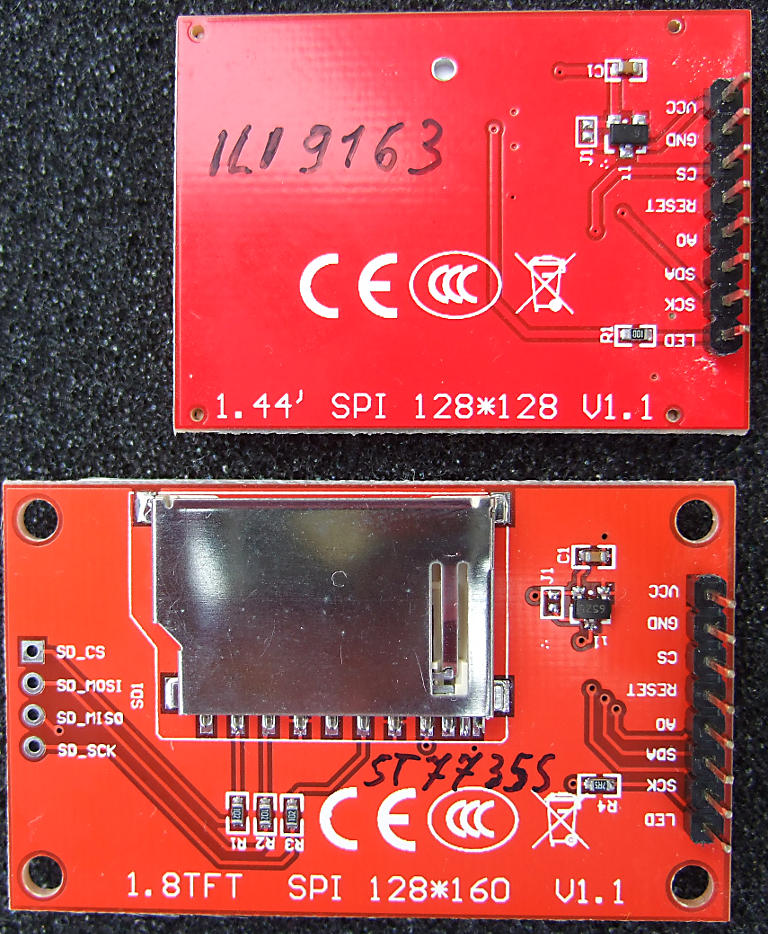
\includegraphics[width=8cm]{../PNG/Color_ILI9163_ST7735.jpg}
\caption{Back side of two Color-LCD's}
\label{fig:Color_both}
\end{figure}

The 128x128 pixel modul uses a ILI9163 controller.
The 128x160 pixel modul uses a very simular ST7735 controller.
The modules are tested with a adapter board, which connects the
SPI signals and the power to the terminal for the normal character display.
The adaption of the \(5V\) output signals of the ATmega to the \(3.3V\) inputs of the controller
is ensured with serial \(10k\Omega\) resistors.
The background light (LED) is required for this modules because nothing is readable without it.
Because of the high count of pixels in vertical direction you can display more text lines for this modules.
For the 128x128 pixel display you can display 8 lines of text with a 12x8 font,
for the 128x160 pixel display you can evel show 10 lines of text.
At the picture \ref{fig:Color_PNP} you can see the result of the measurement of a Germanium transistor
at a 128x128 pixel display.

\begin{figure}[H]
\centering
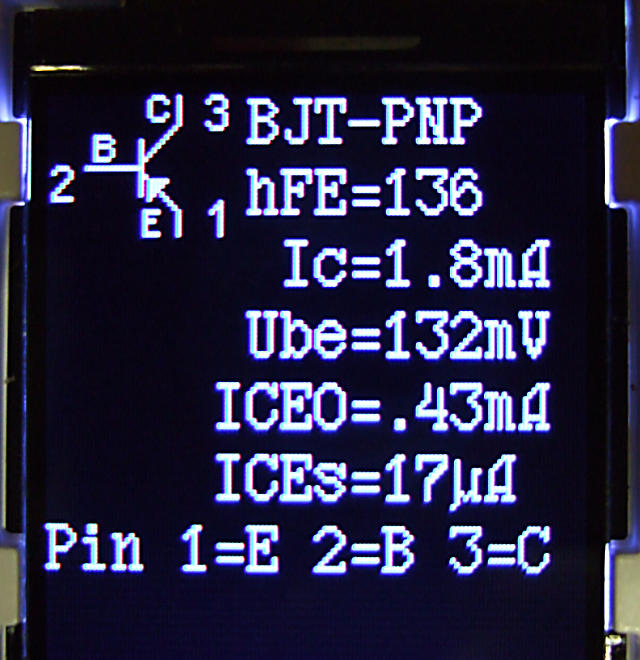
\includegraphics[width=8cm]{../PNG/Color_PNP_ILI9163.jpg}
\caption{Measurement of a bipolar PNP transistors}
\label{fig:Color_PNP}
\end{figure}

The color feature of the modules is currently not used.
Simply the background color and the foreground color can be changed in the file lcd\_defines.h or
in the Makefile.
The 16-bit color model of the controller is used by the software, the foreground color can be changed
with the constant LCD\_FG\_COLOR and the background color with the constant LCD\_BG\_COLOR .


\section{Hints for building the TransistorTester}
Every LCD-display with at least 2x16 character and a HD44780 compatible controller
can be used with the TransistorTester. You should respect the current needed for
illumination, some LCD need lower current than others.
I had tried OLED type displays, but this type cause interference with measurements
of the ATmega and are {\bf not} recommended. Also loading of special characters
for displaying the resistor symbol has caused problems with the OLED.

The resistors R1 to R6 are critical for measurements and this \(680\Omega\) and
\(470k\Omega\) resistors should be measurement type resistors (tolerance of 0.1\%) to
get the full accuracy.
You should use a precision socket for the ATmega microcontroller to enable
the replacement of the microcontroller.
The microcontroller ATmega8, ATmega168 and ATmega328 can be used.
Recommended is a ATmega328, if you wish to use all features.

Anyway you should assemble all parts to printed board without the microcontroller.
A up-to-date low voltage drop regulator like MCP1702-5002 is recommended as IC2, because it
need only \(2\mu A\) of standby current and can still deliver \(5V\), if your input
voltage is only \(5.4V\). But this part is not pin compatible to well known 78L05 with TO92 body!

After checking, that all needed parts are at the correct place, you should
first connect the battery or power supply to the printed board without LCD-display
and microcontroller. You should check the voltage at the power pins of the
microcontroller and LCD-display terminal during the Test key is pressed.
The voltage should disappear, if you release the Test key.
If the voltage had correct polarity and value,
you should disconnect the power and assemble the microcontroller with correct
alignment. Be careful and make sure, that all pins of the microcontroller
are in the socket holes.
Now you can also connect the LCD. Check if power pins of the LCD has the right connection to
GND and VCC of your board.

If you are sure that everything is all right, reconnect the power. 
If you have already programmed the ATmega, you can press the Test button.
By pressing the Test key, the background light of the LCD should switch on.
If you release the Test button, the LED should illuminate weak.
Notice, that the software for the microcontroller must be compiled for the
correct processor type. A program for the ATmega8 does not run on a ATmega168!

\section{Changeover for tester versions designed by Markus F.}
\label{sec:change_markus}
\begin{description}

\item[Voltage control]
If the problem exist, the tester will shut down immediately with every switch on.
With imy suggested setting of the fuses (Makefile) the voltage control of the different
ATmega versions is switched to \(4V\) (brown out level).
This may be the reason why the tester makes trouble with the power on sequence.
The Pin PD6 tries to switch the 100nF capacitor C2 to VCC level causing a voltage
breakdown of the VCC voltage (\(5V\)).
The capacitor C2 can be reduced to \textless~\(10nF\) without problems.
If possible, the direct connection of PD6 should be replaced by a resistor \textgreater~\(220\Omega\).
\item[Improvement of power on circuit]
Often this problem is the reason, if the tester starts with the button hold pressed, but switch off
directly by releasing. The problem is enforced by a high current background light for the LCD.
The resistor R7 to the base of the PNP transistor T3 was optimized with the value \(27k\Omega\) 
too much to save power consuming.
To improve the switching with lower battery voltage or lower current amplification factor of
the PNP transistor T3, you should reduce the resistance to \(3.3k\Omega\).
\item[Additional pull-up resistor at PD7]
The missing pull-up resistor results to a switch off of the tester with the message ''Timeout''
after a short display time.
The software is configured with the option PULLUP\_DISABLE, that all internal pull-up
resistors are switched off. For that reason the voltage of pin PD7 is not definded,
if the level is not switched by the push button or transistor T2 to GND.
One external pull-up resistor of \(27k\Omega\) to VCC avoid this error.
\item[Capacitor C1 at the AREF pin]
Many designs use a \(100nF\) capacitor at the AREF pin, like the design of Markus F. too.
As long as the reference voltage of the ADC is never changed, this is a good solution.
The software of the TransistorTester for the ATmega168/328 uses a automatic selection
of the internal \(1.1V\) reference voltage of the ADC, if the input voltage is below \(1V\).
With this solution a better resolution of the ADC can be reached for little input voltages.
Unfortunately the switching from \(5V\) to \(1.1V\) reference is very slowly. A additional
wait time of \(10ms\) must be respected for this reason.
With changing the capacity value to \(1nF\) this wait time can be reduced significant.
I have not noticed any degration of measurement quality with this change.
Even a removing of the capacitor has no significant change of measurement results.
If you prefer to leve the capacitor unchanged, you can remove the option NO\_AREF\_CAP
in the Makefile to activate longer wait times in the program.
\item[Expanding of a \(8MHz\) crystal]
With some skill you can expand a \(8MHz\) crystal to the backside of the printed board
directly to the pins PB6 and PB7 (pin 9 and pin 10).
My own expansion was done without the both \(22pF\) capacitors.
This solution has operated well with all tested ATmega.
But it is not required to use a crystal. You can still use the \(8MHz\) RC oszillator
by setting the fuses to get the better resolution of time constant for measuring  the capacity values.
\item[Smoothing of the operating voltage]
The original circuit of Markus F. shows only one \(100nF\) capacitor to block the VCC voltage.
This is clearly too little smoothing. You should at least use one \(100nF\) near the ATmega power pins
and one near the voltage regulator. The input of the voltage regulator should be
blocked with a \(100nF\) too.
Additional \(10\mu F\) capacitors (electrolytic or ceramic) at the input and
output of the voltage regulator can stable the voltage level.
Ceramic \(10\mu F\) capacitos with SMD mounting form are easier to use for backfitting
and have usually a lower ESR value. 
\item[Selection of the ATmega processor]
The using of the base function of the tester is still possible with a ATmega8.
The flash memory of that device is used near \(100\%\).
Because the ATmega168 or ATmeg328 processors are pin-compatible to the ATmega8,
I can recommend the replacement.
Actually the price for ATmega328 is so cheap, that there is no reason to take
a ATmega168 type.
With a ATmega168/328 you get the following advantages:
Self test with automatic calibration.\\
Improvement of measurement quality by automatic switching of ADC scale.\\
Measurement of inductors with resistance  below \(2100\Omega\).\\
Measurement of ESR value of capacitors with value of above  \(20nF\).\\
The resolution of resistor measurement below \(10\Omega\) is \(0.01\Omega\).\\
Using of pin PC4 as serial output.\\
\item[Missing precision voltage reference]
Usually the software should detect the missing voltage reference with the unconnected pin PC4.
In this case no VCC=x.xV message should appear in row 2 of the LCD on power on.
If this message appear without the reference, you should connect a \(2.2k\Omega\) resistor
to the PC4 input and VCC.


\end{description}

\section{Chinese clones with text display}
As I know, the tester is rebuild in China in two versions with character displays.
The first model is rebuild from the first design of Markus F. without the ISP port.
The assembled ATmega8 is placed in a socket, so you can replace it with a ATmega168 or ATmega328.
For this version you should consider all the hints of section \ref{sec:change_markus}.
Additional \(100nF\) ceramic cpacitors should be connected near by the VCC-GND and AVCC-GND pins of
the ATmega for better stabilization of the power voltage.
Because there is no ISP connector at the board, you must expand the board with a ISP connector or you
must plug the ATmega to a external socket for programming.
In addition you should notice, that if your ATmega should run with a \(8MHz\) crystal,
your external ISP programmer must have a external clock for programming or a crystal mounted at the socket.\\

The second version of rebuilded tester is build with SMD components. Also the fix installed ATmega168
is a SMD type with 32TQFP body.
Fortunately on the board is a 10-pole ISP connector provided for the programming.
I have analysed the board version ''2.1 2012/11/06''. One error is the assembly of the part ''D1'',
which should be a precision \(2.5V\) voltage reference. Assembled is only a zener diode.
This part should be removed. You can mount a LM4040AIZ2.5 or LT1004CZ-2.5 precision voltage reference
at this place. A missing voltage reference is noticed by the software, so that you must not install
the voltage reference.
My exemplar was delivered with software version 1.02k. The 10-pole ISP plug was not assembled and I must
install a jumper from ISP pin 6 to ISP pin 10. My programmer expect a GND connection at pin 10, but the
board has GND level only on pin 4 and pin 6 of the ISP.
The label of the ATmega168 was rub away and there was no documentation delivered with the part.
The lock fuses of the ATmega were set, so no readout was possible.
But I could install the software version 1.05k without any problems.
Another user has problems with the same software version 1.05k. This user has the chinese board ''2.2 2012/11/26''.
The software runs only without problems, if a additional \(100nF\) keramic capacitor was placed between
the pin 18-AVCC and 21-GND near by the ATmega.
The software 1.05k uses the sleep state of the ATmega for waiting time. For this reason the current alternates
often and the voltage regulator is stressed more.
Further I have noticed, that the VCC voltage is blocked with a \(100nF\) ceramic capacitor and with a
\(220\mu F\) electrolytic capacitor nearby the 78L05 voltage regulator.
The \(9V\) supply voltage is blocked with the same capacitors, but not at the input of the regulator but
at the emitter of the PNP transistor (parallel with the battery). 
The printed circuit board track from the ATmega168 to the test port is very thin, so that a resistance
of \(100m\Omega\) could be measured for one path. This will be the reason for measuring a resistance
of \(0.3\Omega\) for two direct connected pins.
The ESR measuring can usually consider this by zero compensation.
Beginning with version 1.07k  the software does respect this offset for measuring resistors below \(10\Omega\) too.

\section{Chinese clones with graphical display}
Newer rebuilds of the tester like a version from Fish8840  use a 128x64 pixel graphical display.
This version use a modified circuit for the switch on logic. 
The figure \ref{fig:Fish8840} shows a part of the modified circuit.

\begin{figure}[H]
\centering

\includegraphics[width=12cm]{../FIG/Fish8840.eps}
\caption{Part of the circuit from the Fish8840 version}
\label{fig:Fish8840}
\end{figure}

How you can see at the values of resistor R8 and R15,
a 2:1 scaling factor for the battery voltage measurement is used instead of the original scaling factor.
In addition R15 is direct connected to the battery, what results to a power consumption in the switch off state.
The R15 should better be connected to the drain of Q1 or the input of the voltage regulator to prevent this
unneeded battery power consumption.
A suitable change of the printed board is shown in picture \ref{fig:Fish8840patch}.
A circuit path is cut between R17 and D5 and a new conductive path is inserted between Q1 and
R15 with a enameled copper wire.

\begin{figure}[H]
\centering
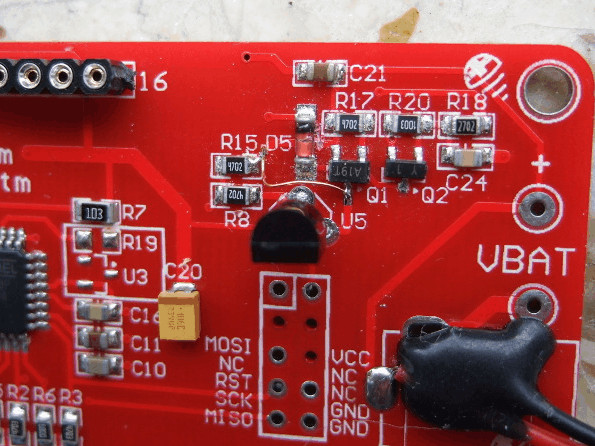
\includegraphics[width=12cm]{../PNG/Fish8840patch.jpg}
\caption{Picture of the changed Fish8840 printed board}
\label{fig:Fish8840patch}
\end{figure}

The scaling factor of the battery voltage must be specified in any case in the Makefile before any
attempt can be done to replace the original software (BAT\_NUMERATOR=66 for example).

The display module of the Fish8840 tester is equipped with a \(3.3V\) voltage regulator to adapt
the operating voltage of the display controller.
Because the \(3.3V\) operating voltage can be increased with the \(5V\) signal level of the data signals
from the ATmega, a adapter circuit according to the picture \ref{fig:Fish8840Adapt} is recommended.
The four data signal lines are equipped with four serial \(2.7k\Omega\) resistors at a little
breadboard.
Longer spacer bolts must be used to mount the display with the adapter board to the printed board
of the Fish8840 tester now.

\begin{figure}[H]
  \begin{subfigure}[b]{9cm}
    \centering
    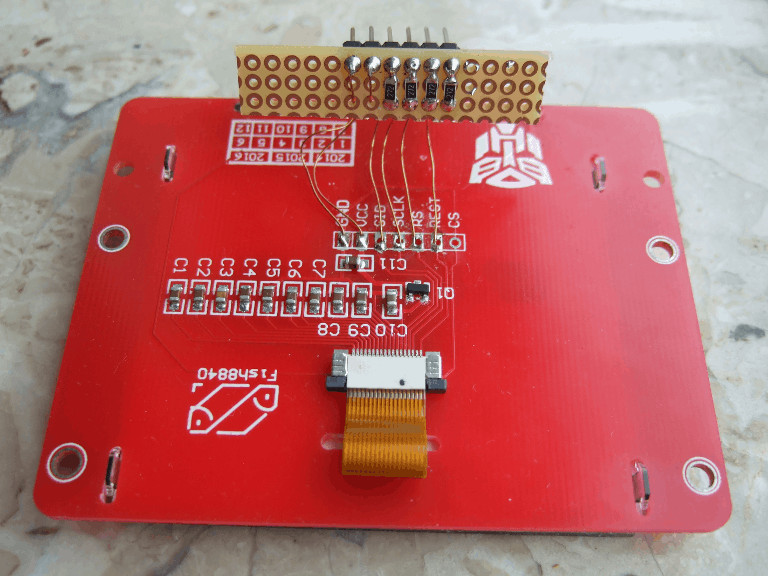
\includegraphics[width=9cm]{../PNG/Fish8840Adapt1.jpg}
    \caption{Display with the breadboard adapter}
  \end{subfigure}
  ~
  \begin{subfigure}[b]{9cm}
    \centering
    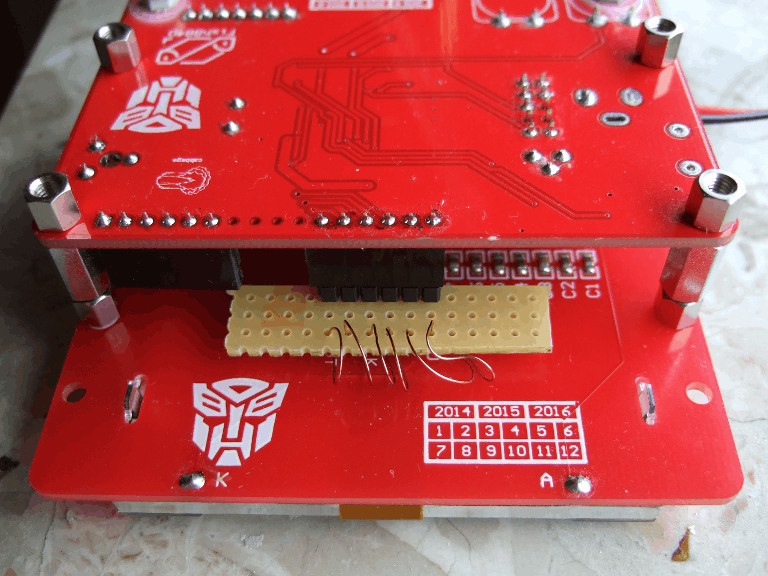
\includegraphics[width=9cm]{../PNG/Fish8840Adapt2.jpg}
    \caption{Ready mounted Tester}
  \end{subfigure}
  \caption{Adapter for a correctly display connection}
  \label{fig:Fish8840Adapt}
\end{figure}

Instead of this modification you can also use a special output mode of the 4~SPI signals of the ATmega
with the Makefile option LCD\_SPI\_OPEN\_COL .
With this option the outputs are not switched to VCC level,
but the internal ''pull-up'' resistors are switched on during the output of a high level.
If the option PULLUP\_DISABLE is set, additionally a external pull-up resistor for
the ''Reset'' signal (PD0) is required.
Because the data signals are never switched to VCC directly, the \(3.3V\) power of the LCD controller
can not be elevated.
My version of the Fish8840 tester has all signals for connecting a character display
routed to the LCD plug connector.
Therefore you can prepare the board for connection of a character display, if the
female header is completed and the potentiometer for the contrast level is added.
However the supply pin 15 for the background light is connected directly to the VCC level.
If you install a character display, you should check, that your display module
is equipped with a serial resistor for the background LED.
Of course iyou have to adapt the software for different displays. 
Also the hardware extension are possible with the Fish8840 board.\\

All attempt to replace the original software is allways done at one's own risk.
No guaranty can be given for operational capability of newer software versions.
Unfortunately the original state of the chinese software can not be saved because the 
security bits of the ATmega328 are set. So there is no way to get back to the original state.\\


A additional version with graphical display is the WEI\_M8 printed board, which is shown in picture~\ref{fig:WeiM8}.
This build use a LiIon accumulator with AA (mignon) size as power supply, which can be loaded
with the micro USB plug. Operating is also possible without the accumulator, only with the USB power.

\begin{figure}[H]
\centering
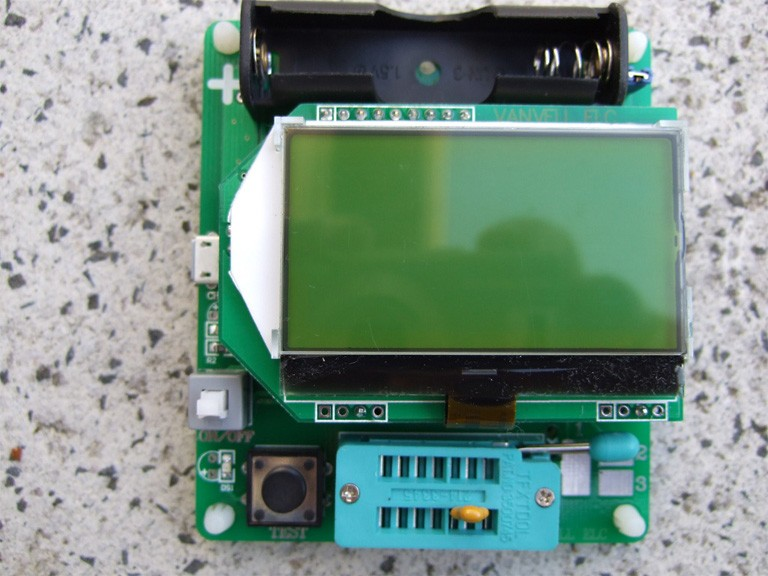
\includegraphics[width=12cm]{../PNG/WEI_M8.JPG}
\caption{Picture of the chinese WEI\_M8 tester}
\label{fig:WeiM8}
\end{figure}

It is pleasant, that the signal lines of the display are equipped with serial resistors
at the adapter board, as you can see in the left picture of~\ref{fig:WeiM8int}.
Therefore you must not be afraid that the \(5V\) signals of the ATmega can cause a excessive
increase of the \(3.3V\) power of the display controller.

\begin{figure}[H]
  \begin{subfigure}[b]{9cm}
    \centering
    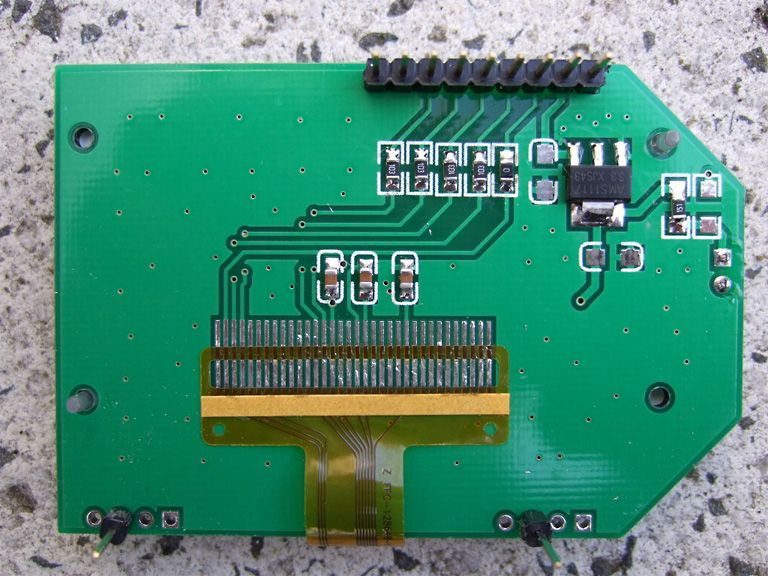
\includegraphics[width=9cm]{../PNG/WEI_M8_D.JPG}
    \caption{Adapter board for the display}
  \end{subfigure}
  ~
  \begin{subfigure}[b]{9cm}
    \centering
    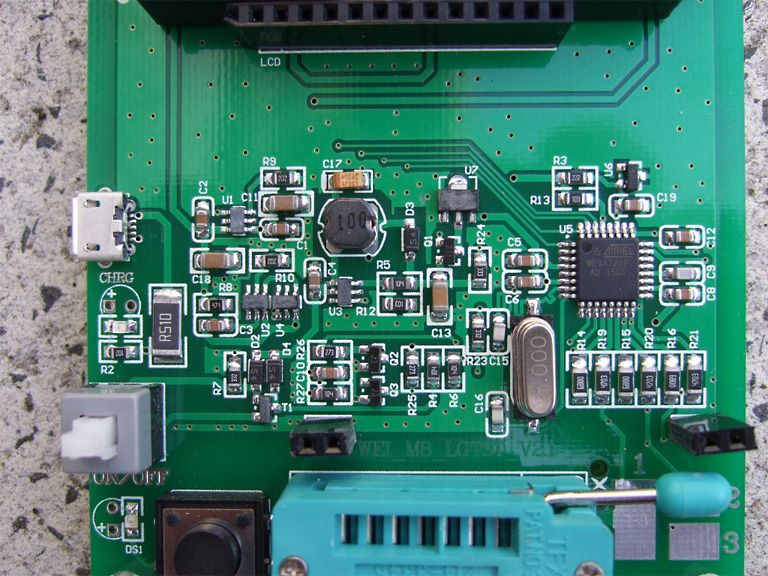
\includegraphics[width=9cm]{../PNG/WEI_M8_L.JPG}
    \caption{Base board}
  \end{subfigure}
  \caption{Inside look to the WEI\_M8 Testers}
  \label{fig:WeiM8int}
\end{figure}

With the upgrade to version 1.12k some problems has occured.
If the extended fuse is set to 0x04 (0xfc) as recommended, some measurements has
caused a ''Brown Out'' reset of the processor.
This resets are caused by short voltage drops of the VCC power.
I have added a additional \(4.7\mu F\) ceramic capacitor at the input side of
the voltage regulator and a \(10\mu F\) ceramic capacitor at the output side (VCC)
of the regulator.
Both before and after the upgrade I have noticed, that with bipolar transistors
a residual collector current (ICEO or ICEs) of about \(1\mu A\) was detected with this board.
Not until the unknown LDO voltage regulator was replaced with a MCP1702-5002 this
effect has disappeared. The figure \ref{fig:WeiM8mod} shows the modified board with
the slantwise mounted capacitors and the MCP1702 regulator.
If you don't wont to modify your board, you must set the extended fuse to 0x07 (0xff)
to enable a regular operation. With that setting the voltage drops remain undetected.

\begin{figure}[H]
\centering
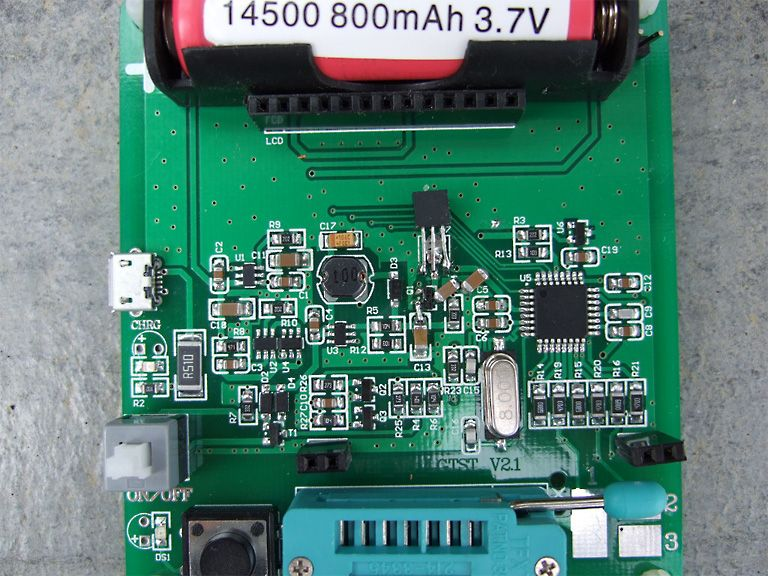
\includegraphics[width=12cm]{../PNG/WEI_M8_modified.JPG}
\caption{Picture of the modified WEI\_M8 Tester}
\label{fig:WeiM8mod}
\end{figure}

A additional chinese version with graphical display is the ''LCD-T4'' tester with a yellow 
printed board.
I have removed the display for replacing the software with a newer version.
At the right picture of figure~\ref{fig:T4_front} you can see in the right upper corner the ISP male connector
with correct orientation beside the six holes of the board.
For programming the ATmega I have not soldered the male connectorr. I have only pugged it into
the holes instead and have fixed it with a finger during the programming.
With that procedure the male connector can be easy removed an the display can be mounted again to
it's origin place.
The chinese software could be replaced with the 1.12k without any noticeable problem. 
Also the activating of the ''brown-out'' monitor by setting the extended fuse has not
shown any surprice.

\begin{figure}[H]
  \begin{subfigure}[b]{9cm}
    \centering
    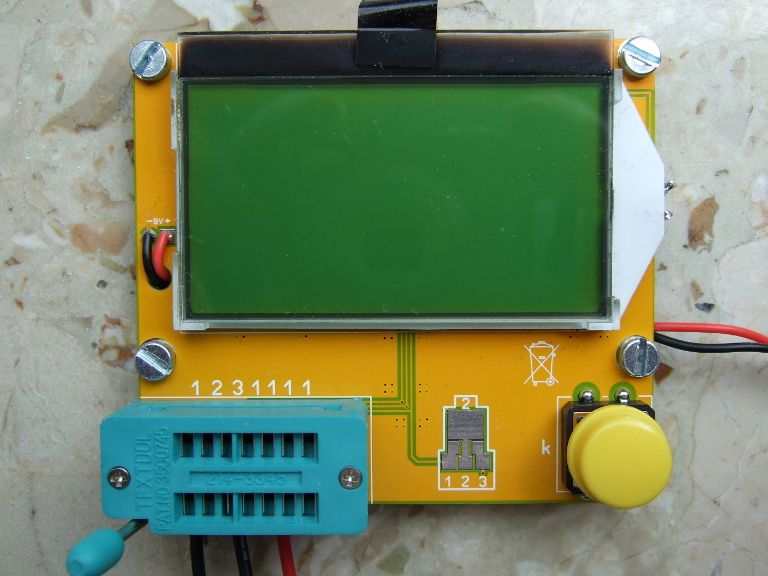
\includegraphics[width=9cm]{../PNG/T4_front.JPG}
    \caption{completely}
  \end{subfigure}
  ~
  \begin{subfigure}[b]{9cm}
    \centering
    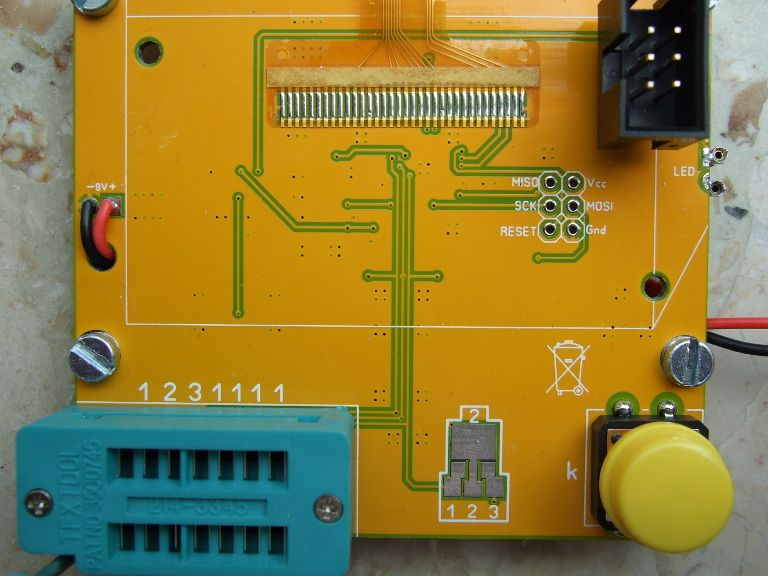
\includegraphics[width=9cm]{../PNG/T4_front_noLCD.JPG}
    \caption{with removed display}
  \end{subfigure}
  \caption{Front view of the T4 tester}
  \label{fig:T4_front}
\end{figure}

You can see the upgraded \(5mm\) threaded bolt and the upgraded cables with measurement clips
at the pictures of the back side in figure \ref{fig:T4_back}.
Because the data signals for the graphical LCD controller have also no
level adaption (\(5V\) -\textgreater~\(3.3V\)), the setting of the option LCD\_SPI\_OPEN\_COL is recommended.
Due to the fact, that the board can not be easy upgraded with a ''pull-up'' resistor,
it make sense to remove the option PULLUP\_DISABLE instead. 
This board is lesser practical for later extensions, a replacement of the display is
also difficult to realize.

\begin{figure}[H]
  \begin{subfigure}[b]{9cm}
    \centering
    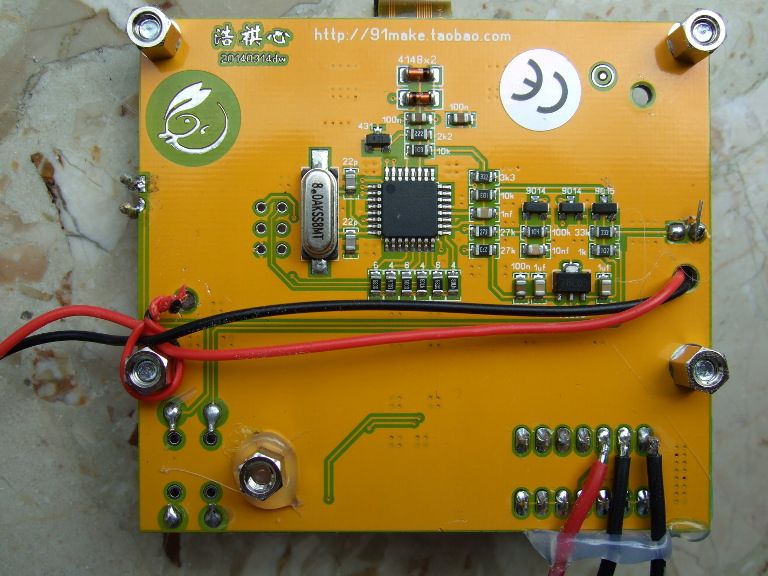
\includegraphics[width=9cm]{../PNG/T4_back.JPG}
    \caption{components side}
  \end{subfigure}
  ~
  \begin{subfigure}[b]{9cm}
    \centering
    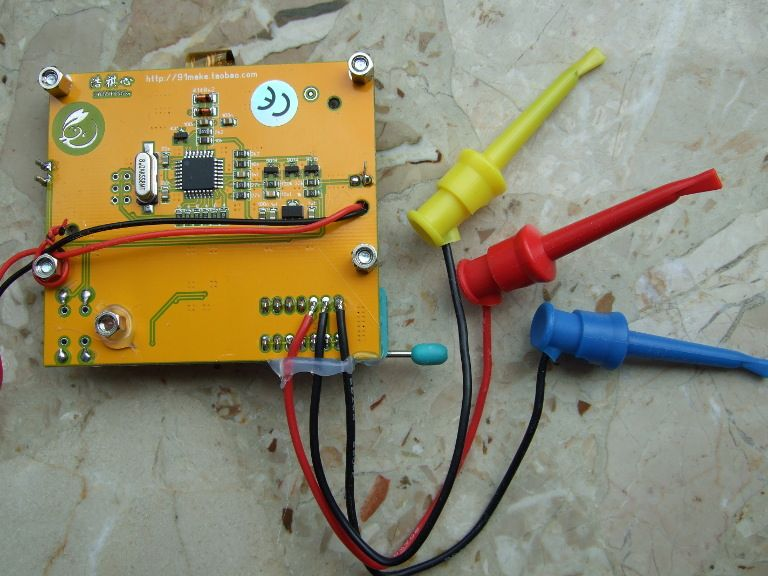
\includegraphics[width=9cm]{../PNG/T4_back_clips.JPG}
    \caption{with measurement cables}
  \end{subfigure}
  \caption{Back side of the T4 tester}
  \label{fig:T4_back}
\end{figure}

A additional chinese version with graphical display is offered with the name ''GM328''.
For this version the graphical display is connected with a adapter circuit board to the 16-pol female connector. 
The port PD5 of the ATmega is connected via pin 6 of the female connector to the CE (Chip Enable) input of the 
graphical controller.
The signal CE is also conneted at the adapter board to the \(0V\) power (GND).
This will resulte to a short-circuit if the ATmega will switch the PD5 output to \(5V\).
But newer versions of the software also switch the CE signal, even if the signal is not necessary for
correct operation.
For correct operation of the ''GM328'' tester with newer software versions you should cut the
connection of the CE signal to pin 6 of the male connector.

\section{Chinese kits with graphic displays}

Two different kit versions with graphical display and rotary encoder are known until now.
The first released kit use a display with a ST7565 or compatible controller (128x64 pixels).
In addition to the rotary encoder a additional input for frequency measurement is provided.
For the test ports a 14-pin Textool socket, three soldering pads for cables and a testpad
for SMD parts are provided at the main board.
The pictures~\ref{fig:Kit_mono} shows the mounted kid.
One of the both \(22 pF\) capacitors was replaced with a trimmer at the soldering side.
With a trimmer the frequency of the crystal can be adjusted for better accuracy of frequency measurement
and frequency generation. 

\begin{figure}[H]
  \begin{subfigure}[b]{9cm}
    \centering
    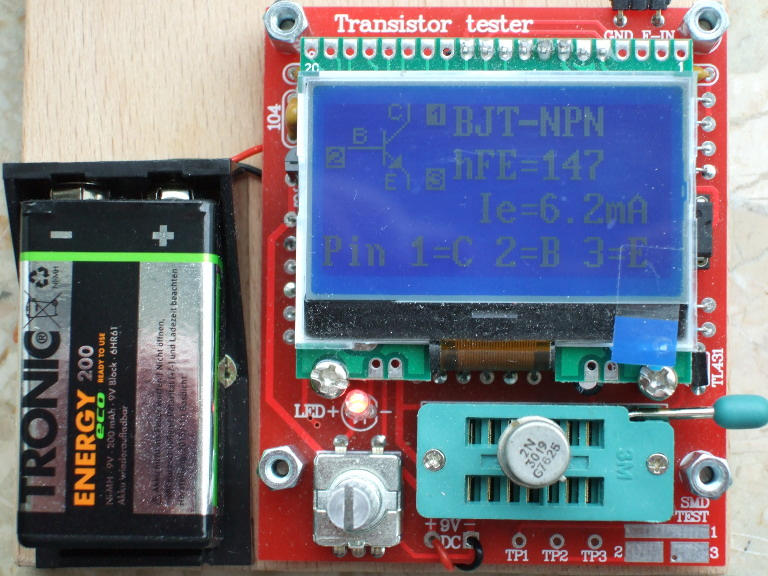
\includegraphics[width=9cm]{../PNG/Kit_ST7565a.jpg}
    \caption{build together}
  \end{subfigure}
  ~
  \begin{subfigure}[b]{9cm}
    \centering
    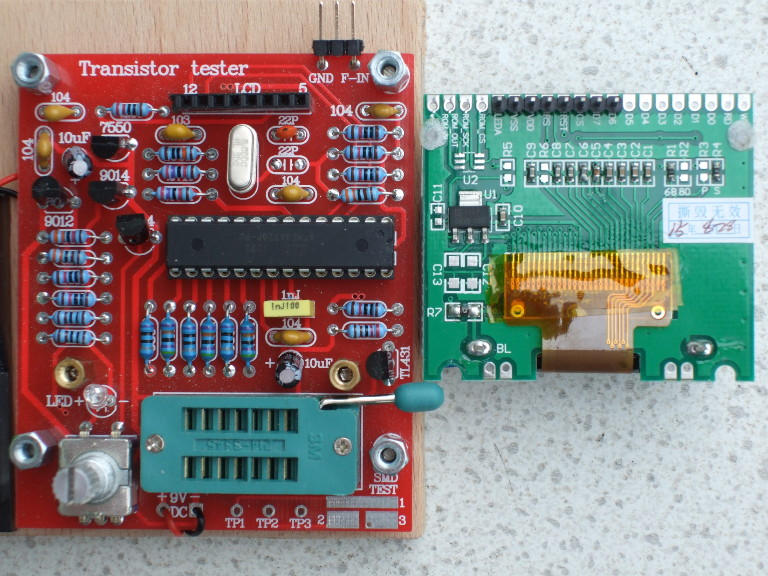
\includegraphics[width=9cm]{../PNG/Kit_ST7565b.jpg}
    \caption{with dismounted display}
  \end{subfigure}
  \caption{Assembled kit with 128x64 pixel display}
  \label{fig:Kit_mono}
\end{figure}

The later released kit use a color display with a ST7735 controller (160x128 pixel)
and is additionally equipped with a input for voltage measurement and a terminal for frequency output.
But the frequency output terminal is not buffered, it is simply connected parallel to the TP2 terminal.
The voltage measurement can handle positiv DC voltages up to 50V. A additional DC-DC converter
for the measurement of Zener diodes is not provided. 
The pictures~\ref{fig:Kit_color} shows this assembled kit.
Also in this version was one of the both \(22 pF\) capacitors replaced
by a trimmer (green color).

\begin{figure}[H]
  \begin{subfigure}[b]{9cm}
    \centering
    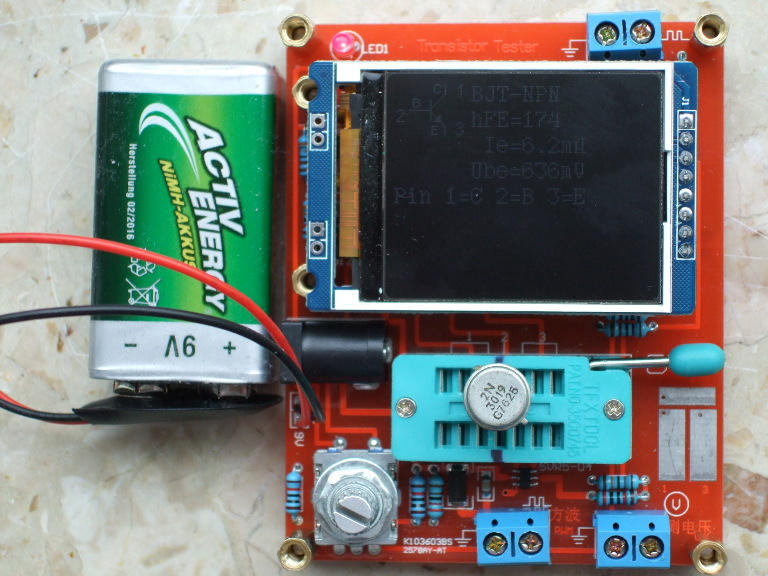
\includegraphics[width=9cm]{../PNG/Kit_Color_a.jpg}
    \caption{build together}
  \end{subfigure}
  ~
  \begin{subfigure}[b]{9cm}
    \centering
    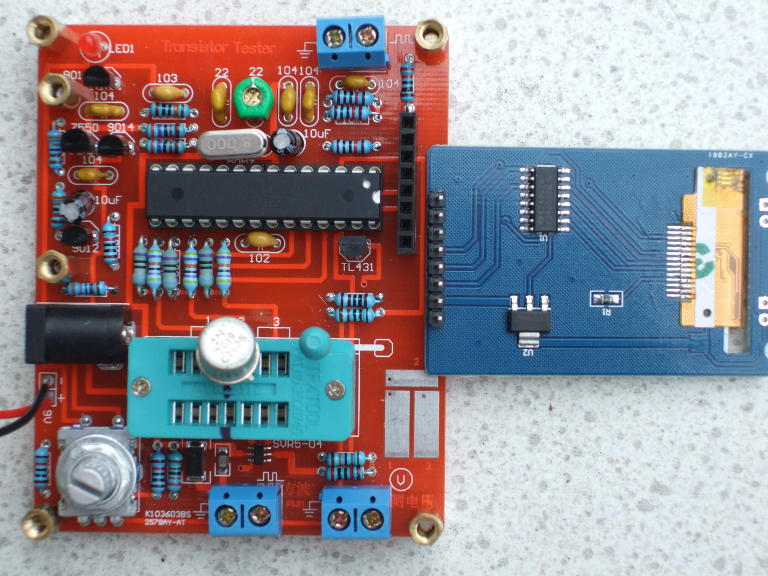
\includegraphics[width=9cm]{../PNG/Kit_Color_b.jpg}
    \caption{with dismounted display}
  \end{subfigure}
  \caption{Assembled kit with 160x128 pixel color display}
  \label{fig:Kit_color}
\end{figure}

Both kids use a DIP version of the ATmega328P mounted at a sockets and are
not equipped with a ISP connector for updating the ATmega with newer software versions.
The first version use
only leaded parts for the main circuit board. 
I have received measurement resistors \(680\Omega\) and \(470k\Omega\) with 0.1\% tolerance
with the Chinese kit. Also a \(220 nF\) capacitor for calibration was added
to the kit.
The kit with the color display was equipped with a connector for a DC power supply additionally
to the pads for the 9V battery.
Some few SMD parts was allready assembled at the main board, so that also only simple soldering
tasks are to do for this kit. 
A little disadvantage of the version with the color display is the speed of display output.
Especially for the menu handling the slower output speed will be noticed.
Otherwise the color display has a significant higher count of pixels, so more text can be shown at once.
Both kits use a 3.3V voltage regulator for the power of the display controller at the
full assembled display circuit boards.
Only the pin header must be soldered at the display circuit board.
The color version use a CD4050 buffer to adapt the different signal voltage levels.
I did not found any adaption of signal voltage levels at the board for the ST7565 version.
Probably the selected controller version tolerates the 5V signal levels of the ATmega328.
I could not find protection diodes at the input signals to the 3.3V supply side for this controller type.


\section{Extented circuit with ATmega644 or ATmega1284}

A extended circuit for ATmega644/1284 processors was developed with Nick L. from the Ukraine.
The circuit \ref{fig:t644tester} enables a additional test of crystals and a extended range
for the frequency measurement.
Although the basic circuit is very simular to the circuit \ref{fig:ttester}, the
port assignment is different.
A rotary pulse encoder with circuit \ref{fig:RotExt} can be connected here at the pins PB5 and PB7 (instead of PD1 and PD3).
Both signals and also the power signals VCC and GND are available at the ISP connector,
so that the extension can also be connected here.\\

The 16:1 frequency divider of the 74HC4060 is allways used for frequencies above \(2MHz\).
The frequency divider can also be used for frequencies between \(25kHz\) and \(400kHz\) to
upgrade the frequency resolution by using the period measurement.
For switching between the operational states (frequency divider and crystal oszillator)
the analog switches 74HC4052 are used.
The table \ref{tab:mega644-display} shows the pin assignments for the ATmega324/644/1284
microcontrollers for different display connections.
The using of the I\textsuperscript{2}C interface is only possible with the SSD1306 controller.
The signals of the I\textsuperscript{2}C interface require a pull-up resistor of \(4.7k\Omega\) to \(3.3V\).
The outputs of the ATmega is only switched to \(0V\) for the I\textsuperscript{2}C signals.


\begin{table}[H]
  \begin{center}
    \begin{tabular}{| c || c | c | c | c |}
    \hline
      Port & Character LCD &  Graphic LCD  & Graphic LCD  & additional function\\
           &               &  SPI 4-wire   &   I\textsuperscript{2}C        &            \\
    \hline
    \hline
    PB2    &  LCD-RS         &            &             &       \\
    \hline
    PB3    &  LCD-E          &  (LCD-CE)  &  LCD-SCL    &       \\
    \hline
    PB4    &  LCD-D4         &  LCD-REST  &  LCD-SDA    &       \\
    \hline
    PB5    &  LCD-D5         &  LCD-RS    &             & ISP-MOSI \\
           &                 &            &             & Rotary encoder 2 \\
    \hline
    PB6    &  LCD-D6         &  LCD-SCLK  &             & ISP-MISO \\
    \hline
    PB7    &  LCD-D7         &  LCD-SI    &             & ISP-SCK  \\
           &                 &            &             & Rotary encoder 1 \\
    \hline
    \end{tabular}
  \end{center}
  \caption{Different variations of the display port assignments}
  \label{tab:mega644-display}
\end{table}

You can also connect a display with the NT7108 (KS0108, S6B0108) controller to the ATmega644 or ATmega1284 by using
a little circuit as shown in figure~\ref{fig:NT7108lcd_644}.
You should also respect the different pin assignments of display modules with NT7108 controllers as 
shown in table~\ref{tab:NT7108types} at page~\pageref{tab:NT7108types}.

\begin{figure}[H]
  \begin{subfigure}[b]{9cm}
    \centering
    
\includegraphics[width=8cm]{../FIG/ST7108serial164_644.eps}
    \caption{with 74HCT164}
  \end{subfigure}
  ~
  \begin{subfigure}[b]{9cm}
    \centering
    
\includegraphics[width=8cm]{../FIG/ST7108serial595_644.eps}
    \caption{with 74HCT595}
  \end{subfigure}
  \caption{Connection of a NT7108 Controller to a ATmega644/1284}
  \label{fig:NT7108lcd_644}
\end{figure}


\begin{figure}[H]
\centering

\includegraphics[width=18cm]{../FIG/t644tester.eps}
\caption{Extended Transistor Tester circuit with ATmega644}
\label{fig:t644tester}
\end{figure}


\section{Buildup of a tester with ATmega1280 or Arduino Mega}
The basic circuit of the tester can also be also build with a Arduino Mega with a ATmega1280
or ATmega2560 microcontroller with a shield.
The required connections are shown in figure~\ref{fig:t1280tester}.
The names for the connections of the display signals of the Arduino are shown with green color.
Components with red color identification are not required for operating.
The ATmega2560 controller has many connectors, but only one connector has the required
functions for both techniques of the frequency measurement.
The connector must be used as clock input for a build in counter and must also be 
used as interrupt source for change of signal level.
This feature is only available for the pin PE6 (T3/INT6).
The other clock inputs of counters PD7 (T0), PD6 (T1), PH7 (T4) and PL2 (T5) can not be 
used as interrupt source for status change.
Unfortunately the PE6 pin is not connected to a pin of the Arduino female connector strip.
The PE5 pin (7) is connected to the connector 3 of the PWM socket strip and
can be jumpered with the PE6 pin (8) of the ATmega2560.
The output signal of the frequency generation is available at the PB6 (OC1B) pin.
This pin is connected to the connector 12 of the PWM socket strip.
The ISP-connector is not required, because the program can be loaded with the bootloader
and the USB interface to the ATmega. With the bootloader there is always a
little delay for the power up start of the program.

\begin{figure}[H]
\centering

\includegraphics[width=18cm]{../FIG/t1280tester.eps}
\caption{TransistorTester circuit with ATmega1280, ATmega2560 or Arduino Mega}
\label{fig:t1280tester}
\end{figure}

Of course you can connect all supported displays also to the ATmega1280 or ATmega2560
as shown in table~\ref{tab:display-1280} .

\begin{table}[H]
  \begin{center}
    \begin{tabular}{| c || c | c | c | c | c | c |}
    \hline
           & Character     &  ST7565     & ST7920       & NT7108       & SSD1306     & additional function \\
      Port & LCD           &    SPI      & seriell      & seriell      &    I\textsuperscript{2}C      & \\
    \hline
    \hline
    PA0    &  LCD-D4       &   LCD-REST  &  LCD-RESET   & HC595-RCK      &             & \\
    \hline
    PA1    &  LCD-D5       &   LCD-RS    &              & LCD-CS2        &             & rotary encoder 2 \\
    \hline
    PA2    &  LCD-D6       &   LCD-SCLK  &              & HC164-CLK      &             & \\
    \hline
    PA3    &  LCD-D7       &   LCD-SI    &              & LCD-CS1        &             & rotary encoder 1 \\
    \hline
    PA4    &  LCD-RS       &             &   LCD-B0     & LCD-RS         &   LCD-SDA   & \\
           &               &             &              & HC164-SER      &             & \\
    \hline
    PA5    &  LCD-E        &   (LCD-CE)  &   LCD-EN     & LCD-EN         &   LCD--SCL  & \\
    \hline
    PA7    &  key signal   &             &              &                &             & \\
    \hline
    \end{tabular}
  \end{center}
  \caption{Connections for different display to the ATmega1280/2560 processors}
  \label{tab:display-1280}
\end{table}


\section{Programming of the microcontroller}
I release the software for the microcontroller with source code.
The developement is done with Linux operationg system (Ubuntu) and
is controlled with a Makefile. The Makefile makes sure, that your
software will be compiled with the prior selected Makefile options. Some constellations
are precompiled with the source. Please take a look to the ReadMe.txt file
in the directory Software/default and to the chapter~\ref{sec:config} at page~\pageref{sec:config}.
The result of compilation have the extensions .hex and .eep .
Usually the names will be TransistorTester.hex and TransistorTester.eep .
The .hex file contains the data for the program memory (flash) of the ATmega processor.
The .eep file contains the data for the EEprom memory of the ATmega. Both data files
must be loaded to the correct memory.

Additionally the operating state of the
ATmega processor must be programmed with the ``fuses''.
If you can use my Makefile and additionally the program avrdude \cite{avrdude}, you need no exact
knowledge of the details about the fuses. You have only to type ``make fuses'' if you
have no crystal or ``make fuses-crystal'' if you have installed the \(8MHz\) crystal to your printed board.
With the ATmega168 series of the microcontroller you can also use ``make fuses-crystal-lp'' to use
a crytal with the low power mode.
Never choose the crystal mode of clock generation, if you don't have installed
the \(8MHz\) crystal. If you are not sure with the fuses, leave them as default
set by manufactor and first bring the the tester to operation in this mode.
Maybe your program runs too slow, if you use program data compiled for
\(8MHz\) operation, but you can correct this later! But a wrong set of fuses may inhibit
later ISP-programming.

\subsection{Using the Makefile with Linux}
You can install packages with Debian based Linux versions by using a package manager as synaptic or dpkg.
The package ``subversion'' must be installed for downloading the sources or the documentation from the SVN archive.
With the command \\
``svn checkout svn://www.mikrocontroller.net/transistortester'' \\
you can download the complete archive.
Of course you can also download only subdirectories of the archive.
For using the Makefile in one of the subdirectories you must install the packages
make, binutils-avr, avrdude, avr-libc and gcc-avr.
Once you must prepare the access to the interfaces for the user.
If you open a consol window and you have also connected a ISP programmer with USB interface,
you can see the recognized USB devices with the command ''lsusb''.
A sample of the result of lsusb you can see here:
\begin{verbatim}
Bus 001 Device 001: ID 1d6b:0002 Linux Foundation 2.0 root hub
Bus 002 Device 003: ID 046d:c050 Logitech, Inc. RX 250 Optical Mouse
Bus 002 Device 058: ID 03eb:2104 Atmel Corp. AVR ISP mkII
Bus 002 Device 059: ID 2341:0042 Arduino SA Mega 2560 R3 (CDC ACM)
Bus 002 Device 001: ID 1d6b:0001 Linux Foundation 1.1 root hub
\end{verbatim}
A Device 58 is detected here a a AVR ISP mkII type (DIAMEX ALL-AVR).
The ID 03eb is a vendor ID and the ID 2104 is a product ID.
Both ID's are required for a entry in the file /etc/udev/rules.d/90-atmel.rules .
In this example the file 90-atmel.rules has one line:
\begin{verbatim}
SUBSYSTEM=="usb", ATTRS{idVendor}=="03eb", ATTRS{idProduct}=="2104", MODE="0660",
GROUP="plugdev"
\end{verbatim}
This entry allow the access to the USB device 58 for members of the group ''plugdev''.
The also detected USB device 59 allows a access to the serial device ''/dev/ttyACM0'' for
members of the group ''dialout''.

Therefore your user identification should be a member of the group plugdev and also
a member of the group dialout.
With the command ''usermod -a -G dialout,plugdev \$USER'' the membership of both groups should be established.
Now the program avrdude should have permission to access both devices.
In a console window you must first change the directory with the command ``cd'' to a proper
subdirectory of the directory trunk.
Now you can change options of the Makefile with any text editor.
For compiling the source you must only type the simple command ``make''.
If the ISP programmer is configured proper in the Makefile, a command ``make upload''
should result to load the program with the ISP interface to the ATmega.
The ``fuses'' of the ATmega must also be set correctly once.
You can achieve this with the command ``make fuses'' or ``make fuses-crystal''.
The program avrdude probably reports a error for setting the extended fuse efuse.
The reading of unused fuse bits is specified as ''1'' for the ATmega, but the
avrdude program mask the unused bits, so that it expect a ''0'' for all unused bits.
Normally the efuse should be set to 0xfc, but avrdude read back 0x04 with the mask.
You can change the file avrdude.conf to change the behaviour of avrdude or
you can set the efuse to 0x04. 
The value for all efuses can be set with the identifier EFUSE\_VAL at the begin of file setup.mk
in the trunk directory.
Probably the fuses are also set correctly with the error message.

\subsection{Using the WinAVR package with Windows}
If you use the Windows operating system, the easiest way to get a correct programmed
ATmega is to use the WinAVR package \cite{winavr1},\cite{winavr2}.
With my patch \cite{winavr3} you can also set the fuses by using the Makefile.
Of course the avrdude program must support your programmer and the configuration
in the Makefile must match to your environment.

The figures \ref{fig:WinAVR1} show the File menu of the graphical user interface of WinAVR for
open the file Makefile and for saving the changed Makefile (Save).

\begin{figure}[H]
  \begin{subfigure}[b]{9cm}
    \centering
    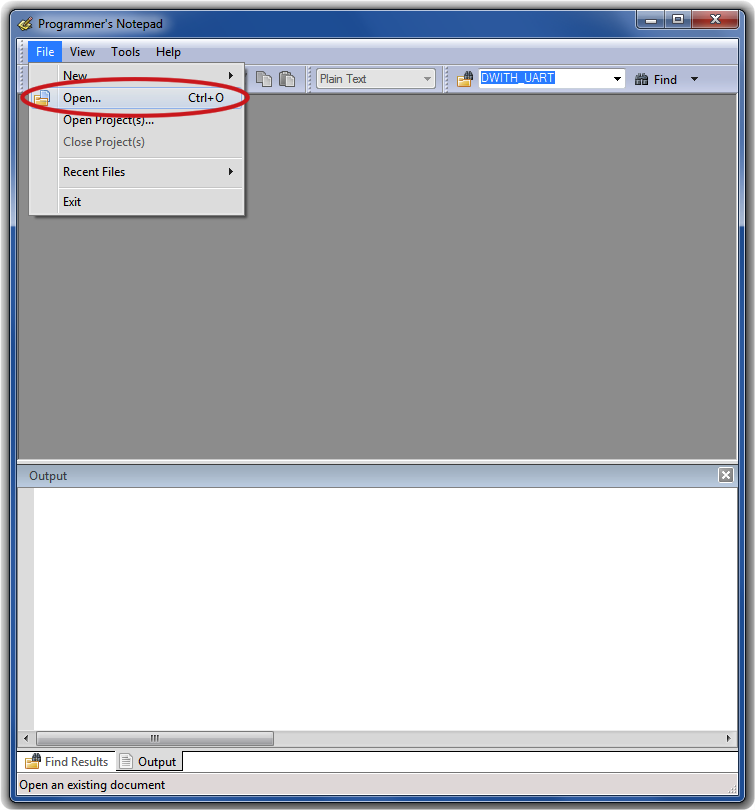
\includegraphics[width=9cm]{../PNG/Notepad_open.png}
    \caption{open Makefile}
  \end{subfigure}
  ~
  \begin{subfigure}[b]{9cm}
    \centering
    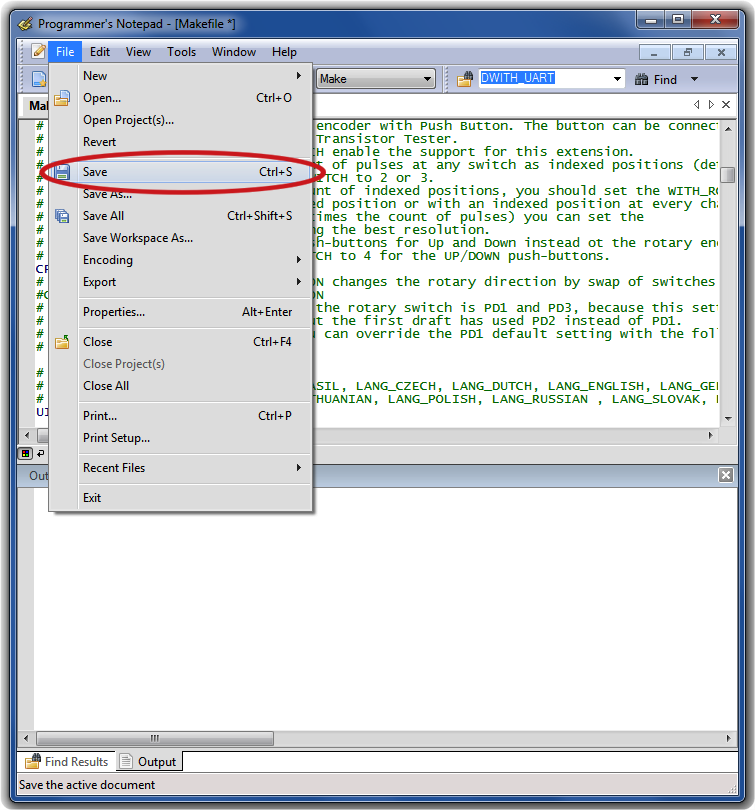
\includegraphics[width=9cm]{../PNG/Notepad_save.png}
    \caption{save Makefile}
  \end{subfigure}
  \caption{Using of the WinAVR user interface Programmer's Notepad}
  \label{fig:WinAVR1}
\end{figure}

The next figures \ref{fig:WinAVR2} show the Tools menu of the Programmer's Notepad
for compiling the program (Make All) and for programming the ATmega (Program) with avrdude.

\begin{figure}[H]
  \begin{subfigure}[b]{9cm}
    \centering
    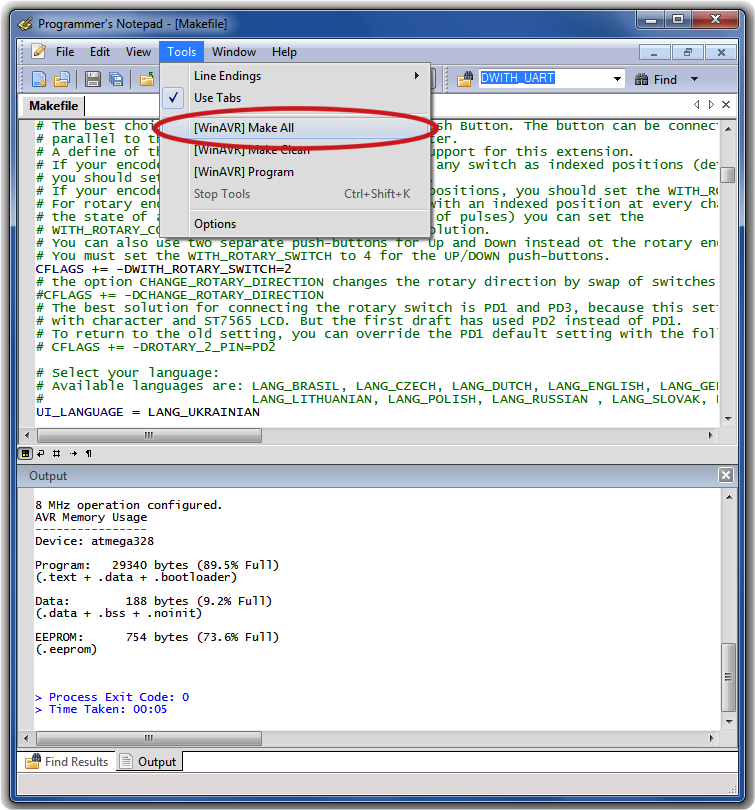
\includegraphics[width=9cm]{../PNG/Notepad_make.png}
    \caption{Build programming data (.hex/.eep)}
  \end{subfigure}
  ~
  \begin{subfigure}[b]{9cm}
    \centering
    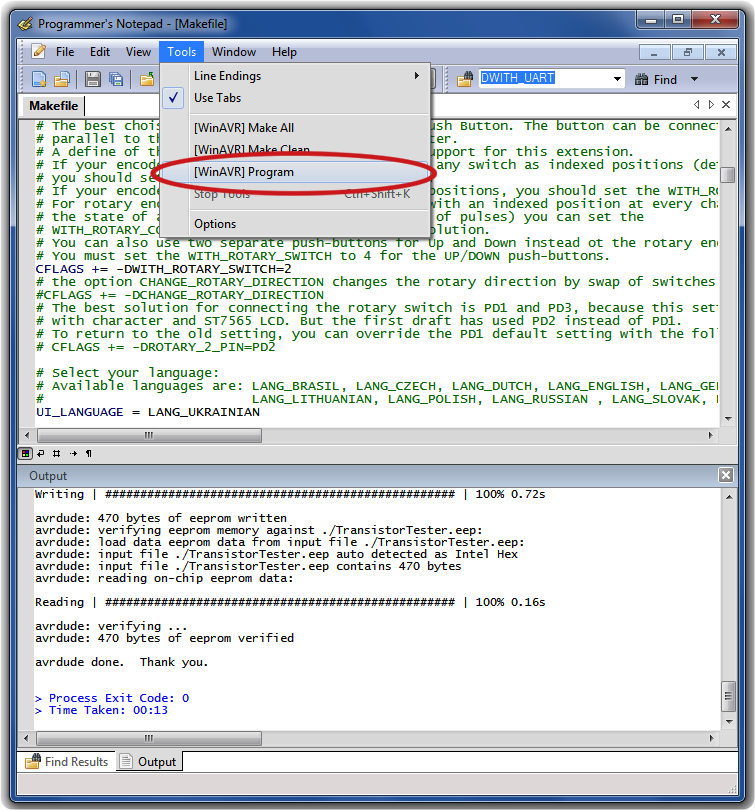
\includegraphics[width=9cm]{../PNG/Notepad_program.png}
    \caption{Programming the ATmega}
  \end{subfigure}
  \caption{Using of the WinAVR user interface Programmer's Notepad}
  \label{fig:WinAVR2}
\end{figure}



\section{Troubleshooting}
In most cases of problems you will miss the text output to the LCD-display.
At first you should check, if the LED was illuminated weak, if you release
the Test button. 
\begin{description}

\item[Power does not switch on.]
If the LED is without light and the VCC power has correct
\(5V\) voltage during holding the Test button, the microcontroller does not switch the power
correctly. The microcontroller should hold the power by switching the
PD6 output to \(5V\), which is usually done as one of the first actions.
If you hold the Test key pressed, the power is switched on anyway.
So you can check the value of VCC power and additionally the voltage value
of the PD6 output, if you hold the key pressed.
If VCC voltage has correct value (\(5V\)), but PD6 voltage is
below \(4V\), your microcontroller does not start the program. In this case
you should check if the microcontroller flash has been loaded with proper data for your
installed type and if ATmega is correctly configured with the fuses.
If your ATmega put the PD6 output to \(5V\) and the power does not stay if you
release the Test key, it is more difficult to find the reason.
First you can shorten the LED and try again. If your Tester now starts,
your LED may be faulty or mounted with wrong polarity. If this is not
the reason, the current amplification factor of your T3 transistor (BC557C)
is insufficient. The current to the base of T3 is lower in the microcontroller
state as in the ``key pressed'' state.

\item[Nothing is readable on the LCD display]
Check the voltage at the contrast pin at the LCD display (pin 3). Adjust to
correct value specified in the data sheet of your display and optimize by viewing.
If you have a high temperature display type, you must provide a negative contrast voltage
for operation. In this case you can use the ICL~7660 device for generating
a negative voltage from positive \(5V\).

The tester software can be configured for many different controller with different connection
types. You should check, if your software matches to your mounted display type.
If there is no output readable on the LCD and the background light is on,
you should disconnect the power and check all four data plus the two control signal connections.
If all connection are well, the only reason I see is a uncorrect timing of
control signals. This can be caused by a slower LCD controller than expected by
the software or the ATmega software runs at wrong clock speed. Please check for which
clock speed your programming data was compiled  and if the fuses of the
ATmega are correct set to that speed. You find the clock parameter in the corresponding
Makefile.
If the tester is build without the switch off electronic, you can test with
a LED connected to the test pins, if the program operates normally.
If the LED flickers, the program operates well. The missing text on the
LCD must be caused by wrong connection or timing.
For some graphical displays the contrast is changeable with a menu function.
If you have changed the contrast value, that nothing is readable at the screen,
you cannot handle the menu function any more. You can try to read the display
from a slanting look to the display, not from the front side.
In this case you can try to handle the menu function with this view.
Otherwise you can write the EEprom data new with a ISP programmer to reset the contrast value.


\item[Something but not all is readable on the LCD display]
Check if the .eep data are loaded to the EEprom memory of ATmega.
If all data are loaded correctly, you should check the clock speed of your
programming data (Makefile) and ATmega processor settings (fuses).

\item[Measurement is slow and Capacitors are measured about 8 times too small]
You run software compiled for \(8MHz\) clock at real clock speed of \(1MHz\).
Please set the fuses of the ATmega correctly.

\item[Measurement has strangely values]
Check if your programmer is still connected to the ISP-plug.
The ISP interface should be disconnected for measuring.
Very often the reason of wrong measurements is the use of software compiled with
the AUTOSCALE\_ADC option and with the option NO\_REF\_CAP, but the capacitor
at the AREF pin has still a value of \(100nF\).
Wrong assembly of components or remaining soft solder flux can disturb the 
measurements too. Please check with the selftest function of your TransistorTester software
if possible. For the details see Chapter \ref{sec:selftest}.

Otherwise inspect your board visually and check the resistor values
with a ohmmeter. You can use the pins of the ATmega for this check, for example
to check the R1 you can measure between pin 23 and pin 14. Take a look at the
circuit diagram \ref{fig:ttester} for details. There is no need to
remove the microcontroller, only battery or power supply should be removed before.

\item[The Tester switch off the power after 2 seconds display time] 
This condition exists, if the external Pull-Up resistor at the PD7 input
is missing or the key button is keep pressed.
The software switch off the internal Pull-Up resistors to prevent a influence
to the measurement results. Therefore a external Pull-Up resistor (27k) is required.

\item[Der Tester shows only Vext=xx.xV in row 2]
This problem exists, if the Pull-Up resistor at the PD7 input
is missing or the key button is keep pressed.
Additionally the software is configured without the serial output (without option WITH\_UART) and
without the internal Pull-Up resistors (with option PULLUP\_DISABLE).
You should install the Pull-Up resistor at pin PD7.


\end{description}


\chapter{Bedienungshinweise}
\label{sec:manual}
\section{Der Messbetrieb}
Die Bedienung des Transistortesters ist einfach.
Trotzdem sind einige Hinweise erforderlich.
Meistens sind an die drei Testports über Stecker-Leitungen mit Krokodilklemmen oder anderen Klemmen angeschlossen.
Es können auch Fassungen für Transistoren angeschlossen sein.
In jedem Fall können Sie Bauteile mit drei Anschlüssen mit den drei Testports in beliebiger Reihenfolge verbinden.
Bei zweipoligen Bauteilen können Sie die beiden Anschlüsse mit beliebigen Testports verbinden.
Normalerweise spielt die Polarität keine Rolle, auch Elektrolytkondensatoren können beliebig angeschlossen werden.
Die Messung der Kapazität wird aber so durchgeführt, dass der Minuspol am Testport mit der kleineren Nummer liegt.
Da die Messspannung aber zwischen \(0,3V\) und maximal \(1,3V\) liegt, spielt auch hier die Polarität keine wichtige Rolle.
Wenn das Bauteil angeschlossen ist, sollte es während der Messung nicht berührt werden. Legen Sie es auf einen
isolierenden Untergrund ab, wenn es nicht in einem Sockel steckt. Berühren Sie auch nicht die Isolation der Messkabel,
das Messergebnis kann beeinflusst werden.
Dann sollte der Starttaster gedrückt werden.
Nach einer Startmeldung erscheint nach circa zwei Sekunden das Messergebnis. Bei einer Kondensatormessung kann es
abhängig von der Kapazität auch deutlich länger dauern.

Was dann weiter geschieht, hängt von der Softwarekonfiguration des Testers ab.
\begin{description}
  \item[Einzelmessung] Wenn der Tester für Einzelmessung konfiguriert ist (POWER\_OFF-Option),
 schaltet der Tester nach einer Anzeigezeit
von 28 Sekunden (konfigurierbar) wieder automatisch aus, um die Batterie zu schonen.
Während der Anzeigezeit kann aber auch vorzeitig eine neue Messung gestartet werden.
Nach der Abschaltung kann natürlich auch wieder eine
neue Messung gestartet werden, entweder mit dem gleichen Bauteil oder mit einem anderen Bauteil.
Wenn die Elektronik zum Abschalten fehlt, wird das letzte Messergebnis weiter angezeigt.

  \item[Dauermessung] Einen Sonderfall stellt die Konfiguration ohne die automatische Abschaltfunktion dar.
Hierfür wird die POWER\_OFF-Option in der Makefile nicht gesetzt.
Diese Konfiguration wird normalerweise nur ohne die Transistoren für die Abschaltung benutzt.
Es wird stattdessen ein externer Ein-/Aus-Schalter benötigt. Hierbei wiederholt der Tester die
Messungen solange, bis ausgeschaltet wird.

  \item[Serienmessung] In diesem Konfigurationsfall wird der Tester nicht nach einer Messung sondern erst nach einer konfigurierbaren
Zahl von Messungen abgeschaltet. Hierfür wird der POWER\_OFF-Option in der Makefile eine Wiederholzahl (z.B. 5) zugewiesen.
Im Standardfall wird der Tester nach fünf Messungen ohne erkanntes Bauteil abgeschaltet.
Wird ein angeschlossenes Bauteil erkannt, wird erst bei der doppelten Anzahl, also zehn Messungen abgeschaltet.
Eine einzige Messung mit nicht erkanntem Bauteil setzt die Zählung für erkannte Bauteile auf Null zurück.
Ebenso setzt eine einzige Messung mit erkannten Bauteil die Zählung für die nicht erkannten Bauteile auf Null zurück.
Dies hat zur Folge, dass auch ohne Betätigung des Starttasters immer weiter gemessen werden kann,
 wenn Bauteile regelmässig gewechselt werden.
Ein Bauteilwechsel führt in der Regel durch die zwischenzeitlich leeren Klemmen zu einer Messung ohne erkanntes Bauteil.

Eine Besonderheit gibt es in diesem Betriebsmodus für die Anzeigezeit. Wenn beim Einschalten der Starttaster nur kurz
gedrückt wurde, beträgt die Anzeigezeit der Messergebnisse nur 5 Sekunden. Wenn der Starttaster bis zum Erscheinen der
ersten Meldung festgehalten wurde, beträgt die Anzeigezeit wie bei der Einzelmessung 28 Sekunden.
Ein vorzeitiger neuer Messbeginn ist aber während der Anzeigezeit durch erneutes Drücken des Starttasters möglich.

\end{description}

\section{Optionale Menüfunktionen für den ATmega328}
Wenn die Menüfunktion eingeschaltet ist, startet der Tester nach einem längeren Tastendruck (\textgreater~\(0.5s\)) ein Auswahlmenü
für zusätzliche Funktionen.
Diese Funktion ist auch für andere Prozessoren mit mindestens 32K Flash Speicher verfügbar.
Die wählbaren Funktionen erscheinen in Zeile~2 eines zweizeiligen Displays oder werden als gekennzeichnete
Funktion in Zeile 3 eines vierzeiligen Displays gezeigt. Dabei wird die vorige und nächste Funktion in Zeile 2 und 4 angezeigt.
Nach einer längeren Wartezeit ohne jegliche Bedienung kehrt das Programm zu der normalen Transistortester-Funktion zurück.
Durch kurzen Tastendruck kann zur nächsten Auswahl gewechselt werden.
Mit einem längeren Tastendruck startet die angezeigte Zusatzfunktion.
Nach Anzeige der letzten Funktion ,,Schalte aus'' wird wieder die erste Funktion angezeigt.\\

Wenn der Tester mit einem Drehimpulsgeber ausgerüstet ist, kann die Menü-Auswahl auch mit einem schnellen
Drehen des Encoders während der Anzeige einer vorausgegangenen Messung aufgerufen werden.
Die Menüfunktionen können mit einem langsamen Drehen des Encoders in beliebiger Richtung ausgewählt werden.
Die ausgewählte Menüfunktion kann aber nur mit einem längeren Tastendruck gestartet werden.
Innerhalb einer Menüfunktion können Parameter durch eine langsame Drehung des Encoders ausgewählt werden.
Eine schnelle Drehung des Encoders kehrt zur Menü-Auswahl zurück.

\begin{description}
 \item[Frequenz]
Die Zusatzfunktion ,,Frequenz'' (Frequenzmessung) benutzt als Eingang den PD4-Pin des ATmega, der auch an das LCD angeschlossen ist.
Es wird immer zunächst die Frequenz gemessen, bei Frequenzen unter \(25kHz\) wird auch die mittlere Periode des Eingangssignals
bestimmt und daraus die Frequenz mit einer Auflösung von bis zu \(0,001Hz\) berechnet.
Bei gesetzter POWER\_OFF-Option in der Makefile wird die Dauer der Frequenzmessung auf 8~Minuten beschränkt.
Die Frequenzmessung wird durch Tastendruck beendet und in das Auswahlmenü zurückgekehrt.\\

 \item[f-Generator]
Bei der Zusatzfunktion ,,f-Generator'' (Frequenz-Generator) können die Frequenzen zwischen 1Hz und 2MHz gewählt werden.
Die Einstellung der Frequenz kann jeweils nur für die höchste dargestellte Stelle (Ziffernposition) verändert werden.
Für die Stellen 1Hz bis 10kHz sind jeweils die Ziffern 0-9 wählbar. Bei der 100kHz Stelle ist 0-20 wählbar.
In Spalte 1 der Frequenzzeile wird durch ein \textgreater~oder \textless~Symbol angezeigt, ob durch einen längeren
Tastendruck (\textgreater~0.8s) zur höheren oder niedrigen Stelle geschaltet wird.
Zur niedrigeren Stelle (\textless) kann nur geschaltet werden, wenn die augenblickliche Stellee auf 0 gestellt wurde
und wenn nicht die Stelle mit 1Hz Schritten gewählt wurde.
Bei der gewählten 100kHz Stelle ist das \textgreater~Symbol durch ein R Zeichen ersetzt. Der längere Tastendruck bewirkt dann eine
Rücksetzung der Frequenz auf den Startwert 1Hz.
Bei gesetzter POWER\_OFF-Option in der Makefile muss für den Frequenzwechsel die Taste länger gedrückt werden, da
durch einen kurzen Tastendruck (\textless~0,2s) nur die Zeitüberwachung von 4~Minuten zurückgesetzt wird.
Die abgelaufene Zeit wird in Zeile 1 durch einen Punkt für jede abgelaufene 30 Sekunden angezeigt.
Durch einen regelmäßigen kurzen Tastendruck kann die vorzeitige Abschaltung der Frequenzerzeugung verhindert werden.
Ein längerer Tastendruck (\textgreater~2s) kehrt wieder zur Auswahl der Funktionen zurück.\\

 \item[10-bit PWM]
Bei der Zusatzfunktion ,,10-bit PWM'' (Pulsweitenmodulation) wird eine feste Frequenz mit einstellbarer Pulsweite an Pin TP2 erzeugt.
Mit einem kurzen Tastendruck (\textless~0,5s) wird die Pulsweite um \(1\%\) erhöht, mit einem längeren Tastendruck um \(10\%\).
Bei Überschreiten von \(99\%\) werden \(100\%\) vom erhöhten Wert abgezogen.
Bei gesetzter POWER\_OFF-Option in der Makefile wird die Frequenzerzeugung nach 8 Minuten ohne Bedienung beendet.
Durch sehr langen Tastendruck (\textgreater~1,3s) kann die Frequenzerzeugung auch beendet werden.\\

 \item[C+ESR@TP1:3]
Bei der Zusatzfunktion ,,C+ESR@TP1:3'' wird eine separate Kondensatormessung mit ESR-Messung an TP1 und TP3 gestartet.
Messbar sind Kondensatoren mit mehr als \(2\mu F\) bis zu \(50mF\). Wegen der geringen Messspannung von etwa 300mV sollte
in vielen Fällen die Messung in der Schaltung ohne vorherigen Ausbau möglich sein.
Bei gesetzter POWER\_OFF-Option in der Makefile ist die Anzahl der Messungen auf 250 beschränkt,
kann aber sofort wieder gestartet werden.
Die Mess-Serie kann durch einen längeren Tastendruck beendet werden.\\

 \item[Widerstandsmeßgerät]
Mit dem \mbox{1 \electricR 3} Symbol wird der Tester in ein Ohmmeter an TP1 und TP3 verwandelt. Diese Betriebsart wird durch
ein {\bf[R]} in der rechten Ecke der ersten Displayzeile angezeigt. Weil bei dieser Betriebsart die
ESR-Meßfunktion nicht benutzt wird, beträgt auch für Widerstände unter \(10\Omega\) die Auflösung
nur \(0.1\Omega\). Wenn die Ohmmeter Funktion mit der Induktitivitätsmessung konfiguriert wurde,
erscheint hier ein \mbox{1 \electricR \electricL 3} Symbol.
Dann beinhaltet die Ohmmeter Funktion die Messung von Induktivitäten für Widerstände unter \(2100\Omega\). 
In der rechten Ecke der ersten Zeile des Displays wird dann ein {\bf[RL]} angezeigt.
Für Widerstände unter \(10\Omega\) wird dann auch die ESR-Meßmethode benutzt,
wenn keine Induktivität festgestellt wurde. Damit erhöht sich die Auflösung für Widerstände
unter \(10\Omega\) auf \(0.01\Omega\).
In dieser Betriebsart werden die Meßwerte fortlaufend ermittelt.
Mit einem Tastendruck beendet der Tester diese Betriebsart und kehrt wieder zum Menü zurück.
Die gleiche Betriebsart wird auch automatisch gestartet, wenn zwischen TP1 und TP3 ein einzelner Widerstand
angeschlossen wurde und der Start-Taster gedrückt wurde. In diesen Fall kehrt der Tester mit einem Tastendruck 
wieder zu der normalen Teseterfunktion zurück.

 \item[Kondensatormeßgerät]
Mit dem \mbox{1 \electricC 3} Symbol wird der Tester
in ein reines Kondensator-Meßgerät an TP1 und TP3 verwandelt.
Die Betriebsart wird durch ein {\bf[C]} in der rechten Ecke der ersten Zeile des Displays angezeigt.
Bei dieser Betriebsart können Kondensatoren ab \(1pF\) bis zu \(100mF\) gemessen werden.
In dieser Betriebsart werden die Meßwerte fortlaufend ermittelt.
Mit einem Tastendruck wird dieser Sonderbetrieb beendet und der Tester kehrt wieder zum Menü zurück.
Auch hier wird wie bei der Widerstands-Meßfunktion in den  Betriebs-Modus automatisch gewechselt,
 wenn zwischen TP1 und TP3 ein Kondensator mit der normalen Testerfunktion gemessen wurde.
Der Tester kehrt nach dem automatischen Start wieder zu der normalen Testerfunktion zurück, wenn der Taster gedrückt wird.

 \item[Impulsdrehgeber]
Mit der Zusatzfunktion ,,Impulsdrehgeber'' kann ein Drehgeber untersucht werden.
Die drei Kontakte des Impulsdrehgebers müssen vor dem Start der Zusatzfunktion beliebig an die drei Testpins
 des Transistortesters angeschlossen werden.
Nach dem Start der Funktion muss der Drehknopf nicht zu schnell gedreht werden.
Wenn der Test erfolgreich abgeschlossen ist, wird die Pinbelegung der Kontakte symbolisch in Zeile 2 dargestellt.
Dabei wird der gemeinsame Anschluss herausgefunden und für etwa zwei Sekunden angezeigt,
ob an den Raststellung beide Kontake offen ('o') oder beide Kontakte geschlossen ('C') sind.
Ein Impulsdrehgeber mit offenen Kontakten an den Raststellungen wird so mit der Zeile 2 ,,1-/-2-/-3~o'' zwei Sekunden lang angezeigt.
Natürlich wird die richtige Pinnummer des gemeinsamen Kontaktes in der Mitte anstelle der '2' angezeigt.
Wenn auch die geschlossene Schalterstellung an den Raststellungen vorkommt,
wird außerdem in Zeile 2 ,,1---2---3~C'' zwei Sekunden lang angezeigt.
Mir ist kein Impulsdrehgeber bekannt, der immer nur geschlossene Kontakte an jeder Raststellung hat.
Die Stellungen der Kontakte zwischen den Raststellungen werden nur kurz (\textless\(~0,5s\)) ohne die Kennbuchstaben 'o' oder 'C' 
in Zeile 2 angezeigt.
Wenn der Impulsdrehgeber für die Bedienung des Testers eingesetzt werden soll, muß die Makefile Option WITH\_ROTARY\_SWITCH=2
für Drehgeber mit nur den offenen Kontakten ('o') und die Option WITH\_ROTARY\_SWITCH=1 für Drehgeber mit
offenen ('o') und geschlossenen ('C') Kontakten an den Raststellungen.\\

\item[C(\(\mu F\))-Korrektur]
Mit dieser Menüfunktion kann ein Korrekturwert für die Messung grösserer Kapazitätswerte geändert werden.
Die Funktion ist die gleiche, die auch mit der Makefile Option C\_H\_KORR voreingestellt werden kann.
Werte über Null reduzieren den Ausgabewert der Kapazität um diesen Prozent Wert, Werte unter Null würden den Ausgabewert
anwachsen lassen. Ein kurzer Tastendruck verringert den Korrekturwert um 0.1\%, ein längerer Tastendruck vergrößert
den Korrekturwert um 0.1\%. Ein sehr langer Tastendruck speichert den Wert.  Es ist eine Eigenschaft des
Meßverfahrens, daß Kondensatoren mit geringer Güte wie Elektrolyt-Kondensatoren mit zu großer Kapazität gemessen werden.
Erkennbar ist die Güte über den Parameter Vloss. Gute Kondensatoren haben kein Vloss oder nur 0.1\%.
Zum Abgleich dieses Parameters sollten also nur Kondensatoren mit über \(50\mu F\) hoher Güte verwendet werden.
Übrigens halte ich die Bestimmung des exakten Kapazitätswertes von Elektrolyt-Kondensatoren für überflüssig,
da die Kapazität sowohl von der Temperatur als auch der DC-Spannung abhängt.

 \item[Selbsttest]
Mit der Zusatzfunktion ,,Selbsttest'' wird ein vollständiger Selbsttest mit Kalibration durchgeführt.
Dabei werden sowohl die Testfunktionen T1 bis T7 (wenn nicht verhindert mit der Option NO\_TEST\_T1\_T7) 
als auch die Kalibration mit dem externen Kondensator jedes Mal durchgeführt.\\

 \item[Spannung]
Die Zusatzfunktion ,,Spannung'' (Spannungsmessung) ist nur möglich, wenn die serielle Ausgabe deaktiviert wurde
oder der ATmega mindestens 32 Pinne hat (PLCC) und einer der zusätzlichen Pinne ADC6 oder ADC7 für die Messung benutzt wird.
Da am Port PC3 (oder ADC6/7) ein 10:1-Spannungsteiler vorgesehen ist, können Spannungen bis \(50V\) gemessen werden.
Ein installierter DC-DC-Wandler für die Zenerdioden-Messung wird durch Tastendruck eingeschaltet.
So können auch angeschlossene Zenerdioden gemessen werden.
Bei gesetzter POWER\_OFF-Option in der Makefile und ohne Bedienung wird die Messung nach 4~Minuten beendet.
Die Messung kann aber durch einen besonders langen Tastendruck (\textgreater~4~Sekunden) vorher beendet werden.\\

\item[Kontrast] 
Diese Funktion steht für Controller mit Kontrasteinstellung per Software zur Verfügung.
Der Einstellwert kann mit einem sehr kurzen Tastendruck oder einer Linksdrehung des Impulsdrehgebers verringert werden.
Ein längerer Tastendruck oder eine Rechtsdrehung des Impulsdrehgebers vergrößert den Einstellwert.
Die Funktion wird beendet und der eingestellte Wert wird permanent in den EEPROM geschrieben, 
wenn die Taste noch länger gedrückt wird.

\item[BackColor]
Für Farbdisplays kann dieser Menüpunkt mit der Makefile Option LCD\_CHANGE\_COLOR eingeschaltet werden,
um die Hintergrundfarbe einstellen zu können. Die Impulsdrehgeber-Erweiterung muß dafür installiert sein.
Sie können eine der drei Farben rot, grün und blau mit einem längeren Tastendruck wählen.
Die Intensität der gewählten Farbe, die mit einem > Zeichen in Spalte 1 gekennzeichnet wird,
kann durch Drehen des Impulsdrehgebers verändert werden.

\item[FrontColor]
Für Farbdisplays kann dieser Menüpunkt mit der Makefile Option LCD\_CHANGE\_COLOR eingeschaltet werden,
um die Vordergrundfarbe einstellen zu können. Die Impulsdrehgeber-Erweiterung muß dafür installiert sein.
Sie können eine der drei Farben rot, grün und blau mit einem längeren Tastendruck wählen.
Die Intensität der gewählten Farbe, die mit einem > Zeichen in Spalte 1 gekennzeichnet wird,
kann durch Drehen des Impulsdrehgebers verändert werden.

 \item[Zeige Daten]
Die Funktion ,,Zeige Daten'' zeigt neben der Software-Versionsnummer die Daten des Abgleichs an.
Dies sind die Nullwiderstände R0 von Pin 1:3, 2:3 und 1:2 .
Außerdem werden die Ausgangswiderstände der Ports zur \(5V\)-Seite (RiHi) und 
zur \(0V\) Seite (RiLo) angezeigt.
Die Nullkapazitätswerte (C0) werden ebenfalls in allen Pinkombinationen angezeigt (1:3, 2:3, 1:2 und 3:1, 3:2 2:1).
Danach werden auch die Spannungskorrekturen für die Komparatorspannung (REF\_C) und für die Referenzspannung (REF\_R) angezeigt.
Bei Graphikdisplays werden danach noch die verwendeten Symbole für die Bauteile und der Fontsatz angezeigt.
Jede Seite wird 15 Sekunden angezeigt.
Es kann aber auch durch Tastendruck oder einer Rechtsdrehung des Impulsdrehgebers
zur nächsten Seite geblättert werden.
Mit einer Linksdrehung des Impulsdrehgebers kann die Ausgabe wiederholt werden oder zur vorigen Seite zurückgeblättert werden.

 \item[Schalte aus]
Mit der Zusatzfunktion ,,Schalte aus'' kann der Transistortester abgeschaltet werden.\\

 \item[Transistor]
Natürlich kann mit der Funktion ,,Transistor'' (Transistortester) wieder zu der normalen Transistortester-Funktion
zurückgekehrt werden.

\end{description}

Bei gesetzter POWER\_OFF-Option in der Makefile sind alle Zusatzfunktionen zeitbeschränkt, damit die Batterie nicht verbraucht wird.

\section{Selbsttest und Kalibration}

Wenn die Software mit der Selbsttestfunktion konfiguriert ist, kann der Selbsttest durch einen Kurzschluss aller drei
Testports und Drücken der Starttaste eingeleitet werden.
Für den Start des Selbsttests muss die Starttaste innerhalb von 2 Sekunden noch einmal gedrückt werden,
sonst wird mit einer normalen Messung fortgefahren.
Beim Selbsttest werden die im Selbsttest-Kapitel \ref{sec:selftest} beschriebenen Tests ausgeführt.
Wenn der Tester mit einer Menüfunktion (Option WITH\_MENU) konfiguriert ist, 
wird der vollständige Selbsttest mit den Tests T1 bis T7 nur bei dem ,,Selbsttest'' ausgeführt, 
der als Menüfunktion ausgewählt werden kann.
Außerdem wird beim Aufruf über die Menüfunktion der Abgleich mit dem externen Kondensator jedesmal durchgeführt,
sonst nur für den ersten Aufruf.
Damit kann der durch die kurgeschlossenen Testports automatisch gestartete Abgleich schneller durchgeführt werden. 
Die viermalige Testwiederholung bei T1 bis T7 kann vermieden werden, wenn der Starttaster gedrückt gehalten wird.
So kann man uninteressante Tests schnell beenden und
sich durch Loslassen des Starttasters interessante Tests viermal wiederholen lassen.
Der Test 4 läuft nur automatisch weiter, wenn die Verbindung zwischen den Testports gelöst wird.

Wenn die Funktion AUTO\_CAL in der Makefile gewählt ist, wird beim Selbsttest
eine Kalibration der Nullwertes für die Kondensatormessung durchgeführt.
Für die Kalibration des Nullwertes für die Kondensatormessung ist wichtig, 
dass die Verbindung zwischen den Testpins (Kurzschluß) während des Tests 4 wieder gelöst wird!
Sie sollten während der Kalibration (nach dem Test 6) weder die Testports noch angeschlossene Kabel berühren.
Die Ausrüstung sollte aber die gleiche sein, die später zum Messen verwendet wird.
Anderenfalls wird der Nullwert der Kondensatormessung nicht richtig bestimmt.
Die Kalibration des Innenwiderstandes der Port-Ausgänge wird mit dieser Option vor jeder
Messung durchgeführt. \\

Bei der Kalibration werden zwei Sonderschritte gemacht, wenn die samplingADC Funktion in der Makefile gewählt wurde (WITH\_SamplingADC = 1).
Nach der normalen Bestimmung der Nullwerte der Kapazitätsmessung werden dann auch die Nullwerte mit
der Sampling Methode (C0samp) bestimmt. Als letzter Teil der Kalibration wird der Anschluß eines Testkondensators für die
Spulenmessung an Pin~1 und Pin~3 angefordert mit der Meldung \mbox{1 \electricC 3  10-30nF(L)}.
Der Kapazitätswert sollte hierbei zwischen \(10nF\) und \(30nF\) liegen,
um eine meßbare Resonanzfrequenz bei der späteren Parallelschaltung mit einer Spule (\textless~\(2mH\)) zu erreichen.
Für Spulen mit mehr als 2mH Induktivität sollte die normale Testfunktion ohne die Parallelschaltung eines
Kondensators ausreichen. Ein Parallelschalten des Kondensators sollte hier nicht mehr 
zu einer Verbesserung des Meßergebnisses führen.\\

Nach der Bestimmung der Nullkapazitäten ist der Anschluss eines Kondensators 
mit einer beliebiger Kapazität zwischen \(100nF\) und \(20\mu F\) an Pin~1 und Pin~3 erforderlich.
Dazu wird in Zeile 1 ein \mbox{1 \electricC 3\textgreater 100nF} angezeigt.
Sie sollten den Kondensator erst nach der Ausgabe der C0 Werte oder nach der Ausgabe dieser Aufforderung anschließen.
Mit diesem Kondensator wird die Offset-Spannung des analogen Komparators kompensiert,
um genauere Kapazitätswerte ermitteln zu können.
Die Verstärkung für ADC-Messungen mit der internen Referenz-Spannung wird ebenfalls mit diesem Kondensator abgeglichen, um
bessere Widerstands-Messergebnisse mit der AUTOSCALE\_ADC-Option zu erreichen.
Wenn die Menüfunktion beim Tester ausgewählt wurde (Option WITH\_MENU) und der Selbsttest
nicht als Menüfunktion gestarte wurde, wird der Abgleich mit dem externen Kondensator nur bei
der ersten Kalibration durchgeführt.
Die Kalibration mit dem externen Kondensator kann nur wiederholt werden, wenn der Selbsttest
als Menüfunktion ausgewählt wird.

Der Nullwert für die ESR-Messung wird als Option ESR\_ZERO in der Makefile vorbesetzt.
Mit jedem Selbsttest wird der ESR Nullwert für alle drei Pinkombinationen neu bestimmt.
Das Verfahren der ESR-Messung wird auch für Widerstände mit Werten unter \(10\Omega\) benutzt um
hier eine Auflösung von \(0,01\Omega\) zu erreichen.

\section{Besondere Benutzungshinweise}
Normalerweise wird beim Start des Testers die Batteriespannung angezeigt. Wenn die Spannung eine Grenze unterschreitet, 
wird eine Warnung hinter der Batteriespannung ausgegeben. Wenn Sie eine aufladbare \(9V\)-Batterie benutzen, sollten Sie
den Akku möglichst bald austauschen oder nachladen.
Wenn Sie eine Version mit eingebauter \(2,5V\)-Präzisionsreferenz besitzen, wird beim Start für eine Sekunde die
gemessene Betriebsspannung in der Zeile 2 mit ,,VCC=x.xxV'' angezeigt.

Es kann nicht oft genug erwähnt werden, dass Kondensatoren vor dem Messen entladen sein müssen.
Sonst kann der Tester schon defekt sein, bevor der Startknopf gedrückt ist.
Wenn man versucht, Bauelemente im eingebauten Zustand zu messen, sollte das Gerät immer von
der Stromquelle getrennt sein. Außerdem sollte man sicher sein, dass keine Restspannung mehr
im Gerät vorhanden ist. Alle Geräte haben Kondensatoren verbaut!

Beim Messen kleiner Widerstandswerte muss man besonders auf die Übergangswiderstände achten.
Es spielt die Qualität und der Zustand von Steckverbindern eine große Rolle, genau so wie die
Widerstandwerte von Messkabeln. Dasselbe gilt auch für die Messung des ESR-Wertes von Kondensatoren.
Bei schlechten Anschlusskabeln mit Krokodilklemmen wird so aus einem ESR von \(0,02\Omega\) leicht
ein Wert von \(0,61\Omega\).
Wenn möglich sollte man Kabel mit Testklemmen an die drei Testports parallel zu vorhandenen Sockeln fest anschließen (anlöten).
Dann braucht der Tester für kleine Kapazitäten nicht jedesmal neu kalibriert werden, wenn mit oder ohne eingesteckte
Testkabel gemessen wird. Für die Kalibration des Nullwiderstandes macht es aber im allgemeinen einen Unterschied, 
ob die Testpins direkt am Sockel oder am Ende der Kabel mit den den Testklemmen verbunden wird. Nur im letzteren
Fall ist der Widerstand von Kabel und Klemmen mit kalibriert. Im Zweifelsfall kann man die Kalibration mit dem
Kurzschluß am Testsockel durchführen und danach den Widerstand der kurzgeschlossenen Klemmen mit dem Tester messen.

An die Genauigkeit der Messwerte sollte man keine übertriebenen Erwartungen haben, dies gilt besonders
für die ESR Messung und die Induktivitätsmessung.
Die Ergebnisse meiner Messreihen kann man im Kapitel \ref{sec:measurement} ab Seite~\pageref{sec:measurement} finden.



\section{Problemfälle}
Bei den Messergebnissen sollten Sie immer im Gedächtnis behalten, dass die Schaltung des Transistortesters für
Kleinsignal-Bauelemente ausgelegt ist. Normalerweise beträgt der maximale Messstrom etwa \(6mA\).
Leistungshalbleiter machen oft wegen hoher Reststöme Probleme bei der Erkennung oder beim Messen der
Sperrschicht-Kapazität.
Bei Thyristoren und Triacs werden oft die Zündströme oder die Halteströme nicht erreicht. Deswegen kann es
vorkommen, dass ein Thyristor als NPN-Transistor oder Diode erkannt wird. Ebenso ist es möglich, dass ein 
Thyristor oder Triac gar nicht erkannt wird.

Probleme bei der Erkennung machen auch Halbleiter mit integrierten Widerständen.
So wird die Basis-Emitter-Diode eines BU508D-Transistors wegen eines parallel geschalteten internen
\(42 \Omega\) Widerstandes nicht erkannt.
Folglich kann auch die Transistorfunktion nicht geprüft werden.
Probleme bei der Erkennung machen oft auch Darlington-Transistoren höherer Leistung. Hier sind auch
oft Basis-Emitter-Widerstände verbaut, welche die Erkennung wegen der hier verwendeten kleinen Messströme erschweren.

\section{Messung von PNP- und NPN-Transistoren}
Normalerweise werden die drei Anschlüsse des Transistors in beliebiger Reihenfolge an die Messeingänge des
Transistortesters angeschlossen.
Nach dem Drücken des Starttasters meldet der Tester in der Zeile 1 den Typ (NPN oder PNP), 
eine eventuell vorhandene Schutzdiode der Kollektor-Emitter-Strecke und
die Anschlussbelegung. Das Diodensymbol wird  polungsrichtig angezeigt.
In der Zeile 2 wird der Stromverstärkungsfaktor \(B\) oder \(hFE\) angegeben und der Strom, bei der die Verstärkung
bestimmt wurde. Wenn die Emitterschaltung für die Bestimmung des Verstärkungsfaktors verwendet wurde,
wird der Kollektorstrom \(Ic\) genannt. Bei Bestimmung des Verstärkungsfaktors in Kollektorschaltung (Emitterfolger)
wird der Emitterstrom \(Ie\) angegeben. Weitere Parameter werden bei einem zweizeiligen Display
nacheinander in Zeile 2 angegeben. Bei Displays mit mehr Zeilen werden weitere Zeilen benutzt bis
die letzte Zeile schon benutzt war.
Erst bei der letzten Zeile erfolgen weitere Ausgaben nacheinander in der letzten Zeile.
Wenn weitere Parameter vorhanden sind, wird am Ende der letzten Zeile ein + Zeichen ausgegeben.
Der nächste Wert erscheint auf Knopfdruck oder nach einer Wartezeit auch automatisch.
Der nächste ausgegebene Parameter ist jedenfalls die Basis-Emitter-Schwellspannung \(Ube\),
bei der der Verstärkungsfaktor bestimmt wurde.
Falls meßbar, werden auch der Kollektor-Reststrom mit offener Basis \(I_{CE0}\) und mit kurzgeschlossener
Basis \(I_{CES}\) ausgegeben.
Falls eine Schutzdiode vorhanden ist, wird die Flußspannung \(Uf\) dieser Schutzdiode als letzter Parameter ausgegeben.


Bei der Emitterschaltung hat der Tester nur zwei Möglichkeiten, den Basisstrom einzustellen:
\begin{enumerate}
\item Mit dem \(680\Omega\) Widerstand ergibt sich ein Basisstrom von etwa \(6,1mA\). Das ist für einen
Kleinsignaltransistor mit hohem Verstärkungsfaktor meist zu viel, weil die Basis gesättigt ist.
Da der Kollektorstrom ebenfalls mit einem \(680\Omega\) Widerstand gemessen wird, kann der Kollektorstrom
den um den Verstärkungsfaktor höheren Strom gar nicht erreichen. Die Softwareversion vom Markus F. hat
in diesem Zustand die Basis-Emitter Spannung gemessen (Uf=...).\\
\item Mit dem \(470k\Omega\) Widerstand] ergibt sich ein Basisstrom von nur \(9,2\mu A\) .
Das ist für einen Leistungstransistor mit geringem Verstärkungsfaktor sehr wenig.
Die Softwareversion von Markus F. hat in diesem Zustand den Stromverstärkungsfaktor bestimmt (hFE=...).\\
\end{enumerate}

Die Software des Testers bestimmt die Stromverstärkung jetzt auch in der Kollektorschaltung.
Ausgegeben wird der höhere Wert der beiden Mess-Methoden.
Die Kollektorschaltung hat den Vorteil, dass sich durch die Stromgegenkopplung der Basisstrom abhängig vom
Verstärkungsfaktor reduziert. Dadurch kann für Leistungstransistoren mit dem \(680\Omega\) und für Darlington-Transistoren
mit dem \(470k\Omega\) Widerstand meist ein günstigerer Messstrom ergeben.
Die ausgegebene Basis-Emitter-Schwellspannung \(Ube\) ist jetzt die Spannung,
die bei der Bestimmung des Stromverstärkungsfaktors gemessen wurde.
Wenn man trotzdem eine Basis-Emitter-Schwellspannung bei circa \(6mA\) ermitteln möchte, muss man den Kollektor
vom Tester trennen und noch einmal messen.
Dann wird die Schwellspannung bei etwa \(6mA\) ausgegeben und die Kapazität der Diode in Sperr-Richtung ermittelt.
Natürlich kann so auch die Basis-Kollektor-Diode gemessen werden.

Bei Germanium-Transistoren wird meistens ein Kollektor-Emitter-Reststrom \(I_{CE0}\) mit stromloser Basis oder
ein Kollektor-Emitter-Reststrom \(I_{CES}\) mit Basis auf Emitterpotential gemessen.
Durch Kühlen kann der Reststrom bei Germanium-Transistoren erheblich gesenkt werden. 

\section{Messung von JFET- und D-MOS-Transistoren}
Wegen des symmetrischen Aufbaus von JFET-Transistoren kann Source und Drain nicht unterschieden werden.
Normalerweise wird bei JFETs als eine Kenngröße der Strom bei kurzgeschlossenem Gate-Source angegeben.
Dieser Strom ist aber oft höher als der, der sich bei der Messschaltung mit dem \(680\Omega\) Widerstand erreichen läßt.
Deswegen wird der \(680\Omega\) Widerstand an den Source-Anschluss geschaltet. Dadurch erhält das Gate
stromabhängig eine negative Vorspannung. Als Kenngröße wird sowohl der ermittelte Strom als auch die
Gate-Source-Spannung ausgegeben. 
Damit können verschiedene Typen unterschieden werden.
Für D-MOS-Transistoren (Verarmungs-Typ) wird das gleiche Messverfahren verwendet.

\section{Messung von E-MOS Transistoren und IGBTs}
Für Anreicherungs-MOS-Transistoren (P-E-MOS oder N-E-MOS) sollte man wissen, dass die Bestimmung der Gate-Schwellspannung (Vth)
bei kleiner Gatekapazität schwierig wird. Hier können mit dem Tester genauere Spannungswerte ermittelt werden, wenn ein
Kondensator mit einigen nF parallel zum Gate / Source angeschlossen wird.
Die Schwellspannung wird bei Drain-Strömen von etwa \(3,6mA\) für P-E-MOS und bei etwa \(4mA\) für N-E-MOS bestimmt.
Der Widerstand RDS or besser R\textsubscript{DSon} von E-MOS Transistoren wird mit einer Gate - Source Spannung von annähernd \(5V\) bestimmt,
 was wahrscheinlich nicht der niedrigste Wert ist.
Außerdem wird der RDS Widerstand bei niedrigem Drain-Strom ermittelt, was die Auflösung des Widerstandswertes begrenzt.
Oft bei IGBTs und manchmal auch bei Anreicherungs-MOS Transistoren reichen die verfügbaren \(5V\) des Testers nicht aus, 
um den Transistor über das Gate anzusteuern.
In diesem Fall hilft eine Batterie mit etwa \(3V\) aus, um eine Erkennung und Messungen mit dem Tester möglich zu machen.
Die Batterie wird dazu mit einem Pol an das Gate des Transistors angeschlossen und der andere Pol der Batterie
 wird dann anstelle des Transistor-Gates an einen Testport (TP) des Testers angeschlossen.
Bei richtiger Polung der Batterie  addiert sich die Batteriespannung zu der Steuerspannung des Testers und die 
Erkennung des Transistors gelingt.
Natürlich muß dann die Batteriespannung zu der angezeigten Gate-Schwellspannung addiert werden,
um die richtige Schwellspannung für dieses Bauteil zu erhalten.

\section{Messen von Kondensatoren}
Die Kapazitätswerte werden immer aus einer Zeitkonstanten berechnet, die sich aus der Serienschaltung von eingebauten
Widerständen mit dem Kondensator bei Ladevorgängen ergeben. Bei kleineren Kondensatoren werden die \(470k\Omega\) Widerstände
für die Messung benutzt und die Zeit bis zum Erreichen einer Schwellspannung gemessen.
Bei größeren Kondensatoren mit einigen \(10\mu F\) wird die Spannungserhöhung des Kondensators nach Ladepulsen mit den \(680\Omega\) Widerständen 
beobachtet und daraus die Kapazität berechnet. Ganz kleine Kapazitäten können mit der samplingADC Methode gemessen werden.
Dabei wird ein Aufladevorgang immer wieder erzeugt und durch Verschiebung der ADC S\&H Zeit mit dem Zeitabstand abgetastet,
der sich aus der Taktfrequenz des Prozessors ergibt. Eine komplette ADC Wandlung braucht hingegen 1664 Prozessortakte!
Bis zu 250 ADC-Werte werden so ermittelt und aus dem Spannungsverlauf die Kapazität berechnet.
Wenn die samplingADC Funktion in der Makefile gewählt wurde, werden alle Kondensatoren \textless~\(100pF\) in der 
Kondensatormeßfunktion  {\bf[C]} mit der samplingADC Methode gemessen. Die Auflösung beträgt hier bis zu \(0.01pF\) bei
\(16MHz\) Taktfrequenz. Der Abgleich der Nullkapazität stellt bei dieser Auflösung eine besondere Herausforderung dar.
Die samplingADC Methode des Kapazitätsbestimmung wurde immer angewendet, wenn es Bruchteile von \(1pF\) dargestellt werden.
Übrigens können auch die Sperrschichtkapazitäten von Einzeldioden mit dieser Methode gemessen werden. Da die Methode
die Kapazität sowohl beim Laden als auch beim Entladen messen kann, werden zwei Kapazitätswerte angegeben. Wegen
des Kapazitätsdioden-Effektes unterscheiden sich die beiden Werte.

\section{Messen von Spulen}
Das angewandte Verfahren zum Messen der Induktivität besteht aus einer Zeitkonstantenbestimmung des Stromanstiegs.
Die Detektionsgrenze ist hier \(0.01mH\), wenn der Widerstandswert der Spule kleiner \(24\Omega\) beträgt.
Bei größeren Widerstandswerten beträgt die Auflösung nur \(0.1mH\).
Bei Widerstandswerten über \(2.1k\Omega\) kann die Methode gar nicht angewendet werden. 
Die Ausgabewerte der normalen Messung erscheinen in der zweiten Zeile (Widerstand und Induktivität).
Mit dem samplingADC Verfahren können bei größeren Spulenwerten Eigenresonanzen festgestellt werden.
Wenn diese deutlich genug ist, wird die Frequenz und die Güte Q zusätzlich zu der normalen Messung in Zeile 3 ausgegeben.

Daneben läßt sich diese Methode der Schwingfrequenz-Messung auch für die Bestimmung des Induktivitätswertes benutzen,
wenn ein ausreichend großer Kondensator mit bekanntem Kapazitätswert einer Spule mit kleiner Induktivität (\textless~\(2mH\))
parallelgeschaltet wird. Durch die Parallelschaltung des Kondensators funktioniert die normale Messung der
Zeitkonstante nicht mehr. Die Induktivität der normalen Messung wird gar nicht ausgegeben und der
Widerstandswert wird in der ersten Zeile ausgegeben, wenn die Resonanzfrequenz eine Parallelschaltung
des Kondensators erwarten lässt. Auch für diesen Fall wird eine Güte Q aus den Schwingverhalten berechnet.
Für diesen Fall wird die berechnete Induktivität an erster Stelle in Zeile 2 angegeben. Dahinter steht dann
der Text " if " gefolgt von dem Kapazitätswert des Parallelkondensators. Der Wert dieses Kondensators kann derzeit
nur in der Kalibrationsfunktion durch Messung festgelegt werden (\mbox{1 \electricC 3 \(10-30nF\)(L)}) .
Die dritte Zeile zeigt wieder die Schwingfrequenz und die ermittelte Güte Q. 
Bei zweizeiligen Displays wird der Inhalt der 3. Zeile zeitverzögert in Zeile 2 ausgegeben.



\chapter{���������������� �������}
\label{sec:config}
����� ������������ ����������� ��� ������� �������� � ��������� ������. ����������� ������� ��������� � ������� 
Makefile. ���������� ���� ������� � ������������ ������� Linux Ubuntu � GNU toolchain (gcc ������ 4.5.3). ����� 
������������ � ������ ������������ �������, ��������, Windows. ����� ��������� ���������������� ������ �� Flash 
������ � ������ EEprom ���������� avrdude (������ 5.11svn) ��������� Makefile � ��������� �make upload�. ��������� 
avrdude \cite{avrdude} �������� ��� ������������ ������ Linux � Windows. C-���������� GNU gcc ����� �������������� 
����������� ������������ AVR Studio � WinAVR \cite{winavr1},\cite{winavr2} � ������������ ������� Windows. �� ������ 
����������������� ATmega ������� (.hex �.eep) ����� � ������� �������������, �� ������ ��� ������ Makefile 
������������� �������� ���������� ������ � ��������� ���������������. Avrdude ��������� ������ � ATmega, ���� 
Signature Bytes, ������������� ATmega, ��������� ����������. ���� �� �������� Makefile, �� ��� ����������� 
����������� ����� ����� �������������� �����, ������ ������� �make� ��� �make upload�. ����������� �����������, 
���������������� ��� ATmega8, �� �������� �� ATmega168. ����������� �����������, ���������������� ��� ATmega328, 
�� �������� �� ATmega168! ����������� �� ����� ������� �������� ����������� �����������, ���������������� ��� 
ATmega168, ��� ������ ����� ����� �������������� ��� ATmega328 ��� ���������. ������ �����������, ���� �� �� 
����������� ��� Makefile. 

��� ���������� ������ ���������, ��� ����������� ����������� ����������� �� �������������� ���������� ��������� 
�� Markus F.
�� ������ ���������� PARTNO=M8, � {\bf ��} ������������� ����� NO\_AREF\_CAP � PULLUP\_DISABLE. 
�������� ������� ����� ����� ���� ����������� \(8~MHz\) � �������, ������������, ��� ����� �� ���������! 

��� ���������������� ������������ ����������� ������ ������� �������� ��������� �����, ������������ � Makefile.


\begin{description}
  \item[PARTNO] ��������� ������� ���������������:\\
         m8 = ATmega8\\
         m168 or m168p	= ATmega168\\
         m328 or m328p	= ATmega328\\
         m644 or m644p	= ATmega644\\
         m1284p		= ATmega1284\\
         m1280		= Atmega1280\\
         m2560		= ATmega2560\\   
������:  PARTNO = m168

  \item[WITH\_MENU] ������������ ���� ������ ������� ��� ATmega328. �� ������� ������� ��������� �������������� 
������� ������ ������� �� ���� ��� ���������� (\textgreater~\(0,5~s\)) ������� ������ {\bf TEST}.\\
������: CFLAGS += -DWITH\_MENU

 \item[MAX\_MENU\_LINES]
��� ����� ��������� ������������ ���������� ����� ��� ������ ������������ ������� ����.
������ ���������� ����� ��������� � ������������ � ����������� ����� �������.
��������� ������� ���� ������ ��� ����� ��������� �� �������, ����� ���������� ��������������.
��������� ������ �� ������� �� ����� ������������ ������ ������� ������������� �������,
�������� ��� ������� ������� ������������� ��������.
����������� ���������� ����� ���� ������, ����� ������ �� ����� ������ ���� ����� ���� ���������,
��� �������� ������.
�������� ��� ���� ����� �� ��������� ����� 5.\\
������: CFLAGS += -DMAX\_MENU\_LINES=3

  \item[WITH\_ROTARY\_SWITCH] ������������� ����������� ���������������� �������� �
�������� ����� ��� �������� ������� � ���� �������������� ������� (�������� ��������
~\ref{fig:RotExt} � ������� ��������� � ���������� � �������).
���� ���������� ������ ������������ ���������, �� ������ ������ ������ ��������, ������������� ���������� 
������������� �������, �� ������ ���������� �������� WITH\_ROTARY\_SWITCH=2 ��� 3. ���� ������ ���� ������������ 
������� �������� �������� �� ��� ������������� �������, �� ����� WITH\_ROTARY\_SWITCH ����� ���������� =1.
��������� ����� WITH\_ROTARY\_SWITCH ������ 5 �������� ������������ ���������� ��������. ������ ���� ������������ 
� ���� ������� ���� 4 ���������� ��������� ���������. ������ ���� �������� ������� ������ ��� ��������� ��� ��������.
�������� ����� WITH\_ROTARY\_SWITCH ������ 4 ����������, ���� ����������� ��� ��������� ������ 
������� � ����� ������ ��������. �� ����������� �������� 4 ���� � ��� ���������� �������!\\
������: CFLAGS += -DWITH\_ROTARY\_SWITCH=1

  \item[CHANGE\_ROTARY\_DIRECTION] ����� ��������� ���������� �������� ����������� �������� ������� ��� �������� 
��������. ����� CHANGE\_ROTARY\_DIRECTION ����������� ���������� ������������ ������� ������� ��������.\\
������: CFLAGS += -DCHANGE\_ROTARY\_DIRECTION

  \item[ROTARY\_2\_PIN=PD2] ����� ��������� ���������� �������� ���������� ����� PD1. ������ ������� ��� ����������� 
���������������� �������� ��� ���� PD1 � PD3. T�� ��� ������ ������ ����������� PD2 ������ PD1, �� 
��������� � ������� �������� �� ������, ������������� PD1 � ��������� ��������� ����� ��������� �� ���������: 
CFLAGS += -DROTARY\_2\_PIN=PD2. ��� ������� ������ �������� ����� ������������ ����� 
��������� ���� PD ������ ��� �����.\\
������: CFLAGS += - DROTARY\_2\_PIN=PD2
 
  \item[UI\_LANGUAGE] ���������� ��������� ����\\
� ��������� ����� ��������:\\
    LANG\_BRASIL, LANG\_CZECH, LANG\_DANISH, LANG\_DUTCH, LANG\_ENGLISH, \\
    LANG\_GERMAN, LANG\_HUNGARIAN, LANG\_ITALIAN, LANG\_LITHUANIAN, \\
    LANG\_POLISH, LANG\_RUSSIAN, LANG\_SLOVAK, LANG\_SLOVENE, \\
    LANG\_SPANISH � LANG\_UKRAINIAN. ������� ��� ���������� ���� ������� LCD-������� � 
������������� ����������.\\
������:  UI\_LANGUAGE = LANG\_RUSSIAN

  \item[LCD\_CYRILLIC] ���������� ��� ��������� LCD-�������� � ���������� ��� ����������� ��� ������������� ������.
������� \(\mu\) � \(\Omega\) ����������� � �� ���������. ���� �� ������� ��� �����, �� ��� ������� 
������������ �� LCD-������� ����������.\\
������: CFLAGS += -DLCD\_CYRILLIC

  \item[LCD\_DOGM] ������ ���� �����������, ���� ����������� LCD-������� � ������������ ST7036 (��� DOG-M). 
������������� LCD-������� ������������� ��������� ������������ �����������. 
���� �������� ��������� �������� �� ��������� � �� ������� ������ �� �����, �� �� ������ ���������� 
��� �������������� ��� ��������� ������� ��� ������� �����. ���� � ��� �� ������ ��������, �� ���� ����������
���������� EEPROM ��� ������ ISP �������������.\\
������: CFLAGS += -DLCD\_DOGM

  \item[FOUR\_LINE\_LCD] ��������������� ��������� ����������� 4x20 LCD ��� ����� ���������� ����������� 
�������������� ����������. ��� ����������� ������������ 128�64 ��������� ���� ����� �� �����������, ��� ���
��� ��� ���������� ��������� ������ � ������ ������.\\
������: CFLAGS += -DFOUR\_LINE\_LCD

  \item[DD\_RAM\_OFFSET] ��������� ���������� ������� ���������� ��������� DD-RAM ��������� ������ ��� ������ ������ ������.
������ ��� ������ 1 ��������� ����� DD-RAM 0.
��������� �������, �������� TC1604 ��� TC1602 ���������� 128 (0x80) ��� ������ ������ 1.
��� ����� ����� ��������� ����� ��������. \\
������: CFLAGS += -DDD\_RAM\_OFFSET = 128

  \item[LCD\_LINE\_LENGTH=20] ������ ���������� ��������, ��������� � ���� ������ ��� ����������� �� LCD.
������� ��������, ��� ��� ����������� ����������� 128�64 ��������� 16 �������� � ������. 
���� �������� ������������ ��� ����� �����������. \\
������: CFLAGS += -DLCD\_LINE\_LENGTH=20

  \item[DPAGE\_MODE] ��� ���������� ���������� 4x20 LCD ��� ������������ ���������� 128�64 �����, ��������� 
�������� ������ ������ ������� ����: ����������� ������ � ������� ������ � ������������ ������� ���� ��� 
������������ ������ �� ������� ����. \\
������: CFLAGS += -DPAGE\_MODE
 
  \item[WITH\_LCD\_ST7565] ��� ����� ������ ��������������� ��� ������������� ������������ 128x64 ����� LCD � 
������������ ST7565, ������� ��������� �� ����������������� ���������� SPI ��� I\textsuperscript{2}C. ��� ����� ���� ������� ������ ���� 
����������� �������������� ���������, ������� ������� � �������~\ref{tab:cod-display}.
��� ������������� ����������� ST7565 �� ������ ���������� �������� ����� ��������� 1 ��� 7565. 
�� ����� ������ ������������ ����������� ���������� SSD1306 ������ ����������� ST7565.
��� ������ ���� ������� ����� ��������� ���������� WITH\_LCD\_ST7565 = 1306.
�������������� ������� � ������������ PCF8812 ��� PCF8814, ���� ����� ����������� ���������.
����� ����� ���� ��������� ������� � ������������ ST7920 ��� NT7108.
��� ����������� NT7108 ����� ������������ ���������������-������������ ��������������� ����������� 
74HC(T)164 ��� 74HC(T)595. \\
������: WITH\_LCD\_ST7565 = 1

 \item[LCD\_INTERFACE\_MODE] ��� ����������� SSD1306 �������� ������������� ���������� I\textsuperscript{2}C � ������� 0x3c
������ 4-���������� SPI ����������. ��� ������������� ����� �����������, �������� ��������� 
LCD\_INTERFACE\_MODE ���������� ������ 2.
��� ����������� ST7920, ��� ����������� �� ������������ ����������������� ����������, ���� �������� ������ ���� ���������� ������ 5.
��� ���������, �� ������� ������, �������� LCD\_INTERFACE\_MODE � WITH\_LCD\_ST7565 ������� � �������~\ref{tab:cod-display}.

\begin{table}[H]
  \begin{center}
    \begin{tabular}{| c | c | c | c|}
    \hline
  ��� �������         &  ��������        & WITH\_LCD\_ST7565 & LCD\_INTERFACE\_MODE \\
    \hline
    \hline
  ���������� 16x2,    & 4-Bit parallel   & ��������        &  �������� �������� (1) \\
  ���������� 20x4     & 4-Bit SPI        & �������� (0)    &    4  \\
                     & I\textsuperscript{2}C &            &   2 \\
    \hline
  ����������� ST7565  & 4-Bit SPI        & 1 ��� 7565      &  �������� �������� (4) \\
    \hline
  ����������� ST7565  & I\textsuperscript{2}C & 1 ��� 7565 &   2 \\
    \hline
  ����������� SSD1306 & 4-Bit SPI        & 1306            &  �������� �������� (4) \\
    \hline
  ����������� SSD1306 & I\textsuperscript{2}C & 1306       &   2 \\
    \hline
  ����������� ST7920  & 4-Bit parallel   & 7920            &  �������� �������� (1) \\
    \hline
  ����������� ST7920  & 2-Bit serial     & 7920            &   5 \\
    \hline
  ����������� NT7108  & 8-Bit parallel   & 7108            &  �������� �������� (6) \\
      ��� KS0108      &    + 74HCT164    &                 &     \\
    \hline
  ����������� PCF8812 & SPI              &   8812          &  �������� �������� (4) \\
    \hline
  ����������� PCF8814 & SPI              &   8814          &  �������� �������� (4) \\
                    & I\textsuperscript{2}C & 8814         &   2 \\
                      & 3-���������      &   8814          &   3 \\
    \hline
  ����������� ILI9163 & 4-Bit SPI        &   9163          &  �������� �������� (4) \\
  128x128 Color     &                 &                   &              \\
    \hline
  ����������� ST7735 & 4-Bit SPI         &   7735          &  �������� �������� (4) \\
  128x160 Color     &                 &                   &              \\
    \hline
    \end{tabular}
  \end{center}
  \caption{��������� ���������� ������������� �������}
  \label{tab:cod-display}
\end{table}

� ������� �������� ���� � ������� ������� ��� ������� � ������������ ����������������.
�� �����, ��������, �������� �������� ������� � �������, ��� ������������� ������ ������� 
������ ���� �������� � makefile.\\
������: CFLAGS += -DLCD\_INTERFACE\_MODE=2

 \item[LCD\_SPI\_OPEN\_COL] � ������ LCD\_SPI\_OPEN\_COL ������� ������� ������ SPI ����������
�� ��������� ��������������� ������ VCC.
������ ������� ������� ����� ������ GND, � ������� ������� ��������� �������������� ��������������� ���������� ATmega.
���� ����� PULLUP\_DISABLE �����������, �� ��������� ������� �������� ��� ������� RESET.
��� ������ �������� ���������� �������������� ��������� ATmega ������������, 
���� ���� ����� PULLUP\_DISABLE �����������.\\
������: CFLAG += -DLCD\_SPI\_OPEN\_COL

  \item[LCD\_I2C\_ADDR] ����� ��� ����������� SSD1306 ��� ����������� �� ���������� I\textsuperscript{2}C . �� ������ ������� ��� 
��������: 0x3c ���� ����� ����������� D/C ��������� � GND � 0x3d ���� � VCC.\\ 
������: CFLAGS += -DLCD\_I2C\_ADDR=0x3d

  \item[LCD\_ST7565\_RESISTOR\_RATIO] ��� ����� ��������� �������� ����������� ����������, ��� ����������� 
���������� ���������� ����������� ST7565.
�� �������� ������ ��� �������� �� 4 �� 7.
�������� ��������� �������� �� 0 �� 7.\\
������: LCD\_ST7565\_RESISTOR\_RATIO = 4

  \item[LCD\_ST7565\_H\_FLIP] ��� ����� ��������� ����������� ��������� �� LCD ����������� �� �����������.
��������� ��������: 0 - ��� ��������; 1 - � �����������.\\
������: CFLAGS += -DLCD\_ST7565\_H\_FLIP = 1
   
  \item[LCD\_ST7565\_H\_OFFSET] �������������� �������� ������������ ����������� (132) ������ ��� ������� ������� LCD (128).
� ����������� �� �������������� ����������� ������, ��� ����������� �����������, ����� ������������ ������ �������� 
0, 2 ��� 4.\\
������: CFLAGS += -DLCD\_ST7565\_H\_OFFSET = 4

  \item[LCD\_ST7565\_V\_FLIP] ��� ����� ��������� ����������� ��������� �� LCD ����������� �� ���������.
�������� 0 - ��� ����������, 1 - � ����������� ����������� �� ���������.\\
������: CFLAGS += -DLCD\_ST7565\_V\_FLIP = 1

  \item[VOLUME\_VALUE] ��� ������������ ST7565 ��� SSD1306 ����� �������������� �������� �������������.
��� ����������� ST7565 �������� ������ ���� ����� 0 � 63. ��� ����������� SSD1306 �������� �����
������� �� 0 �� 255.\\
������: CFLAGS += -DVOLUME\_VALUE = 25

  \item[LCD\_ST7565\_Y\_START] � ���� ������ �� ������ ���������� ������ ������ ���������, 
�.�. ������ ������. ������ ������ � ��������� ������� �������� ������� � �������� ������� �������. 
��� ������ �������� �������, �� ������ �������� ������ ������ � ����� ������� �������, 
���� ����� ����������� 32 (�������� ������ ������� �������).\\  
������: CFLAGS += -DLCD\_ST7565\_Y\_START = 32

  \item[LCD\_CHANGE\_COLOR] ��� ����� ��������� ������� ���� � ��������� 
�������� ���� ���� � ���� ��������� ����������. ���� �������� ����������� ������ 2, �� ����� ����� 
� ������� �������� �������. �� ������ ������� ��� ����� ������ ��� ������� �������� (���������� ST7735 ��� ILI9163).\\
������: CFLAGS += -DLCD\_CHANGE\_COLOR=1

  \item[LCD\_BG\_COLOR] ����� 16-������ ��������, ����� ������� ���� ����.
��� �������, ������� 5 ����� ������������ ��� �������� �����, ������� 6 ����� ������������ ��� �������� �����, 
� ������� 5 ����� ������������ ��� ������ �����. ������ ���� ��� �������� � ������ ����� �������� �������.
�� ������ ������� ��� ����� ������ ��� ������� �������� (���������� ST7735 ��� ILI9163).\\
������: CFLAGS += -DLCD\_BG\_COLOR=0x000f

  \item[LCD\_FG\_COLOR] ���� 16-������ ��������� �� ������ ������� ���� ��������� ����������.
� ����������� ������� -- ����� ���� ��� ������ � ��������.
�� ������ ������� ��� ����� ������ ��� ������� �������� (���������� ST7735 ��� ILI9163).\\
������: CFLAGS += -DLCD\_FG\_COLOR=0xffff

  \item[FONT\_8X16] �� ������ ������� ������ ������ ��� ������������ �����������.
�������� ��������� ������� �������� ������� � ������ �FONT\_� �� ����������������� (������ � ������).
������� 6X8, 8X8, 7X12, 8X12, 8X14, 8X15, 8X15thin, 8X16 � 16X16thin ������ ��������.
������ 8�16 � 8�16thin �������� ���������� ���������� ����������� ������������ ������� 128x64 �������.\\
������: CFLAGS += -DFONT\_8X16

  \item[CFLAGS += -DBIG\_TP] ����� ��������� ������������� ��������� ����� ������� ������� �� �� ����������� 
�����������.\\
������: CFLAGS += -DBIG\_TP

  \item[CFLAGS += -DINVERSE\_TP] ����� ��������� ������� ������ ������� �� ����������� ����������� �������� - ������� 
�� �����. ������������� ����� INVERSE\_TP ������������� ��������� ����� BIG\_TP, ��������� ��������� ����� 
��� ����������.\\
������: CFLAGS += -DINVERSE\_TP
  
  \item[STRIP\_GRID\_BOARD] ��� ����� ��������� �������� ���������� ������� ����� D ��� ����������� �������.
����� ��������� �������� �� ������ ����� � �������� ���������� ������� ����� \ref{sec:hardware} �� 
��������~\pageref{sec:hardware}.
�� ����� ������ ������� �������������� ����������� ������� ATmega � ������������ ����������.
��� ���������� ����� �T5� �� ������ ���������� �������� STRIP\_GRID\_BOARD=5.
��� �������������� ���������� ��������� ��� ������������ ������� ����������� ������ {\bf TEST} �������� ����������.\\
������: CFLAGS += -DSTRIP\_GRID\_BOARD

  \item[WITH\_SELFTEST] ���� �� ��������� ��� �����, ����������� ����������� ����� �������� ������� ���������������. 
��������������� ����� ������, ���� �� ��������� ��� 3 ������������� ����� ������ ����������� � ������� ������ 
{\bf TEST}. ���� ������� �������, ����������� ������ ����������. ��������������� T1 - T7 �������� ������ ��� ������ 
������� �� ��������������� ����.\\
������: CFLAGS += -DWITH\_SELFTEST

  \item[NO\_TEST\_T1\_T7] ��� ����� ��������� ���������� ������� ��������������� �1 - �7.
��� ����� ��������������� ������� ��� ����������� ������ � ���������� ���������, ��������, ������������� ��������� 
������������� ��� �������� � ���������. ���� �� �������, ��� ������������ ��������, �� ��� ��������� ���������� 
�� ������ ���������� ��������������� �1 - �7, ��������� ��� �����. 
��� ���������� ����� ����� �1 - �7 ��������������� ����������� ������ �� ��������������� ���� �Selftest�. 
���� � ����������������� ATmega168 ������������ ��� ������ ��������� hFE, �� ������� ��������������� T1 - T7 
������������ �������������.\\
������: CFLAGS += -DNO\_TEST\_T1\_T7

  \item[SHORT\_UNCAL\_MSG] ���� ������ �� ������������, �� ������������ ��������� ��� �����������, �� �������
����, \(32~K\) ����-������. ��� ����������� � ������� ���������, ��� ������ ����� ���� ������������.
��� �������� �� ������������, ���� �� ���������� ����� SHORT\_UNCAL\_MSG � Makefile.
� ���� ������, ������ ���������� ������ ������� �����������, ��������� �� ����� ������.
��� ��������� ��������� ����� ����-������, � ����� ����� ������ ��� �������������, ������� ��� �����, ���
����������� ���������� �������.\\
������: CFLAGS += -DSHORT\_UNCAL\_MSG

  \item[NO\_ICONS\_DEMO]
��� ����� ��������� �������������� ������������ ������� � ����� ������ �������� � ������� ������� ���� 
��������� ������.
��� ��������� ��������� ����� ����-������, � ����� ����� ����������� ��� ������������.\\
������: CFLAGS += -DNO\_ICONS\_DEMO

  \item[WITH\_ROTARY\_CHECK]
��� ����� ��������� ������������ �������������� ������� ���� ��� �������� ����������� ��������.
��� ����� �� ������ ���������� ������� � �������� ��������� TP1, TP2 � TP3.
�������� ��������, ��� �� �� ������ ��������� ���������� ������� �������!
�� ����� ������ ������������ ������� ��� �������� ������ ������� � ������ WITH\_ROTARY\_SWITCH.\\
������: CFLAGS += -DWITH\_ROTARY\_CHECK

  \item[NO\_FREQ\_COUNTER]
� ������� ���� ����� �� ������ ��������� ������� ����������� �������.
��� �������� �������, ���� ������� PD4 (ATmega328) �� ����� �������������� ������ � ������������ ��������.
��������������� ����� � ���� ������� �� ����� ������������. ��� ����� ��������� ��������� ����� ����-������.\\
������: CFLAGS += -DNO\_FREQ\_COUNTER

  \item[WITH\_FREQUENCY\_DIVIDER]
��� ����� ��������� ����� ���� ��� ������� �������� ������������ ��� ��������� �������.
����������� ����� ���� ������ � 1: 1, 1: 2, 1: 4, 1: 8, 1:16, 1:32, 1:64 � 1: 128.
���� �������� �������, ���� ������� ���������� � �������������� �������� ������������, ������������� � �������.
��������� �������� ������� � ������� ��������� ����� ��������� ��������� ����������� ������������.\\
������: CFLAGS += -DWITH\_FREQUENCY\_DIVIDER

  \item[WITH\_SamplingADC] � ���� ������, ������ ���������� ����� ������������� ��� ��� ������������ ����������.
������������ ����� ������������� ��� � ����� 1, 4 ��� 16 ������ ���������� ��� ������������� �������� �
������� ��������� ���������� ����� ���� ���������.
����� ������� ��������� ������������� ���� \(100~pF\) ����� ���������������� � ����������� \(0,01~pF\) ��� 
�������� ������� ���������� \(16~MHz\).
� ������� ����������� ������������� ������������, �� ����������� ������� LC-�������, ����� ����
���������� ������������� ��������� ������� ���� \(2~mH\).
���� ������� ������������� ������������ ��������, ������������� ������� ����� ���� ���������� � �������
���������, ������ �� ����������� �������. � �������� ����������, �� �������� ����������� �������, �����
���� ������� ����������� Q �������.
��� ����������� ����� �������� ���������� ����� WITH\_SamplingADC.
��� ���������� ������������� ���������� ������� �������� ������� ��� ������ �������������, � ����� ����� ����������
�������� ������� ���������������� ������������ ��� LC-������� ��� ����������� ������������� ����������� �������.\\
������: WITH\_SamplingADC = 1

  \item[WITH\_XTAL] ���� ������� SamplingADC �������� � � ������� ���������� \(16~MHz\) ����� (OP\_MHZ = 16),
�� ��� ����� ��������� ����������� ������ � ����������.
���� ��������, �� ������������ ������� ��� ���� � ������������ � ���������������� ����������,
� ����� �������� $C_{m}$ -- ������������� ������� ������������ ������������� ������� ����������.\\
������: CFLAGS += -DWITH\_XTAL

  \item[WITH\_UJT] ��� ����� ��������� ��������� �������������� ����� ��� �������������� ������������.
���� ������� SamplingADC ��������, ������ �������� ��������� ��������� � ����������� ������������.
��� UJT �������������� � ��� ������� SamplingADC, �� 
��� ����� WITH\_UJT �������������� ����������� ������������ ��� ������� ����.\\
������: CFLAGS += -DWITH\_UJT

  \item[WITH\_PUT] ��� ����� ��������� ��������� �������������� ���� ��������������� ��������������
������������ (PUT). ��� ����� ��������� PUT ������ ������������ ��� ���������� ����������.\\
������: CFLAGS += -DWITH\_PUT

  \item[FET\_Idss]
��� ����� ��������� ��������� �������������� ��������� ��� ���������� ���� ����� Idss, ���� ���
�� ���� \(60~mA\). ������ � ������ ���� ����������� � �������� ������������������ ���������.\\
������: CFLAGS += -DFET\_Idss

  \item[FREQUENCY\_50HZ] ������ 50 �� ����� �������������� �� ������� ������������� ������~2 �~3 � ������� 
����� ������ � ����� ���������������.
��� ����� ������ ���� ����������� ������ ��� ������ ������� - �������� ������� ��������.\\
������: CFLAGS += -DFREQUENCY\_50HZ

  \item[NO\_COMMON\_COLLECTOR\_HFE] ��� ����� ��������� ����� ��������� hFE ������������ �� ����� � ����� 
�����������. �� ��������� �������� ��� ������ ��� ��������� hFE, �� � ������ �������� ���������������� ATmega168 
�� ������� ����� ��� ������� ���������������. � ������� ���� ����� �� ������ ���������� ������ ���������������� 
ATmega168 ��� ������� ��������������� T1-T7.\\
������: CFLAGS += -DNO\_COMMON\_COLLECTOR\_HFE

  \item[NO\_COMMON\_EMITTER\_HFE] ��� ����� ��������� ����� ��������� hFE ������������ �� ����� � ����� ���������. 
�� ��������� �������� ��� ������ ��� ��������� hFE, �� � ������ �������� ���������������� ATmega168 �� ������� 
����� ��� ������� ���������������. � ������� ���� ����� �� ������ ���������� ������ ���������������� ATmega168 ��� 
������� ������������ T1-T7.\\
������: CFLAGS += -DNO\_COMMON\_EMITTER\_HFE

  \item[AUTO\_CAL] � ��������� ��������������� ����� ������������� �������� �������� ���� ��� ��������� �������. 
������������� ����� �������� �������� ����������� ����������� (REF\_C\_KORR) � (REF\_R\_ KORR) ���������� �������� 
����������� �������� ����������, ���� �� ���������� ������������ ����������� � ��������� ������� �� \(100~nF\) 
�� \(20~\mu F\) � ������� ������������� ������~1 �~3 ����� ��������� �������� ���� ��� ��������� �������. ��� 
��������� �������� ����� �������� � EEprom � ����� �������������� ��� ���������� ��������� �������������. �������� 
��������� ������������� ����� ����� ������������ � ������ ������� ���������.\\
������: CFLAGS += -DAUTO\_CAL

  \item[WITH\_AUTO\_REF] ����� ��������� ������������� ��������� ������� ����������, �����
�������� ����������� �����������, ��� ��������� ����� ������� �������� (���� \(40~\mu F\)).\\
������:  CFLAGS += -DWITH\_AUTO\_REF

  \item[REF\_C\_KORR] ���������� �������� ��� �������� ���������� � \(mV\). ��� ����� ����������� ��� 
��������� �������� ������� ��� ��������� ��������� �������� �������������. �������� ��������� 10 ������� �������� 
��������� ��������� �������������� �� 1\%. ���� ����� AUTO\_CAL ���������� ������ � ������� 
WITH\_SELFTEST, REF\_C\_KORR �� �������� �������� ����� ����� ������� ����������� ���������� ������������ 
������������ � ����������� �������� ����������.\\
������:  CFLAGS += -DREF\_C\_KORR=12

  \item[REF\_L\_KORR] ���������� �������������� �������� � \(mV\) � �������� ���������� ��� ��������� �������� 
�������������. �������� REF\_L\_KORR � ��������������� �������� �������� ��� ���������� ����� ������������� 
�������������� ��� ��������� �������������. �������� REF\_L\_KORR ����� ������� ��� ��������� ��� 
��������� \(680~\Omega\) � ��������� ��� ��������� � ���������� \(680~\Omega\).
�������� ��������� � 10 ������� �������� ��������� ��������� �������������� �� 1\%.\\
������: CFLAGS += -DREF\_L\_KORR=70

  \item[C\_H\_KORR] ���������� �������� ��������� ��� ��������� ������� ��������. ���������� �������� ��������� �� 10 ������� 
�������� ��������� ��������� �� 1\%.\\
������:  CFLAGS += -DC\_H\_KORR=10

  \item[WITH\_UART] ����� ��������� ������������ ���� PC3 ��� ����������������� ������ ������ (�������� V24). 
���� ����� �� �������, ���� PC3 ����� �������������� ��� ��������� �������� ����������  � ��������� 10:1. 
� �������������� ������ �� ������ ��������� ���������� ������ �������������, �������, ��� \(4,5~V\). 
��� ��������� ����������� � �������� 3 ���� � �������, ���� �� �� ��������� ������ {\bf TEST}.\\
������: CFLAGS += -DWITH\_UART

  \item[TQFP\_ADC6] ����� TQFP\_ADC6 ���������� ����������� ������������� ����������� ����� ADC6 ATmega � ������� 
TQFP ��� QFN ������ ADC3 (PC3).
� ���� ������ �������� ��������� �������� ����������, ���������� �� ������������� PC3 � �������� UART.
ADC6 ���� ������������ ��� ��������� ������������� ��� �������� ���������� � ����������� �� ������ �� 
����������� ���� � ATmega328.\\
������: CFLAGS += -DTQFP\_ADC6

  \item[TQFP\_ADC7] ����� TQFP\_ADC7 ���������� ����������� ������������� ����������� ����� ADC7 ATmega � ������� 
TQFP ��� QFN ������ PC3 (ADC3). � ���� ������ �������� ��������� �������� ����������, ���������� �� ������������� 
PC3 � �������� UART. ���� ��� ����� ������������ ��� ����� TQFP\_ADC6, �� ��������� ������������� � ��������
���������� ������������ � �������������� �������� ����������� ����� ADC7 ��� ������ �� ��������������� ���� � 
ATmega328. ���� ����� ����������� ��������� � TQFP\_ADC6, �� ��������� ������������� �������� �� ADC6, � ������� 
���������� �� ����� ������ � ����������� �� ������ �� ��������������� ���� ATmega328. ��� ������� ����� ADC
������ ���� ����������� ������������ ���������� 10:1.\\
������: CFLAGS += -DTQFP\_ADC7

  \item[WITH\_VEXT] ��������� �������� ������� ���������� � �������������� ������������ �������� 10:1.
���� �� ������� ����� TQFP\_ADC6 ��� TQFP\_ADC7 ��� ATmega168 ��� ATmega328, �� ���� PC3 ������������ ��� ��������� 
�������� ����������.
����� WITH\_UART, � ���� ������, ������ ���� ���������.\\
������: CFLAGS += -DWITH\_VEXT

  \item[RMETER\_WITH\_L] ��� ������ ���� ����� � ������ ����������� ��������� ������������� ���������� � TP1 � TP3 
����� �������� � �������������. ����� ����� ������ ������������ ��������� {\bf[RL]} � ����� ������ ������ �������.
��� ��������� �����, ���������������, ����� ������������� ����� ��������� ������������� ���������� 
���� \(2100~\Omega\) �������������.
��� �� �������� ������ \(10~\Omega\) �� ����� ���� ������� ������� ESR ��� ���� �����, ��� ��� ��� 
������ ��� ������������� �� ����������, � ��-�� ����, ��� � ������ ��������� ESR ������������ �������� 
�������� ����, ������������� �� ����� ���� ��������. ������������� ��������� ������ \(10~\Omega\) ���������� ������
� ����������� \(0.1~\Omega\) ��� ���� �����, ��� ��� ������ ����� ��������� ESR �������� ���������� 
���������� \(0.01~\Omega\).
��� ��������� ���� ����� ��� ���������� ����������� �� ������ �� ���������, �� ����� ����� �������������.\\
������: CFLAGS += -DRMETER\_WITH\_L

  \item[CAP\_EMPTY\_LEVEL] ��� �����  ���������� ������� ���������� ��� ������������ ������������ (� \(mV\)). �� ������ 
���������� �������� ������ ���� \(3~mV\), ���� ������ �� �������� ��������� �����������. ��� ���������� � ������, ���� 
������ ����������� ��������� �� ����� ���������� ����� � ���������� �Cell!�.\\
������: CFLAGS += -DCAP\_EMPTY\_LEVEL=3

  \item[AUTOSCALE\_ADC] ��������� ������������� ����������� ������� �������� ��� ��� � VCC ��� � ����������� ���. 
���������� ��� \(2,56~V\) ��� ATmega8 � \(1,1~V\) ��� ��������� ����������������� ATmega.
��� ATmega8 �������������� ������������ �������� ���������� �� ������������.\\
������: CFLAGS += -DAUTOSCALE\_ADC

  \item[REF\_R\_KORR] ���������� �������� ��� ����������� �������� ���������� ��� � \(mV\). ��� �������� ����������� 
��� ������������ � VCC �������� ��� �� ���������� ��� ��� � ����� ���� ������������ ��� ��������� ����������. 
���� �� �������� ����� AUTO\_CAL � ������ ���������������, ��� �������� ����� �������������� ��������� � ���������� 
���������� �������� �  ����� AUTO\_CAL.\\
������: CFLAGS += -DREF\_R\_KORR=10

  \item[ESR\_ZERO] ���������� �������� ���� ��� ��������� ����� ������������� � ESR.
�������� ���� ��� ����� ���������� �������� ������� ������������ � ������ ���������������
� �������� ����������������� �������� ����.
��� �������� ����� ������� �� ���� ��������� ������������� �� \(10~\Omega\) � ESR.\\
������: CFLAGS += -DESR\_ZERO=29

  \item[NO\_AREF\_CAP] �������� ������������ �����������, ��� � ��� ��� ������������ (\(100~nF\)), �������������� 
�� ������ AREF (����� 21). ��� ��������� ��������� �������� ��� AUTOSCALE\_ADC ��� ������������ �� ������ ���. 
����������� �� \(1~nF\) �� ������ ��������� � ���������� ���������. �� ������� \ref{pic:aref1} � \ref{pic:aref5} 
�������� ����� ������������  � ������������� �� \(1~nF\).
�� ������ ������, ��� ������������ �� \(5~V\) �� \(1,1~V\) ������� ���������, ��� ������������ �����, �� \(1,1~V\) 
�� \(5~V\). 
���� � ��� ���������� ����������� �� \(100~nF\), ����� ������������ ����� ������ � 100 ���!\\
������: CFLAGS += -DNO\_AREF\_CAP

  \item[OP\_MHZ] �������� ������������ �����������, �� ����� ������� � \(MHz\) ����� ��������������� ��� ������. 
����������� ����������� ��������� ������ �� \(1~MHz\), \(8~MHz\) �, �������������, �� \(16~MHz\). \(8~MHz\) 
������������� ��� ������� ���������� ��� ��������� ������� � �������������.\\
������: OP\_MHZ = 8

  \item[RESTART\_DELAY\_TICS] ���� ATmega168 ��� ATmega328 ������������ � ���������� RC-����������� ������ ������, 
�� �������� ��������� ������ ���� 6. ���� ��� �������� �� �����������, �� ��� ������ �� SLEEP MODE ATmega � 
�������, ����������� ����������� ����������� �������� � 16384 �����.\\
������: CFLAGS += -DRESTART\_DELAY\_TICS=6

  \item[USE\_EEPROM] ����� ��������� ������������ ��� ���������� �������������� ������ � ������ ������ EEprom. 
� ��������� ������ ������������ ����������� ������ Flash. ������������� ������������ ������ 
EEprom (����� �����������).\\
������: CFLAGS += -DUSE\_EEPROM

  \item[EBC\_STYLE] ����� ������ ����� ����������� ����������� ��� ����������� ���������� ������� ���������. 
���� ������� ����� CFLAGS += -DEBC\_STYLE �� ���������� � ������������ ������� ����������� ����� 
������������ ������������ ���������� �������, ��������: �EBC=231� ��� �EBC =312�. ����� ���� 
CFLAGS += -DEBC\_STYLE=321 ��������� ��������� ����� ���������� ������������ ��������� ������������ 
�������� ������ � �������, ��������: �321=BCE� ��� �321=EBC�. ���� ��� ����� �� �������, �� ������ ������ 
����� ������������ ������������ �������� ������� � ������� �123=...�, ��������: �123=BCE� ���
�123=EBC�.\\
������: CFLAGS += -DEBC\_STYLE
 
  \item[NO\_NANO] ����������, ��� ���������� ��������� �nano� �� ����� �������������� ��� ����������� ���������� 
�����������. �������� ������������ � \(\mu F\) ������ \(nF\).\\
������: CFLAGS += NO\_NANO

  \item[NO\_LONG\_PINLAYOUT] ��������� �������� �������� ����� ����������� ���������� ������� �~Pin~~1=E~2=B~3=C�.
���� ����� �����������, ������������ �������� ����� ����������� ���������� ������� �~Pin~~123=EBC�.\\
������: CFLAGS += NO\_LONG\_PINLAYOUT

  \item[PULLUP\_DISABLE] ����������, ��� �� �� ���������� �� ���������� ������������� ����������. ���� �� ������� 
��� �����, �� � ��� ������ ���� ���������� ������� �������� � ������ PD7 (�����~13) � VCC. ��� ����� ������������� 
��������� ������� ������������� ���������� �� ���������� ��������� � ������������� ������ (����~B � ����~C).\\
������: CFLAGS += -DPULLUP\_DISABLE

  \item[ANZ\_MESS] ��� ����� ���������� ���������� ��������� �������� ��� ��� ���������� �������� ��������. 
�� ������ ������� ����� �������� ����� 5 � 200 ��� �������� �������� �������� ������ ��������� ���. ����� 
������� �������� ���� ������� ��������, �� ����������� ����� ���������. ���� ������� �������� ��������� ��� 
�� ��������� 44 ������� �������������� \(5~ms\).\\
������: CFLAGS += -DANZ\_MESS=55

  \item[POWER\_OFF] ��� ����� �������� ������� ��������������� ���������� �������. ���� �� �� ���������� ��� �����, 
��������� ����� ���� ����������, ���� �� ����� ��������� ������� �������. ���� � ��� ������ ��� 
����� ���������� �������, �� �� ������ �� �������� POWER\_OFF.
���� �� �� ���������� ����� POWER\_OFF ��� ������� � ���� �����������, �� ������ ����� ��������� �� ���� 
������ ������� ��� ���������������� ����� WITH\_MENU.
�� ������ ����� ����������, ����� �������� ��������� ��� ����������� �������� ������ ����������. ������ ����� 
�������� ������� ����� ����� �������� ����� ���������, ��������� ��������������� ��� ������������ ������ ��������. 
��� ��������� �������� ������� ������� �������, ���� �� ������ ����������� ����������� �������. ����� ������������ 
��� CFLAGS += -DPOWER\_OFF=5 ��� 5 ���������������� ��������� ��� ����������� ��������. ������ ����� ���������� 
����� 10 ��������� � ������������ ��������. ���� ����� ������������������ ��������� ����� �������� ������ �����, 
�� ��������� �����������. ��������� ��������� ������������ �� ������� � ������� 28 ������ ��� ������������ 
���������, ��� ������������� ��������� ����� ����������� ��������� �� 5 ������ (����� � config.h). ���� ������ 
{\bf TEST} ������ ����� ���������� �����, �� ����� ����������� ��� ������������� ��������� ����� 28~������. 
������������ �������� 255 (CFLAGS += -DPOWER\_OFF=255).\\
������ 1: CFLAGS += -DPOWER\_OFF=5\\
������ 2: CFLAGS += -DPOWER\_OFF

  \item[BAT\_CHECK] ��������� ��������� ���������� ������� �������. ���� �� �� ��������� ��� �����, �� ��  
LCD-������� ������ ���������� ����� ������������ ����� ������ ������������ �����������. ��� ����� ������� ��� 
������ �������, ���������� �� ����������� ��������� �������, ����� ��������� � ������� ��������� �������.\\
������: CFLAGS += -DBAT\_CHECK

  \item[BAT\_OUT] ��������� ���������� ���������� ������� �� LCD-������� (���� ������� ����� BAT\_CHECK). ���� 
� ���� ������� \(9~V\) ���������� ����, �� ��� ����������� ��������� ��������� �������� ���������� ������ ���������� 
������� �� ��� (� \(mV\)), ��� ����� �����������  BAT\_OUT =600. ����� ���� ������ ����� ��������� ������� ���������� 
�� ����������� T3. ��������� ������� �� ������ �� ������ �������� ���������� (BAT\_POOR).\\
������ 1: CFLAGS += -DBAT\_OUT=300\\
������ 2: CFLAGS += -DBAT\_OUT

  \item[BAT\_POOR] ��������� ������� ������ ���������� �������, ����������� � \(mV\). 
���� ������ ������� ���������� ������ ��� \(5,3~V\), �� ������� �������������� � ������� ������� �� \(0,8~V\) ����, 
��� ��������� ������ �������. 
���� ������ ������� ���������� \(5,3 V\) ��� �����, �� ������� �������������� � ������� ������� �� \(0,4~V\) ����, 
��� ��������� ������ �������. 
���� ������ ������� ���� \(3,25~V\), �� ������� �������������� � ������� ������� �� \(0,2~V\) ����, ��� ��������� 
������ �������. 
���� ������ ������� ���� \(1,3~V\), �� ������� �������������� � ������� ������� �� \(0,1~V\) ����, ��� ��������� 
������ �������. 
��������� ������� ������ \(5,4~V\) �� ������������� ��� �������������� \(9~V\) �������������, ������ ��� ��� 
����������� ���� ����������� ������������ ��-�� ��������� �������! ���� �� ������ ������������ \(9~V\) �����������, 
�� ������������� ������������ Ready To Use ��� ������������ ��-�� ����� ������� �����������.\\
������ ��� low drop regulator (\(5,4~V\)): CFLAGS += -DBAT\_POOR=5400\\
������ ��� 7805 type regulator (\(6,4~V\)): CFLAGS += -DBAT\_POOR=6400

  \item[DC\_PWR] ������� ���������� � \(mV\) ����������� ��� ����� ���������� ������� �������, ����
�������� ��������������� ����� �DC\_Pwr\_Mode�. ������ ������ �������� �� ������� � ��� ���� ��� 
�������������� ������� ���������� �� �������. � ������ �DC\_Pwr\_Mode�, ��������������, ��� ������ �������� 
�� �������� ����� �������, ������� �������������� ������� �������� ��� ����������� �� �������.
������ ��� DC-DC ��������������� �� �������� ��� ������� ���������� ������ \(0.9~V\),
����� �DC\_Pwr\_Mode� ����� ���������������, ���� ���������� ���������� ������� ������� ���� \(0.9~V\). \\
������: CFLAGS += -DDC\_PWR=9500

  \item[BAT\_NUMERATOR] �������� ��������� ����������� ����� ��� ������� ������������ �������� ��� ��������� ���������� 
�������. � ��������������� �������� ����������, ���������� �� ��������� \(10~k\Omega\) � ��������� \(3.3~k\Omega\), 
�� �������� ��������� ���������: \(\frac{ 10000 + 3300}{ 3300} = \frac{ 133}{ 33}\). \\
������: CFLAGS += -DBAT\_NUMERATOR=133

  \item[BAT\_DENOMINATOR] �������� ����������� �� ����������� ����� ��� ������� ������������ �������� 
��� ��������� ���������� �������. \\
������: CFLAGS += -DBAT\_DENOMINATOR=33

  \item[EXT\_NUMERATOR] �������� ��������� ����������� ����� ��� ������� ������������ �������� ��� ��������� �������� 
��������� ����������.
���� �������� ������� �� ��������� \(180~k\Omega\) � ��������� \(20~k\Omega\), �� ����������� �����:
\(\frac{ 180000 + 20000}{ 20000}\).
����� ���������� ����� �������: \(\frac{ 10}{ 1}\). \\
������: CFLAGS += -DEXT\_NUMERATOR=10

  \item[EXT\_DENOMINATOR] �������� ����������� ����������� ����� ��� ������� ������������ �������� ��� ��������� 
�������� ��������� ����������. \\
������: CFLAGS += -DEXT\_DENOMINATOR=1

  \item[INHIBIT\_SLEEP\_MODE] ��������� ������������� SLEEP\_MODE. ������ ����������� ����������� 
���������� SLEEP\_MODE ��� ����� ���������� ������. ������������� ����� ������� ������������� �������� 
����� �������, �� ������� �������������� �������� ��� ������������� ����������.\\
������: INHIBIT\_SLEEP\_MODE = 1 (��� ������ �� 290)\\
������: INHIBIT\_SLEEP\_MODE = 0 (��� ������ 291 � ����)

  \item[PROGRAMMER] ��������� ��� ������������� ��� ������������ ���������� avrdude. ���������� ����� ���� ����� 
���������, ���� �� ����������� ������� �make upload� ��� �make fuses� ����� Makefile. �� �������������� 
����������� ����������, ����������, � �������� avrdude � ������ � ������������ ~\cite{avrdude}.\\
������: PROGRAMMER=avrisp2

  \item[BitClock] �������� ������� ������������� ��� �������������. ��. �������� -B ��������� ��� avrdude.\\
������: BitClock=5.0

  \item[PORT] ��������� ����, ����� ������� ��� ��������������� ATmega ����� ���� ��������� ��� avrdude. �� 
�������������� ����������� ����������, ����������, � �������� avrdude.\\
������: PORT=usb

\end{description}

\begin{figure}[H]
  \begin{subfigure}[b]{9cm}
    \centering
    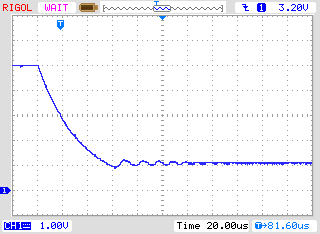
\includegraphics[width=9cm]{../PNG/AREF2_1V.png}
    \caption{� \(5~V\) �� \(1,1~V\)}
    \label{pic:aref1}
  \end{subfigure}
  ~
  \begin{subfigure}[b]{9cm}
    \centering
    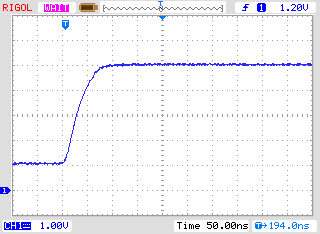
\includegraphics[width=9cm]{../PNG/AREF2VCC.png}
    \caption{� \(1,1~V\) �� \(5~V\)}
    \label{pic:aref5}
  \end{subfigure}
  \caption{������������ AREF � �������� \(1~nF\)}
\end{figure}


�������������� ��������� ����� ���� ����������� � ������ transistortester.h � config.h. ���� config.h  
�������� ���������� ���������� � ���������� ����/������� � �������� ���������, ������� ������������ ��� ���������. ���� 
transistortester.h ���������� ��������� ��� ��������� ����� �����������������, �������� � ������� ���. ������ ��� 
������������� �������� ��� ��������.


\chapter{Beschreibung des Messverfahrens}
\label{sec:measurement}
Ein vereinfachtes Schaltbild eines Eingangs-/Ausgangs-Pin des ATmega wird in Abbildung~\ref{fig:port} gezeigt.
Der Schalter PUD schaltet die Versorgung für alle ,,Pull Up''-Widerstände des ATmega ab.
Mit dem Schalter DD kann der Ausgang abgeschaltet werden, der Eingang funktioniert sowohl im Ausgabe- wie im
Eingabe-Modus. Im Eingabe-Modus wird mit dem Ausgabewert (PORT) der ,,Pull Up''-Widerstand des Eingangs mit geschaltet.
Die beiden Schalter PORT und DD können nicht gleichzeitig, sondern nur nacheinander geschaltet werden.
Weil beim Umschalten der ,,Pull Up''-Widerstand die Messung stören könnte, bevorzuge ich die komplette
Abschaltung aller ,,Pull Up''-Widerstände mit dem PUD-Schalter.
Natürlich sind die Schalter elektronisch und die Widerstände \(19\Omega\) und \(22\Omega\) sind angenäherte Werte.
\begin{figure}[H]
\centering

\includegraphics[]{../FIG/port.eps}
\caption{Vereinfachtes Schaltbild jedes ATmega-Portpins}
\label{fig:port}
\end{figure}

Jeder der drei Testpins Ihres TransistorTesters wird aus drei ATmega-Portpins gebildet,
was im vereinfachten Schaltbild des Testpins TP2 (mittlerer der drei Pins) in Abbildung~\ref{fig:terminal} gezeigt wird.

\begin{figure}[H]
\centering

\includegraphics[]{../FIG/terminal.eps}
\caption{Vereinfachtes Schaltbild des Testpins TP2}
\label{fig:terminal}
\end{figure}

Jeder Testpin (Messport) kann als digitaler oder analoger Eingang benutzt werden.
Diese Mess\-fähig\-keit ist un\-abhän\-gig von der Verwendung des Ports als Ausgang.
Jeder Testpin kann als Ausgang verwendet werden und in diesem Zustand mit GND (\(0V\)) oder VCC (\(5V\)) verbunden werden,
oder er kann über die Widerstände (\(680\Omega\) oder \(470k\Omega\)) mit entweder GND oder VCC verbunden werden.
Tabelle \ref{tab:case} zeigt alle denkbaren Messmöglichkeiten.
Beachten Sie, dass der positive Zustand durch direktes Verbinden mit VCC (Port C) oder
durch Verbinden mit dem \(680\Omega\) Widerstand mit VCC (Port B) erreicht werden kann.
Die gleiche Möglichkeit hat der negative Zustand des Testpins zu der GND-Seite.
Der Test-Zustand meint, dass der Pin offen sein kann (Eingang), verbunden über den \(470k\Omega\)-Widerstand
mit VCC oder GND, oder der Pin kann über den \(680\Omega\)-Widerstand mit VCC oder GND verbunden sein.

\begin{table}[H]
  \begin{center}
    \begin{tabular}{| l | c | c | c |}
    \hline
      & Zustand Pin 1 & Zustand Pin 2 & Zustand Pin 3 \\
    \hline
   1. & positiv    &  negativ   &  test \\
   2. & positiv    &  test      & negativ \\
   3. & test       &  negativ   & positiv \\
   4. & test       &  positiv   & negativ \\
   5. & negativ    &  test      & positiv \\
   6. & negativ    &  positiv   &  test  \\
    \hline
    \end{tabular}
  \end{center}
  \caption{alle Messmöglichkeiten}
  \label{tab:case} 
\end{table}

Wenn die Kondensatormessung des Testers konfiguriert ist, versucht der Tester vor allen Messungen erst einmal,
die Kondensatoren an allen Anschlusspins zu entladen. Wenn das nicht gelingt, also die Restspannung zu hoch bleibt,
wird das Entladen nach etwa 12 Sekunden mit der Meldung ,,Cell!'' abgebrochen. Dies kann auch dann vorkommen, wenn
gar kein Kondensator angeschlossen ist. Die Ursache kann in diesem Fall sein, dass die Entlade-Grenzspannung für diesen
ATmega zu niedrig gewählt ist. Man kann eine höhere Restspannung mit der Makefile-Option CAP\_EMPTY\_LEVEL wählen.


 %\newpage
\section{��������� ����������������� ���������}
������������ �������� ���������� �������� � ������������ �����������
������� (������ �����, ������ TriStatePin). TriStatePin ������������
�������� �� ����� ��������� ��������  ������� ��� ���������. ����
������������� ����� ������ ������������� �������� �������� �
��������� ��������������� � VCC. ������ ������������� ����� ������
������������� �������� ��������.
������������� ������� ������������ ����� �������� \(680~\Omega\) � GND.
��������� ������� ������������ �������
�� ���������� �� �������. �������, TriStatePin �� \(5~ms\) ������������
����� �������� \(680~\Omega\) �� � GND � ���������� ���������� �� �������������
�������. ����� TriStatePin ������������� �� ���� (������� ������
������� �������������) � ����� ���������� ���������� ��������������
�������������� ������. ����� �������������� ������ ����������� �����
�������� \(680~\Omega\) �� \(5~ms\) � VCC � ����� ���������� ���������� ��
�������������  �������. ���� ���������� ���������� ���� �������
���������� ���������, �� ��� ����� ����� ��������������, ���
����������. ����� ���������� ����� ���������� � ������������ TriStatePin.\\

���� ���������� �������������� �������������� ������ � ������������� 
����������� TriStatePin ���� ��� \(115~mV\), � � ������������ TriStatePin 
�� ���� \(100~mV\), ��������������, ��� ��� ���������� ����������.\\

� ���������� ������������, ������� ���������� �������� ��� ����������,
�� ����������� ���������� � ������ � ������������ �����.\\

��� �������� � ������ ������������ ����� �������� �������������
����������� ��������� ����������� ������������ � ����� �������
�������� ����� ����������, ��� ���������� ������������ (JFET).\\

����� ���������� �������������� ����� �� ����������� N-���������� JFET
��� N D-MOSFET � P-���������� JFET ��� P-D MOSFET. ������ MOSFET
����� ���� ���������� �� �������������� ���� ������� ��� �����
��������� TriStatePin.\\

����� �������� ��������� FET ����������� ����, �� �������� � ���������� \(680~\Omega\) � ������, 
��� �������� �� ������� \ref{fig:JFETcd} . ��� ��������� �������� ������ �������� ��������� ���� 
����������� ������� �� ������ ������, ������, ��� \(I_\mathrm{DSS}\) FET ����������� ����� �� ����� 
���� ���������� ��-�� ������������ �������� ������������� ��������� \(680~\Omega\).

\begin{figure}[H]
\centering

\includegraphics[]{../FIG/JFETcd.eps}
\caption{��������� ���������� ������-����� � ���� ������ N-JFET ����������� }
\label{fig:JFETcd}
\end{figure}

���� � �������� ��� ���� ����� ������������� � ������������� �������������� �������� ��� ������� �� TristatePin, 
�� ��������� � ������ �����������, ��������� �  ������� \ref{sec:pnp}.
���� ��� ��� ���������, �� ��������� ���� ������ � \ref{sec:diode} � ������.

\subsection{��������� P-N-P ����������� ��� P-Channel-MOSFET}
\label{sec:pnp}
������� �������� ����������� �������� ��������������� P-N-P ����������� � ����� � ����� ����������� 
(���������� �����������). ����� ��������� �������� �� ������� \ref{fig:pnpcc}.
���� ���������� ���� (\(UB\)) ���������� � ���������� \(680~\Omega\),  ���� \(9~mV\), �� ����������� 
�������� ����������� �� ������� \(hFE = \frac{UE-UB}{UB}\).
���������� \(UE\) ��� �������� ����� ����������� �� �������� � VCC. �������� ����� ����������� \(22~\Omega\) 
� \(19~\Omega\) �� �����������. ���� ���������� \(UB\) ���� \(10~mV\), ��������� ������ � ���������� \(470~k\Omega\) 
� ����. � ���� ������ �����������  
�������� ����������� �� ������� \(hFE = \frac{UE \cdot 470000}{UB \cdot (680+22)}\).

\begin{figure}[H]
\centering

\includegraphics[]{../FIG/PNPcc.eps}
\caption{��������� hFE P-N-P ����������� � ����� � ����� ����������� }
\label{fig:pnpcc}
\end{figure}

����� ������ ����� ��� ��������������� P-N-P ����������� � ����� � ����� ���������. ������������� ������� 
�������� ������ ���������� ����� � VCC, ������������� ������� ����� �������� \(680~\Omega\) ���������� � GND, 
��� �������� �� ������� \ref{fig:pnpce}. 
���� �� ������������� ������� �������� ���� ���������� ���� \(3,4~V\), ����� ������� �������� \(680~\Omega\) 
��������� � GND, ������ ���� ������� ��� P-N-P ���������� ��� P ��������� FET. ����� �� ��� - ����� ���� ����� 
����������� �� ���������� ����. ���� ���������� ���� ������ \(0,97~V\), ��� ������ ���� P-N-P ����������. ��� ����, 
����� �������� ����������� ��������, � ���� ���� ������ ��������� \(680~\Omega\) ���������� �������� \(470~k\Omega\).
����������� �������� ����������� �� ������� \(hFE = \frac{(UC-UC0) \cdot 470000}{UB \cdot (680+19)}\) .
���������� UC0 �������� ����������� �� ������������ ��������� ��� �������� ����. ��� ��������������, ���������� 
�������� ����� ������� ����������� ��������, ������������ ������ ��� ������ ��������. � ������ 1.08k ����������� 
�������� � ����� � ����� ��������� ������������ ������ ��� ����������������� ATmega328. ��� ������ ����������������� 
������������ ������ ����� � ����� �����������.\\

��������, ��������� ��� P-N-P �����������, ������������� ������, ���� ������� �������������� ���������. ����� 
������������� ����������� P-N-P ����������� � ��������� ��������� (��������� � ��������� �������� �������), 
��������� � ����� ������� ������������� �������� ��������� ����������. 
���� ���������� ���� ����, ��� \(0,97~V\), �� ��� ������ ���� P-E-MOS. � ���� ������ ��������� ���������� ������� 
���������� ��� ������� ������������ ������� � ���������� \(470~k\Omega\) �� VCC �� GND, ������ �� �������� ����� 
���������  �������  �����, � �����, ����������� ���������� �������.
\begin{figure}[H]
\centering

\includegraphics[]{../FIG/PNPce.eps}
\caption{��������� � ��������� hFE P-N-P ����������� � ����� � ����� ��������� }
\label{fig:pnpce}
\end{figure}

\subsection{��������� N-P-N ����������� ��� N-Channel-MOSFET}
��������� N-P-N ����������� ���������� ����� �� �������, ��� � P-N-P �����������, � ��������� ������������ �������� 
� ����� � ����� �����������.
������ ��������� ������� � ���������� � ���� ���� \(680~\Omega\) ������������ � VCC. ���� ���������� �� ��������� � 
���� ���� ������� �����, ������ \(680~\Omega\) ������ �������� \(470~k\Omega\).
����� ��������� ������������ � ����� � ����� ���������, ��� �������� �� ������� \ref{fig:npnce}.
���� ���������� ���������� ���� \(1,6~V\) � �������� � ���� ���� \(680~\Omega\) �������� � VCC, �� ��� ����� ���� N-P-N 
����������, N-��������� MOSFET ��� ��������/��������. �������� ��� �������� ����� ���� ���������������� ����� 
�������� �������. ���� �������� �� ����������� ������, ����������� � ������� \(10~ms\) � GND ����������, ��� � ����� 
������ ��������. ���� �������� ����� �������������� ���������� � GND �, �����, �������� ���������� � VCC, �������� 
�� ������ ����� ���������� (��� ����). ������ � ����, ��� ������ ����� ��������� ������ ���������� ���������, ������ 
��� ��� ��������� ����� ��������� ������ \(6~mA\). ���� ��� ����� ��������������� � ���������, �� ���������� ������� 
����� � �������� �����������, ����� ��������� ��� ����������� ��������. 
\begin{figure}[H]
\centering

\includegraphics[]{../FIG/NPNce.eps}
\caption{��������� � ��������� hFE N-P-N ����������� � ����� � ����� ��������� }
\label{fig:npnce}
\end{figure}
���� �� ��������, �� �������� �� ���� ������������, �� ��� ����� ���� N-P-N ���������� ��� N ��������� E-MOSFET. 
������� ���������� N-P-N ����������� ����� ������ � ���������� ��������, ����� �������, ���� ��� ����� ���� 
��������������� �����������. ����������� �������� � ����� � ����� ��������� ����������� �� ������� 
\(hFE = \frac{(VCC-UC-UC0)\cdot 470000}{(VCC-UB)\cdot (680+22)}\).
���� ���������� ���� ��� ������� ����������, �� � ���� ���� ���� ��� ��� �� ���, ������, ������� ����� N-���������  
E-MOS (MOSFET �����������). � ���� ������ ��������� ���������� ���������� ��� ������� ������������ ������� � 
���������� \(470~k\Omega\) �� VCC �� GND, ������ �� �������� ����� ��������� ������� �����, � ����� ����������� 
���������� �������. ��� ��������� �������� 11 ��� � ����������� ����������� ���, ��� �������� �� 
�������~\ref{fig:eleven}.
��������� ���������� �� 4 � ������� �� 9, ����� �������� ���������� � \(mV\).
\begin{figure}[H]
\centering
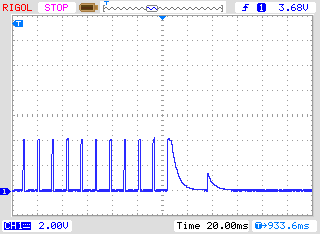
\includegraphics[]{../PNG/IRFU120gate.png}
\caption{��������� ���������� ���������� N-���������� MOSFET}
\label{fig:eleven}
\end{figure}

\subsection{���������� ����-����� ������������ ������������}

\begin{figure}[H]
\centering

\includegraphics[]{../FIG/CheckSemi1.eps}
\caption{����-����� ������������ ������������. ����� 1: JFET � D-MOS}
\label{fig:ChkSemi1}
\end{figure}

\begin{figure}[H]
\centering
\includegraphics[]{../FIG/CheckSemi2.eps}
\caption{����-����� ������������ ������������. ����� 2: BJT � E-MOS}
\label{fig:ChkSemi2}
\end{figure}

\begin{figure}[H]
\centering
\includegraphics[]{../FIG/CheckSemi3.eps}
\caption{����-����� ������������ ������������. ����� 3: �������� � ��������}
\label{fig:ChkSemi3}
\end{figure}


\subsection{��������� ������}
\label{sec:diode}
���� ���������������� ������� ����� ��������� ���, �� ������� ����� ������� ��� ����. ������� ���������� � 
���������� \(680~\Omega\) ������ ���� ����� \(0,15~V\) � \(4,64~V\). �������   ���������� � ���������� \(680~\Omega\) 
������ ���� � 1.125 ���� ������ ������� ���������� � ���������� \(470~k\Omega\) � �������  ���������� � 
���������� \(470~k\Omega\) ������ ���� � 16 ��� ������, 
��� �������  ���������� � ���������� \(680~\Omega\). �������������: ��� ������������� ��������� � 
���������� \(470~k\Omega\) ���������� ������ ���� �� ����, ��� � ���������� ��������� � 
���������� \(680~\Omega\).
� �������, ��� ���� ����� ������ �������������� ����. ��� ������������� ���� ������, ���������� ��������-�����������, 
���������� ����������� ���� ������ � ��������������� �����������. ���� ��������� ������ ��������� ����, �� ��� 
������ � �������� ����������� ���������� � ���������� \(470~k\Omega\) ������������ � VCC. ���������� ����� \(2~nA\).
���� ���  ������ ������ \(5,3~\mu A\) (���������� �� ��������� \(470~k\Omega\) ���������� ������ ��� \(2,5~V\)), 
��������� ������������ � ���������� \(680~\Omega\).
� ���� ������ ���������� ������ ����� \(1~\mu A\).
����� ����, ��� ���������� �����, ����� ���� �������� ������� � �������� �����������.

\subsection{���������� ��������� ���������}
��������� ������� ���������� ���������� ������������� ������������ � ���������� ������������������ 
ATmega8, ATmega168, ATmega328.

\begin{table}[H]
  \begin{center}
    \begin{tabular}{| l | c | c | c |}
    \hline
   ��� ����� & Mega8@8MHz & Mega168 @8MHz & Mega328 @8MHz \\                
    \hline
    \hline
1N4148     & Diode, 715mV,        & Diode, 718mV,            & Diode, 715mV,           \\
           &               1pF    &               0pF, 2nA   &               1pF, 4nA  \\
    \hline
1N4150     & Diode, 665mV,        & Diode, 672mV,            & Diode, 666V,           \\
           &               1pF    &               1pF, 4nA   &              2pF, 6nA  \\
    \hline
BA157      & Diode, 619mV,        & Diode, 621V,              & Diode, 615mV,            \\
           &               19pF   &              17pF, 12nA   &               18pF, 12nA \\
    \hline
BY398      & Diode, 538mV,        & Diode, 541mV,             & Diode, 537mV,            \\
           &               16pF   &               14pF, 63nA  &               15pF, 63nA \\
    \hline
1N4007     & Diode, 650mV,        & Diode, 655mV,            & Diode, 650mV,           \\
           &               13pF   &               10pF, 6nA  &               13pF, 6nA \\
    \hline
LED green  & Diode, 1,96V, 5pF    & Diode, 1,95V, 4pF   & Diode, 1.95V, 4pF \\
    \hline
ZPD2,7     & 2xDi, 743mV, 2,53V   & 2xDi, 737mV, 2,52V  & 2xDi, 733mV, 2,51V \\
    \hline
BU508A B+E & Diode, 609mV,        & Diode, 611mV,                & Diode, 606mV,              \\
           &               5,15nF &               5,20nF, 0,39uA &               5,25nF, 0,4uA\\
    \hline
BU508A B+C & Diode, 582mV,        & Diode, 586mV,             & Diode, 587mV,            \\
           &               256pF  &               255pF, 21nA &               259pF, 19nA\\
    \hline
AC128 B+E  & Diode, 272mV,        & Diode, 277mV,              & Diode, 273mV,             \\
           &               0pF    &               0pF, 2,2uA   &               0pF, 2,3uA  \\
    \hline
AC128 B+E  &                      &                     & Diode, 349mV,               \\
� �����������     &                      &                     &               140pF, 0,57uA \\
    \hline
MBR20100CT & 2xDi, 337mV, 337mV   & 2xDi, 338mV, 338mV  & 2xDi, 336mV, 335mV  \\
    \hline
MBR20100CT & Diode, 337mV,        & Diode, 339mV,             & Diode, 337mV,            \\
           &               345pF  &               351pF, 29nA &               350pF, 25nA\\
    \hline
MBR4045PT  & Diode, 243mV,        & Diode, 233mV,               & Diode, 235mV,              \\
� �����������     &               1,80nF &               1,94nF, 1,7uA &               1,95nF, 1,8uA\\
    \hline
SK14       & Diode,    mV,        & Diode,    mV,               & Diode, 263mV,              \\
           &                  0pF &                   pF,    nA &               0pF, 0,57uA\\
    \hline
SK14       & Diode,    mV,        & Diode,    mV,               & Diode, 334mV,              \\
� �����������     &                   nF &                   pF,    nA &               88pF, 4nA\\
    \hline
SF38G      & Diode, 519mV,        & Diode, 521mV,            & Diode, 516mV,            \\
           &               107pF  &               105pF, 2nA &               106pF, 2nA \\
    \hline
    \end{tabular}
  \end{center}
  \caption{���������� ��������� ������}
  \label{tab:diodes} 
\end{table}

��������� �������� ������� ��� �������� ����� MBR4045PT �������� ������ � �����������. 
��� ������� ������� ����� ������ ����� \(40~A\) �����. ����� �������� ������� �������� ����-������� 
������������ ����������� AC128 ����� ���� �������� ������ � �����������.

\begin{table}[H]
  \begin{center}
    \begin{tabular}{| l | c | c | c | c | c |}
    \hline
             ��� & ��� & Mega8           & Mega328        & Mega328         & Mega328 \\
�����������     & ��-��     & �����         &                & �����         & ����� \\
            &     & ���������      &                & ���������       & ������� \\
    \hline
    \hline
BU508A      & NPN & \(\beta\)=9, 601mV      &  \(\beta\)=9, 597mV    &   \(\beta\)=9, 598mV    & \(\beta\)=4, 484mV \\
    \hline
2N3055      & NPN & \(\beta\)=20, 557mV     &  \(\beta\)=21, 550mV   &   \(\beta\)=21, 550mV   & \(\beta\)=6, 442mV \\
    \hline
BC639       & NPN & \(\beta\)=148, 636mV    &  \(\beta\)=172, 629mV  &   \(\beta\)=172, 629mV  & \(\beta\)=158, 605mV \\
    \hline
BC640       & PNP & \(\beta\)=226, 650mV    &  \(\beta\)=176, 609mV  &   \(\beta\)=171, 655mV  & \(\beta\)=177, 608mV \\
    \hline
BC517       & NPN & \(\beta\)=23,9k, 1,23V  &  \(\beta\)=24,8k, 1,22V&   \(\beta\)=25,1k, 1,22V & \(\beta\)=764, 1,23V \\
    \hline
BC516       & PNP & \(\beta\)=75,9k, 1,21V  &  \(\beta\)=76,2k, 1,20V&   \(\beta\)=76,2k, 1,20V & \(\beta\)=760, 1,23V \\
    \hline
BC546B      & NPN & \(\beta\)=285, 694mV    &  \(\beta\)=427, 687mV  &   \(\beta\)=427, 687mV   & \(\beta\)=369, 683mV \\
    \hline
BC556B      & PNP & \(\beta\)=304, 704mV    &  \(\beta\)=254, 668mV  &   \(\beta\)=235, 709mV   & \(\beta\)=255, 668mV \\
    \hline
AC128 (Ge.) & PNP & \(\beta\)=63, 191mV     &  \(\beta\)=59, 191mV   &   \(\beta\)=57, 193mV    & \(\beta\)=43, 117mV \\
    \hline
BUL38D      & NPNp & \(\beta\)=37, 627mV    &  \(\beta\)=41, 617mV  &   \(\beta\)=40, 624mV     & \(\beta\)=36, 562mV \\
parasitic   & PNPn & \(\beta\)=11, 654mV    &  \(\beta\)=81, 543mV  &   \(\beta\)=10, 656mV     & \(\beta\)=83, 541mV \\
    \hline
BRY55/200   & Thyrist. &  0,84V     &  0,81V         &   0,81V          &  0,82V \\
    \hline
MAC97A6     & Triac    &  0,92V     &  0,90V         &   0,90V          &  0,90V \\
    \hline
    \end{tabular}
  \end{center}
  \caption{���������� ��������� ���������� ������������}
  \label{tab:bipolar} 
\end{table}

��������� ���������� ����������� ���������� �� �����������, ���������� � ����� ������ ������� ������������ 
����������� �� Markus F. ��������, ���������� ����������� BC517 ��� ������� ����� ������ ����������� 
������������: hFE=797 ������ 77200 � ���������� ����-������� = \(1438~mV\). ��� ������� �������������� ���������� 
������������ �������� � ����� � ����� �����������. ����� ����, ����� ������ ������������ ����������� ���������� 
����� �� ������ ��������� hFE � ����� � ����� ���������, ��� ����� ������� � ��������� ������� 
������� \ref{tab:bipolar}.
���������� ����-������� �������� ��� ��������� ����. ������ ���������� ����-������� ���������� ��� ���� ��������� 
������������ �������� (\(1,20~V\)). NPN-���������� BUL38D ����� ����� ����������� � ��������� ���������� �������� ����, 
������� ����� �������������� ����������� ����������� PNP-����������� � ����� �� ����� ���������� ����������� 
NPN �����������. � ������ ������������ ����������� 1.10k ��� ����������� �������������� � ���������� ����������� 
������� �. ���������� ���������� ����� ������ ��� ��������� ������� �������� ���� - �������. ��������������, 
��� ���������� ���������� ����� ����� ������� ������� ��������. ���� ������ � ���������� ������� ������� �� ����� 
������ ���������� ���������, �� ����� �������� ��������� ����������� �����������. ������� ����������� ����������� 
����� �������� �������� n (PNPn). ���������� ���������� ������������ ������ � �������� ������, ������������� �� 
��� �� ���������, ��� � ���������� ����������, � �� � ������� ������.\\

��������� ������� \ref{tab:germanium} ���������� ���������� ��������� ��� ����������� ������������, ������� �������� 
����������� ��-�� ������������� ����������� � �������� ��������� ���� ����������. ������������ ������ ���������� 
������������ ������ �� Markus F. � ���������� ������ 1.10k. ������ 1.10k ��� ATmega328 �������� ����������� �������� 
� ������ � ����� ����������� � ����� ��������� � ������ ��������� ���� ����������, � ������� ����� ������� ���������. 
�������� ��� ���������� �� ���������� � ����� ������ ������� ������������ �����������.

\begin{table}[H]
  \begin{center}
    \begin{tabular}{| l | c | c | c |}
    \hline
      ��� & Mega8@1MHz          & Mega168 @8MHz       & Mega328 @8MHz    \\
 �����������    & ������������ ���.    & ������ 1.10k       & ������ 1.10k  \\
            & Markus F.           &                     &        \\
    \hline
    \hline
AC128       & PNP, \(\beta\)=52, 279mV    & PNP, \(\beta\)=59, 184mV    & PNP, \(\beta\)=59, 191mV    \\
    \hline
AC116-65    & PNP, \(\beta\)=505, 378mV   & PNP, \(\beta\)=72, 146mV    & PNP, \(\beta\)=72, 149mV    \\
    \hline
AC116-145   & PNP, \(\beta\)=485, 294mV   & PNP, \(\beta\)=146, 161mV    & PNP, \(\beta\)=146, 163mV   \\
    \hline
AC176-65    & NPN, \(\beta\)=98, 235mV    & NPN, \(\beta\)=58, 94mV    & NPN, \(\beta\)=56, 96mV     \\
    \hline
GC122       & PNP, \(\beta\)=84, 368mV    & PNP, \(\beta\)=55, 117mV    & PNP, \(\beta\)=56, 117mV    \\
    \hline
GC301       & PNP, \(\beta\)=48, 289mV    & PNP, \(\beta\)=39, 184mV    & PNP, \(\beta\)=39, 188mV    \\
    \hline
AD161       & NPN, \(\beta\)=360, 230mV   & NPN, \(\beta\)=296, 126mV   & NPN, \(\beta\)=298, 128mV    \\
    \hline
AD162       & PNP, \(\beta\)=2127, 280mV  & PNP, \(\beta\)=89, 107mV    & PNP, \(\beta\)=89, 107mV    \\
    \hline
    \end{tabular}
  \end{center}
  \caption{���������� ��������� ����������� ���������� ������������}
  \label{tab:germanium}
\end{table}

� ������� \ref{tab:mos} �������� ���������� ��������� ��������� ������� ������������. ����� �� ���������� ���������� 
E-MOS ������������ �������� ���������� ������-�����, ������� ���������� �� ��������� ��������� ��������� ����� ATmega, 
������������� 
� ����� ����� �������� \(680~\Omega\).
��-�� ��������� ������� �������, ���������� �� ��� ����������
����� ������, ��� ��������� �������� �������� ����� ����������. ��������, � ����������� BS250 ��� ����������
���������� �� \(2,6~V\) �� \(2,5~V\), ��� ����������� ��������������� ������������ ��������
\(10~nF\) ����������� ������� ������ � �����.
������ ���������� ���������� �������� �������� ������� �������.
������� ������� ���������� ����� ������������ ������ ������ � ������� �� GND.
��������� ���������� \(5~V\) �� ������� ������� �������� ������������� ��� ��������� ������������ ����
��� ��������� IGBT. ��� ������ ����������� �����������.
� ����������� ������� �������������� ������ �������� ���� ���������-�������.
��������, ��������, \(3~V\), ������������ � ������, ����� ������ �������� � ������������.
������ ����� ��������� ������ ���� ��������� � ��������� ������ (TP) ������� ������ ���������� �������.
��� ���������� ���������� ������� ������ ������ ���������� IGBT.
������������ ���������� ������������ ������-���� ������ ���� ��������� �� �������� ���������� �������,
����� �������� ���������� ���������� ������������.
��� JFET ������������ � �������� �������������� ����� �������� ��� Idss,
���������� ����� ����� ��� ���������� ������-����� ������ \(0~V\). � ������ ����������, ������, ��� �� �����
��������� ��������, ������������ �������������� �������� � ����� JFET ��������� \(680~\Omega\).
����������� �������� ���������� �������� ���������� Vgs, ������� ����� ������������ �� ����������.
� ����������� ���������� \(470~k\Omega\) � ���� ������ JFET ��� �����-���� ����� ����� �������.
����� �������, ���������� ������� Vgs\_off �����-������ ����� ���� ���������� ���������� �����,
��� �������, ��� ��� �� �������� \(5~V\).
� ����� ����� �������� ������� �� ����� ���������� ��� ������-����� Igss � ����� ������������������ ���������.
���� ��������� ��� ������ \(40~mA\), ������������� ���������� ��������� ��� ������������� � ���� ������.
�� ����� �������� ���������� �� ������ ������ ��� ��������� �� ����� ��������� �������������� �������� ����.
��������� ��� ���������� ���������, ����� ��������� ��� ������-����� Idss,
��� ���� �� �� ������ ��������� �������� \(40~mA\).
��-�� ������������ ����������� ������������ JFET, ���������� �������� ���� �� ������.


\begin{table}[H]
  \begin{center}
    \begin{tabular}{| l | c | c | c | c |}
    \hline
 ����������  &  ���    & Mega8@8MHz       & Mega168 @8MHz    & Mega328 @8MHz \\
             &         &                  &                  &               \\
    \hline
    \hline
ZVNL120A     & N-E-MOS & D, 1,6V, 147pF   & D, 1,5V,141pF    & D, 1,5V, 140pF \\
    \hline
IRF530N      & N-E-MOS & D, 3,6V, 1.55nF  & D, 3,6V, 1,54nF  & D, 3,6V, 1,54nF \\
    \hline
BS170        & N-E-MOS & D, 2,6V, 78pF    & D, 2,6V, 68pF    & D, 2,6V, 68pF \\
    \hline
IRL3803      & N-E-MOS & D, 2,3V, 9.81nF  & D, 2,3V, 9,71nF  & D, 2,3V, 9,74nF \\
    \hline
IRFU120N     & N-E-MOS & D, 4,2V, 909pF   & D, 4,2V, 913pF   & D, 4,2V, 911pF \\
    \hline
BUZ71A       & N-E-MOS & D, 3,2V, 714pF   & D, 3,2V, 708pF   & D, 3,2V, 705pF \\
    \hline
ZVP2106A     & P-E-MOS & D, 3,2V, 122pF   & D, 3,2V,115pF    & D, 3,2V, 116pF \\
    \hline
IRF5305      & P-E-MOS & D, 3,6V, 2.22nF  & D, 3,6V, 2,22nF  & D, 3,6V, 2,22nF \\
    \hline
BS250        & P-E-MOS & D, 2,6V, 53pF    & D, 2,6V, 43pF    & D, 2,6V, 44pF \\
    \hline
IRFU9024     & P-E-MOS & D, 3,5V, 937pF   & D, 3,6V, 945pF   & D, 3,5V, 933pF \\
    \hline
J310         & N-JFET  & 3.1mA Vgs=2.2V   & 3.1mA Vgs=2.2V   & 3.1mA Vgs=2.2V \\
Idss=24-60mA &         &                  &                  & Idss=35mA      \\
    \hline
2N5459       & N-JFET  & 2.1mA Vgs=1.5V   & 2.1mA Vgs=1.5V   & 2.1mA Vgs=1.5V \\
Idss=4-16mA &          &                  &                  & Idss=8.2mA     \\
    \hline
BF256C       & N-JFET  & 3.4mA Vgs=2.4V   & 3.4mA Vgs=2.4V   & 3.4mA Vgs=2.4V \\
Idss=11-18mA &         &                  &                  & Idss=14mA      \\
    \hline
BF245A       & N-JFET  & 1.1mA Vgs=.75V   & 1.1mA Vgs=0.75V  & 1.1mA Vgs=0.75V \\
Idss=2-6mA   &         &                  &                  & Idss=3.6mA      \\
    \hline
BF245B       & N-JFET  & 2.5mA Vgs=1.7V   & 2.5mA Vgs=1.7V   & 2.5mA Vgs=1.7V \\
Idss=6-15mA  &         &                  &                  & Idss=10mA      \\
    \hline
BF245C       & N-JFET  & 3.9mA Vgs=2.7V   & 3.9mA Vgs=2.7V   & 3.9mA Vgs=2.7V \\
Idss=12-25mA &         &                  &                  & Idss=17mA    \\
    \hline
J175        & P-JFET   & 3.2mA Vgs=2.2V   & 3.2mA Vgs=2.2V   & 3.2mA Vgs=2.2V \\
Idss=7-60mA &          &                  &                  & Idss=26mA      \\
    \hline
2N5460      & P-JFET   & 0.78mA Vgs=0.54V & 0.77mA Vgs=0.54V & 0.78mA Vgs=0.54V \\
Idss=1-5mA  &          &                  &                  & Idss=2.6mA       \\
    \hline
BSS169      & N-D-MOS   & 2,6mA Vgs=1,8V & D, 2,6mA Vgs=1,8V & D, 2,6mA Vgs=1,8V \\
    \hline
GP07N120    & N-E-IGBT & C=3,81nF Vt=4,2V & C=3,76nF Vt=4,2V & C=3,74nF Vt=4,2V \\
    \hline
G4PC30      & N-E-IGBT &                  &                  & C=2.22nF         \\
� ��������  &          &                  &                  & Vt=2.0V+3.2V \\
    \hline
    \end{tabular}
  \end{center}
  \caption{���������� ��������� ���-������������}
  \label{tab:mos} 
\end{table}

 %\newpage
\section{��������� ����������}
������ �������� ������� �������� ���������� ������ ��������� � ����� ����������� ����. ��� �� �����  �������� 
����� ������� ���� �� ������ �������� ������ ��������� � ������ ����������� ����. ��������� � ��������������� 
����������� ������������ ������ ��� ����, ����� ���������������� ��������. ���� �������������� ����� ������ 
����������� ������� �������, �� ��� �� ��������.

\subsection{��������� ��������� � ����������� 680 ��}
��������� ������������ ��������� Rx �������������� ����� ��������� � �������������� ������������ ����������
 \(680~\Omega\). ���������� ����� ����� ��������� ��� ������������� ������� 1 (TP1) � 3 (TP3) �������� �� 
��������~\ref{fig:RL1mes} �~\ref{fig:RL2mes} ��� ������ ����� ��������� ���������� ���������.

\begin{figure}[H]
\centering
\includegraphics[]{../FIG/ResistormessL1.eps}
\caption{��������� ���� 1 � ���������� \(680~\Omega\) }
\label{fig:RL1mes}
\end{figure}

\begin{figure}[H]
 \centering
 \includegraphics[]{../FIG/ResistormessL2.eps}
 \caption{��������� ���� 2 � ���������� \(680~\Omega\) }
\label{fig:RL2mes}
\end{figure}


� ����� ������� ���������� ������������� ����� 1, � ������ ������� - ������������� ����� 3. � ����� ���������� 
�� ������, ��� ����� 3 (������ �������) �������� � VCC, ����� 1 (����� �������) �������� � GND. ����������� ����, 
�������� ����� �������� Rx �������� ����������. ��������  ������, ������������� �� �����, �������� ������� ������, 
�������� ������, ������������ � �������� �����, ������������ ����� ������, �������������� ����� - ������. � ����� 
���������� ����� ��������� ��� ������ ���� ����������, ������ ��� ��������� �������� ���������� ����� VCC � GND 
��������� (���� ������������� ��������� ���������� � � ��������� ������). ������ ���������� ���������� �� 
����������, ������ ��� �������� ������������ ���������. 
������ V �� ��������� �������� �����, ������������ ��� ��������� ����������. � ����� ������������� �������� 
��������� Rx ����� ���� ��������� �� ��������� �������� ��������� � ����������� ����������, ���� ��������� 
��������� Rx � \(680~\Omega\) �� ������� ������. ������������� ���������� ���������� �������� �� 
�������~\ref{fig:RLvtot}, ��� �������� ��������� �������� � ��������������� ��������.
\begin{figure}[H]
\centering
% GNUPLOT: LaTeX picture with Postscript
\begingroup
  \makeatletter
  \providecommand\color[2][]{%
    \GenericError{(gnuplot) \space\space\space\@spaces}{%
      Package color not loaded in conjunction with
      terminal option `colourtext'%
    }{See the gnuplot documentation for explanation.%
    }{Either use 'blacktext' in gnuplot or load the package
      color.sty in LaTeX.}%
    \renewcommand\color[2][]{}%
  }%
  \providecommand\includegraphics[2][]{%
    \GenericError{(gnuplot) \space\space\space\@spaces}{%
      Package graphicx or graphics not loaded%
    }{See the gnuplot documentation for explanation.%
    }{The gnuplot epslatex terminal needs graphicx.sty or graphics.sty.}%
    \renewcommand\includegraphics[2][]{}%
  }%
  \providecommand\rotatebox[2]{#2}%
  \@ifundefined{ifGPcolor}{%
    \newif\ifGPcolor
    \GPcolortrue
  }{}%
  \@ifundefined{ifGPblacktext}{%
    \newif\ifGPblacktext
    \GPblacktexttrue
  }{}%
  % define a \g@addto@macro without @ in the name:
  \let\gplgaddtomacro\g@addto@macro
  % define empty templates for all commands taking text:
  \gdef\gplbacktext{}%
  \gdef\gplfronttext{}%
  \makeatother
  \ifGPblacktext
    % no textcolor at all
    \def\colorrgb#1{}%
    \def\colorgray#1{}%
  \else
    % gray or color?
    \ifGPcolor
      \def\colorrgb#1{\color[rgb]{#1}}%
      \def\colorgray#1{\color[gray]{#1}}%
      \expandafter\def\csname LTw\endcsname{\color{white}}%
      \expandafter\def\csname LTb\endcsname{\color{black}}%
      \expandafter\def\csname LTa\endcsname{\color{black}}%
      \expandafter\def\csname LT0\endcsname{\color[rgb]{1,0,0}}%
      \expandafter\def\csname LT1\endcsname{\color[rgb]{0,1,0}}%
      \expandafter\def\csname LT2\endcsname{\color[rgb]{0,0,1}}%
      \expandafter\def\csname LT3\endcsname{\color[rgb]{1,0,1}}%
      \expandafter\def\csname LT4\endcsname{\color[rgb]{0,1,1}}%
      \expandafter\def\csname LT5\endcsname{\color[rgb]{1,1,0}}%
      \expandafter\def\csname LT6\endcsname{\color[rgb]{0,0,0}}%
      \expandafter\def\csname LT7\endcsname{\color[rgb]{1,0.3,0}}%
      \expandafter\def\csname LT8\endcsname{\color[rgb]{0.5,0.5,0.5}}%
    \else
      % gray
      \def\colorrgb#1{\color{black}}%
      \def\colorgray#1{\color[gray]{#1}}%
      \expandafter\def\csname LTw\endcsname{\color{white}}%
      \expandafter\def\csname LTb\endcsname{\color{black}}%
      \expandafter\def\csname LTa\endcsname{\color{black}}%
      \expandafter\def\csname LT0\endcsname{\color{black}}%
      \expandafter\def\csname LT1\endcsname{\color{black}}%
      \expandafter\def\csname LT2\endcsname{\color{black}}%
      \expandafter\def\csname LT3\endcsname{\color{black}}%
      \expandafter\def\csname LT4\endcsname{\color{black}}%
      \expandafter\def\csname LT5\endcsname{\color{black}}%
      \expandafter\def\csname LT6\endcsname{\color{black}}%
      \expandafter\def\csname LT7\endcsname{\color{black}}%
      \expandafter\def\csname LT8\endcsname{\color{black}}%
    \fi
  \fi
  \setlength{\unitlength}{0.0500bp}%
  \begin{picture}(7200.00,5040.00)%
    \gplgaddtomacro\gplbacktext{%
      \csname LTb\endcsname%
      \put(1078,704){\makebox(0,0)[r]{\strut{} 0}}%
      \csname LTb\endcsname%
      \put(1078,1518){\makebox(0,0)[r]{\strut{} 1000}}%
      \csname LTb\endcsname%
      \put(1078,2332){\makebox(0,0)[r]{\strut{} 2000}}%
      \csname LTb\endcsname%
      \put(1078,3147){\makebox(0,0)[r]{\strut{} 3000}}%
      \csname LTb\endcsname%
      \put(1078,3961){\makebox(0,0)[r]{\strut{} 4000}}%
      \csname LTb\endcsname%
      \put(1078,4775){\makebox(0,0)[r]{\strut{} 5000}}%
      \csname LTb\endcsname%
      \put(1210,484){\makebox(0,0){\strut{}100m}}%
      \csname LTb\endcsname%
      \put(2142,484){\makebox(0,0){\strut{}1 }}%
      \csname LTb\endcsname%
      \put(3074,484){\makebox(0,0){\strut{}10 }}%
      \csname LTb\endcsname%
      \put(4007,484){\makebox(0,0){\strut{}100 }}%
      \csname LTb\endcsname%
      \put(4939,484){\makebox(0,0){\strut{}1k}}%
      \csname LTb\endcsname%
      \put(5871,484){\makebox(0,0){\strut{}10k}}%
      \csname LTb\endcsname%
      \put(6803,484){\makebox(0,0){\strut{}100k}}%
      \put(176,2739){\rotatebox{-270}{\makebox(0,0){\strut{}voltage / mV}}}%
      \put(4006,154){\makebox(0,0){\strut{}resistor Rx / Ohm}}%
      \put(4006,4665){\makebox(0,0){\strut{}}}%
      \put(286,110){\makebox(0,0)[l]{\strut{}}}%
    }%
    \gplgaddtomacro\gplfronttext{%
      \csname LTb\endcsname%
      \put(3594,3094){\makebox(0,0)[r]{\strut{}PC2, type 1}}%
      \csname LTb\endcsname%
      \put(3594,2874){\makebox(0,0)[r]{\strut{}PC0, type 2}}%
    }%
    \gplbacktext
    \put(0,0){\includegraphics{../GNU/RLvtot}}%
    \gplfronttext
  \end{picture}%
\endgroup

\caption{���������� ��� ���������� ���� 1 � ���� 2 � ���������� \(680~\Omega\) }
\label{fig:RLvtot}
\end{figure}
������  ��������� ���� 1 �������  ��  �������~\ref{fig:RLvlow} � ���������� ��������� ����������� ��� ����� 
�������� ����������. ����� �����, ��� ��� ��������� ������� ��������� �������� ��������� ���� \(2~\Omega\)
���������� ������ ���������� ���, ��� ����������� ���������� \(4,9~mV\) � \(5~V\) ���.  ���� ������ 3 ������� 
��� �� \(0~\Omega\) �� \(2~\Omega\).
����� AUTO\_SCALE\_ADC, ������������� �������� ���, ����� ������ � ���� ������. ��� �� ����� ������� � ���������� 
��������� ����������� ��������� ��������� ���� 2 ������� �� �������~\ref{fig:RLvhigh}.
� ���������, �� �� ����� ������������ ������� ���������� ��� ��� ��������� ����~2 � ���� ���������, ������ ��� 
���������� ������� ������, � � ����������� ATmega ��� ����������������� ����� ���. ��������� � 
����������� \(680~\Omega\) ���������� ��� ��������� ���������� ��������� �� \(20~k\Omega\)
(���������� ���������� ����~2 ����� ���� \(169~mV\)).

��� ����� ������� �������� ����������� ��������� ���������  ���������� � ����������� \(470~k\Omega\). ���� ��� 
����� ��������������� � ���, ��� ��� �� ������ ��� ��������, �� ���������� �������� ����� ��������� ������� � 
�������� �������� ������������� ��������� ��� ����������� �� �������. ���� ������� ����� AUTO\_SCALE\_ADC, � 
���� �� ���������� ����� ����� ��������� ���� \(0,98~V\), ���������� ������� �������� ��������� � ������������� 4 
��� ���� ��������. ������ ���������� �������� ����� ����������� 1. ��� ������� ��� ����, ����� ����������� 
����������� 4 ��� ������� ���������� ����� ���������. ����������� 4 ���� ������ ��� ����������������� ATmega168 
� ATmega328, ��� ATmega8 � �������� �������� ������������ ����� 2, ���� ���������� ���� \(0.98~V\), ������ ��� ������� 
���������� ��� ��� ATmega8 \(2,54~V\) ������ \(1,1~V\) ��� ATmega168 � ATmega328. ��� ATmega168 � ATmega328 ��������� 
���������� �� ���������� ����� ���������, ���� �� ����������� ������� ��������� ��� ���������� ����� �������. 
��� ������������� ����� ������ ������� ������������ ����� �� ������������, ��� ���������, �� ������, � 
������������� ����������� ���� ������� ������� ������������� ����� �������� ���������.


\begin{figure}[H]
  \begin{subfigure}[b]{9cm}
    \centering
    \resizebox{9cm}{!}{% GNUPLOT: LaTeX picture with Postscript
\begingroup
  \makeatletter
  \providecommand\color[2][]{%
    \GenericError{(gnuplot) \space\space\space\@spaces}{%
      Package color not loaded in conjunction with
      terminal option `colourtext'%
    }{See the gnuplot documentation for explanation.%
    }{Either use 'blacktext' in gnuplot or load the package
      color.sty in LaTeX.}%
    \renewcommand\color[2][]{}%
  }%
  \providecommand\includegraphics[2][]{%
    \GenericError{(gnuplot) \space\space\space\@spaces}{%
      Package graphicx or graphics not loaded%
    }{See the gnuplot documentation for explanation.%
    }{The gnuplot epslatex terminal needs graphicx.sty or graphics.sty.}%
    \renewcommand\includegraphics[2][]{}%
  }%
  \providecommand\rotatebox[2]{#2}%
  \@ifundefined{ifGPcolor}{%
    \newif\ifGPcolor
    \GPcolortrue
  }{}%
  \@ifundefined{ifGPblacktext}{%
    \newif\ifGPblacktext
    \GPblacktexttrue
  }{}%
  % define a \g@addto@macro without @ in the name:
  \let\gplgaddtomacro\g@addto@macro
  % define empty templates for all commands taking text:
  \gdef\gplbacktext{}%
  \gdef\gplfronttext{}%
  \makeatother
  \ifGPblacktext
    % no textcolor at all
    \def\colorrgb#1{}%
    \def\colorgray#1{}%
  \else
    % gray or color?
    \ifGPcolor
      \def\colorrgb#1{\color[rgb]{#1}}%
      \def\colorgray#1{\color[gray]{#1}}%
      \expandafter\def\csname LTw\endcsname{\color{white}}%
      \expandafter\def\csname LTb\endcsname{\color{black}}%
      \expandafter\def\csname LTa\endcsname{\color{black}}%
      \expandafter\def\csname LT0\endcsname{\color[rgb]{1,0,0}}%
      \expandafter\def\csname LT1\endcsname{\color[rgb]{0,1,0}}%
      \expandafter\def\csname LT2\endcsname{\color[rgb]{0,0,1}}%
      \expandafter\def\csname LT3\endcsname{\color[rgb]{1,0,1}}%
      \expandafter\def\csname LT4\endcsname{\color[rgb]{0,1,1}}%
      \expandafter\def\csname LT5\endcsname{\color[rgb]{1,1,0}}%
      \expandafter\def\csname LT6\endcsname{\color[rgb]{0,0,0}}%
      \expandafter\def\csname LT7\endcsname{\color[rgb]{1,0.3,0}}%
      \expandafter\def\csname LT8\endcsname{\color[rgb]{0.5,0.5,0.5}}%
    \else
      % gray
      \def\colorrgb#1{\color{black}}%
      \def\colorgray#1{\color[gray]{#1}}%
      \expandafter\def\csname LTw\endcsname{\color{white}}%
      \expandafter\def\csname LTb\endcsname{\color{black}}%
      \expandafter\def\csname LTa\endcsname{\color{black}}%
      \expandafter\def\csname LT0\endcsname{\color{black}}%
      \expandafter\def\csname LT1\endcsname{\color{black}}%
      \expandafter\def\csname LT2\endcsname{\color{black}}%
      \expandafter\def\csname LT3\endcsname{\color{black}}%
      \expandafter\def\csname LT4\endcsname{\color{black}}%
      \expandafter\def\csname LT5\endcsname{\color{black}}%
      \expandafter\def\csname LT6\endcsname{\color{black}}%
      \expandafter\def\csname LT7\endcsname{\color{black}}%
      \expandafter\def\csname LT8\endcsname{\color{black}}%
    \fi
  \fi
  \setlength{\unitlength}{0.0500bp}%
  \begin{picture}(7200.00,5040.00)%
    \gplgaddtomacro\gplbacktext{%
      \csname LTb\endcsname%
      \put(946,704){\makebox(0,0)[r]{\strut{} 130}}%
      \csname LTb\endcsname%
      \put(946,995){\makebox(0,0)[r]{\strut{} 135}}%
      \csname LTb\endcsname%
      \put(946,1286){\makebox(0,0)[r]{\strut{} 140}}%
      \csname LTb\endcsname%
      \put(946,1576){\makebox(0,0)[r]{\strut{} 145}}%
      \csname LTb\endcsname%
      \put(946,1867){\makebox(0,0)[r]{\strut{} 150}}%
      \csname LTb\endcsname%
      \put(946,2158){\makebox(0,0)[r]{\strut{} 155}}%
      \csname LTb\endcsname%
      \put(946,2449){\makebox(0,0)[r]{\strut{} 160}}%
      \csname LTb\endcsname%
      \put(946,2740){\makebox(0,0)[r]{\strut{} 165}}%
      \csname LTb\endcsname%
      \put(946,3030){\makebox(0,0)[r]{\strut{} 170}}%
      \csname LTb\endcsname%
      \put(946,3321){\makebox(0,0)[r]{\strut{} 175}}%
      \csname LTb\endcsname%
      \put(946,3612){\makebox(0,0)[r]{\strut{} 180}}%
      \csname LTb\endcsname%
      \put(946,3903){\makebox(0,0)[r]{\strut{} 185}}%
      \csname LTb\endcsname%
      \put(946,4193){\makebox(0,0)[r]{\strut{} 190}}%
      \csname LTb\endcsname%
      \put(946,4484){\makebox(0,0)[r]{\strut{} 195}}%
      \csname LTb\endcsname%
      \put(946,4775){\makebox(0,0)[r]{\strut{} 200}}%
      \csname LTb\endcsname%
      \put(1078,484){\makebox(0,0){\strut{} 0}}%
      \csname LTb\endcsname%
      \put(1651,484){\makebox(0,0){\strut{} 1}}%
      \csname LTb\endcsname%
      \put(2223,484){\makebox(0,0){\strut{} 2}}%
      \csname LTb\endcsname%
      \put(2796,484){\makebox(0,0){\strut{} 3}}%
      \csname LTb\endcsname%
      \put(3368,484){\makebox(0,0){\strut{} 4}}%
      \csname LTb\endcsname%
      \put(3941,484){\makebox(0,0){\strut{} 5}}%
      \csname LTb\endcsname%
      \put(4513,484){\makebox(0,0){\strut{} 6}}%
      \csname LTb\endcsname%
      \put(5086,484){\makebox(0,0){\strut{} 7}}%
      \csname LTb\endcsname%
      \put(5658,484){\makebox(0,0){\strut{} 8}}%
      \csname LTb\endcsname%
      \put(6231,484){\makebox(0,0){\strut{} 9}}%
      \csname LTb\endcsname%
      \put(6803,484){\makebox(0,0){\strut{} 10}}%
      \put(176,2739){\rotatebox{-270}{\makebox(0,0){\strut{}voltage / mV}}}%
      \put(3940,154){\makebox(0,0){\strut{}resistor Rx / Ohm}}%
      \put(3940,4665){\makebox(0,0){\strut{}}}%
    }%
    \gplgaddtomacro\gplfronttext{%
      \csname LTb\endcsname%
      \put(5816,4602){\makebox(0,0)[r]{\strut{}PC2, type 1}}%
    }%
    \gplbacktext
    \put(0,0){\includegraphics{../GNU/RLvlow}}%
    \gplfronttext
  \end{picture}%
\endgroup
}
    \caption{��������� ���� 1}
    \label{fig:RLvlow}
  \end{subfigure}
  ~
  \begin{subfigure}[b]{9cm}
    \centering
    \resizebox{9cm}{!}{% GNUPLOT: LaTeX picture with Postscript
\begingroup
  \makeatletter
  \providecommand\color[2][]{%
    \GenericError{(gnuplot) \space\space\space\@spaces}{%
      Package color not loaded in conjunction with
      terminal option `colourtext'%
    }{See the gnuplot documentation for explanation.%
    }{Either use 'blacktext' in gnuplot or load the package
      color.sty in LaTeX.}%
    \renewcommand\color[2][]{}%
  }%
  \providecommand\includegraphics[2][]{%
    \GenericError{(gnuplot) \space\space\space\@spaces}{%
      Package graphicx or graphics not loaded%
    }{See the gnuplot documentation for explanation.%
    }{The gnuplot epslatex terminal needs graphicx.sty or graphics.sty.}%
    \renewcommand\includegraphics[2][]{}%
  }%
  \providecommand\rotatebox[2]{#2}%
  \@ifundefined{ifGPcolor}{%
    \newif\ifGPcolor
    \GPcolortrue
  }{}%
  \@ifundefined{ifGPblacktext}{%
    \newif\ifGPblacktext
    \GPblacktexttrue
  }{}%
  % define a \g@addto@macro without @ in the name:
  \let\gplgaddtomacro\g@addto@macro
  % define empty templates for all commands taking text:
  \gdef\gplbacktext{}%
  \gdef\gplfronttext{}%
  \makeatother
  \ifGPblacktext
    % no textcolor at all
    \def\colorrgb#1{}%
    \def\colorgray#1{}%
  \else
    % gray or color?
    \ifGPcolor
      \def\colorrgb#1{\color[rgb]{#1}}%
      \def\colorgray#1{\color[gray]{#1}}%
      \expandafter\def\csname LTw\endcsname{\color{white}}%
      \expandafter\def\csname LTb\endcsname{\color{black}}%
      \expandafter\def\csname LTa\endcsname{\color{black}}%
      \expandafter\def\csname LT0\endcsname{\color[rgb]{1,0,0}}%
      \expandafter\def\csname LT1\endcsname{\color[rgb]{0,1,0}}%
      \expandafter\def\csname LT2\endcsname{\color[rgb]{0,0,1}}%
      \expandafter\def\csname LT3\endcsname{\color[rgb]{1,0,1}}%
      \expandafter\def\csname LT4\endcsname{\color[rgb]{0,1,1}}%
      \expandafter\def\csname LT5\endcsname{\color[rgb]{1,1,0}}%
      \expandafter\def\csname LT6\endcsname{\color[rgb]{0,0,0}}%
      \expandafter\def\csname LT7\endcsname{\color[rgb]{1,0.3,0}}%
      \expandafter\def\csname LT8\endcsname{\color[rgb]{0.5,0.5,0.5}}%
    \else
      % gray
      \def\colorrgb#1{\color{black}}%
      \def\colorgray#1{\color[gray]{#1}}%
      \expandafter\def\csname LTw\endcsname{\color{white}}%
      \expandafter\def\csname LTb\endcsname{\color{black}}%
      \expandafter\def\csname LTa\endcsname{\color{black}}%
      \expandafter\def\csname LT0\endcsname{\color{black}}%
      \expandafter\def\csname LT1\endcsname{\color{black}}%
      \expandafter\def\csname LT2\endcsname{\color{black}}%
      \expandafter\def\csname LT3\endcsname{\color{black}}%
      \expandafter\def\csname LT4\endcsname{\color{black}}%
      \expandafter\def\csname LT5\endcsname{\color{black}}%
      \expandafter\def\csname LT6\endcsname{\color{black}}%
      \expandafter\def\csname LT7\endcsname{\color{black}}%
      \expandafter\def\csname LT8\endcsname{\color{black}}%
    \fi
  \fi
  \setlength{\unitlength}{0.0500bp}%
  \begin{picture}(7200.00,5040.00)%
    \gplgaddtomacro\gplbacktext{%
      \csname LTb\endcsname%
      \put(1078,704){\makebox(0,0)[r]{\strut{} 4780}}%
      \csname LTb\endcsname%
      \put(1078,995){\makebox(0,0)[r]{\strut{} 4785}}%
      \csname LTb\endcsname%
      \put(1078,1286){\makebox(0,0)[r]{\strut{} 4790}}%
      \csname LTb\endcsname%
      \put(1078,1576){\makebox(0,0)[r]{\strut{} 4795}}%
      \csname LTb\endcsname%
      \put(1078,1867){\makebox(0,0)[r]{\strut{} 4800}}%
      \csname LTb\endcsname%
      \put(1078,2158){\makebox(0,0)[r]{\strut{} 4805}}%
      \csname LTb\endcsname%
      \put(1078,2449){\makebox(0,0)[r]{\strut{} 4810}}%
      \csname LTb\endcsname%
      \put(1078,2740){\makebox(0,0)[r]{\strut{} 4815}}%
      \csname LTb\endcsname%
      \put(1078,3030){\makebox(0,0)[r]{\strut{} 4820}}%
      \csname LTb\endcsname%
      \put(1078,3321){\makebox(0,0)[r]{\strut{} 4825}}%
      \csname LTb\endcsname%
      \put(1078,3612){\makebox(0,0)[r]{\strut{} 4830}}%
      \csname LTb\endcsname%
      \put(1078,3903){\makebox(0,0)[r]{\strut{} 4835}}%
      \csname LTb\endcsname%
      \put(1078,4193){\makebox(0,0)[r]{\strut{} 4840}}%
      \csname LTb\endcsname%
      \put(1078,4484){\makebox(0,0)[r]{\strut{} 4845}}%
      \csname LTb\endcsname%
      \put(1078,4775){\makebox(0,0)[r]{\strut{} 4850}}%
      \csname LTb\endcsname%
      \put(1210,484){\makebox(0,0){\strut{} 0}}%
      \csname LTb\endcsname%
      \put(1769,484){\makebox(0,0){\strut{} 1}}%
      \csname LTb\endcsname%
      \put(2329,484){\makebox(0,0){\strut{} 2}}%
      \csname LTb\endcsname%
      \put(2888,484){\makebox(0,0){\strut{} 3}}%
      \csname LTb\endcsname%
      \put(3447,484){\makebox(0,0){\strut{} 4}}%
      \csname LTb\endcsname%
      \put(4007,484){\makebox(0,0){\strut{} 5}}%
      \csname LTb\endcsname%
      \put(4566,484){\makebox(0,0){\strut{} 6}}%
      \csname LTb\endcsname%
      \put(5125,484){\makebox(0,0){\strut{} 7}}%
      \csname LTb\endcsname%
      \put(5684,484){\makebox(0,0){\strut{} 8}}%
      \csname LTb\endcsname%
      \put(6244,484){\makebox(0,0){\strut{} 9}}%
      \csname LTb\endcsname%
      \put(6803,484){\makebox(0,0){\strut{} 10}}%
      \put(176,2739){\rotatebox{-270}{\makebox(0,0){\strut{}voltage / mV}}}%
      \put(4006,154){\makebox(0,0){\strut{}resistor Rx / Ohm}}%
      \put(4006,4665){\makebox(0,0){\strut{}}}%
      \put(286,110){\makebox(0,0)[l]{\strut{}}}%
    }%
    \gplgaddtomacro\gplfronttext{%
      \csname LTb\endcsname%
      \put(5816,4602){\makebox(0,0)[r]{\strut{}PC0, type 2}}%
    }%
    \gplbacktext
    \put(0,0){\includegraphics{../GNU/RLvhigh}}%
    \gplfronttext
  \end{picture}%
\endgroup
}
    \caption{��������� ���� 2}
    \label{fig:RLvhigh}
  \end{subfigure}
  \caption{������������� ���������� �� \(0~\Omega\) �� \(10~\Omega\)}
\end{figure}


\subsection{��������� ��������� � ����������� 470 ���}
��������� �������~\ref{fig:RH1mes} � \ref{fig:RH2mes} ���������� �� �� ����� ��������� ��������� � ������������� 
����������� \(470~k\Omega\). ��������� \(470~k\Omega\) ����� ������� ������������ �������� ��������� 
����� \(19~\Omega\) ��� \(22~\Omega\), �������� ���������� ������ �� ����������� ��� ���������� �������� ��������� Rx.

��� ����� ����� ��������� � ����������� \(470~k\Omega\) ���������� ������ ���� ����������, ������ ��� ��� ��������� 
�����, ��� ������� �������� ���������� �� ���������� ���������� ����� ATmega �� ����� ���� �������� (��� � 
���������). ������������� ���������� ���������� �������� �� �������~\ref{fig:RHv} ��� �������� ��������� �������� 
� ��������������� ��������. ������������� ���������� � ���� ��������� ������������� �� \(100~M\Omega\), �� 
����������� �������� ��� ������� ���������� \(60~M\Omega\), ����� ������ ����������, ��� �������� �� ���������. 
���������� ������� ����� ����� ����� ��������� ����� � �������� ���������� � ���� �� ������ ��������������, 
���������� ��� ��������� � ����������� \(680~\Omega\).
��� ���� ����������������� ATmega � ���������, ��� ���������� ���������� � ����������� \(470~k\Omega\) ����� �����, 
���� ����� ��������� ���������� �������� \(350~\Omega\).
���� �������� ����� ���� ��������� ������������ �������� RH\_OFFSET � ����� config.h

\begin{figure}[H]
\centering
\includegraphics[]{../FIG/ResistormessH1.eps}
\caption{��������� ���� 3 � ���������� \(470~k\Omega\) }
\label{fig:RH1mes}
\end{figure}

\begin{figure}[H]
 \centering
 \includegraphics[]{../FIG/ResistormessH2.eps}
 \caption{��������� ���� 4 � ���������� \(470~k\Omega\) }
\label{fig:RH2mes}
\end{figure}

\begin{figure}[H]
\centering
% GNUPLOT: LaTeX picture with Postscript
\begingroup
  \makeatletter
  \providecommand\color[2][]{%
    \GenericError{(gnuplot) \space\space\space\@spaces}{%
      Package color not loaded in conjunction with
      terminal option `colourtext'%
    }{See the gnuplot documentation for explanation.%
    }{Either use 'blacktext' in gnuplot or load the package
      color.sty in LaTeX.}%
    \renewcommand\color[2][]{}%
  }%
  \providecommand\includegraphics[2][]{%
    \GenericError{(gnuplot) \space\space\space\@spaces}{%
      Package graphicx or graphics not loaded%
    }{See the gnuplot documentation for explanation.%
    }{The gnuplot epslatex terminal needs graphicx.sty or graphics.sty.}%
    \renewcommand\includegraphics[2][]{}%
  }%
  \providecommand\rotatebox[2]{#2}%
  \@ifundefined{ifGPcolor}{%
    \newif\ifGPcolor
    \GPcolortrue
  }{}%
  \@ifundefined{ifGPblacktext}{%
    \newif\ifGPblacktext
    \GPblacktexttrue
  }{}%
  % define a \g@addto@macro without @ in the name:
  \let\gplgaddtomacro\g@addto@macro
  % define empty templates for all commands taking text:
  \gdef\gplbacktext{}%
  \gdef\gplfronttext{}%
  \makeatother
  \ifGPblacktext
    % no textcolor at all
    \def\colorrgb#1{}%
    \def\colorgray#1{}%
  \else
    % gray or color?
    \ifGPcolor
      \def\colorrgb#1{\color[rgb]{#1}}%
      \def\colorgray#1{\color[gray]{#1}}%
      \expandafter\def\csname LTw\endcsname{\color{white}}%
      \expandafter\def\csname LTb\endcsname{\color{black}}%
      \expandafter\def\csname LTa\endcsname{\color{black}}%
      \expandafter\def\csname LT0\endcsname{\color[rgb]{1,0,0}}%
      \expandafter\def\csname LT1\endcsname{\color[rgb]{0,1,0}}%
      \expandafter\def\csname LT2\endcsname{\color[rgb]{0,0,1}}%
      \expandafter\def\csname LT3\endcsname{\color[rgb]{1,0,1}}%
      \expandafter\def\csname LT4\endcsname{\color[rgb]{0,1,1}}%
      \expandafter\def\csname LT5\endcsname{\color[rgb]{1,1,0}}%
      \expandafter\def\csname LT6\endcsname{\color[rgb]{0,0,0}}%
      \expandafter\def\csname LT7\endcsname{\color[rgb]{1,0.3,0}}%
      \expandafter\def\csname LT8\endcsname{\color[rgb]{0.5,0.5,0.5}}%
    \else
      % gray
      \def\colorrgb#1{\color{black}}%
      \def\colorgray#1{\color[gray]{#1}}%
      \expandafter\def\csname LTw\endcsname{\color{white}}%
      \expandafter\def\csname LTb\endcsname{\color{black}}%
      \expandafter\def\csname LTa\endcsname{\color{black}}%
      \expandafter\def\csname LT0\endcsname{\color{black}}%
      \expandafter\def\csname LT1\endcsname{\color{black}}%
      \expandafter\def\csname LT2\endcsname{\color{black}}%
      \expandafter\def\csname LT3\endcsname{\color{black}}%
      \expandafter\def\csname LT4\endcsname{\color{black}}%
      \expandafter\def\csname LT5\endcsname{\color{black}}%
      \expandafter\def\csname LT6\endcsname{\color{black}}%
      \expandafter\def\csname LT7\endcsname{\color{black}}%
      \expandafter\def\csname LT8\endcsname{\color{black}}%
    \fi
  \fi
  \setlength{\unitlength}{0.0500bp}%
  \begin{picture}(7200.00,5040.00)%
    \gplgaddtomacro\gplbacktext{%
      \csname LTb\endcsname%
      \put(1078,704){\makebox(0,0)[r]{\strut{} 0}}%
      \csname LTb\endcsname%
      \put(1078,1518){\makebox(0,0)[r]{\strut{} 1000}}%
      \csname LTb\endcsname%
      \put(1078,2332){\makebox(0,0)[r]{\strut{} 2000}}%
      \csname LTb\endcsname%
      \put(1078,3147){\makebox(0,0)[r]{\strut{} 3000}}%
      \csname LTb\endcsname%
      \put(1078,3961){\makebox(0,0)[r]{\strut{} 4000}}%
      \csname LTb\endcsname%
      \put(1078,4775){\makebox(0,0)[r]{\strut{} 5000}}%
      \csname LTb\endcsname%
      \put(1210,484){\makebox(0,0){\strut{}10k}}%
      \csname LTb\endcsname%
      \put(2608,484){\makebox(0,0){\strut{}100k}}%
      \csname LTb\endcsname%
      \put(4007,484){\makebox(0,0){\strut{}1M}}%
      \csname LTb\endcsname%
      \put(5405,484){\makebox(0,0){\strut{}10M}}%
      \csname LTb\endcsname%
      \put(6803,484){\makebox(0,0){\strut{}100M}}%
      \put(176,2739){\rotatebox{-270}{\makebox(0,0){\strut{}voltage / mV}}}%
      \put(4006,154){\makebox(0,0){\strut{}resistor Rx / Ohm}}%
      \put(4006,4665){\makebox(0,0){\strut{}}}%
    }%
    \gplgaddtomacro\gplfronttext{%
      \csname LTb\endcsname%
      \put(5948,2874){\makebox(0,0)[r]{\strut{}PC2 type 3}}%
      \csname LTb\endcsname%
      \put(5948,2654){\makebox(0,0)[r]{\strut{}PC0, type 4}}%
    }%
    \gplbacktext
    \put(0,0){\includegraphics{../GNU/RHv}}%
    \gplfronttext
  \end{picture}%
\endgroup

\caption{���������� ��� ���������� ���� 3 � ���� 4 � ���������� \(470~k\Omega\) }
\label{fig:RHv}
\end{figure}

\subsection{���������� ��������� ���������}
�������~\ref{fig:mega8res} ���������� ������������� ����������� ��������� ��������� ����� ATmega8 . ������������� 
��������� ���������� � ������������ ����������� ������������ �� Markus~F. (�Mega8orig�) � ����� ATmega8. �� 
��������~\ref{fig:mega8Ares} � \ref{fig:mega8Lres} �������� ���������� ��������� � ATmega8A � ATmega8L. 
�������~\ref{fig:mega168res} ���������� �� �� ����� ��������� � ATmega168 (Mega168 - ���������� ��� ����� 
AUTOSCALE\_ADC, Mega168as - �� �� ����� ��������� � ������ AUTOSCALE\_ADC). ���������� ATmega168 ���� ����������� 
��������� ���������� � ��������� �� \(20~\Omega\) �� \(20~M\Omega\) � ��������� \(\pm1\%\).
��� ��������� ���� \(100~\Omega\) �� ������ ����� � ����, ��� ����� ������������� ������� ����� ����� �������������. 
����� ������������ �������� ��������������� � ��������� ���������. ���� ��� ����������, ������� �������� 
�������������, ���������� � ������������� ������. ��������, ���� �������� ���������� \(30~\Omega\) � ������ 
���������� �������� \(30,6~\Omega\),
� � ������������ ����� �������� �������� \(0,5~\Omega\), �� ���������� �������� ��������� �������� \(30,1~\Omega\).
��� ������������� ���� \(10~\Omega\) ���� ������  ���������� ��� ������ ������, ��� 1\%!

\begin{figure}[H]
\centering
% GNUPLOT: LaTeX picture with Postscript
\begingroup
  \makeatletter
  \providecommand\color[2][]{%
    \GenericError{(gnuplot) \space\space\space\@spaces}{%
      Package color not loaded in conjunction with
      terminal option `colourtext'%
    }{See the gnuplot documentation for explanation.%
    }{Either use 'blacktext' in gnuplot or load the package
      color.sty in LaTeX.}%
    \renewcommand\color[2][]{}%
  }%
  \providecommand\includegraphics[2][]{%
    \GenericError{(gnuplot) \space\space\space\@spaces}{%
      Package graphicx or graphics not loaded%
    }{See the gnuplot documentation for explanation.%
    }{The gnuplot epslatex terminal needs graphicx.sty or graphics.sty.}%
    \renewcommand\includegraphics[2][]{}%
  }%
  \providecommand\rotatebox[2]{#2}%
  \@ifundefined{ifGPcolor}{%
    \newif\ifGPcolor
    \GPcolortrue
  }{}%
  \@ifundefined{ifGPblacktext}{%
    \newif\ifGPblacktext
    \GPblacktexttrue
  }{}%
  % define a \g@addto@macro without @ in the name:
  \let\gplgaddtomacro\g@addto@macro
  % define empty templates for all commands taking text:
  \gdef\gplbacktext{}%
  \gdef\gplfronttext{}%
  \makeatother
  \ifGPblacktext
    % no textcolor at all
    \def\colorrgb#1{}%
    \def\colorgray#1{}%
  \else
    % gray or color?
    \ifGPcolor
      \def\colorrgb#1{\color[rgb]{#1}}%
      \def\colorgray#1{\color[gray]{#1}}%
      \expandafter\def\csname LTw\endcsname{\color{white}}%
      \expandafter\def\csname LTb\endcsname{\color{black}}%
      \expandafter\def\csname LTa\endcsname{\color{black}}%
      \expandafter\def\csname LT0\endcsname{\color[rgb]{1,0,0}}%
      \expandafter\def\csname LT1\endcsname{\color[rgb]{0,1,0}}%
      \expandafter\def\csname LT2\endcsname{\color[rgb]{0,0,1}}%
      \expandafter\def\csname LT3\endcsname{\color[rgb]{1,0,1}}%
      \expandafter\def\csname LT4\endcsname{\color[rgb]{0,1,1}}%
      \expandafter\def\csname LT5\endcsname{\color[rgb]{1,1,0}}%
      \expandafter\def\csname LT6\endcsname{\color[rgb]{0,0,0}}%
      \expandafter\def\csname LT7\endcsname{\color[rgb]{1,0.3,0}}%
      \expandafter\def\csname LT8\endcsname{\color[rgb]{0.5,0.5,0.5}}%
    \else
      % gray
      \def\colorrgb#1{\color{black}}%
      \def\colorgray#1{\color[gray]{#1}}%
      \expandafter\def\csname LTw\endcsname{\color{white}}%
      \expandafter\def\csname LTb\endcsname{\color{black}}%
      \expandafter\def\csname LTa\endcsname{\color{black}}%
      \expandafter\def\csname LT0\endcsname{\color{black}}%
      \expandafter\def\csname LT1\endcsname{\color{black}}%
      \expandafter\def\csname LT2\endcsname{\color{black}}%
      \expandafter\def\csname LT3\endcsname{\color{black}}%
      \expandafter\def\csname LT4\endcsname{\color{black}}%
      \expandafter\def\csname LT5\endcsname{\color{black}}%
      \expandafter\def\csname LT6\endcsname{\color{black}}%
      \expandafter\def\csname LT7\endcsname{\color{black}}%
      \expandafter\def\csname LT8\endcsname{\color{black}}%
    \fi
  \fi
  \setlength{\unitlength}{0.0500bp}%
  \begin{picture}(7200.00,5040.00)%
    \gplgaddtomacro\gplbacktext{%
      \csname LTb\endcsname%
      \put(682,704){\makebox(0,0)[r]{\strut{}-5}}%
      \csname LTb\endcsname%
      \put(682,1111){\makebox(0,0)[r]{\strut{}-4}}%
      \csname LTb\endcsname%
      \put(682,1518){\makebox(0,0)[r]{\strut{}-3}}%
      \csname LTb\endcsname%
      \put(682,1925){\makebox(0,0)[r]{\strut{}-2}}%
      \csname LTb\endcsname%
      \put(682,2332){\makebox(0,0)[r]{\strut{}-1}}%
      \csname LTb\endcsname%
      \put(682,2740){\makebox(0,0)[r]{\strut{} 0}}%
      \csname LTb\endcsname%
      \put(682,3147){\makebox(0,0)[r]{\strut{} 1}}%
      \csname LTb\endcsname%
      \put(682,3554){\makebox(0,0)[r]{\strut{} 2}}%
      \csname LTb\endcsname%
      \put(682,3961){\makebox(0,0)[r]{\strut{} 3}}%
      \csname LTb\endcsname%
      \put(682,4368){\makebox(0,0)[r]{\strut{} 4}}%
      \csname LTb\endcsname%
      \put(682,4775){\makebox(0,0)[r]{\strut{} 5}}%
      \csname LTb\endcsname%
      \put(814,484){\makebox(0,0){\strut{}1 }}%
      \csname LTb\endcsname%
      \put(1563,484){\makebox(0,0){\strut{}10 }}%
      \csname LTb\endcsname%
      \put(2311,484){\makebox(0,0){\strut{}100 }}%
      \csname LTb\endcsname%
      \put(3060,484){\makebox(0,0){\strut{}1k}}%
      \csname LTb\endcsname%
      \put(3809,484){\makebox(0,0){\strut{}10k}}%
      \csname LTb\endcsname%
      \put(4557,484){\makebox(0,0){\strut{}100k}}%
      \csname LTb\endcsname%
      \put(5306,484){\makebox(0,0){\strut{}1M}}%
      \csname LTb\endcsname%
      \put(6054,484){\makebox(0,0){\strut{}10M}}%
      \csname LTb\endcsname%
      \put(6803,484){\makebox(0,0){\strut{}100M}}%
      \put(176,2739){\rotatebox{-270}{\makebox(0,0){\strut{}Error / Percent}}}%
      \put(3808,154){\makebox(0,0){\strut{}Resistor value / Ohm}}%
    }%
    \gplgaddtomacro\gplfronttext{%
      \csname LTb\endcsname%
      \put(5753,4602){\makebox(0,0)[r]{\strut{}Mega8-1}}%
      \csname LTb\endcsname%
      \put(5753,4382){\makebox(0,0)[r]{\strut{}Mega8-2}}%
      \csname LTb\endcsname%
      \put(5753,4162){\makebox(0,0)[r]{\strut{}Mega8-3}}%
      \csname LTb\endcsname%
      \put(5753,3942){\makebox(0,0)[r]{\strut{}Mega8orig}}%
    }%
    \gplbacktext
    \put(0,0){\includegraphics{../GNU/Mega8res}}%
    \gplfronttext
  \end{picture}%
\endgroup

\caption{������������� ����������� ��������� ���������� �� ATmega8 }
\label{fig:mega8res}
\end{figure}

\begin{figure}[H]
  \begin{subfigure}[b]{9cm}
    \centering
    \resizebox{9cm}{!}{% GNUPLOT: LaTeX picture with Postscript
\begingroup
  \makeatletter
  \providecommand\color[2][]{%
    \GenericError{(gnuplot) \space\space\space\@spaces}{%
      Package color not loaded in conjunction with
      terminal option `colourtext'%
    }{See the gnuplot documentation for explanation.%
    }{Either use 'blacktext' in gnuplot or load the package
      color.sty in LaTeX.}%
    \renewcommand\color[2][]{}%
  }%
  \providecommand\includegraphics[2][]{%
    \GenericError{(gnuplot) \space\space\space\@spaces}{%
      Package graphicx or graphics not loaded%
    }{See the gnuplot documentation for explanation.%
    }{The gnuplot epslatex terminal needs graphicx.sty or graphics.sty.}%
    \renewcommand\includegraphics[2][]{}%
  }%
  \providecommand\rotatebox[2]{#2}%
  \@ifundefined{ifGPcolor}{%
    \newif\ifGPcolor
    \GPcolortrue
  }{}%
  \@ifundefined{ifGPblacktext}{%
    \newif\ifGPblacktext
    \GPblacktexttrue
  }{}%
  % define a \g@addto@macro without @ in the name:
  \let\gplgaddtomacro\g@addto@macro
  % define empty templates for all commands taking text:
  \gdef\gplbacktext{}%
  \gdef\gplfronttext{}%
  \makeatother
  \ifGPblacktext
    % no textcolor at all
    \def\colorrgb#1{}%
    \def\colorgray#1{}%
  \else
    % gray or color?
    \ifGPcolor
      \def\colorrgb#1{\color[rgb]{#1}}%
      \def\colorgray#1{\color[gray]{#1}}%
      \expandafter\def\csname LTw\endcsname{\color{white}}%
      \expandafter\def\csname LTb\endcsname{\color{black}}%
      \expandafter\def\csname LTa\endcsname{\color{black}}%
      \expandafter\def\csname LT0\endcsname{\color[rgb]{1,0,0}}%
      \expandafter\def\csname LT1\endcsname{\color[rgb]{0,1,0}}%
      \expandafter\def\csname LT2\endcsname{\color[rgb]{0,0,1}}%
      \expandafter\def\csname LT3\endcsname{\color[rgb]{1,0,1}}%
      \expandafter\def\csname LT4\endcsname{\color[rgb]{0,1,1}}%
      \expandafter\def\csname LT5\endcsname{\color[rgb]{1,1,0}}%
      \expandafter\def\csname LT6\endcsname{\color[rgb]{0,0,0}}%
      \expandafter\def\csname LT7\endcsname{\color[rgb]{1,0.3,0}}%
      \expandafter\def\csname LT8\endcsname{\color[rgb]{0.5,0.5,0.5}}%
    \else
      % gray
      \def\colorrgb#1{\color{black}}%
      \def\colorgray#1{\color[gray]{#1}}%
      \expandafter\def\csname LTw\endcsname{\color{white}}%
      \expandafter\def\csname LTb\endcsname{\color{black}}%
      \expandafter\def\csname LTa\endcsname{\color{black}}%
      \expandafter\def\csname LT0\endcsname{\color{black}}%
      \expandafter\def\csname LT1\endcsname{\color{black}}%
      \expandafter\def\csname LT2\endcsname{\color{black}}%
      \expandafter\def\csname LT3\endcsname{\color{black}}%
      \expandafter\def\csname LT4\endcsname{\color{black}}%
      \expandafter\def\csname LT5\endcsname{\color{black}}%
      \expandafter\def\csname LT6\endcsname{\color{black}}%
      \expandafter\def\csname LT7\endcsname{\color{black}}%
      \expandafter\def\csname LT8\endcsname{\color{black}}%
    \fi
  \fi
  \setlength{\unitlength}{0.0500bp}%
  \begin{picture}(7200.00,5040.00)%
    \gplgaddtomacro\gplbacktext{%
      \csname LTb\endcsname%
      \put(682,704){\makebox(0,0)[r]{\strut{}-5}}%
      \csname LTb\endcsname%
      \put(682,1111){\makebox(0,0)[r]{\strut{}-4}}%
      \csname LTb\endcsname%
      \put(682,1518){\makebox(0,0)[r]{\strut{}-3}}%
      \csname LTb\endcsname%
      \put(682,1925){\makebox(0,0)[r]{\strut{}-2}}%
      \csname LTb\endcsname%
      \put(682,2332){\makebox(0,0)[r]{\strut{}-1}}%
      \csname LTb\endcsname%
      \put(682,2740){\makebox(0,0)[r]{\strut{} 0}}%
      \csname LTb\endcsname%
      \put(682,3147){\makebox(0,0)[r]{\strut{} 1}}%
      \csname LTb\endcsname%
      \put(682,3554){\makebox(0,0)[r]{\strut{} 2}}%
      \csname LTb\endcsname%
      \put(682,3961){\makebox(0,0)[r]{\strut{} 3}}%
      \csname LTb\endcsname%
      \put(682,4368){\makebox(0,0)[r]{\strut{} 4}}%
      \csname LTb\endcsname%
      \put(682,4775){\makebox(0,0)[r]{\strut{} 5}}%
      \csname LTb\endcsname%
      \put(814,484){\makebox(0,0){\strut{}1 }}%
      \csname LTb\endcsname%
      \put(1563,484){\makebox(0,0){\strut{}10 }}%
      \csname LTb\endcsname%
      \put(2311,484){\makebox(0,0){\strut{}100 }}%
      \csname LTb\endcsname%
      \put(3060,484){\makebox(0,0){\strut{}1k}}%
      \csname LTb\endcsname%
      \put(3809,484){\makebox(0,0){\strut{}10k}}%
      \csname LTb\endcsname%
      \put(4557,484){\makebox(0,0){\strut{}100k}}%
      \csname LTb\endcsname%
      \put(5306,484){\makebox(0,0){\strut{}1M}}%
      \csname LTb\endcsname%
      \put(6054,484){\makebox(0,0){\strut{}10M}}%
      \csname LTb\endcsname%
      \put(6803,484){\makebox(0,0){\strut{}100M}}%
      \put(176,2739){\rotatebox{-270}{\makebox(0,0){\strut{}Error / Percent}}}%
      \put(3808,154){\makebox(0,0){\strut{}Resistor value / Ohm}}%
    }%
    \gplgaddtomacro\gplfronttext{%
      \csname LTb\endcsname%
      \put(5753,4602){\makebox(0,0)[r]{\strut{}Mega8A-4}}%
      \csname LTb\endcsname%
      \put(5753,4382){\makebox(0,0)[r]{\strut{}Mega8A-5}}%
      \csname LTb\endcsname%
      \put(5753,4162){\makebox(0,0)[r]{\strut{}Mega8A-6}}%
    }%
    \gplbacktext
    \put(0,0){\includegraphics{../GNU/Mega8Ares}}%
    \gplfronttext
  \end{picture}%
\endgroup
}
    \caption{ATmega8A}
    \label{fig:mega8Ares}
  \end{subfigure}
  ~
  \begin{subfigure}[b]{9cm}
    \centering
    \resizebox{9cm}{!}{% GNUPLOT: LaTeX picture with Postscript
\begingroup
  \makeatletter
  \providecommand\color[2][]{%
    \GenericError{(gnuplot) \space\space\space\@spaces}{%
      Package color not loaded in conjunction with
      terminal option `colourtext'%
    }{See the gnuplot documentation for explanation.%
    }{Either use 'blacktext' in gnuplot or load the package
      color.sty in LaTeX.}%
    \renewcommand\color[2][]{}%
  }%
  \providecommand\includegraphics[2][]{%
    \GenericError{(gnuplot) \space\space\space\@spaces}{%
      Package graphicx or graphics not loaded%
    }{See the gnuplot documentation for explanation.%
    }{The gnuplot epslatex terminal needs graphicx.sty or graphics.sty.}%
    \renewcommand\includegraphics[2][]{}%
  }%
  \providecommand\rotatebox[2]{#2}%
  \@ifundefined{ifGPcolor}{%
    \newif\ifGPcolor
    \GPcolortrue
  }{}%
  \@ifundefined{ifGPblacktext}{%
    \newif\ifGPblacktext
    \GPblacktexttrue
  }{}%
  % define a \g@addto@macro without @ in the name:
  \let\gplgaddtomacro\g@addto@macro
  % define empty templates for all commands taking text:
  \gdef\gplbacktext{}%
  \gdef\gplfronttext{}%
  \makeatother
  \ifGPblacktext
    % no textcolor at all
    \def\colorrgb#1{}%
    \def\colorgray#1{}%
  \else
    % gray or color?
    \ifGPcolor
      \def\colorrgb#1{\color[rgb]{#1}}%
      \def\colorgray#1{\color[gray]{#1}}%
      \expandafter\def\csname LTw\endcsname{\color{white}}%
      \expandafter\def\csname LTb\endcsname{\color{black}}%
      \expandafter\def\csname LTa\endcsname{\color{black}}%
      \expandafter\def\csname LT0\endcsname{\color[rgb]{1,0,0}}%
      \expandafter\def\csname LT1\endcsname{\color[rgb]{0,1,0}}%
      \expandafter\def\csname LT2\endcsname{\color[rgb]{0,0,1}}%
      \expandafter\def\csname LT3\endcsname{\color[rgb]{1,0,1}}%
      \expandafter\def\csname LT4\endcsname{\color[rgb]{0,1,1}}%
      \expandafter\def\csname LT5\endcsname{\color[rgb]{1,1,0}}%
      \expandafter\def\csname LT6\endcsname{\color[rgb]{0,0,0}}%
      \expandafter\def\csname LT7\endcsname{\color[rgb]{1,0.3,0}}%
      \expandafter\def\csname LT8\endcsname{\color[rgb]{0.5,0.5,0.5}}%
    \else
      % gray
      \def\colorrgb#1{\color{black}}%
      \def\colorgray#1{\color[gray]{#1}}%
      \expandafter\def\csname LTw\endcsname{\color{white}}%
      \expandafter\def\csname LTb\endcsname{\color{black}}%
      \expandafter\def\csname LTa\endcsname{\color{black}}%
      \expandafter\def\csname LT0\endcsname{\color{black}}%
      \expandafter\def\csname LT1\endcsname{\color{black}}%
      \expandafter\def\csname LT2\endcsname{\color{black}}%
      \expandafter\def\csname LT3\endcsname{\color{black}}%
      \expandafter\def\csname LT4\endcsname{\color{black}}%
      \expandafter\def\csname LT5\endcsname{\color{black}}%
      \expandafter\def\csname LT6\endcsname{\color{black}}%
      \expandafter\def\csname LT7\endcsname{\color{black}}%
      \expandafter\def\csname LT8\endcsname{\color{black}}%
    \fi
  \fi
  \setlength{\unitlength}{0.0500bp}%
  \begin{picture}(7200.00,5040.00)%
    \gplgaddtomacro\gplbacktext{%
      \csname LTb\endcsname%
      \put(682,704){\makebox(0,0)[r]{\strut{}-5}}%
      \csname LTb\endcsname%
      \put(682,1111){\makebox(0,0)[r]{\strut{}-4}}%
      \csname LTb\endcsname%
      \put(682,1518){\makebox(0,0)[r]{\strut{}-3}}%
      \csname LTb\endcsname%
      \put(682,1925){\makebox(0,0)[r]{\strut{}-2}}%
      \csname LTb\endcsname%
      \put(682,2332){\makebox(0,0)[r]{\strut{}-1}}%
      \csname LTb\endcsname%
      \put(682,2740){\makebox(0,0)[r]{\strut{} 0}}%
      \csname LTb\endcsname%
      \put(682,3147){\makebox(0,0)[r]{\strut{} 1}}%
      \csname LTb\endcsname%
      \put(682,3554){\makebox(0,0)[r]{\strut{} 2}}%
      \csname LTb\endcsname%
      \put(682,3961){\makebox(0,0)[r]{\strut{} 3}}%
      \csname LTb\endcsname%
      \put(682,4368){\makebox(0,0)[r]{\strut{} 4}}%
      \csname LTb\endcsname%
      \put(682,4775){\makebox(0,0)[r]{\strut{} 5}}%
      \csname LTb\endcsname%
      \put(814,484){\makebox(0,0){\strut{}1 }}%
      \csname LTb\endcsname%
      \put(1563,484){\makebox(0,0){\strut{}10 }}%
      \csname LTb\endcsname%
      \put(2311,484){\makebox(0,0){\strut{}100 }}%
      \csname LTb\endcsname%
      \put(3060,484){\makebox(0,0){\strut{}1k}}%
      \csname LTb\endcsname%
      \put(3809,484){\makebox(0,0){\strut{}10k}}%
      \csname LTb\endcsname%
      \put(4557,484){\makebox(0,0){\strut{}100k}}%
      \csname LTb\endcsname%
      \put(5306,484){\makebox(0,0){\strut{}1M}}%
      \csname LTb\endcsname%
      \put(6054,484){\makebox(0,0){\strut{}10M}}%
      \csname LTb\endcsname%
      \put(6803,484){\makebox(0,0){\strut{}100M}}%
      \put(176,2739){\rotatebox{-270}{\makebox(0,0){\strut{}Error / Percent}}}%
      \put(3808,154){\makebox(0,0){\strut{}Resistor value / Ohm}}%
    }%
    \gplgaddtomacro\gplfronttext{%
      \csname LTb\endcsname%
      \put(5753,4602){\makebox(0,0)[r]{\strut{}Mega8L-7}}%
      \csname LTb\endcsname%
      \put(5753,4382){\makebox(0,0)[r]{\strut{}Mega8L-8}}%
      \csname LTb\endcsname%
      \put(5753,4162){\makebox(0,0)[r]{\strut{}Mega8L-9}}%
    }%
    \gplbacktext
    \put(0,0){\includegraphics{../GNU/Mega8Lres}}%
    \gplfronttext
  \end{picture}%
\endgroup
}
    \caption{ATmega8L}
    \label{fig:mega8Lres}
  \end{subfigure}
\caption{������������� ����������� ��������� ����������}
\end{figure}


\begin{figure}[H]
\centering
% GNUPLOT: LaTeX picture with Postscript
\begingroup
  \makeatletter
  \providecommand\color[2][]{%
    \GenericError{(gnuplot) \space\space\space\@spaces}{%
      Package color not loaded in conjunction with
      terminal option `colourtext'%
    }{See the gnuplot documentation for explanation.%
    }{Either use 'blacktext' in gnuplot or load the package
      color.sty in LaTeX.}%
    \renewcommand\color[2][]{}%
  }%
  \providecommand\includegraphics[2][]{%
    \GenericError{(gnuplot) \space\space\space\@spaces}{%
      Package graphicx or graphics not loaded%
    }{See the gnuplot documentation for explanation.%
    }{The gnuplot epslatex terminal needs graphicx.sty or graphics.sty.}%
    \renewcommand\includegraphics[2][]{}%
  }%
  \providecommand\rotatebox[2]{#2}%
  \@ifundefined{ifGPcolor}{%
    \newif\ifGPcolor
    \GPcolortrue
  }{}%
  \@ifundefined{ifGPblacktext}{%
    \newif\ifGPblacktext
    \GPblacktexttrue
  }{}%
  % define a \g@addto@macro without @ in the name:
  \let\gplgaddtomacro\g@addto@macro
  % define empty templates for all commands taking text:
  \gdef\gplbacktext{}%
  \gdef\gplfronttext{}%
  \makeatother
  \ifGPblacktext
    % no textcolor at all
    \def\colorrgb#1{}%
    \def\colorgray#1{}%
  \else
    % gray or color?
    \ifGPcolor
      \def\colorrgb#1{\color[rgb]{#1}}%
      \def\colorgray#1{\color[gray]{#1}}%
      \expandafter\def\csname LTw\endcsname{\color{white}}%
      \expandafter\def\csname LTb\endcsname{\color{black}}%
      \expandafter\def\csname LTa\endcsname{\color{black}}%
      \expandafter\def\csname LT0\endcsname{\color[rgb]{1,0,0}}%
      \expandafter\def\csname LT1\endcsname{\color[rgb]{0,1,0}}%
      \expandafter\def\csname LT2\endcsname{\color[rgb]{0,0,1}}%
      \expandafter\def\csname LT3\endcsname{\color[rgb]{1,0,1}}%
      \expandafter\def\csname LT4\endcsname{\color[rgb]{0,1,1}}%
      \expandafter\def\csname LT5\endcsname{\color[rgb]{1,1,0}}%
      \expandafter\def\csname LT6\endcsname{\color[rgb]{0,0,0}}%
      \expandafter\def\csname LT7\endcsname{\color[rgb]{1,0.3,0}}%
      \expandafter\def\csname LT8\endcsname{\color[rgb]{0.5,0.5,0.5}}%
    \else
      % gray
      \def\colorrgb#1{\color{black}}%
      \def\colorgray#1{\color[gray]{#1}}%
      \expandafter\def\csname LTw\endcsname{\color{white}}%
      \expandafter\def\csname LTb\endcsname{\color{black}}%
      \expandafter\def\csname LTa\endcsname{\color{black}}%
      \expandafter\def\csname LT0\endcsname{\color{black}}%
      \expandafter\def\csname LT1\endcsname{\color{black}}%
      \expandafter\def\csname LT2\endcsname{\color{black}}%
      \expandafter\def\csname LT3\endcsname{\color{black}}%
      \expandafter\def\csname LT4\endcsname{\color{black}}%
      \expandafter\def\csname LT5\endcsname{\color{black}}%
      \expandafter\def\csname LT6\endcsname{\color{black}}%
      \expandafter\def\csname LT7\endcsname{\color{black}}%
      \expandafter\def\csname LT8\endcsname{\color{black}}%
    \fi
  \fi
  \setlength{\unitlength}{0.0500bp}%
  \begin{picture}(7200.00,5040.00)%
    \gplgaddtomacro\gplbacktext{%
      \csname LTb\endcsname%
      \put(682,704){\makebox(0,0)[r]{\strut{}-5}}%
      \csname LTb\endcsname%
      \put(682,1111){\makebox(0,0)[r]{\strut{}-4}}%
      \csname LTb\endcsname%
      \put(682,1518){\makebox(0,0)[r]{\strut{}-3}}%
      \csname LTb\endcsname%
      \put(682,1925){\makebox(0,0)[r]{\strut{}-2}}%
      \csname LTb\endcsname%
      \put(682,2332){\makebox(0,0)[r]{\strut{}-1}}%
      \csname LTb\endcsname%
      \put(682,2740){\makebox(0,0)[r]{\strut{} 0}}%
      \csname LTb\endcsname%
      \put(682,3147){\makebox(0,0)[r]{\strut{} 1}}%
      \csname LTb\endcsname%
      \put(682,3554){\makebox(0,0)[r]{\strut{} 2}}%
      \csname LTb\endcsname%
      \put(682,3961){\makebox(0,0)[r]{\strut{} 3}}%
      \csname LTb\endcsname%
      \put(682,4368){\makebox(0,0)[r]{\strut{} 4}}%
      \csname LTb\endcsname%
      \put(682,4775){\makebox(0,0)[r]{\strut{} 5}}%
      \csname LTb\endcsname%
      \put(814,484){\makebox(0,0){\strut{}1 }}%
      \csname LTb\endcsname%
      \put(1563,484){\makebox(0,0){\strut{}10 }}%
      \csname LTb\endcsname%
      \put(2311,484){\makebox(0,0){\strut{}100 }}%
      \csname LTb\endcsname%
      \put(3060,484){\makebox(0,0){\strut{}1k}}%
      \csname LTb\endcsname%
      \put(3809,484){\makebox(0,0){\strut{}10k}}%
      \csname LTb\endcsname%
      \put(4557,484){\makebox(0,0){\strut{}100k}}%
      \csname LTb\endcsname%
      \put(5306,484){\makebox(0,0){\strut{}1M}}%
      \csname LTb\endcsname%
      \put(6054,484){\makebox(0,0){\strut{}10M}}%
      \csname LTb\endcsname%
      \put(6803,484){\makebox(0,0){\strut{}100M}}%
      \put(176,2739){\rotatebox{-270}{\makebox(0,0){\strut{}Error / Percent}}}%
      \put(3808,154){\makebox(0,0){\strut{}Resistor value / Ohm}}%
    }%
    \gplgaddtomacro\gplfronttext{%
      \csname LTb\endcsname%
      \put(5753,4602){\makebox(0,0)[r]{\strut{}Mega168}}%
      \csname LTb\endcsname%
      \put(5753,4382){\makebox(0,0)[r]{\strut{}Mega168as}}%
    }%
    \gplbacktext
    \put(0,0){\includegraphics{../GNU/Mega168res}}%
    \gplfronttext
  \end{picture}%
\endgroup

\caption{������������� ����������� ��������� ���������� �� ATmega168 }
\label{fig:mega168res}
\end{figure}

������� \ref{fig:m168res_all} ���������� ����������� ��������� ��� ���� ����������������� ATmega168 ����� 
����������� - �������, ����� ���������� - ������. ����������� ����������� ��������� ��� ���� ATmega168A �������� 
�� ������� \ref{fig:m168ares_all} � ����������� ��������� ��� ���� ATmega168P �������� �� 
������� \ref{fig:m168pres_all} .
����������� ��������� ��� ���� ATmega328 �������� �� �������� \ref{fig:m328res_all} � \ref{fig:m328pres_all}.
����� �������������� ������������� ����������� ��������� ���������� � ��������� �� \(10~\Omega~-~20~M\Omega\) 
������ ��������� � �������� \(\pm1~\%\). ������ ���� ��������� ��������� \(22~k\Omega\) � ATmega328P-13 ���������� 
����� ������� �����������. ����� ����������� ����������� ��������� ����������������� ���������� \(\pm~3\%\).
��� ���� ��������������� ������������� ����� ��� ������ AUTOSCALE\_ADC. ������ ��������� ���������� �� ������������ 
���� \(1~V\), ���������� ����������� � ������ VCC, � ������ ����������� ��������� � ���������� ������, ����� ���������� 
��� �����������. ��������� ���������� ������������ ��� �� ����� ������� ��������������, � ���������� ����� ������� 
� ������� AREF ATmega. � ���������, ������ ��������� ����� �� ����� ������� �������������� �������� � ��������, 
�������  ����� ���� ������� ���������� ������  REF\_R\_KORR ��� ������������� ������ ������������ AUTO\_CAL. 
�������� REF\_R\_KORR �������� �������������� ��������� � ������������� ������������ �������� � ������ AUTO\_CAL!

\begin{figure}[H]
  \begin{subfigure}[b]{9cm}
    \centering
    \resizebox{9cm}{!}{% GNUPLOT: LaTeX picture with Postscript
\begingroup
  \makeatletter
  \providecommand\color[2][]{%
    \GenericError{(gnuplot) \space\space\space\@spaces}{%
      Package color not loaded in conjunction with
      terminal option `colourtext'%
    }{See the gnuplot documentation for explanation.%
    }{Either use 'blacktext' in gnuplot or load the package
      color.sty in LaTeX.}%
    \renewcommand\color[2][]{}%
  }%
  \providecommand\includegraphics[2][]{%
    \GenericError{(gnuplot) \space\space\space\@spaces}{%
      Package graphicx or graphics not loaded%
    }{See the gnuplot documentation for explanation.%
    }{The gnuplot epslatex terminal needs graphicx.sty or graphics.sty.}%
    \renewcommand\includegraphics[2][]{}%
  }%
  \providecommand\rotatebox[2]{#2}%
  \@ifundefined{ifGPcolor}{%
    \newif\ifGPcolor
    \GPcolortrue
  }{}%
  \@ifundefined{ifGPblacktext}{%
    \newif\ifGPblacktext
    \GPblacktexttrue
  }{}%
  % define a \g@addto@macro without @ in the name:
  \let\gplgaddtomacro\g@addto@macro
  % define empty templates for all commands taking text:
  \gdef\gplbacktext{}%
  \gdef\gplfronttext{}%
  \makeatother
  \ifGPblacktext
    % no textcolor at all
    \def\colorrgb#1{}%
    \def\colorgray#1{}%
  \else
    % gray or color?
    \ifGPcolor
      \def\colorrgb#1{\color[rgb]{#1}}%
      \def\colorgray#1{\color[gray]{#1}}%
      \expandafter\def\csname LTw\endcsname{\color{white}}%
      \expandafter\def\csname LTb\endcsname{\color{black}}%
      \expandafter\def\csname LTa\endcsname{\color{black}}%
      \expandafter\def\csname LT0\endcsname{\color[rgb]{1,0,0}}%
      \expandafter\def\csname LT1\endcsname{\color[rgb]{0,1,0}}%
      \expandafter\def\csname LT2\endcsname{\color[rgb]{0,0,1}}%
      \expandafter\def\csname LT3\endcsname{\color[rgb]{1,0,1}}%
      \expandafter\def\csname LT4\endcsname{\color[rgb]{0,1,1}}%
      \expandafter\def\csname LT5\endcsname{\color[rgb]{1,1,0}}%
      \expandafter\def\csname LT6\endcsname{\color[rgb]{0,0,0}}%
      \expandafter\def\csname LT7\endcsname{\color[rgb]{1,0.3,0}}%
      \expandafter\def\csname LT8\endcsname{\color[rgb]{0.5,0.5,0.5}}%
    \else
      % gray
      \def\colorrgb#1{\color{black}}%
      \def\colorgray#1{\color[gray]{#1}}%
      \expandafter\def\csname LTw\endcsname{\color{white}}%
      \expandafter\def\csname LTb\endcsname{\color{black}}%
      \expandafter\def\csname LTa\endcsname{\color{black}}%
      \expandafter\def\csname LT0\endcsname{\color{black}}%
      \expandafter\def\csname LT1\endcsname{\color{black}}%
      \expandafter\def\csname LT2\endcsname{\color{black}}%
      \expandafter\def\csname LT3\endcsname{\color{black}}%
      \expandafter\def\csname LT4\endcsname{\color{black}}%
      \expandafter\def\csname LT5\endcsname{\color{black}}%
      \expandafter\def\csname LT6\endcsname{\color{black}}%
      \expandafter\def\csname LT7\endcsname{\color{black}}%
      \expandafter\def\csname LT8\endcsname{\color{black}}%
    \fi
  \fi
  \setlength{\unitlength}{0.0500bp}%
  \begin{picture}(7200.00,5040.00)%
    \gplgaddtomacro\gplbacktext{%
      \csname LTb\endcsname%
      \put(682,704){\makebox(0,0)[r]{\strut{}-5}}%
      \csname LTb\endcsname%
      \put(682,1111){\makebox(0,0)[r]{\strut{}-4}}%
      \csname LTb\endcsname%
      \put(682,1518){\makebox(0,0)[r]{\strut{}-3}}%
      \csname LTb\endcsname%
      \put(682,1925){\makebox(0,0)[r]{\strut{}-2}}%
      \csname LTb\endcsname%
      \put(682,2332){\makebox(0,0)[r]{\strut{}-1}}%
      \csname LTb\endcsname%
      \put(682,2740){\makebox(0,0)[r]{\strut{} 0}}%
      \csname LTb\endcsname%
      \put(682,3147){\makebox(0,0)[r]{\strut{} 1}}%
      \csname LTb\endcsname%
      \put(682,3554){\makebox(0,0)[r]{\strut{} 2}}%
      \csname LTb\endcsname%
      \put(682,3961){\makebox(0,0)[r]{\strut{} 3}}%
      \csname LTb\endcsname%
      \put(682,4368){\makebox(0,0)[r]{\strut{} 4}}%
      \csname LTb\endcsname%
      \put(682,4775){\makebox(0,0)[r]{\strut{} 5}}%
      \csname LTb\endcsname%
      \put(814,484){\makebox(0,0){\strut{}1 }}%
      \csname LTb\endcsname%
      \put(1563,484){\makebox(0,0){\strut{}10 }}%
      \csname LTb\endcsname%
      \put(2311,484){\makebox(0,0){\strut{}100 }}%
      \csname LTb\endcsname%
      \put(3060,484){\makebox(0,0){\strut{}1k}}%
      \csname LTb\endcsname%
      \put(3809,484){\makebox(0,0){\strut{}10k}}%
      \csname LTb\endcsname%
      \put(4557,484){\makebox(0,0){\strut{}100k}}%
      \csname LTb\endcsname%
      \put(5306,484){\makebox(0,0){\strut{}1M}}%
      \csname LTb\endcsname%
      \put(6054,484){\makebox(0,0){\strut{}10M}}%
      \csname LTb\endcsname%
      \put(6803,484){\makebox(0,0){\strut{}100M}}%
      \put(176,2739){\rotatebox{-270}{\makebox(0,0){\strut{}Error / Percent}}}%
      \put(3808,154){\makebox(0,0){\strut{}Resistor value / Ohm}}%
    }%
    \gplgaddtomacro\gplfronttext{%
      \csname LTb\endcsname%
      \put(5753,4602){\makebox(0,0)[r]{\strut{}m168-1}}%
      \csname LTb\endcsname%
      \put(5753,4382){\makebox(0,0)[r]{\strut{}m168-2}}%
      \csname LTb\endcsname%
      \put(5753,4162){\makebox(0,0)[r]{\strut{}m168-3}}%
      \csname LTb\endcsname%
      \put(5753,3942){\makebox(0,0)[r]{\strut{}m168-1}}%
      \csname LTb\endcsname%
      \put(5753,3722){\makebox(0,0)[r]{\strut{}m168-2}}%
      \csname LTb\endcsname%
      \put(5753,3502){\makebox(0,0)[r]{\strut{}m168-3}}%
    }%
    \gplbacktext
    \put(0,0){\includegraphics{../GNU/m168res_all}}%
    \gplfronttext
  \end{picture}%
\endgroup
}
    \caption{ATmega168}
    \label{fig:m168res_all}
  \end{subfigure}
  ~
  \begin{subfigure}[b]{9cm}
    \centering
    \resizebox{9cm}{!}{% GNUPLOT: LaTeX picture with Postscript
\begingroup
  \makeatletter
  \providecommand\color[2][]{%
    \GenericError{(gnuplot) \space\space\space\@spaces}{%
      Package color not loaded in conjunction with
      terminal option `colourtext'%
    }{See the gnuplot documentation for explanation.%
    }{Either use 'blacktext' in gnuplot or load the package
      color.sty in LaTeX.}%
    \renewcommand\color[2][]{}%
  }%
  \providecommand\includegraphics[2][]{%
    \GenericError{(gnuplot) \space\space\space\@spaces}{%
      Package graphicx or graphics not loaded%
    }{See the gnuplot documentation for explanation.%
    }{The gnuplot epslatex terminal needs graphicx.sty or graphics.sty.}%
    \renewcommand\includegraphics[2][]{}%
  }%
  \providecommand\rotatebox[2]{#2}%
  \@ifundefined{ifGPcolor}{%
    \newif\ifGPcolor
    \GPcolortrue
  }{}%
  \@ifundefined{ifGPblacktext}{%
    \newif\ifGPblacktext
    \GPblacktexttrue
  }{}%
  % define a \g@addto@macro without @ in the name:
  \let\gplgaddtomacro\g@addto@macro
  % define empty templates for all commands taking text:
  \gdef\gplbacktext{}%
  \gdef\gplfronttext{}%
  \makeatother
  \ifGPblacktext
    % no textcolor at all
    \def\colorrgb#1{}%
    \def\colorgray#1{}%
  \else
    % gray or color?
    \ifGPcolor
      \def\colorrgb#1{\color[rgb]{#1}}%
      \def\colorgray#1{\color[gray]{#1}}%
      \expandafter\def\csname LTw\endcsname{\color{white}}%
      \expandafter\def\csname LTb\endcsname{\color{black}}%
      \expandafter\def\csname LTa\endcsname{\color{black}}%
      \expandafter\def\csname LT0\endcsname{\color[rgb]{1,0,0}}%
      \expandafter\def\csname LT1\endcsname{\color[rgb]{0,1,0}}%
      \expandafter\def\csname LT2\endcsname{\color[rgb]{0,0,1}}%
      \expandafter\def\csname LT3\endcsname{\color[rgb]{1,0,1}}%
      \expandafter\def\csname LT4\endcsname{\color[rgb]{0,1,1}}%
      \expandafter\def\csname LT5\endcsname{\color[rgb]{1,1,0}}%
      \expandafter\def\csname LT6\endcsname{\color[rgb]{0,0,0}}%
      \expandafter\def\csname LT7\endcsname{\color[rgb]{1,0.3,0}}%
      \expandafter\def\csname LT8\endcsname{\color[rgb]{0.5,0.5,0.5}}%
    \else
      % gray
      \def\colorrgb#1{\color{black}}%
      \def\colorgray#1{\color[gray]{#1}}%
      \expandafter\def\csname LTw\endcsname{\color{white}}%
      \expandafter\def\csname LTb\endcsname{\color{black}}%
      \expandafter\def\csname LTa\endcsname{\color{black}}%
      \expandafter\def\csname LT0\endcsname{\color{black}}%
      \expandafter\def\csname LT1\endcsname{\color{black}}%
      \expandafter\def\csname LT2\endcsname{\color{black}}%
      \expandafter\def\csname LT3\endcsname{\color{black}}%
      \expandafter\def\csname LT4\endcsname{\color{black}}%
      \expandafter\def\csname LT5\endcsname{\color{black}}%
      \expandafter\def\csname LT6\endcsname{\color{black}}%
      \expandafter\def\csname LT7\endcsname{\color{black}}%
      \expandafter\def\csname LT8\endcsname{\color{black}}%
    \fi
  \fi
  \setlength{\unitlength}{0.0500bp}%
  \begin{picture}(7200.00,5040.00)%
    \gplgaddtomacro\gplbacktext{%
      \csname LTb\endcsname%
      \put(682,704){\makebox(0,0)[r]{\strut{}-5}}%
      \csname LTb\endcsname%
      \put(682,1111){\makebox(0,0)[r]{\strut{}-4}}%
      \csname LTb\endcsname%
      \put(682,1518){\makebox(0,0)[r]{\strut{}-3}}%
      \csname LTb\endcsname%
      \put(682,1925){\makebox(0,0)[r]{\strut{}-2}}%
      \csname LTb\endcsname%
      \put(682,2332){\makebox(0,0)[r]{\strut{}-1}}%
      \csname LTb\endcsname%
      \put(682,2740){\makebox(0,0)[r]{\strut{} 0}}%
      \csname LTb\endcsname%
      \put(682,3147){\makebox(0,0)[r]{\strut{} 1}}%
      \csname LTb\endcsname%
      \put(682,3554){\makebox(0,0)[r]{\strut{} 2}}%
      \csname LTb\endcsname%
      \put(682,3961){\makebox(0,0)[r]{\strut{} 3}}%
      \csname LTb\endcsname%
      \put(682,4368){\makebox(0,0)[r]{\strut{} 4}}%
      \csname LTb\endcsname%
      \put(682,4775){\makebox(0,0)[r]{\strut{} 5}}%
      \csname LTb\endcsname%
      \put(814,484){\makebox(0,0){\strut{}1 }}%
      \csname LTb\endcsname%
      \put(1563,484){\makebox(0,0){\strut{}10 }}%
      \csname LTb\endcsname%
      \put(2311,484){\makebox(0,0){\strut{}100 }}%
      \csname LTb\endcsname%
      \put(3060,484){\makebox(0,0){\strut{}1k}}%
      \csname LTb\endcsname%
      \put(3809,484){\makebox(0,0){\strut{}10k}}%
      \csname LTb\endcsname%
      \put(4557,484){\makebox(0,0){\strut{}100k}}%
      \csname LTb\endcsname%
      \put(5306,484){\makebox(0,0){\strut{}1M}}%
      \csname LTb\endcsname%
      \put(6054,484){\makebox(0,0){\strut{}10M}}%
      \csname LTb\endcsname%
      \put(6803,484){\makebox(0,0){\strut{}100M}}%
      \put(176,2739){\rotatebox{-270}{\makebox(0,0){\strut{}Error / Percent}}}%
      \put(3808,154){\makebox(0,0){\strut{}Resistor value / Ohm}}%
    }%
    \gplgaddtomacro\gplfronttext{%
      \csname LTb\endcsname%
      \put(5753,4602){\makebox(0,0)[r]{\strut{}m168a-4}}%
      \csname LTb\endcsname%
      \put(5753,4382){\makebox(0,0)[r]{\strut{}m168a-5}}%
      \csname LTb\endcsname%
      \put(5753,4162){\makebox(0,0)[r]{\strut{}m168a-6}}%
      \csname LTb\endcsname%
      \put(5753,3942){\makebox(0,0)[r]{\strut{}m168a-4}}%
      \csname LTb\endcsname%
      \put(5753,3722){\makebox(0,0)[r]{\strut{}m168a-5}}%
      \csname LTb\endcsname%
      \put(5753,3502){\makebox(0,0)[r]{\strut{}m168a-6}}%
    }%
    \gplbacktext
    \put(0,0){\includegraphics{../GNU/m168ares_all}}%
    \gplfronttext
  \end{picture}%
\endgroup
}
    \caption{ATmega168A}
    \label{fig:m168ares_all}
  \end{subfigure}
\caption{������������� ����������� ��������� ����������}
\end{figure}

\begin{figure}[H]
\centering
% GNUPLOT: LaTeX picture with Postscript
\begingroup
  \makeatletter
  \providecommand\color[2][]{%
    \GenericError{(gnuplot) \space\space\space\@spaces}{%
      Package color not loaded in conjunction with
      terminal option `colourtext'%
    }{See the gnuplot documentation for explanation.%
    }{Either use 'blacktext' in gnuplot or load the package
      color.sty in LaTeX.}%
    \renewcommand\color[2][]{}%
  }%
  \providecommand\includegraphics[2][]{%
    \GenericError{(gnuplot) \space\space\space\@spaces}{%
      Package graphicx or graphics not loaded%
    }{See the gnuplot documentation for explanation.%
    }{The gnuplot epslatex terminal needs graphicx.sty or graphics.sty.}%
    \renewcommand\includegraphics[2][]{}%
  }%
  \providecommand\rotatebox[2]{#2}%
  \@ifundefined{ifGPcolor}{%
    \newif\ifGPcolor
    \GPcolortrue
  }{}%
  \@ifundefined{ifGPblacktext}{%
    \newif\ifGPblacktext
    \GPblacktexttrue
  }{}%
  % define a \g@addto@macro without @ in the name:
  \let\gplgaddtomacro\g@addto@macro
  % define empty templates for all commands taking text:
  \gdef\gplbacktext{}%
  \gdef\gplfronttext{}%
  \makeatother
  \ifGPblacktext
    % no textcolor at all
    \def\colorrgb#1{}%
    \def\colorgray#1{}%
  \else
    % gray or color?
    \ifGPcolor
      \def\colorrgb#1{\color[rgb]{#1}}%
      \def\colorgray#1{\color[gray]{#1}}%
      \expandafter\def\csname LTw\endcsname{\color{white}}%
      \expandafter\def\csname LTb\endcsname{\color{black}}%
      \expandafter\def\csname LTa\endcsname{\color{black}}%
      \expandafter\def\csname LT0\endcsname{\color[rgb]{1,0,0}}%
      \expandafter\def\csname LT1\endcsname{\color[rgb]{0,1,0}}%
      \expandafter\def\csname LT2\endcsname{\color[rgb]{0,0,1}}%
      \expandafter\def\csname LT3\endcsname{\color[rgb]{1,0,1}}%
      \expandafter\def\csname LT4\endcsname{\color[rgb]{0,1,1}}%
      \expandafter\def\csname LT5\endcsname{\color[rgb]{1,1,0}}%
      \expandafter\def\csname LT6\endcsname{\color[rgb]{0,0,0}}%
      \expandafter\def\csname LT7\endcsname{\color[rgb]{1,0.3,0}}%
      \expandafter\def\csname LT8\endcsname{\color[rgb]{0.5,0.5,0.5}}%
    \else
      % gray
      \def\colorrgb#1{\color{black}}%
      \def\colorgray#1{\color[gray]{#1}}%
      \expandafter\def\csname LTw\endcsname{\color{white}}%
      \expandafter\def\csname LTb\endcsname{\color{black}}%
      \expandafter\def\csname LTa\endcsname{\color{black}}%
      \expandafter\def\csname LT0\endcsname{\color{black}}%
      \expandafter\def\csname LT1\endcsname{\color{black}}%
      \expandafter\def\csname LT2\endcsname{\color{black}}%
      \expandafter\def\csname LT3\endcsname{\color{black}}%
      \expandafter\def\csname LT4\endcsname{\color{black}}%
      \expandafter\def\csname LT5\endcsname{\color{black}}%
      \expandafter\def\csname LT6\endcsname{\color{black}}%
      \expandafter\def\csname LT7\endcsname{\color{black}}%
      \expandafter\def\csname LT8\endcsname{\color{black}}%
    \fi
  \fi
  \setlength{\unitlength}{0.0500bp}%
  \begin{picture}(7200.00,5040.00)%
    \gplgaddtomacro\gplbacktext{%
      \csname LTb\endcsname%
      \put(682,704){\makebox(0,0)[r]{\strut{}-5}}%
      \csname LTb\endcsname%
      \put(682,1111){\makebox(0,0)[r]{\strut{}-4}}%
      \csname LTb\endcsname%
      \put(682,1518){\makebox(0,0)[r]{\strut{}-3}}%
      \csname LTb\endcsname%
      \put(682,1925){\makebox(0,0)[r]{\strut{}-2}}%
      \csname LTb\endcsname%
      \put(682,2332){\makebox(0,0)[r]{\strut{}-1}}%
      \csname LTb\endcsname%
      \put(682,2740){\makebox(0,0)[r]{\strut{} 0}}%
      \csname LTb\endcsname%
      \put(682,3147){\makebox(0,0)[r]{\strut{} 1}}%
      \csname LTb\endcsname%
      \put(682,3554){\makebox(0,0)[r]{\strut{} 2}}%
      \csname LTb\endcsname%
      \put(682,3961){\makebox(0,0)[r]{\strut{} 3}}%
      \csname LTb\endcsname%
      \put(682,4368){\makebox(0,0)[r]{\strut{} 4}}%
      \csname LTb\endcsname%
      \put(682,4775){\makebox(0,0)[r]{\strut{} 5}}%
      \csname LTb\endcsname%
      \put(814,484){\makebox(0,0){\strut{}1 }}%
      \csname LTb\endcsname%
      \put(1563,484){\makebox(0,0){\strut{}10 }}%
      \csname LTb\endcsname%
      \put(2311,484){\makebox(0,0){\strut{}100 }}%
      \csname LTb\endcsname%
      \put(3060,484){\makebox(0,0){\strut{}1k}}%
      \csname LTb\endcsname%
      \put(3809,484){\makebox(0,0){\strut{}10k}}%
      \csname LTb\endcsname%
      \put(4557,484){\makebox(0,0){\strut{}100k}}%
      \csname LTb\endcsname%
      \put(5306,484){\makebox(0,0){\strut{}1M}}%
      \csname LTb\endcsname%
      \put(6054,484){\makebox(0,0){\strut{}10M}}%
      \csname LTb\endcsname%
      \put(6803,484){\makebox(0,0){\strut{}100M}}%
      \put(176,2739){\rotatebox{-270}{\makebox(0,0){\strut{}Error / Percent}}}%
      \put(3808,154){\makebox(0,0){\strut{}Resistor value / Ohm}}%
    }%
    \gplgaddtomacro\gplfronttext{%
      \csname LTb\endcsname%
      \put(5753,4602){\makebox(0,0)[r]{\strut{}m168p-7}}%
      \csname LTb\endcsname%
      \put(5753,4382){\makebox(0,0)[r]{\strut{}m168p-8}}%
      \csname LTb\endcsname%
      \put(5753,4162){\makebox(0,0)[r]{\strut{}m168p-9}}%
      \csname LTb\endcsname%
      \put(5753,3942){\makebox(0,0)[r]{\strut{}m168p-7}}%
      \csname LTb\endcsname%
      \put(5753,3722){\makebox(0,0)[r]{\strut{}m168p-8}}%
      \csname LTb\endcsname%
      \put(5753,3502){\makebox(0,0)[r]{\strut{}m168p-9}}%
    }%
    \gplbacktext
    \put(0,0){\includegraphics{../GNU/m168pres_all}}%
    \gplfronttext
  \end{picture}%
\endgroup

\caption{������������� ����������� ��������� ���������� �� ATmega168P }
\label{fig:m168pres_all}
\end{figure}

\begin{figure}[H]
  \begin{subfigure}[b]{9cm}
    \centering
    \resizebox{9cm}{!}{% GNUPLOT: LaTeX picture with Postscript
\begingroup
  \makeatletter
  \providecommand\color[2][]{%
    \GenericError{(gnuplot) \space\space\space\@spaces}{%
      Package color not loaded in conjunction with
      terminal option `colourtext'%
    }{See the gnuplot documentation for explanation.%
    }{Either use 'blacktext' in gnuplot or load the package
      color.sty in LaTeX.}%
    \renewcommand\color[2][]{}%
  }%
  \providecommand\includegraphics[2][]{%
    \GenericError{(gnuplot) \space\space\space\@spaces}{%
      Package graphicx or graphics not loaded%
    }{See the gnuplot documentation for explanation.%
    }{The gnuplot epslatex terminal needs graphicx.sty or graphics.sty.}%
    \renewcommand\includegraphics[2][]{}%
  }%
  \providecommand\rotatebox[2]{#2}%
  \@ifundefined{ifGPcolor}{%
    \newif\ifGPcolor
    \GPcolortrue
  }{}%
  \@ifundefined{ifGPblacktext}{%
    \newif\ifGPblacktext
    \GPblacktexttrue
  }{}%
  % define a \g@addto@macro without @ in the name:
  \let\gplgaddtomacro\g@addto@macro
  % define empty templates for all commands taking text:
  \gdef\gplbacktext{}%
  \gdef\gplfronttext{}%
  \makeatother
  \ifGPblacktext
    % no textcolor at all
    \def\colorrgb#1{}%
    \def\colorgray#1{}%
  \else
    % gray or color?
    \ifGPcolor
      \def\colorrgb#1{\color[rgb]{#1}}%
      \def\colorgray#1{\color[gray]{#1}}%
      \expandafter\def\csname LTw\endcsname{\color{white}}%
      \expandafter\def\csname LTb\endcsname{\color{black}}%
      \expandafter\def\csname LTa\endcsname{\color{black}}%
      \expandafter\def\csname LT0\endcsname{\color[rgb]{1,0,0}}%
      \expandafter\def\csname LT1\endcsname{\color[rgb]{0,1,0}}%
      \expandafter\def\csname LT2\endcsname{\color[rgb]{0,0,1}}%
      \expandafter\def\csname LT3\endcsname{\color[rgb]{1,0,1}}%
      \expandafter\def\csname LT4\endcsname{\color[rgb]{0,1,1}}%
      \expandafter\def\csname LT5\endcsname{\color[rgb]{1,1,0}}%
      \expandafter\def\csname LT6\endcsname{\color[rgb]{0,0,0}}%
      \expandafter\def\csname LT7\endcsname{\color[rgb]{1,0.3,0}}%
      \expandafter\def\csname LT8\endcsname{\color[rgb]{0.5,0.5,0.5}}%
    \else
      % gray
      \def\colorrgb#1{\color{black}}%
      \def\colorgray#1{\color[gray]{#1}}%
      \expandafter\def\csname LTw\endcsname{\color{white}}%
      \expandafter\def\csname LTb\endcsname{\color{black}}%
      \expandafter\def\csname LTa\endcsname{\color{black}}%
      \expandafter\def\csname LT0\endcsname{\color{black}}%
      \expandafter\def\csname LT1\endcsname{\color{black}}%
      \expandafter\def\csname LT2\endcsname{\color{black}}%
      \expandafter\def\csname LT3\endcsname{\color{black}}%
      \expandafter\def\csname LT4\endcsname{\color{black}}%
      \expandafter\def\csname LT5\endcsname{\color{black}}%
      \expandafter\def\csname LT6\endcsname{\color{black}}%
      \expandafter\def\csname LT7\endcsname{\color{black}}%
      \expandafter\def\csname LT8\endcsname{\color{black}}%
    \fi
  \fi
  \setlength{\unitlength}{0.0500bp}%
  \begin{picture}(7200.00,5040.00)%
    \gplgaddtomacro\gplbacktext{%
      \csname LTb\endcsname%
      \put(682,704){\makebox(0,0)[r]{\strut{}-5}}%
      \csname LTb\endcsname%
      \put(682,1111){\makebox(0,0)[r]{\strut{}-4}}%
      \csname LTb\endcsname%
      \put(682,1518){\makebox(0,0)[r]{\strut{}-3}}%
      \csname LTb\endcsname%
      \put(682,1925){\makebox(0,0)[r]{\strut{}-2}}%
      \csname LTb\endcsname%
      \put(682,2332){\makebox(0,0)[r]{\strut{}-1}}%
      \csname LTb\endcsname%
      \put(682,2740){\makebox(0,0)[r]{\strut{} 0}}%
      \csname LTb\endcsname%
      \put(682,3147){\makebox(0,0)[r]{\strut{} 1}}%
      \csname LTb\endcsname%
      \put(682,3554){\makebox(0,0)[r]{\strut{} 2}}%
      \csname LTb\endcsname%
      \put(682,3961){\makebox(0,0)[r]{\strut{} 3}}%
      \csname LTb\endcsname%
      \put(682,4368){\makebox(0,0)[r]{\strut{} 4}}%
      \csname LTb\endcsname%
      \put(682,4775){\makebox(0,0)[r]{\strut{} 5}}%
      \csname LTb\endcsname%
      \put(814,484){\makebox(0,0){\strut{}1 }}%
      \csname LTb\endcsname%
      \put(1563,484){\makebox(0,0){\strut{}10 }}%
      \csname LTb\endcsname%
      \put(2311,484){\makebox(0,0){\strut{}100 }}%
      \csname LTb\endcsname%
      \put(3060,484){\makebox(0,0){\strut{}1k}}%
      \csname LTb\endcsname%
      \put(3809,484){\makebox(0,0){\strut{}10k}}%
      \csname LTb\endcsname%
      \put(4557,484){\makebox(0,0){\strut{}100k}}%
      \csname LTb\endcsname%
      \put(5306,484){\makebox(0,0){\strut{}1M}}%
      \csname LTb\endcsname%
      \put(6054,484){\makebox(0,0){\strut{}10M}}%
      \csname LTb\endcsname%
      \put(6803,484){\makebox(0,0){\strut{}100M}}%
      \put(176,2739){\rotatebox{-270}{\makebox(0,0){\strut{}Error / Percent}}}%
      \put(3808,154){\makebox(0,0){\strut{}Resistor value / Ohm}}%
    }%
    \gplgaddtomacro\gplfronttext{%
      \csname LTb\endcsname%
      \put(5753,4602){\makebox(0,0)[r]{\strut{}m328-10}}%
      \csname LTb\endcsname%
      \put(5753,4382){\makebox(0,0)[r]{\strut{}m328-11}}%
      \csname LTb\endcsname%
      \put(5753,4162){\makebox(0,0)[r]{\strut{}m328-12}}%
      \csname LTb\endcsname%
      \put(5753,3942){\makebox(0,0)[r]{\strut{}m328-10}}%
      \csname LTb\endcsname%
      \put(5753,3722){\makebox(0,0)[r]{\strut{}m328-11}}%
      \csname LTb\endcsname%
      \put(5753,3502){\makebox(0,0)[r]{\strut{}m328-12}}%
    }%
    \gplbacktext
    \put(0,0){\includegraphics{../GNU/m328res_all}}%
    \gplfronttext
  \end{picture}%
\endgroup
}
    \caption{ATmega328}
    \label{fig:m328res_all}
  \end{subfigure}
  ~
  \begin{subfigure}[b]{9cm}
    \centering
    \resizebox{9cm}{!}{% GNUPLOT: LaTeX picture with Postscript
\begingroup
  \makeatletter
  \providecommand\color[2][]{%
    \GenericError{(gnuplot) \space\space\space\@spaces}{%
      Package color not loaded in conjunction with
      terminal option `colourtext'%
    }{See the gnuplot documentation for explanation.%
    }{Either use 'blacktext' in gnuplot or load the package
      color.sty in LaTeX.}%
    \renewcommand\color[2][]{}%
  }%
  \providecommand\includegraphics[2][]{%
    \GenericError{(gnuplot) \space\space\space\@spaces}{%
      Package graphicx or graphics not loaded%
    }{See the gnuplot documentation for explanation.%
    }{The gnuplot epslatex terminal needs graphicx.sty or graphics.sty.}%
    \renewcommand\includegraphics[2][]{}%
  }%
  \providecommand\rotatebox[2]{#2}%
  \@ifundefined{ifGPcolor}{%
    \newif\ifGPcolor
    \GPcolortrue
  }{}%
  \@ifundefined{ifGPblacktext}{%
    \newif\ifGPblacktext
    \GPblacktexttrue
  }{}%
  % define a \g@addto@macro without @ in the name:
  \let\gplgaddtomacro\g@addto@macro
  % define empty templates for all commands taking text:
  \gdef\gplbacktext{}%
  \gdef\gplfronttext{}%
  \makeatother
  \ifGPblacktext
    % no textcolor at all
    \def\colorrgb#1{}%
    \def\colorgray#1{}%
  \else
    % gray or color?
    \ifGPcolor
      \def\colorrgb#1{\color[rgb]{#1}}%
      \def\colorgray#1{\color[gray]{#1}}%
      \expandafter\def\csname LTw\endcsname{\color{white}}%
      \expandafter\def\csname LTb\endcsname{\color{black}}%
      \expandafter\def\csname LTa\endcsname{\color{black}}%
      \expandafter\def\csname LT0\endcsname{\color[rgb]{1,0,0}}%
      \expandafter\def\csname LT1\endcsname{\color[rgb]{0,1,0}}%
      \expandafter\def\csname LT2\endcsname{\color[rgb]{0,0,1}}%
      \expandafter\def\csname LT3\endcsname{\color[rgb]{1,0,1}}%
      \expandafter\def\csname LT4\endcsname{\color[rgb]{0,1,1}}%
      \expandafter\def\csname LT5\endcsname{\color[rgb]{1,1,0}}%
      \expandafter\def\csname LT6\endcsname{\color[rgb]{0,0,0}}%
      \expandafter\def\csname LT7\endcsname{\color[rgb]{1,0.3,0}}%
      \expandafter\def\csname LT8\endcsname{\color[rgb]{0.5,0.5,0.5}}%
    \else
      % gray
      \def\colorrgb#1{\color{black}}%
      \def\colorgray#1{\color[gray]{#1}}%
      \expandafter\def\csname LTw\endcsname{\color{white}}%
      \expandafter\def\csname LTb\endcsname{\color{black}}%
      \expandafter\def\csname LTa\endcsname{\color{black}}%
      \expandafter\def\csname LT0\endcsname{\color{black}}%
      \expandafter\def\csname LT1\endcsname{\color{black}}%
      \expandafter\def\csname LT2\endcsname{\color{black}}%
      \expandafter\def\csname LT3\endcsname{\color{black}}%
      \expandafter\def\csname LT4\endcsname{\color{black}}%
      \expandafter\def\csname LT5\endcsname{\color{black}}%
      \expandafter\def\csname LT6\endcsname{\color{black}}%
      \expandafter\def\csname LT7\endcsname{\color{black}}%
      \expandafter\def\csname LT8\endcsname{\color{black}}%
    \fi
  \fi
  \setlength{\unitlength}{0.0500bp}%
  \begin{picture}(7200.00,5040.00)%
    \gplgaddtomacro\gplbacktext{%
      \csname LTb\endcsname%
      \put(682,704){\makebox(0,0)[r]{\strut{}-5}}%
      \csname LTb\endcsname%
      \put(682,1111){\makebox(0,0)[r]{\strut{}-4}}%
      \csname LTb\endcsname%
      \put(682,1518){\makebox(0,0)[r]{\strut{}-3}}%
      \csname LTb\endcsname%
      \put(682,1925){\makebox(0,0)[r]{\strut{}-2}}%
      \csname LTb\endcsname%
      \put(682,2332){\makebox(0,0)[r]{\strut{}-1}}%
      \csname LTb\endcsname%
      \put(682,2740){\makebox(0,0)[r]{\strut{} 0}}%
      \csname LTb\endcsname%
      \put(682,3147){\makebox(0,0)[r]{\strut{} 1}}%
      \csname LTb\endcsname%
      \put(682,3554){\makebox(0,0)[r]{\strut{} 2}}%
      \csname LTb\endcsname%
      \put(682,3961){\makebox(0,0)[r]{\strut{} 3}}%
      \csname LTb\endcsname%
      \put(682,4368){\makebox(0,0)[r]{\strut{} 4}}%
      \csname LTb\endcsname%
      \put(682,4775){\makebox(0,0)[r]{\strut{} 5}}%
      \csname LTb\endcsname%
      \put(814,484){\makebox(0,0){\strut{}1 }}%
      \csname LTb\endcsname%
      \put(1563,484){\makebox(0,0){\strut{}10 }}%
      \csname LTb\endcsname%
      \put(2311,484){\makebox(0,0){\strut{}100 }}%
      \csname LTb\endcsname%
      \put(3060,484){\makebox(0,0){\strut{}1k}}%
      \csname LTb\endcsname%
      \put(3809,484){\makebox(0,0){\strut{}10k}}%
      \csname LTb\endcsname%
      \put(4557,484){\makebox(0,0){\strut{}100k}}%
      \csname LTb\endcsname%
      \put(5306,484){\makebox(0,0){\strut{}1M}}%
      \csname LTb\endcsname%
      \put(6054,484){\makebox(0,0){\strut{}10M}}%
      \csname LTb\endcsname%
      \put(6803,484){\makebox(0,0){\strut{}100M}}%
      \put(176,2739){\rotatebox{-270}{\makebox(0,0){\strut{}Error / Percent}}}%
      \put(3808,154){\makebox(0,0){\strut{}Resistor value / Ohm}}%
    }%
    \gplgaddtomacro\gplfronttext{%
      \csname LTb\endcsname%
      \put(5753,4602){\makebox(0,0)[r]{\strut{}m328p-13}}%
      \csname LTb\endcsname%
      \put(5753,4382){\makebox(0,0)[r]{\strut{}m328p-14}}%
      \csname LTb\endcsname%
      \put(5753,4162){\makebox(0,0)[r]{\strut{}m328p-15}}%
      \csname LTb\endcsname%
      \put(5753,3942){\makebox(0,0)[r]{\strut{}m328p-13}}%
      \csname LTb\endcsname%
      \put(5753,3722){\makebox(0,0)[r]{\strut{}m328p-14}}%
      \csname LTb\endcsname%
      \put(5753,3502){\makebox(0,0)[r]{\strut{}m328p-15}}%
    }%
    \gplbacktext
    \put(0,0){\includegraphics{../GNU/m328pres_all}}%
    \gplfronttext
  \end{picture}%
\endgroup
}
    \caption{ATmega328P}
    \label{fig:m328pres_all}
  \end{subfigure}
\caption{������������� ����������� ��������� ����������}
\end{figure}


 \section{Messen von Kondensatoren}
Die Messung von Kapazitätswerten wird nach allen anderen Messungen als separater Teil mit einer Ladezeitmessung 
durchgeführt.
Die Originalsoftware vom Markus F. hat das mit einer Programmschleife gemacht, die den betreffenden digitalen
Eingangs-Pin bis zu einer Signaländerung gelesen hat und dabei die Schleifendurchläufe gezählt.
Dies hat den Nachteil, dass die Auflösung der Zeitmessung begrenzt ist durch die Gesamtzeit eines Schleifendurchlaufs.
Dies wurde üblicherweise in allen sechs Kombinationsmöglichkeiten für die drei Testpins durchgeführt.
Die aktuelle Software benutzt zwei verschiedene Möglichkeiten, um die Ladezeit in nur drei
Kombinationsmöglichkeiten für die drei Testpins zu erhalten.
Die positive Seite ist nun immer die höhere Testpin-Nummer.
Nur wenn die Kapazität zusammen mit einer parallel geschalteten Diode gemessen wird,
kann die Polarität die andere Richtung haben.

\subsection{Entladen der Kondensatoren}
Sie sollten die Kapazitäten immer entladen, bevor sie mit dem Tester verbunden werden.
Bevor irgendein Test gestartet wird, wird der Kondensator vom Tester immer noch einmal entladen.
Wenn die Spannung unter \(1300mV\) ist, wird der Kondensator dafür mit den angeschlossenen ADC-Ports (Port C) kurzgeschlossen.
Ich glaube das ist in Ordnung, weil jeder Portausgang einen Innenwiderstand von ungefähr \(20\Omega\) hat.
Die Abbildung 149 (Seite 258) im ATmega8-Datenblatt \cite{ATmega8} zeigt einen Spannungsabfall an Ausgabe-Pins von bis zu \(2V\).
Natürlich kann ich nicht garantieren, dass kein Schaden auftreten kann.
Ich habe die Funktion mit Kondensatoren von mehr als \(15mF\) sehr oft getestet und ich habe noch nie ein Problem bemerkt.
Der Strom sollte unter der spezifizierten Grenze von \(40mA\) bleiben und reduziert sich schnell durch die Entladung.
Natürlich kann ein Schaden entstehen, wenn Sie einen (Hochvolt-) Kondensator nicht vollständig entladen, bevor Sie ihn an den Tester anschließen.

\subsection{Messung von großen Kapazitäten}
\label{sec:bigcap}
Eine Seite des Kondensators ist mit GND verbunden. Die andere Seite wird über den \(680\Omega\)-Widerstand für \(10ms\) mit VCC verbunden.
Danach wird dieser Messpin auf Eingang geschaltet (hochohmig).
Nach diesem Strompuls wird die Spannung am Kondensator stromlos gemessen.
Wenn die Spannung noch nicht den Minimalwert von \(300mV\) erreicht hat, wird dieser Ladepuls bis zu weiteren 499 Mal wiederholt.
Wenn nach 127 Pulsen (ungefähr \(2s\)) noch nicht eine Minimalspannung von \(75mV\) erreicht ist, wird der Ladevorgang abgebrochen,
 weil die \(300mV\) mit den verbleibenden Ladepulsen nie erreicht werden wird.
Abbildung~\ref{fig:bigcap1} zeigt die drei Phasen der Kapazitätsbestimmung eines Kondensators.
Der Kapazitätswert wird dann berechnet aus der Ladepuls-Anzahl und der erreichten Ladespannung über eine Tabelle.
Die Tabelle enthält mit einem Spannungsabstand von \(25mV\) die Faktoren, um aus der Ladezeit und der Spannung 
den Kapazitätswert zu bestimmen. 
Zwischenwerte der Spannung werden interpoliert.

\begin{figure}[H]
\centering
\includegraphics[]{../FIG/Bigcap.eps}
\caption{Kondensator-Entladung und -Ladung mit \(10ms\) Ladepulsen bis zur Spannung \textgreater~\(300mV\)}
\label{fig:bigcap1}
\end{figure}

Wegen der niedrigen Ladespannung wird die Messung viel schneller als bei der ursprünglichen Softwareversion,
weil dieser Vorteil auch bei der Entladung wirkt. So können auch grössere Kondensatoren gemessen werden.
Zusätzlich stört in den meisten Fällen eine parallel geschaltete Diode nicht die Messung, weil die Schwellspannung
der Diode nicht erreicht wird.
Ein Kniff wird seit der Version 1.12k der Software angewandt, um die Restspannung des Kondensators vor der Messung
zu erfassen. Die Restspannung kann je nach Vorgeschichte positiv oder auch negativ sein.
Negative Spannungen kann der ADC aber nicht messen. Deswegen wird die Spannung des negativen Testpin mit dem 
\(680\Omega\) Widerstand auf etwa \(132mV\) angehoben wie in Abbildung~\ref{fig:CapResidV} gezeigt wird.
Die Restspannung des Kondensators kann nun mit einer Differenzbildung der Spannungen auf beiden Seiten des
Kondensators gebildet werden. Die Spannung am positiven Testpin bleibt so auf jeden Fall positiv, auch wenn
der Kondensator eine negative Restspannung von einigen mV hat.

\begin{figure}[H]
\centering
\includegraphics[]{../FIG/Cap_residV.eps}
\caption{Messung der Kondensator-Restspannung bei Ladebeginn}
\label{fig:CapResidV}
\end{figure}

Abbildung~\ref{pic:c229} zeigt das Laden und Entladen eines \(229\mu F\) großen Kondensators.
Das flache Dach der Messkurve bis zum Entladebeginn ist durch die Messzeit und Berechnungszeit des ATmega verursacht.
Abbildung~\ref{pic:c5mF} zeigt die gleiche Messung mit einem~\(5mF\)-Kondensator,
beachte wie die Messzeit inklusive Entladung auf ungefähr 1,5 Sekunden angewachsen ist.
Das letzte Beispiel in Abbildung~\ref{pic:c15mF} zeigt die Messung eines \(15mF\)-Kondensators.

\begin{figure}[H]
  \begin{subfigure}[b]{9cm}
    \centering
    \includegraphics[width=9cm]{../PNG/charge_229uF.png}
    \caption{\(229\mu F\)-Kondensator}
    \label{pic:c229}
  \end{subfigure}
  ~
  \begin{subfigure}[b]{9cm}
    \centering
    \includegraphics[width=9cm]{../PNG/charge_5mF.png}
    \caption{\(5mF\)-Kondensator}
    \label{pic:c5mF}
  \end{subfigure}
  \caption{Laden und Entladen von großen Kondensatoren für die Messung}
\end{figure}

\begin{figure}[H]
  \centering
    \includegraphics[]{../PNG/charge_15mF.png}
  \caption{Laden und Entladen eines \(15mF\)-Kondensators für die Messung}
  \label{pic:c15mF}
\end{figure}

Nach dieser Kondensatormessung wird die Selbstentladung des Kondensators untersucht, indem der
Spannungsverlust in einer der Ladezeit proportionalen Zeit untersucht wird.
Der gemessene Kapazitätswert wird entsprechend korrigiert. Ein Test mit einer Parallelschaltung von
einem \(68\mu F\)-Kondensator mit einem \(2,2k\Omega\)-Widerstand zeigt die
Wirksamkeit der Methode. Der ermittelte Kapazitätswert ohne den Widerstand beträgt \(66,5\mu F\),
mit dem parallelen \(2,2k\Omega\) Widerstand wird ein Kapazitätswert von \(65,3\mu F\) gemessen.
Zum Vergleich möchte ich die entsprechenden Ergebnisse mit einem Peaktech 3315 Multimeter angeben.
Ohne den Widerstand wird eine Kapazität von \(68,2\mu F\) gemessen, mit dem parallelen \(2,2k\Omega\)
Widerstand wird aber \(192\mu F\) mit dem Multimeter gemessen.

\subsection{Messen von kleinen Kapazitäten}
Wenn der erste \(10ms\) Ladepuls den Kondensator zu hoch aufgeladen hat, wird eine andere Messtechnik benutzt.
Der ATmega-Mikrocontroller hat einen eingebauten 16-Bit-Zähler, der bei voller Taktfrequenz (\(1MHz\) oder \(8MHz\)) arbeiten kann.
Diese Zähler hat auch die Fähigkeit aufgrund eines externen Ereignisses den Zählerstand zu sichern.
Dieses Ereignis kann auch das Ausgangs-Signal des Komparators sein.
Der Komparator kann mit jedem ADC-Eingangspin und der Spannungsreferenz (Band Gap Reference) arbeiten.
Das Schaltbild~\ref{fig:comparat} zeigt ein vereinfachtes Diagram der Messsituation.
So entlade ich den Kondensator, bereite den Komparator für den richtigen Pin-Eingang vor, starte den Zähler bei 0 und
starte sofort das Laden des Kondensators.
Dabei ist eine Seite des Kondensators mit GND, die andere Seite über den \(470k\Omega\)-Widerstand mit VCC verbunden.
Nun prüfe ich in einer Programm-Schleife, ob der Zähler ein Überlauf-Ereignis (overflow) oder ein
 externes Ereignis (input capture) meldet.
Die Überlauf-Ereignisse zähle ich, bis ich ein externes Ereignis feststelle.
In diesem Fall halte ich den Zähler an und prüfe, ob ich noch einen zusätzlichen Überlauf zählen muss, 
weil der Zähler nicht mit dem externen Ereignis (input capture) angehalten werden kann.


Der Zählerstand des externen Ereignisses bildet zusammen mit dem Überlaufzähler die Gesamtzeit, aus der die
Kapazität mit einem Faktor bestimmt wird.
Die aktuelle Software kann eine Tabelle mit der theoretischen Abhängigkeit der Ladezeit in Bezug auf die gemessene
Komparator-Spannung berücksichtigen.
Die Tabelle besitzt Einträge in Schritten von \(50mV\), die Ergebnisse werden entsprechend der aktuellen Referenz-Spannung interpoliert.
Diese Tabelle wird nur mit der Makefile Option WITH\_AUTO\_REF aktiviert.
Vom Kapazitätswert ziehe ich eine experimentell herausgefundene vordefinierte Konstante oder eine im Selbsttest
herausgefundene Konstante ab, um den Messwerte-Offset zu beseitigen.
Ich weiß nicht, ob die vordefinierte Konstante für andere Leiterplatten angepasst werden muss.
Mit einem Selbsttest bei gesetzter AUTO\_CAL-Option wird diese Anpassung automatisch erledigt.

Ich habe bemerkt, dass die Referenz-Spannung meistens etwas zu klein gemessen wird,
 deshalb kann man einen Zusatz mit der Makefile Option REF\_C\_KORR angeben.
Nach der Kalibration mit der AUTO\_CAL-Option ist der REF\_C\_KORR-Wert nur ein Zusatz zu der automatisch
gefundenen Differenz zwischen geladener Kondensator-Spannung und der internen Referenz-Spannung.
Die gemessene Referenz-Spannung wird dann mit dem Korrekturwert (in mV) korrigiert (addiert).
Wenn die Option WITH\_AUTO\_REF nicht benutzt wird, werden die Referenz-Spannungen entsprechend den Angaben in den
Datenblättern ~\cite{ATmega8}~\cite{ATmega168} der ATmega8, ATmega168 und ATmega328 berücksichtigt.
Eine Beispielmessung von diesem Typ ist in Abbildung~\ref{pic:c22uF} dargestellt.
Die Messzeit für den \(22\mu F\)-Kondensator beträgt ungefähr \(2,6s\) weil der \(470k\Omega\)-Widerstand für das Laden benutzt wird.
Aber das Entladen geht in diesem Fall viel schneller als das Laden.

\begin{figure}[H]
\centering
\includegraphics[]{../FIG/Comparat.eps}
\caption{Messung kleiner Kapazitätswerte mit dem Komparator}
\label{fig:comparat}
\end{figure}

\begin{figure}[H]
  \centering
    \includegraphics[]{../PNG/charge_22uF.png}
  \caption{Laden und Entladen eines \(22\mu F\)-Kondensators für die Messung}
  \label{pic:c22uF}
\end{figure}


Im Prinzip kann diese Technik auch mit dem \(680\Omega\)-Widerstand benutzt werden,
aber weil während dem Komparatorbetrieb der ADC nicht benutzt werden kann, besteht keine
Möglichkeit die Ladespannung zu beobachten bis der Komparator angehalten wird.
Wenn eine unentdeckte Diode mit dem Kondensator parallelgeschaltet ist, kann der Ladestrom
von der Diode aufgenommen werden (Schwellspannung) und die Referenz-Spannung würde nie erreicht.
Dieser Konzeptfehler wird mit der Methode vermieden, die in der aktuellen Software für große Kondensatoren in Kapitel~\ref{sec:bigcap}
verwendet wird.

\subsection{Messen sehr kleiner Kapazitäten mit der Samplingmethode}
Der Funkamateur Pieter-Tjerk (PA3FWM) hat für die Messung sehr kleiner Kapazitäten (\textless~100pF) mit hoher Auflösung
die Fähigkeiten des Testers um die Sampling ADC Methode erweitert.
Die Wandlungsdauer des ADC reicht eigentlich nicht aus, um schnelle Vorgänge abtasten zu können.
Bei der Abtastung der Spannung wird das Eingangssignal aber zu einer exakt festgelegten Zeit abgetastet,
der Sample und Hold Zeit (SH). Der ADC braucht für eine komplette Wandlung 13 Takte, wobei der
ADC Takt durch Teilung des Prozessortaktes durch 128 oder 64 gewonnen wird.
Die Abtastung des Spannungswertes findet immer genau bei ADC-Takt Nummer 1.5 statt. 
Wenn nun das abzutastende Spannungssignal immer wieder neu erzeugt werden kann,
kann man durch Verschiebung der Abtastzeit das komplette Signal mit dem Raster der Verschiebung abtasten.
Eine normale ADC-Wandlung dauert bei 8 MHz Prozessortakt 13x64 = 832 Taktzyklen. 
Wenn das Signal nun mit einem 831 Takte Zyklus wiederholt wird, würde die ununterbrochene ADC-Wandlung (Freilauf-Modus)
das Signal bei jeder fortlaufenden Wandlung einen Prozessortakt später abtasten.
Mit dieser Methode muß dafür gesorgt werden, daß die erste ADC-Abtastung des Signals zu der
gewünschten Startzeit beginnt. Die Zeiten der fortlaufenden ADC Werte verschieben sich dann jeweils um einen
Prozessortakt relativ zum neu erzeugten Signal. Wenn die Wiederholung des Signals gut gelingt, entspricht 
das aus vielen Signalwiederholungen zusammengesetzte Signal dann dem ADC Signal, das mit Prozessortakt (8 MHz) 
abgetastet und gewandelt würde.
Die Abbildung~\ref{fig:sampling} zeigt das Prinzip der Abtastung mit einem zehnmal wiederholten Signal
um daraus 10 Abtastwerte (SH0 - SH9) zu gewinnen.
Für den wirklichen Fall ist die relative Zeitverschiebung der aufeinanderfolgenden Abtastungen 
viel geringer als dargestellt.

\begin{figure}[H]
\centering
\includegraphics[width=18cm]{../FIG/sampling.eps}
\caption{Abtasten eines Spannungsverlaufs mit der Samplingmethode}
\label{fig:sampling}
\end{figure}

Eine Schwierigkeit für die genaue Festlegung der ersten Abtastzeit ergibt sich dadurch, daß der
Teiler für die Takterzeugung des ADC nur mit einem externen Signal neu gestartet werden kann.
Bei Start des ADC aus dem Programm läuft der Teiler einfach weiter.
Die Einhaltung der exakten Start- und Perioden-Zeiten ist nur mit einer Funktion in Assemblersprache möglich,
da es auf jeden Prozessortakt ankommt.
Bei der Abtastung der Ladekurve von kleinen Kondensatoren mit der Sampling Methode hat sich auch gezeigt,
daß die Zeitkonstante während der Abtastperiode nicht konstant bleibt. Das hat Pieter-Tjerk bei einem
Vortrag auf der 60. UKW-Tagung in Weinheim dargestellt. Der Kondensator von etwa 10~pF,
der die Spannung für die ADC-Wandlung festhält,
wird zur SH-Zeit für die Wandlung abgekoppelt und etwa zwei ADC-Takte später wieder angekoppelt.
Daneben gibt es einen halben ADC-Takt vorher noch eine kleine Unregelmäßigkeit in den Daten, die wahrscheinlich
vom Schalter des Multiplexors verursacht wird. Beide Störungen werden von der Software berücksichtigt.
Die Sampling Software kann 255 Werte digitalisieren, wobei für die Abtastung der Ladekurven auch der Mittelwert
über 32 Digitalisierungen gebildet werden kann.
Damit können Störeinflüsse etwas geringer gehalten werden.
Die Software kann sowohl einen Ladevorgang als auch einen Entladevorgang vermessen. Weil bei der
Messung der Sperrschichtkapazität einer Diode beide Vorgänge gemessen werden, wird die Kalibration der
Nullkapazität für beide Richtungen und alle Pinkombinationen durchgeführt. 
Mit der Messung der Kapazitäten beim Lade- und Entlade-Vorgang kann die Abhängigkeit der Sperrschichtkapazität
von der Spannung gezeigt werden, da der Ladevorgang die Kapazität in der Nähe von 0V und der Entladevorgang
die Kapazitär in der Nähe von 5V misst. Ein normaler Kondensator sollte bei so kleinen Spannungen keine
Kapazitätsdifferenz zeigen. Hier wird deshalb die Kapazität nur beim Ladevorgang gemessen.
Pieter-Tjerk hat die Funktion für 16~MHz Betrieb optimiert. Hierbei wird eine Auflösung von 0.01~pF erreicht.
Bei 8~MHz Betrieb läuft der ADC-Wandler für die Sampling Methode mit der halben Taktrate, damit die 
vorhin erwähnten Störeinflüsse an den gleichen Datenpositionen liegen.
Der Auflösungsverlust durch den 8~MHz Betrieb spielt wohl meistens keine Rolle und auch die Meßzeit
bleibt im erträglichen Rahmen.

\subsection{Messen des äquivalenten Serienwiderstandes ESR}
Der ESR \cite{ESR} stellt zum Beispiel ein Maß für die Alterung von Elektrolyt-Kondensatoren dar.
Die Abbildung~\ref{fig:Cap_equiv} zeigt ein Ersatzschaltbild eines Kondensators.
Der Widerstand \(Rp\) stellt den Isolationswiderstand des Kondensators dar, \(ESL\) die äquivalente
Serieninduktivität und der Widerstand \(ESR\) stellt den äquivalenten Serienwiderstand dar.

\begin{figure}[H]
  \centering
    \includegraphics[]{../FIG/Cap_equiv.eps}
  \caption{Ersatzschaltbild eines Kondensators}
  \label{fig:Cap_equiv}
\end{figure}

Es ist in Datenblättern üblich, den ESR gemessen bei einer Frequenz von \(100kHz\) und
einer Temperatur von \(20\textdegree C\) anzugeben.
Die Abbildungen \ref{fig:Cap_FC_data} und \ref{fig:Cap_FR_data} zeigen die vom Hersteller Panasonic 
angegebenen ESR-Werte für die Elektrolytkondensatoren verschiedener Betriebs-Spannungen für die FC- und die ,,low ESR'' FR-Reihe.
Beide Serien sind für eine maximale Temperatur von \(105\textdegree C\) ausgelegt.
Die Abbildung \ref{fig:Cap_FC_FR_data} stellt die angegebenen Daten beider Serien bei einer zulässigen Betriebsspannung
von \(25V\) dar. Wenn in der Baureihe verschiedene Ausführungen mit gleicher Kapazität und Spannung zur Verfügung stehen,
werden die Daten mit dem niedrigsten ESR dargestellt.
Bei Elektrolytkondensatoren sind sowohl der ESR-Wert als auch die Kapazität relativ stark von der Betriebstemperatur
abhängig.

\begin{figure}[H]
  \centering
    \resizebox{14cm}{!}{% GNUPLOT: LaTeX picture with Postscript
\begingroup
  \makeatletter
  \providecommand\color[2][]{%
    \GenericError{(gnuplot) \space\space\space\@spaces}{%
      Package color not loaded in conjunction with
      terminal option `colourtext'%
    }{See the gnuplot documentation for explanation.%
    }{Either use 'blacktext' in gnuplot or load the package
      color.sty in LaTeX.}%
    \renewcommand\color[2][]{}%
  }%
  \providecommand\includegraphics[2][]{%
    \GenericError{(gnuplot) \space\space\space\@spaces}{%
      Package graphicx or graphics not loaded%
    }{See the gnuplot documentation for explanation.%
    }{The gnuplot epslatex terminal needs graphicx.sty or graphics.sty.}%
    \renewcommand\includegraphics[2][]{}%
  }%
  \providecommand\rotatebox[2]{#2}%
  \@ifundefined{ifGPcolor}{%
    \newif\ifGPcolor
    \GPcolortrue
  }{}%
  \@ifundefined{ifGPblacktext}{%
    \newif\ifGPblacktext
    \GPblacktexttrue
  }{}%
  % define a \g@addto@macro without @ in the name:
  \let\gplgaddtomacro\g@addto@macro
  % define empty templates for all commands taking text:
  \gdef\gplbacktext{}%
  \gdef\gplfronttext{}%
  \makeatother
  \ifGPblacktext
    % no textcolor at all
    \def\colorrgb#1{}%
    \def\colorgray#1{}%
  \else
    % gray or color?
    \ifGPcolor
      \def\colorrgb#1{\color[rgb]{#1}}%
      \def\colorgray#1{\color[gray]{#1}}%
      \expandafter\def\csname LTw\endcsname{\color{white}}%
      \expandafter\def\csname LTb\endcsname{\color{black}}%
      \expandafter\def\csname LTa\endcsname{\color{black}}%
      \expandafter\def\csname LT0\endcsname{\color[rgb]{1,0,0}}%
      \expandafter\def\csname LT1\endcsname{\color[rgb]{0,1,0}}%
      \expandafter\def\csname LT2\endcsname{\color[rgb]{0,0,1}}%
      \expandafter\def\csname LT3\endcsname{\color[rgb]{1,0,1}}%
      \expandafter\def\csname LT4\endcsname{\color[rgb]{0,1,1}}%
      \expandafter\def\csname LT5\endcsname{\color[rgb]{1,1,0}}%
      \expandafter\def\csname LT6\endcsname{\color[rgb]{0,0,0}}%
      \expandafter\def\csname LT7\endcsname{\color[rgb]{1,0.3,0}}%
      \expandafter\def\csname LT8\endcsname{\color[rgb]{0.5,0.5,0.5}}%
    \else
      % gray
      \def\colorrgb#1{\color{black}}%
      \def\colorgray#1{\color[gray]{#1}}%
      \expandafter\def\csname LTw\endcsname{\color{white}}%
      \expandafter\def\csname LTb\endcsname{\color{black}}%
      \expandafter\def\csname LTa\endcsname{\color{black}}%
      \expandafter\def\csname LT0\endcsname{\color{black}}%
      \expandafter\def\csname LT1\endcsname{\color{black}}%
      \expandafter\def\csname LT2\endcsname{\color{black}}%
      \expandafter\def\csname LT3\endcsname{\color{black}}%
      \expandafter\def\csname LT4\endcsname{\color{black}}%
      \expandafter\def\csname LT5\endcsname{\color{black}}%
      \expandafter\def\csname LT6\endcsname{\color{black}}%
      \expandafter\def\csname LT7\endcsname{\color{black}}%
      \expandafter\def\csname LT8\endcsname{\color{black}}%
    \fi
  \fi
  \setlength{\unitlength}{0.0500bp}%
  \begin{picture}(7200.00,5040.00)%
    \gplgaddtomacro\gplbacktext{%
      \csname LTb\endcsname%
      \put(1078,704){\makebox(0,0)[r]{\strut{} 0.01}}%
      \csname LTb\endcsname%
      \put(1078,2061){\makebox(0,0)[r]{\strut{} 0.1}}%
      \csname LTb\endcsname%
      \put(1078,3418){\makebox(0,0)[r]{\strut{} 1}}%
      \csname LTb\endcsname%
      \put(1078,4775){\makebox(0,0)[r]{\strut{} 10}}%
      \csname LTb\endcsname%
      \put(1210,484){\makebox(0,0){\strut{} 1}}%
      \csname LTb\endcsname%
      \put(2307,484){\makebox(0,0){\strut{} 10}}%
      \csname LTb\endcsname%
      \put(3403,484){\makebox(0,0){\strut{} 100}}%
      \csname LTb\endcsname%
      \put(4500,484){\makebox(0,0){\strut{} 1000}}%
      \csname LTb\endcsname%
      \put(5596,484){\makebox(0,0){\strut{} 10000}}%
      \csname LTb\endcsname%
      \put(6693,484){\makebox(0,0){\strut{} 100000}}%
      \put(176,2739){\rotatebox{-270}{\makebox(0,0){\strut{}ESR / Ohm}}}%
      \put(6912,2739){\rotatebox{-270}{\makebox(0,0){\strut{}}}}%
      \put(3951,154){\makebox(0,0){\strut{}Capacity / uF}}%
      \put(3951,4665){\makebox(0,0){\strut{}}}%
      \put(3951,4664){\makebox(0,0){\strut{}}}%
      \put(286,110){\makebox(0,0)[l]{\strut{}}}%
    }%
    \gplgaddtomacro\gplfronttext{%
      \csname LTb\endcsname%
      \put(5706,4602){\makebox(0,0)[r]{\strut{}6V}}%
      \csname LTb\endcsname%
      \put(5706,4382){\makebox(0,0)[r]{\strut{}16V}}%
      \csname LTb\endcsname%
      \put(5706,4162){\makebox(0,0)[r]{\strut{}35V}}%
      \csname LTb\endcsname%
      \put(5706,3942){\makebox(0,0)[r]{\strut{}63V}}%
    }%
    \gplbacktext
    \put(0,0){\includegraphics{../GNU/Cap_FC_data}}%
    \gplfronttext
  \end{picture}%
\endgroup
}
  \caption{ESR-Werte aus dem Panasonic Datenblatt der Serie FC}
  \label{fig:Cap_FC_data}
\end{figure}

\begin{figure}[H]
  \centering
    \resizebox{14cm}{!}{% GNUPLOT: LaTeX picture with Postscript
\begingroup
  \makeatletter
  \providecommand\color[2][]{%
    \GenericError{(gnuplot) \space\space\space\@spaces}{%
      Package color not loaded in conjunction with
      terminal option `colourtext'%
    }{See the gnuplot documentation for explanation.%
    }{Either use 'blacktext' in gnuplot or load the package
      color.sty in LaTeX.}%
    \renewcommand\color[2][]{}%
  }%
  \providecommand\includegraphics[2][]{%
    \GenericError{(gnuplot) \space\space\space\@spaces}{%
      Package graphicx or graphics not loaded%
    }{See the gnuplot documentation for explanation.%
    }{The gnuplot epslatex terminal needs graphicx.sty or graphics.sty.}%
    \renewcommand\includegraphics[2][]{}%
  }%
  \providecommand\rotatebox[2]{#2}%
  \@ifundefined{ifGPcolor}{%
    \newif\ifGPcolor
    \GPcolortrue
  }{}%
  \@ifundefined{ifGPblacktext}{%
    \newif\ifGPblacktext
    \GPblacktexttrue
  }{}%
  % define a \g@addto@macro without @ in the name:
  \let\gplgaddtomacro\g@addto@macro
  % define empty templates for all commands taking text:
  \gdef\gplbacktext{}%
  \gdef\gplfronttext{}%
  \makeatother
  \ifGPblacktext
    % no textcolor at all
    \def\colorrgb#1{}%
    \def\colorgray#1{}%
  \else
    % gray or color?
    \ifGPcolor
      \def\colorrgb#1{\color[rgb]{#1}}%
      \def\colorgray#1{\color[gray]{#1}}%
      \expandafter\def\csname LTw\endcsname{\color{white}}%
      \expandafter\def\csname LTb\endcsname{\color{black}}%
      \expandafter\def\csname LTa\endcsname{\color{black}}%
      \expandafter\def\csname LT0\endcsname{\color[rgb]{1,0,0}}%
      \expandafter\def\csname LT1\endcsname{\color[rgb]{0,1,0}}%
      \expandafter\def\csname LT2\endcsname{\color[rgb]{0,0,1}}%
      \expandafter\def\csname LT3\endcsname{\color[rgb]{1,0,1}}%
      \expandafter\def\csname LT4\endcsname{\color[rgb]{0,1,1}}%
      \expandafter\def\csname LT5\endcsname{\color[rgb]{1,1,0}}%
      \expandafter\def\csname LT6\endcsname{\color[rgb]{0,0,0}}%
      \expandafter\def\csname LT7\endcsname{\color[rgb]{1,0.3,0}}%
      \expandafter\def\csname LT8\endcsname{\color[rgb]{0.5,0.5,0.5}}%
    \else
      % gray
      \def\colorrgb#1{\color{black}}%
      \def\colorgray#1{\color[gray]{#1}}%
      \expandafter\def\csname LTw\endcsname{\color{white}}%
      \expandafter\def\csname LTb\endcsname{\color{black}}%
      \expandafter\def\csname LTa\endcsname{\color{black}}%
      \expandafter\def\csname LT0\endcsname{\color{black}}%
      \expandafter\def\csname LT1\endcsname{\color{black}}%
      \expandafter\def\csname LT2\endcsname{\color{black}}%
      \expandafter\def\csname LT3\endcsname{\color{black}}%
      \expandafter\def\csname LT4\endcsname{\color{black}}%
      \expandafter\def\csname LT5\endcsname{\color{black}}%
      \expandafter\def\csname LT6\endcsname{\color{black}}%
      \expandafter\def\csname LT7\endcsname{\color{black}}%
      \expandafter\def\csname LT8\endcsname{\color{black}}%
    \fi
  \fi
  \setlength{\unitlength}{0.0500bp}%
  \begin{picture}(7200.00,5040.00)%
    \gplgaddtomacro\gplbacktext{%
      \csname LTb\endcsname%
      \put(1078,704){\makebox(0,0)[r]{\strut{} 0.01}}%
      \csname LTb\endcsname%
      \put(1078,2740){\makebox(0,0)[r]{\strut{} 0.1}}%
      \csname LTb\endcsname%
      \put(1078,4775){\makebox(0,0)[r]{\strut{} 1}}%
      \csname LTb\endcsname%
      \put(1210,484){\makebox(0,0){\strut{} 10}}%
      \csname LTb\endcsname%
      \put(3074,484){\makebox(0,0){\strut{} 100}}%
      \csname LTb\endcsname%
      \put(4939,484){\makebox(0,0){\strut{} 1000}}%
      \csname LTb\endcsname%
      \put(6803,484){\makebox(0,0){\strut{} 10000}}%
      \put(176,2739){\rotatebox{-270}{\makebox(0,0){\strut{}ESR / Ohm}}}%
      \put(4006,154){\makebox(0,0){\strut{}Capacity / uF}}%
      \put(4006,4665){\makebox(0,0){\strut{}}}%
      \put(4006,4664){\makebox(0,0){\strut{}}}%
      \put(286,110){\makebox(0,0)[l]{\strut{}}}%
    }%
    \gplgaddtomacro\gplfronttext{%
      \csname LTb\endcsname%
      \put(5816,4602){\makebox(0,0)[r]{\strut{}6V}}%
      \csname LTb\endcsname%
      \put(5816,4382){\makebox(0,0)[r]{\strut{}16V}}%
      \csname LTb\endcsname%
      \put(5816,4162){\makebox(0,0)[r]{\strut{}35V}}%
      \csname LTb\endcsname%
      \put(5816,3942){\makebox(0,0)[r]{\strut{}63V}}%
    }%
    \gplbacktext
    \put(0,0){\includegraphics{../GNU/Cap_FR_data}}%
    \gplfronttext
  \end{picture}%
\endgroup
}
  \caption{ESR-Werte aus dem Panasonic Datenblatt der Serie FR}
  \label{fig:Cap_FR_data}
\end{figure}

\begin{figure}[H]
  \centering
    \resizebox{14cm}{!}{% GNUPLOT: LaTeX picture with Postscript
\begingroup
  \makeatletter
  \providecommand\color[2][]{%
    \GenericError{(gnuplot) \space\space\space\@spaces}{%
      Package color not loaded in conjunction with
      terminal option `colourtext'%
    }{See the gnuplot documentation for explanation.%
    }{Either use 'blacktext' in gnuplot or load the package
      color.sty in LaTeX.}%
    \renewcommand\color[2][]{}%
  }%
  \providecommand\includegraphics[2][]{%
    \GenericError{(gnuplot) \space\space\space\@spaces}{%
      Package graphicx or graphics not loaded%
    }{See the gnuplot documentation for explanation.%
    }{The gnuplot epslatex terminal needs graphicx.sty or graphics.sty.}%
    \renewcommand\includegraphics[2][]{}%
  }%
  \providecommand\rotatebox[2]{#2}%
  \@ifundefined{ifGPcolor}{%
    \newif\ifGPcolor
    \GPcolortrue
  }{}%
  \@ifundefined{ifGPblacktext}{%
    \newif\ifGPblacktext
    \GPblacktexttrue
  }{}%
  % define a \g@addto@macro without @ in the name:
  \let\gplgaddtomacro\g@addto@macro
  % define empty templates for all commands taking text:
  \gdef\gplbacktext{}%
  \gdef\gplfronttext{}%
  \makeatother
  \ifGPblacktext
    % no textcolor at all
    \def\colorrgb#1{}%
    \def\colorgray#1{}%
  \else
    % gray or color?
    \ifGPcolor
      \def\colorrgb#1{\color[rgb]{#1}}%
      \def\colorgray#1{\color[gray]{#1}}%
      \expandafter\def\csname LTw\endcsname{\color{white}}%
      \expandafter\def\csname LTb\endcsname{\color{black}}%
      \expandafter\def\csname LTa\endcsname{\color{black}}%
      \expandafter\def\csname LT0\endcsname{\color[rgb]{1,0,0}}%
      \expandafter\def\csname LT1\endcsname{\color[rgb]{0,1,0}}%
      \expandafter\def\csname LT2\endcsname{\color[rgb]{0,0,1}}%
      \expandafter\def\csname LT3\endcsname{\color[rgb]{1,0,1}}%
      \expandafter\def\csname LT4\endcsname{\color[rgb]{0,1,1}}%
      \expandafter\def\csname LT5\endcsname{\color[rgb]{1,1,0}}%
      \expandafter\def\csname LT6\endcsname{\color[rgb]{0,0,0}}%
      \expandafter\def\csname LT7\endcsname{\color[rgb]{1,0.3,0}}%
      \expandafter\def\csname LT8\endcsname{\color[rgb]{0.5,0.5,0.5}}%
    \else
      % gray
      \def\colorrgb#1{\color{black}}%
      \def\colorgray#1{\color[gray]{#1}}%
      \expandafter\def\csname LTw\endcsname{\color{white}}%
      \expandafter\def\csname LTb\endcsname{\color{black}}%
      \expandafter\def\csname LTa\endcsname{\color{black}}%
      \expandafter\def\csname LT0\endcsname{\color{black}}%
      \expandafter\def\csname LT1\endcsname{\color{black}}%
      \expandafter\def\csname LT2\endcsname{\color{black}}%
      \expandafter\def\csname LT3\endcsname{\color{black}}%
      \expandafter\def\csname LT4\endcsname{\color{black}}%
      \expandafter\def\csname LT5\endcsname{\color{black}}%
      \expandafter\def\csname LT6\endcsname{\color{black}}%
      \expandafter\def\csname LT7\endcsname{\color{black}}%
      \expandafter\def\csname LT8\endcsname{\color{black}}%
    \fi
  \fi
  \setlength{\unitlength}{0.0500bp}%
  \begin{picture}(7200.00,5040.00)%
    \gplgaddtomacro\gplbacktext{%
      \csname LTb\endcsname%
      \put(1078,704){\makebox(0,0)[r]{\strut{} 0.01}}%
      \csname LTb\endcsname%
      \put(1078,2061){\makebox(0,0)[r]{\strut{} 0.1}}%
      \csname LTb\endcsname%
      \put(1078,3418){\makebox(0,0)[r]{\strut{} 1}}%
      \csname LTb\endcsname%
      \put(1078,4775){\makebox(0,0)[r]{\strut{} 10}}%
      \csname LTb\endcsname%
      \put(1210,484){\makebox(0,0){\strut{} 10}}%
      \csname LTb\endcsname%
      \put(3074,484){\makebox(0,0){\strut{} 100}}%
      \csname LTb\endcsname%
      \put(4939,484){\makebox(0,0){\strut{} 1000}}%
      \csname LTb\endcsname%
      \put(6803,484){\makebox(0,0){\strut{} 10000}}%
      \put(176,2739){\rotatebox{-270}{\makebox(0,0){\strut{}ESR / Ohm}}}%
      \put(4006,154){\makebox(0,0){\strut{}Capacity / uF}}%
      \put(4006,4665){\makebox(0,0){\strut{}}}%
      \put(286,110){\makebox(0,0)[l]{\strut{}}}%
    }%
    \gplgaddtomacro\gplfronttext{%
      \csname LTb\endcsname%
      \put(5816,4602){\makebox(0,0)[r]{\strut{}FC 25V}}%
      \csname LTb\endcsname%
      \put(5816,4382){\makebox(0,0)[r]{\strut{}FR 25V}}%
    }%
    \gplbacktext
    \put(0,0){\includegraphics{../GNU/Cap_FC_FR_data}}%
    \gplfronttext
  \end{picture}%
\endgroup
}
  \caption{Vergleich der ESR-Werte der Serie FC mit der Serie FR}
  \label{fig:Cap_FC_FR_data}
\end{figure}

Eine Messung bei \(100kHz\) ist mit der Hardware des ATmega nicht ohne weiteres möglich, da weder der ADC
eine direkte Abtastung einer so hohen Eingangsfrequenz zuläßt, noch ein \(100kHz\) Signal bei der vorhandenen Schaltung zur
Verfügung steht. 
Als nächstes werden hier zwei Methoden für die Bestimmung des ESR vorgestellt, die mit der vohandenen
Schaltung auskommen. 
Beide Methoden verwenden für die Messung ein rechteckförmiges Messsignal, sodass die Ergebnisse nie
exakt mit den Angaben übereinstimmen können, die bei einem sinusförmigen Signal gemessen werden.
Bei der ersten Methode liegen die Ergebnisse nahe bei den ESR-Werten, die bei \(1kHz\) ermittelt werden.
Die zweite Methode hat aber den Vorteil, dass der Nullwert mit kurzgeschlossenen Testpins ermittelt werden kann
und dass zusätzlich der ermittelte ESR sich dem bei \(10kHz\) Messfrequenz gemessenen Wert nähert.
Ich habe derzeit keine Idee für eine Messmethode, die einen direkt zu der \(100kHz\)-Messung einen 
vergleichbaren ESR-Wert liefern kann.

Die folgende Tabelle \ref{tab:capESR} soll die Abhängigkeit des ESR von der Frequenz zeigen.
Außer dem \(47\mu F\) Kondensator sind alle Kondensatoren aus der Baureihe FC von Panasonic.
Die Referenzwerte wurden mit einem Peaktech 2170 LCR-Messgerät ermittelt.
Alle TransistorTester-Resultate in dieser Tabelle wurden mit der im Unterkapitel \ref{sec:ESR2} 
beschriebenen Methode 2 gemessen.
Bei großen Kapazitätswerten macht die ebenfalls vorhandene Induktivität ESL das Messen bei höheren Frequenzen 
wie \(100kHz\) schwierig.


\begin{table}[H]
  \begin{center}
    \begin{tabular}{| l | c | c | c | c | c |}
   \hline
            & Datenblatt & PeakTech  & Peaktech & PeakTech & Transistor- \\
Kondensator & 100 kHz    & 100 kHz   & 10 kHz   & 1 kHz    & tester  \\
    \hline
    \hline
1uF / 50V    & 2.4       & 1.27      & 1.75     & 4.31     &  2.1 \\
    \hline
2.2uF / 50V  & 1.8       & 1.07      & 1.34     & 2.76     &  1.6 \\
    \hline
4.7uF / 50V  & 1.3       & 1.19      & 1.40     & 2.37     &  1.5 \\
    \hline
4.7uF / 50V  & 1.3       & 1.19      & 1.40     & 2.37     &  1.5 \\
    \hline
10uF / 50V   & 1.3       & 1.26      & 1.45     & 2.05     &  1.5 \\
    \hline
22uF / 10V   & 2.0       & 1.52      & 1.76     & 2.24     &  1.9 \\
    \hline
47uF / 63V   & ?         & 0.46      & 0.50     & 0.63     &  0.52 \\
    \hline
    \end{tabular}
  \end{center}
  \caption{ESR-Werte verschiedener Elektrolyt-Kondensatoren}
  \label{tab:capESR} 
\end{table}


\subsection{Messen des äquivalenten Serienwiderstandes ESR, Methode 1}
Bei Kondensatoren mit mehr als \(0,45\mu F\) wird versucht, den Serienwiderstand von Kondensatoren zu messen.
Bei mehr als \(3,6\mu F\) wird dazu die normale Taktrate von \(125kHz\) für den Analog-Digital Wandler benutzt.
Bei kleineren Kapazitäten wird eine erhöhte Taktrate von \(500kHz\) benutzt, um die Messung zu beschleunigen.
Die Genauigkeit der ADC-Ergebnisse wird bei der höheren Taktrate zwar schlechter, aber die größeren ESR-Werte
bei kleineren Kondensatoren mildern die Auswirkung dieses Genauigkeitsverlusts ab. 
Andererseits ist sonst nach diesem Verfahren keine ESR-Messung für Kondensatoren unter \(1,8\mu F\) möglich.

Genau genommen ist der ESR eines Kondensators abhängig von der Betriebsfrequenz und der Temperatur.
Üblicherweise wird der mit einem sinusförmigen Signal bei \(100kHz\) gemessene Wert in Datenblättern angegeben.
Bei dieser Frequenz kann der ATmega ohne externe Beschaltung keine Messung durchführen.
Das nachfolgend beschriebene Verfahren erreicht bei der normalen ADC-Taktrate nur eine Messfrequenz von unter \(640Hz\)
 mit näherungsweise rechteckigem Signal. Bei \(500 kHz\) ADC-Taktrate wird etwa \(2400Hz\) Messfrequenz erreicht.
Um den äquivalenten Serienwiderstand zu bestimmen,
 wird der Kondensator zuerst in einer Richtung geladen und an beiden Anschlüssen die Spannung mit der internen
Referenzspannung (\(1,1V\)) gemessen.
Nach der Messung wird der Ladestrom abgeschaltet und die Spannung am Kondensator ohne den
Ladestrom gemessen. Wenn die Spannung am Kondensator ohne Ladestrom weniger als \(3mV\) beträgt, wird
diese Messfolge wiederholt.
Die Abbildung~\ref{fig:Cap_esr} zeigt die entsprechenden Schaltungen.

\begin{figure}[H]
  \centering
    \includegraphics[]{../FIG/Cap_esr.eps}
  \caption{Schaltbild der ESR-Messung eines Kondensators}
  \label{fig:Cap_esr}
\end{figure}

Die Differenz der Spannung am Kondensator mit und ohne Strom ist ein Maß für den internen Widerstand des Kondensators.
Die zu erwartende Spannungsdifferenz ist allerdings so gering, dass mit einer Messung kein brauchbares Ergebnis erzielt
werden kann.
Aus diesem Grund wird danach der Strom umgekehrt und die Messung in der anderen Richtung wiederholt.
Die gesamte Mess-Sequenz wird 128 Mal durchgeführt und die Ergebnisse der Spannungsmessungen addiert.
Danach hat man drei Spannungssummen, die Spannung \(Ulp\) am Minuspol des Kondensators mit Strom, die Spannung \(Uhp\) am
Pluspol des Kondensators mit Strom und die Spannung \(Uc\) am Pluspol des Kondensators ohne Strom.
Die Spannungssumme am Minuspol des Kondensators repräsentiert den Spannungsabfall bei einem mittleren
Ladestrom am Port-Ausgangswiderstand \(Rport\). Aus der Differenz der Spannungssumme am Pluspol und Minuspol des Kondensators
hat man ein Maß für die Spannung am Kondensator mit Ladestrom \(Udiff = Uhp - Ulp\).
Die Differenz \(Uesr = Udiff - Uc\) soll jetzt den Spannungsabfall bei mittlerem Ladestrom am internen Widerstand des Kondensators
repräsentieren.
Der Widerstandswert wird aus dem Verhältnis dieser Spannung \(Uesr\) zu der Spannung \(Ulp\) skaliert mit dem
bekannten Widerstandwert des Port-Ausgangs \(Rport\). Dabei wird so skaliert, dass eine Widerstandauflösung von
\(0,01 \Omega\) erreicht wird \(Resr = \frac{Uesr \cdot 10 \cdot Rport}{Ulp}\).
Die Abbildung~\ref{pic:esr4} zeigt den Ausschnitt des Spannungsverlaufs eines \(4,2\mu F\) Kondensators
 während der ESR-Messung. Dem Kondensator wurde ein \(6,8 \Omega\) Widerstand in Serie geschaltet, um den ESR-Einfluß
zu verdeutlichen. Der kleine Spannungseinbruch nach dem Ladevorgang des Kondensators wird von der Software ausgewertet.
Der größere Spannungseinbruch bei der Messung gegen GND kommt durch den Einfluß des Port-Ausgangswiderstands von etwa \(20\Omega\) zustande.
Das Ergebnis der ESR-Messung ist in diesem Fall \(7,5 \Omega\), ohne den \(6,8 \Omega\) Widerstand sind es \(0,56\Omega\).
Die Abbildung~\ref{pic:esr2} zeigt die gleiche Messung mit höherer Messfrequenz bei einem \(2,2\mu F\) Elko mit einem ESR von \(6.5\Omega\).


\begin{figure}[H]
  \begin{subfigure}[b]{9cm}
    \centering
    \includegraphics[width=9cm]{../PNG/ESR_4uF.png}
    \caption{Ein Pin gegen GND gemessen}
  \end{subfigure}
  ~
  \begin{subfigure}[b]{9cm}
    \centering
    \includegraphics[width=9cm]{../PNG/ESR4uF6R8.png}
    \caption{Von Pin zu Pin gemessen}
  \end{subfigure}
  \caption{Spannungsverlauf eines \(4,2\mu F\) Kondensators während der ESR-Messung}
  \label{pic:esr4}
\end{figure}

\begin{figure}[H]
  \begin{subfigure}[b]{9cm}
    \centering
    \includegraphics[width=9cm]{../PNG/ESR_2uF_pin2GND.png}
    \caption{Ein Pin gegen GND gemessen}
  \end{subfigure}
  ~
  \begin{subfigure}[b]{9cm}
    \centering
    \includegraphics[width=9cm]{../PNG/ESR_2uF_pin2pin.png}
    \caption{Von Pin zu Pin gemessen}
  \end{subfigure}
  \caption{Spannungsverlauf eines \(2,2\mu F\) Kondensators während der ESR-Messung}
  \label{pic:esr2}
\end{figure}

Die Genauigkeit der ESR-Messung ist aus verschiedenen Gründen nicht sehr hoch:
\begin{enumerate}
\item Die Spannungsmessung an den beiden Kondensator-Anschlüssen kann nicht gleichzeitig sondern nur nacheinander durchgeführt werden.
 In der Zwischenzeit hat sich der Ladestrom durch den Ladevorgang des Kondensators geändert.
Dies wird versucht mit einer kapazitätsabhängigen Korrektur der Minuspol-Spannung auszugleichen.
\item Der ADC nimmt den Spannungswert 1,5 Takte nach dem Start des Wandlungsvorgangs. Der Wandelvorgang beginnt mit
der steigenden Flanke des ADC-Taktes, wenn das Startbit gesetzt ist. Wenn der Ladestrom des Kondensators zu früh abgeschaltet wird,
nimmt der ADC die falsche Spannung für die strombehaftete Messung auf. Wird der Ladestrom zu spät abgeschaltet, wird
der Kondensator weiter geladen als es der strombehafteten Messung entspricht.
Dann wird im stromlosen Zustand eine zu hohe Spannung gemessen.
Es ist aber schwierig im Programm den genauen Zeitpunkt für die Stromabschaltung zu treffen.
\item Der Port-Ausgangswiderstand wird bei dieser Messmethode als Referenz benutzt, dessen Widerstandwert
ist aber auch nicht exakt bekannt.
\item Die Auflösung des ADC reicht nicht aus, um eine Widerstandsauflösung von \(0,01\Omega\) zu erreichen.
Für alle Messungen wird die interne Spannungsreferenz (\(1,1V\)) benutzt, um die best mögliche Auflösung zu verwenden.
Zusätzlich wird versucht, den Auflösungs-Mangel durch eine große Zahl von Einzelmessungen abzumildern.
\item Mit der Abfrage des Fertig-Signals der ADC-Wandlung gelingt es nicht exakt, die Schaltzeiten der Port-Ausgänge mit dem
ADC-Takt zu synchronisieren.
\end{enumerate}

Trotz allen Schwierigkeiten scheinen die Ergebnisse brauchbar zu sein, wie die nachfolgende Abbildung \ref{fig:Cesr} zeigt.
Die ESR-Werte eines Bauteils gemessen mit dem Transistortester schwanken stärker als die Messungen des LCR-Meters.
Die Messergebnisse des LCR-Messgerätes wurden bei einer Frequenz von \(1kHz\) gemessen oder für kleine Kapazitäten auf
\(2,4kHz\) interpoliert.
Beim Transistortester muss auf die Qualität der Anschlüsse geachtet werden. Verwendete Anschlusskabel
erhöhen den gemessenen Widerstandswert. Auch die Kontakte von Steckverbindern können die gemessenen
Widerstandwerte erhöhen. Das LCR-Messgerät macht hier wegen den verwendeten Kelvin-Klemmen weniger Probleme.
Bei den Kondensatoren mit einer Kapazität unter \(1\mu F\) war ein \(500nF\) keramischer 
Kondensator (Z5U), alle anderen waren Folien-Kondensatoren. Der einzige Elektrolyt-Kondensator der Messreihe unter \(9\mu F\)  
ist ein \(2,2\mu F\) Kondensator.

\begin{figure}[H]
\centering
% GNUPLOT: LaTeX picture with Postscript
\begingroup
  \makeatletter
  \providecommand\color[2][]{%
    \GenericError{(gnuplot) \space\space\space\@spaces}{%
      Package color not loaded in conjunction with
      terminal option `colourtext'%
    }{See the gnuplot documentation for explanation.%
    }{Either use 'blacktext' in gnuplot or load the package
      color.sty in LaTeX.}%
    \renewcommand\color[2][]{}%
  }%
  \providecommand\includegraphics[2][]{%
    \GenericError{(gnuplot) \space\space\space\@spaces}{%
      Package graphicx or graphics not loaded%
    }{See the gnuplot documentation for explanation.%
    }{The gnuplot epslatex terminal needs graphicx.sty or graphics.sty.}%
    \renewcommand\includegraphics[2][]{}%
  }%
  \providecommand\rotatebox[2]{#2}%
  \@ifundefined{ifGPcolor}{%
    \newif\ifGPcolor
    \GPcolortrue
  }{}%
  \@ifundefined{ifGPblacktext}{%
    \newif\ifGPblacktext
    \GPblacktexttrue
  }{}%
  % define a \g@addto@macro without @ in the name:
  \let\gplgaddtomacro\g@addto@macro
  % define empty templates for all commands taking text:
  \gdef\gplbacktext{}%
  \gdef\gplfronttext{}%
  \makeatother
  \ifGPblacktext
    % no textcolor at all
    \def\colorrgb#1{}%
    \def\colorgray#1{}%
  \else
    % gray or color?
    \ifGPcolor
      \def\colorrgb#1{\color[rgb]{#1}}%
      \def\colorgray#1{\color[gray]{#1}}%
      \expandafter\def\csname LTw\endcsname{\color{white}}%
      \expandafter\def\csname LTb\endcsname{\color{black}}%
      \expandafter\def\csname LTa\endcsname{\color{black}}%
      \expandafter\def\csname LT0\endcsname{\color[rgb]{1,0,0}}%
      \expandafter\def\csname LT1\endcsname{\color[rgb]{0,1,0}}%
      \expandafter\def\csname LT2\endcsname{\color[rgb]{0,0,1}}%
      \expandafter\def\csname LT3\endcsname{\color[rgb]{1,0,1}}%
      \expandafter\def\csname LT4\endcsname{\color[rgb]{0,1,1}}%
      \expandafter\def\csname LT5\endcsname{\color[rgb]{1,1,0}}%
      \expandafter\def\csname LT6\endcsname{\color[rgb]{0,0,0}}%
      \expandafter\def\csname LT7\endcsname{\color[rgb]{1,0.3,0}}%
      \expandafter\def\csname LT8\endcsname{\color[rgb]{0.5,0.5,0.5}}%
    \else
      % gray
      \def\colorrgb#1{\color{black}}%
      \def\colorgray#1{\color[gray]{#1}}%
      \expandafter\def\csname LTw\endcsname{\color{white}}%
      \expandafter\def\csname LTb\endcsname{\color{black}}%
      \expandafter\def\csname LTa\endcsname{\color{black}}%
      \expandafter\def\csname LT0\endcsname{\color{black}}%
      \expandafter\def\csname LT1\endcsname{\color{black}}%
      \expandafter\def\csname LT2\endcsname{\color{black}}%
      \expandafter\def\csname LT3\endcsname{\color{black}}%
      \expandafter\def\csname LT4\endcsname{\color{black}}%
      \expandafter\def\csname LT5\endcsname{\color{black}}%
      \expandafter\def\csname LT6\endcsname{\color{black}}%
      \expandafter\def\csname LT7\endcsname{\color{black}}%
      \expandafter\def\csname LT8\endcsname{\color{black}}%
    \fi
  \fi
  \setlength{\unitlength}{0.0500bp}%
  \begin{picture}(7200.00,5040.00)%
    \gplgaddtomacro\gplbacktext{%
      \csname LTb\endcsname%
      \put(682,704){\makebox(0,0)[r]{\strut{} 0}}%
      \csname LTb\endcsname%
      \put(682,1286){\makebox(0,0)[r]{\strut{} 1}}%
      \csname LTb\endcsname%
      \put(682,1867){\makebox(0,0)[r]{\strut{} 2}}%
      \csname LTb\endcsname%
      \put(682,2449){\makebox(0,0)[r]{\strut{} 3}}%
      \csname LTb\endcsname%
      \put(682,3030){\makebox(0,0)[r]{\strut{} 4}}%
      \csname LTb\endcsname%
      \put(682,3612){\makebox(0,0)[r]{\strut{} 5}}%
      \csname LTb\endcsname%
      \put(682,4193){\makebox(0,0)[r]{\strut{} 6}}%
      \csname LTb\endcsname%
      \put(682,4775){\makebox(0,0)[r]{\strut{} 7}}%
      \csname LTb\endcsname%
      \put(814,484){\makebox(0,0){\strut{}100n}}%
      \csname LTb\endcsname%
      \put(2311,484){\makebox(0,0){\strut{}1u}}%
      \csname LTb\endcsname%
      \put(3809,484){\makebox(0,0){\strut{}10u}}%
      \csname LTb\endcsname%
      \put(5306,484){\makebox(0,0){\strut{}100u}}%
      \csname LTb\endcsname%
      \put(6803,484){\makebox(0,0){\strut{}1m}}%
      \put(176,2739){\rotatebox{-270}{\makebox(0,0){\strut{}ESR / Ohm}}}%
      \put(3808,154){\makebox(0,0){\strut{}Capacity value / F}}%
      \put(3808,4665){\makebox(0,0){\strut{}}}%
    }%
    \gplgaddtomacro\gplfronttext{%
      \csname LTb\endcsname%
      \put(5690,4594){\makebox(0,0)[r]{\strut{}328p}}%
      \csname LTb\endcsname%
      \put(5690,4358){\makebox(0,0)[r]{\strut{}328}}%
      \csname LTb\endcsname%
      \put(5690,4122){\makebox(0,0)[r]{\strut{}168p}}%
      \csname LTb\endcsname%
      \put(5690,3886){\makebox(0,0)[r]{\strut{}168a}}%
      \csname LTb\endcsname%
      \put(5690,3650){\makebox(0,0)[r]{\strut{}168}}%
      \csname LTb\endcsname%
      \put(5690,3414){\makebox(0,0)[r]{\strut{}LCR}}%
    }%
    \gplbacktext
    \put(0,0){\includegraphics{../GNU/Cesr}}%
    \gplfronttext
  \end{picture}%
\endgroup

\caption{Messergebnisse der ESR-Messungen mit 15 verschiedenen ATmega}
\label{fig:Cesr}
\end{figure}

\newpage
\subsection{Messen des äquivalenten Serienwiderstandes ESR, Methode 2}
\label{sec:ESR2}
Ab der Softwareversion 1.07k wurde die ESR-Messung auf eine modifizierte Messmethode umgestellt.
Die einzelnen Messschritte sind in Abbildung~\ref{fig:Cap_esr2} gezeigt. Das Besondere an der Methode
ist, dass die Zeit des Stromflusses durch den Kondensator wesentlich gegenüber der Methode 1 verringert wurde.
Der Kondensator wird mit einem Puls der halben Breite negativ vorgeladen und wird dann zyklisch aufgeladen und in der
Gegenrichtung wieder entladen.
Dabei wird der Ladepuls zeitlich so gelegt, dass bei Sample 4 und 8 zur Pulsmitte
die Spannung für den ADC abgegriffen wird (Sample and Hold, 2,5 ADC-Takte nach dem Start).
Ein kompletter Messzyklus wird in Abbildung~\ref{fig:Cap_esr2_timing} gezeigt.
Es werden auch bei dieser Messmethode die Summen der Messergebnisse aus 255 Zyklen ausgewertet,
um eine ausreichende Auflösung zu erreichen.
Eine fortlaufende Aufladung des Kondensators in die eine oder andere Richtung wird durch die kurzen und
gleich langen Auflade- und Entlade-Pulse bei gleicher Beschaltung weitgehend vermieden.
Bei der Messung der Referenzspannung fließt kein Strom durch den Kondensator. Dadurch ist diese Messung
nicht zeitkritisch. Es wird lediglich vorausgesetzt, dass der Kondensator seine Spannung in der
stromlosen Zeit beibehält.

\begin{figure}[H]
  \centering
    \includegraphics[width=18cm]{../FIG/Cap_esr2_timing.eps}
  \caption{Zeitlicher Ablauf eines Messzyklus der neuen ESR-Messung}
  \label{fig:Cap_esr2_timing}
\end{figure}

\begin{figure}[H]
  \centering
    \includegraphics[]{../FIG/Cap_esr2.eps}
  \caption{Vereinfachte ESR-Messung eines Kondensators}
  \label{fig:Cap_esr2}
\end{figure}


Durch den kürzeren Ladepuls kann nicht nur der ESR von geringeren Kapazitätswerten gemessen werden, sondern
diese Methode kann auch für die Messung kleiner Widerstandswerte benutzt werden, wenn die Widerstände
keine messbare Induktivität besitzen. Dadurch kann die Auflösung bei Widerstandswerten unter \(10\Omega\) auf 
\(0,01\Omega\) gesenkt werden. Daneben kann auch der Nullwiderstand für die Widerstandsmessung als auch
für die ESR-Messung im Selbsttestzweig der Kalibration für alle drei Testpin-Kombinationen bestimmt werden.
Auf solide Steckverbindungen oder Klemmverbindungen sollte für stabile Ergebnisse geachtet werden.
Die Messperiode beträgt etwa \(900\mu s\), was einer Frequenz von etwa \(1,1kHz\) entspricht.
Wegen der Kürze der Ladepulse entspricht das Ergebnis aber eher einer Messung mit \(10kHz\).
Als Beispiel wird die Messung eines \(10\mu F\) Folienkondensators einmal direkt und einmal mit einem
\(2,7\Omega\) Serienwiderstand in Abbildung~\ref{pic:NewEsr10} gezeigt.
Deutlich kann man den Einfluß des zusätzlichen Widerstandes beim Vergleich der beiden Diagramme erkennen.
Hier wird auch verständlich, warum die ADC-Messung in der Mitte des Ladepulses erfolgen muss.
Bei großen Kondensatoren bleibt der Ladestrom des Kondensators hinreichend gut konstant,
sodass bei der zeitlichen Mitte des Ladepulses auch die mittlere Spannung gemessen wird.
Bei keineren Kondensatoren ergibt sich ein deutlicherer Unterschied, der aber mit dem
bekannten Kapazitätswert relativ gut kompensiert werden kann.

\begin{figure}[H]
  \begin{subfigure}[b]{9cm}
    \centering
    \includegraphics[width=9cm]{../PNG/NewEsr10uF0R0.png}
    \caption{ohne Serienwiderstand}
  \end{subfigure}
  ~
  \begin{subfigure}[b]{9cm}
    \centering
    \includegraphics[width=9cm]{../PNG/NewEsr10uF2R7.png}
    \caption{mit \(2,7\Omega\) Serienwiderstand}
  \end{subfigure}
  \caption{Spannungsverlauf eines \(10\mu F\) Kondensators während der neuen ESR-Messung}
  \label{pic:NewEsr10}
\end{figure}

Bei Verwendung von \(27\mu s\) langen Strompulsen kann der ESR von Kondensatoren ab etwa \(180nF\) bestimmt werden.
Um noch kleinere Kondensatoren messen zu können, wurde der Strompuls bei Version 1.11k weiter auf \(8\mu s\) verkleinert.
Die Abbildungen~\ref{pic:NewEsr2} zeigen den Spannungsverlauf an einem \(2,2\mu F\) Kondensator ohne und mit
einem \(2,7\Omega\) Serienwiderstand.

\begin{figure}[H]
  \begin{subfigure}[b]{9cm}
    \centering
    \includegraphics[width=9cm]{../PNG/NewEsr2u2F0R0.png}
    \caption{ohne Serienwiderstand}
  \end{subfigure}
  ~
  \begin{subfigure}[b]{9cm}
    \centering
    \includegraphics[width=9cm]{../PNG/NewEsr2u2F2R7.png}
    \caption{mit \(2,7\Omega\) Serienwiderstand}
  \end{subfigure}
  \caption{Spannungsverlauf eines \(2,2\mu F\) Kondensators während der ESR-Messung mit \(8\mu s\) Ladepulsen}
  \label{pic:NewEsr2}
\end{figure}

Weil in den Abbildungen \ref{pic:NewEsr2} der Zeitpunkt der Spannungsübernahme des ADC nicht zu erkennen ist,
wird in den Abbildungen \ref{pic:NewEsr2zoom} der Ladepuls gedehnt dargestellt. Der Zeitpunkt der Spannungsübernahme
des ADC ist hier etwa in der Bildmitte.

\begin{figure}[H]
  \begin{subfigure}[b]{9cm}
    \centering
    \includegraphics[width=9cm]{../PNG/NewEsr2u2F0R0zoom.png}
    \caption{ohne Serienwiderstand}
  \end{subfigure}
  ~
  \begin{subfigure}[b]{9cm}
    \centering
    \includegraphics[width=9cm]{../PNG/NewEsr2u2F2R7zoom.png}
    \caption{mit \(2,7\Omega\) Serienwiderstand}
  \end{subfigure}
  \caption{Ausschnitt des Spannungsverlaufs eines \(2,2\mu F\) Kondensators während der ESR-Messung mit \(8\mu s\) Ladepulsen}
  \label{pic:NewEsr2zoom}
\end{figure}
 

Die Messergebnisse der neuen ESR-Messmethode sind in Abbildung~\ref{fig:Cesr2} dargestellt.
Die ESR-Werte unterscheiden sich wegen der Frequenzabhängigkeit von den Ergebnissen der Abbildung~\ref{fig:Cesr}.
Die Vergleichswerte des LCR-Messgerätes sind bei \(10kHz\) ermittelt worden.

\begin{figure}[H]
\centering
% GNUPLOT: LaTeX picture with Postscript
\begingroup
  \makeatletter
  \providecommand\color[2][]{%
    \GenericError{(gnuplot) \space\space\space\@spaces}{%
      Package color not loaded in conjunction with
      terminal option `colourtext'%
    }{See the gnuplot documentation for explanation.%
    }{Either use 'blacktext' in gnuplot or load the package
      color.sty in LaTeX.}%
    \renewcommand\color[2][]{}%
  }%
  \providecommand\includegraphics[2][]{%
    \GenericError{(gnuplot) \space\space\space\@spaces}{%
      Package graphicx or graphics not loaded%
    }{See the gnuplot documentation for explanation.%
    }{The gnuplot epslatex terminal needs graphicx.sty or graphics.sty.}%
    \renewcommand\includegraphics[2][]{}%
  }%
  \providecommand\rotatebox[2]{#2}%
  \@ifundefined{ifGPcolor}{%
    \newif\ifGPcolor
    \GPcolortrue
  }{}%
  \@ifundefined{ifGPblacktext}{%
    \newif\ifGPblacktext
    \GPblacktexttrue
  }{}%
  % define a \g@addto@macro without @ in the name:
  \let\gplgaddtomacro\g@addto@macro
  % define empty templates for all commands taking text:
  \gdef\gplbacktext{}%
  \gdef\gplfronttext{}%
  \makeatother
  \ifGPblacktext
    % no textcolor at all
    \def\colorrgb#1{}%
    \def\colorgray#1{}%
  \else
    % gray or color?
    \ifGPcolor
      \def\colorrgb#1{\color[rgb]{#1}}%
      \def\colorgray#1{\color[gray]{#1}}%
      \expandafter\def\csname LTw\endcsname{\color{white}}%
      \expandafter\def\csname LTb\endcsname{\color{black}}%
      \expandafter\def\csname LTa\endcsname{\color{black}}%
      \expandafter\def\csname LT0\endcsname{\color[rgb]{1,0,0}}%
      \expandafter\def\csname LT1\endcsname{\color[rgb]{0,1,0}}%
      \expandafter\def\csname LT2\endcsname{\color[rgb]{0,0,1}}%
      \expandafter\def\csname LT3\endcsname{\color[rgb]{1,0,1}}%
      \expandafter\def\csname LT4\endcsname{\color[rgb]{0,1,1}}%
      \expandafter\def\csname LT5\endcsname{\color[rgb]{1,1,0}}%
      \expandafter\def\csname LT6\endcsname{\color[rgb]{0,0,0}}%
      \expandafter\def\csname LT7\endcsname{\color[rgb]{1,0.3,0}}%
      \expandafter\def\csname LT8\endcsname{\color[rgb]{0.5,0.5,0.5}}%
    \else
      % gray
      \def\colorrgb#1{\color{black}}%
      \def\colorgray#1{\color[gray]{#1}}%
      \expandafter\def\csname LTw\endcsname{\color{white}}%
      \expandafter\def\csname LTb\endcsname{\color{black}}%
      \expandafter\def\csname LTa\endcsname{\color{black}}%
      \expandafter\def\csname LT0\endcsname{\color{black}}%
      \expandafter\def\csname LT1\endcsname{\color{black}}%
      \expandafter\def\csname LT2\endcsname{\color{black}}%
      \expandafter\def\csname LT3\endcsname{\color{black}}%
      \expandafter\def\csname LT4\endcsname{\color{black}}%
      \expandafter\def\csname LT5\endcsname{\color{black}}%
      \expandafter\def\csname LT6\endcsname{\color{black}}%
      \expandafter\def\csname LT7\endcsname{\color{black}}%
      \expandafter\def\csname LT8\endcsname{\color{black}}%
    \fi
  \fi
  \setlength{\unitlength}{0.0500bp}%
  \begin{picture}(7200.00,5040.00)%
    \gplgaddtomacro\gplbacktext{%
      \csname LTb\endcsname%
      \put(1078,704){\makebox(0,0)[r]{\strut{} 0.01}}%
      \csname LTb\endcsname%
      \put(1078,2061){\makebox(0,0)[r]{\strut{} 0.1}}%
      \csname LTb\endcsname%
      \put(1078,3418){\makebox(0,0)[r]{\strut{} 1}}%
      \csname LTb\endcsname%
      \put(1078,4775){\makebox(0,0)[r]{\strut{} 10}}%
      \csname LTb\endcsname%
      \put(1210,484){\makebox(0,0){\strut{}100n}}%
      \csname LTb\endcsname%
      \put(2608,484){\makebox(0,0){\strut{}1u}}%
      \csname LTb\endcsname%
      \put(4007,484){\makebox(0,0){\strut{}10u}}%
      \csname LTb\endcsname%
      \put(5405,484){\makebox(0,0){\strut{}100u}}%
      \csname LTb\endcsname%
      \put(6803,484){\makebox(0,0){\strut{}1m}}%
      \put(176,2739){\rotatebox{-270}{\makebox(0,0){\strut{}ESR / Ohm}}}%
      \put(4006,154){\makebox(0,0){\strut{}Capacity value / F}}%
      \put(4006,4665){\makebox(0,0){\strut{}}}%
    }%
    \gplgaddtomacro\gplfronttext{%
      \csname LTb\endcsname%
      \put(5690,4594){\makebox(0,0)[r]{\strut{}328p}}%
      \csname LTb\endcsname%
      \put(5690,4358){\makebox(0,0)[r]{\strut{}328}}%
      \csname LTb\endcsname%
      \put(5690,4122){\makebox(0,0)[r]{\strut{}168p}}%
      \csname LTb\endcsname%
      \put(5690,3886){\makebox(0,0)[r]{\strut{}168a}}%
      \csname LTb\endcsname%
      \put(5690,3650){\makebox(0,0)[r]{\strut{}168}}%
      \csname LTb\endcsname%
      \put(5690,3414){\makebox(0,0)[r]{\strut{}LCR}}%
    }%
    \gplbacktext
    \put(0,0){\includegraphics{../GNU/Cesr2}}%
    \gplfronttext
  \end{picture}%
\endgroup

\caption{Messergebnisse der ESR-Messungen mit 15 veschiedenen ATmega, Methode 2}
\label{fig:Cesr2}
\end{figure}

Eine Messreihe mit Elektrolyt-Kondensatoren verschiedener Größen zeigt die Abbildung \ref{fig:ElcoESR}.
Es werden die Ergebnisse von einem PeakTech 3315 LCR-Messgerät bei verschiedenen Messfrequenzen und die
Ergebnisse des TransistorTesters gegenübergestellt. Die Widerstandswerte sind in diesem Diagram logarithmisch dargestellt.
In allen Fällen liegen die Ergebnisse des TransistorTesters
nahe an den Ergebnissen des LCR-Messgerätes bei \(10kHz\) Messfrequenz. 
Nur der \(500\mu F/3V\) Kondensator war ein älteres Exemplar, alle anderen waren neuwertig.

\begin{figure}[H]
\centering
% GNUPLOT: LaTeX picture with Postscript
\begingroup
  \makeatletter
  \providecommand\color[2][]{%
    \GenericError{(gnuplot) \space\space\space\@spaces}{%
      Package color not loaded in conjunction with
      terminal option `colourtext'%
    }{See the gnuplot documentation for explanation.%
    }{Either use 'blacktext' in gnuplot or load the package
      color.sty in LaTeX.}%
    \renewcommand\color[2][]{}%
  }%
  \providecommand\includegraphics[2][]{%
    \GenericError{(gnuplot) \space\space\space\@spaces}{%
      Package graphicx or graphics not loaded%
    }{See the gnuplot documentation for explanation.%
    }{The gnuplot epslatex terminal needs graphicx.sty or graphics.sty.}%
    \renewcommand\includegraphics[2][]{}%
  }%
  \providecommand\rotatebox[2]{#2}%
  \@ifundefined{ifGPcolor}{%
    \newif\ifGPcolor
    \GPcolortrue
  }{}%
  \@ifundefined{ifGPblacktext}{%
    \newif\ifGPblacktext
    \GPblacktexttrue
  }{}%
  % define a \g@addto@macro without @ in the name:
  \let\gplgaddtomacro\g@addto@macro
  % define empty templates for all commands taking text:
  \gdef\gplbacktext{}%
  \gdef\gplfronttext{}%
  \makeatother
  \ifGPblacktext
    % no textcolor at all
    \def\colorrgb#1{}%
    \def\colorgray#1{}%
  \else
    % gray or color?
    \ifGPcolor
      \def\colorrgb#1{\color[rgb]{#1}}%
      \def\colorgray#1{\color[gray]{#1}}%
      \expandafter\def\csname LTw\endcsname{\color{white}}%
      \expandafter\def\csname LTb\endcsname{\color{black}}%
      \expandafter\def\csname LTa\endcsname{\color{black}}%
      \expandafter\def\csname LT0\endcsname{\color[rgb]{1,0,0}}%
      \expandafter\def\csname LT1\endcsname{\color[rgb]{0,1,0}}%
      \expandafter\def\csname LT2\endcsname{\color[rgb]{0,0,1}}%
      \expandafter\def\csname LT3\endcsname{\color[rgb]{1,0,1}}%
      \expandafter\def\csname LT4\endcsname{\color[rgb]{0,1,1}}%
      \expandafter\def\csname LT5\endcsname{\color[rgb]{1,1,0}}%
      \expandafter\def\csname LT6\endcsname{\color[rgb]{0,0,0}}%
      \expandafter\def\csname LT7\endcsname{\color[rgb]{1,0.3,0}}%
      \expandafter\def\csname LT8\endcsname{\color[rgb]{0.5,0.5,0.5}}%
    \else
      % gray
      \def\colorrgb#1{\color{black}}%
      \def\colorgray#1{\color[gray]{#1}}%
      \expandafter\def\csname LTw\endcsname{\color{white}}%
      \expandafter\def\csname LTb\endcsname{\color{black}}%
      \expandafter\def\csname LTa\endcsname{\color{black}}%
      \expandafter\def\csname LT0\endcsname{\color{black}}%
      \expandafter\def\csname LT1\endcsname{\color{black}}%
      \expandafter\def\csname LT2\endcsname{\color{black}}%
      \expandafter\def\csname LT3\endcsname{\color{black}}%
      \expandafter\def\csname LT4\endcsname{\color{black}}%
      \expandafter\def\csname LT5\endcsname{\color{black}}%
      \expandafter\def\csname LT6\endcsname{\color{black}}%
      \expandafter\def\csname LT7\endcsname{\color{black}}%
      \expandafter\def\csname LT8\endcsname{\color{black}}%
    \fi
  \fi
  \setlength{\unitlength}{0.0500bp}%
  \begin{picture}(7200.00,5040.00)%
    \gplgaddtomacro\gplbacktext{%
      \csname LTb\endcsname%
      \put(1078,1540){\makebox(0,0)[r]{\strut{} 0.01}}%
      \csname LTb\endcsname%
      \put(1078,2349){\makebox(0,0)[r]{\strut{} 0.1}}%
      \csname LTb\endcsname%
      \put(1078,3158){\makebox(0,0)[r]{\strut{} 1}}%
      \csname LTb\endcsname%
      \put(1078,3966){\makebox(0,0)[r]{\strut{} 10}}%
      \csname LTb\endcsname%
      \put(1078,4775){\makebox(0,0)[r]{\strut{} 100}}%
      \csname LTb\endcsname%
      \put(1521,1408){\rotatebox{-270}{\makebox(0,0)[r]{\strut{}0.47u/100V}}}%
      \csname LTb\endcsname%
      \put(1831,1408){\rotatebox{-270}{\makebox(0,0)[r]{\strut{}1u/100V}}}%
      \csname LTb\endcsname%
      \put(2142,1408){\rotatebox{-270}{\makebox(0,0)[r]{\strut{}1u/50V}}}%
      \csname LTb\endcsname%
      \put(2453,1408){\rotatebox{-270}{\makebox(0,0)[r]{\strut{}2.2u/100V}}}%
      \csname LTb\endcsname%
      \put(2764,1408){\rotatebox{-270}{\makebox(0,0)[r]{\strut{}2.2u/50V}}}%
      \csname LTb\endcsname%
      \put(3074,1408){\rotatebox{-270}{\makebox(0,0)[r]{\strut{}3.3u/100V}}}%
      \csname LTb\endcsname%
      \put(3385,1408){\rotatebox{-270}{\makebox(0,0)[r]{\strut{}4.7u/63V}}}%
      \csname LTb\endcsname%
      \put(3696,1408){\rotatebox{-270}{\makebox(0,0)[r]{\strut{}4.7u/50V}}}%
      \csname LTb\endcsname%
      \put(4007,1408){\rotatebox{-270}{\makebox(0,0)[r]{\strut{}10u/50V}}}%
      \csname LTb\endcsname%
      \put(4317,1408){\rotatebox{-270}{\makebox(0,0)[r]{\strut{}22u/10V}}}%
      \csname LTb\endcsname%
      \put(4628,1408){\rotatebox{-270}{\makebox(0,0)[r]{\strut{}22u/63V}}}%
      \csname LTb\endcsname%
      \put(4939,1408){\rotatebox{-270}{\makebox(0,0)[r]{\strut{}33u/63V}}}%
      \csname LTb\endcsname%
      \put(5249,1408){\rotatebox{-270}{\makebox(0,0)[r]{\strut{}47u/63V}}}%
      \csname LTb\endcsname%
      \put(5560,1408){\rotatebox{-270}{\makebox(0,0)[r]{\strut{}100u/63V}}}%
      \csname LTb\endcsname%
      \put(5871,1408){\rotatebox{-270}{\makebox(0,0)[r]{\strut{}220u/63V}}}%
      \csname LTb\endcsname%
      \put(6182,1408){\rotatebox{-270}{\makebox(0,0)[r]{\strut{}470u/35V}}}%
      \csname LTb\endcsname%
      \put(6492,1408){\rotatebox{-270}{\makebox(0,0)[r]{\strut{}500u/3V}}}%
      \put(176,3157){\rotatebox{-270}{\makebox(0,0){\strut{}ESR / Ohm}}}%
      \put(4006,-66){\makebox(0,0){\strut{}}}%
      \put(4006,4665){\makebox(0,0){\strut{}}}%
    }%
    \gplgaddtomacro\gplfronttext{%
      \csname LTb\endcsname%
      \put(5816,4602){\makebox(0,0)[r]{\strut{}LCR-100Hz}}%
      \csname LTb\endcsname%
      \put(5816,4382){\makebox(0,0)[r]{\strut{}LCR-1kHz}}%
      \csname LTb\endcsname%
      \put(5816,4162){\makebox(0,0)[r]{\strut{}LCR-10kHz}}%
      \csname LTb\endcsname%
      \put(5816,3942){\makebox(0,0)[r]{\strut{}LCR-100kHz}}%
      \csname LTb\endcsname%
      \put(5816,3722){\makebox(0,0)[r]{\strut{}TTester}}%
    }%
    \gplbacktext
    \put(0,0){\includegraphics{../GNU/Elco_esr}}%
    \gplfronttext
  \end{picture}%
\endgroup

\caption{Ergebnisse der ESR-Messungen von verschiedenen Elektrolyt-Kondensatoren}
\label{fig:ElcoESR}
\end{figure}

Da mit der neuen Methode auch Widerstände gemessen werden können, werden in Abbildung~\ref{fig:res_esr} die
Messfehler der Messung von einigen Widerständen unter \(10\Omega\) mit jeweils drei Exemplaren verschiedener
ATmega gezeigt.  

\begin{figure}[H]
\centering
% GNUPLOT: LaTeX picture with Postscript
\begingroup
  \makeatletter
  \providecommand\color[2][]{%
    \GenericError{(gnuplot) \space\space\space\@spaces}{%
      Package color not loaded in conjunction with
      terminal option `colourtext'%
    }{See the gnuplot documentation for explanation.%
    }{Either use 'blacktext' in gnuplot or load the package
      color.sty in LaTeX.}%
    \renewcommand\color[2][]{}%
  }%
  \providecommand\includegraphics[2][]{%
    \GenericError{(gnuplot) \space\space\space\@spaces}{%
      Package graphicx or graphics not loaded%
    }{See the gnuplot documentation for explanation.%
    }{The gnuplot epslatex terminal needs graphicx.sty or graphics.sty.}%
    \renewcommand\includegraphics[2][]{}%
  }%
  \providecommand\rotatebox[2]{#2}%
  \@ifundefined{ifGPcolor}{%
    \newif\ifGPcolor
    \GPcolortrue
  }{}%
  \@ifundefined{ifGPblacktext}{%
    \newif\ifGPblacktext
    \GPblacktexttrue
  }{}%
  % define a \g@addto@macro without @ in the name:
  \let\gplgaddtomacro\g@addto@macro
  % define empty templates for all commands taking text:
  \gdef\gplbacktext{}%
  \gdef\gplfronttext{}%
  \makeatother
  \ifGPblacktext
    % no textcolor at all
    \def\colorrgb#1{}%
    \def\colorgray#1{}%
  \else
    % gray or color?
    \ifGPcolor
      \def\colorrgb#1{\color[rgb]{#1}}%
      \def\colorgray#1{\color[gray]{#1}}%
      \expandafter\def\csname LTw\endcsname{\color{white}}%
      \expandafter\def\csname LTb\endcsname{\color{black}}%
      \expandafter\def\csname LTa\endcsname{\color{black}}%
      \expandafter\def\csname LT0\endcsname{\color[rgb]{1,0,0}}%
      \expandafter\def\csname LT1\endcsname{\color[rgb]{0,1,0}}%
      \expandafter\def\csname LT2\endcsname{\color[rgb]{0,0,1}}%
      \expandafter\def\csname LT3\endcsname{\color[rgb]{1,0,1}}%
      \expandafter\def\csname LT4\endcsname{\color[rgb]{0,1,1}}%
      \expandafter\def\csname LT5\endcsname{\color[rgb]{1,1,0}}%
      \expandafter\def\csname LT6\endcsname{\color[rgb]{0,0,0}}%
      \expandafter\def\csname LT7\endcsname{\color[rgb]{1,0.3,0}}%
      \expandafter\def\csname LT8\endcsname{\color[rgb]{0.5,0.5,0.5}}%
    \else
      % gray
      \def\colorrgb#1{\color{black}}%
      \def\colorgray#1{\color[gray]{#1}}%
      \expandafter\def\csname LTw\endcsname{\color{white}}%
      \expandafter\def\csname LTb\endcsname{\color{black}}%
      \expandafter\def\csname LTa\endcsname{\color{black}}%
      \expandafter\def\csname LT0\endcsname{\color{black}}%
      \expandafter\def\csname LT1\endcsname{\color{black}}%
      \expandafter\def\csname LT2\endcsname{\color{black}}%
      \expandafter\def\csname LT3\endcsname{\color{black}}%
      \expandafter\def\csname LT4\endcsname{\color{black}}%
      \expandafter\def\csname LT5\endcsname{\color{black}}%
      \expandafter\def\csname LT6\endcsname{\color{black}}%
      \expandafter\def\csname LT7\endcsname{\color{black}}%
      \expandafter\def\csname LT8\endcsname{\color{black}}%
    \fi
  \fi
  \setlength{\unitlength}{0.0500bp}%
  \begin{picture}(7200.00,5040.00)%
    \gplgaddtomacro\gplbacktext{%
      \csname LTb\endcsname%
      \put(1078,704){\makebox(0,0)[r]{\strut{}-0.2}}%
      \csname LTb\endcsname%
      \put(1078,1213){\makebox(0,0)[r]{\strut{}-0.15}}%
      \csname LTb\endcsname%
      \put(1078,1722){\makebox(0,0)[r]{\strut{}-0.1}}%
      \csname LTb\endcsname%
      \put(1078,2231){\makebox(0,0)[r]{\strut{}-0.05}}%
      \csname LTb\endcsname%
      \put(1078,2740){\makebox(0,0)[r]{\strut{} 0}}%
      \csname LTb\endcsname%
      \put(1078,3248){\makebox(0,0)[r]{\strut{} 0.05}}%
      \csname LTb\endcsname%
      \put(1078,3757){\makebox(0,0)[r]{\strut{} 0.1}}%
      \csname LTb\endcsname%
      \put(1078,4266){\makebox(0,0)[r]{\strut{} 0.15}}%
      \csname LTb\endcsname%
      \put(1078,4775){\makebox(0,0)[r]{\strut{} 0.2}}%
      \csname LTb\endcsname%
      \put(1210,484){\makebox(0,0){\strut{} 0}}%
      \csname LTb\endcsname%
      \put(1956,484){\makebox(0,0){\strut{} 2}}%
      \csname LTb\endcsname%
      \put(2701,484){\makebox(0,0){\strut{} 4}}%
      \csname LTb\endcsname%
      \put(3447,484){\makebox(0,0){\strut{} 6}}%
      \csname LTb\endcsname%
      \put(4193,484){\makebox(0,0){\strut{} 8}}%
      \csname LTb\endcsname%
      \put(4939,484){\makebox(0,0){\strut{} 10}}%
      \csname LTb\endcsname%
      \put(5684,484){\makebox(0,0){\strut{} 12}}%
      \csname LTb\endcsname%
      \put(6430,484){\makebox(0,0){\strut{} 14}}%
      \put(176,2739){\rotatebox{-270}{\makebox(0,0){\strut{}difference / Ohm}}}%
      \put(4006,154){\makebox(0,0){\strut{}Resistor value / Ohm}}%
    }%
    \gplgaddtomacro\gplfronttext{%
      \csname LTb\endcsname%
      \put(5753,4602){\makebox(0,0)[r]{\strut{}m168}}%
      \csname LTb\endcsname%
      \put(5753,4382){\makebox(0,0)[r]{\strut{}m168a}}%
      \csname LTb\endcsname%
      \put(5753,4162){\makebox(0,0)[r]{\strut{}m168p}}%
      \csname LTb\endcsname%
      \put(5753,3942){\makebox(0,0)[r]{\strut{}m328}}%
      \csname LTb\endcsname%
      \put(5753,3722){\makebox(0,0)[r]{\strut{}m328p}}%
    }%
    \gplbacktext
    \put(0,0){\includegraphics{../GNU/res_esr}}%
    \gplfronttext
  \end{picture}%
\endgroup

\caption{Messfehler von Widerständen mit der ESR Messung}
\label{fig:res_esr}
\end{figure}

Ab der Softwareversion 1.12k wurde die Ladepulslänge für die Kondensatoren auf \(2\mu s\) verkürzt, um den ESR Wert bei noch 
geringeren Kapazitätswerten messen zu können. Es kann jetzt der ESR-Wert ab einer Kapazität von \(20nF\) gemessen werden.
Dabei wächst der Meßfehler mit geringer werdender Kapazität an. Der Grund hierfür ist die kleiner werdende Zeitkonstante
der RC-Schaltung, die bei \(20nF\) nur etwa \(14.4\mu s\) beträgt. Dadurch ändert sich die Spannung auch während des
\(2\mu s\) Strompulses deutlich.
Die Software kann den Abtastzeitpunkt nur auf einen Prozessortakt genau wählen. Aber das Eingangsfilter
des ADC hat eine Zeitkonstante von etwa \(0.24\mu s\), die wohl leider von Exemplar zu Exemplar etwas variiert.
Diese Änderung der Filterzeitkonstante kann im Programm nicht berücksichtigt werden.
Hierfür müsste der Abtastzeitpunkt des ADC auf einen Bruchteil der Prozessortaktzeit genau eingestellt werden können.
Mit größer werdenden Kapazitätswerten
des Meßobjektes wächst die Zeitkonstante an und die Spannungsänderung während des Ladepulses wird immer geringer.
Damit hat auch die Variation der Zeitkonstante des ADC-Eingangsfilters immer weniger Einfluß auf die Meßergebnisse.
Die Beispiele in Abbildung~\ref{pic:Cesr_22n} zeigen die Ergebnisse von 10 verschiedenen Testern. Auf der linken Seite
sind Kondensatoren mit höheren ESR-Werten vermessen worden. Da sieht das Ergebnis verglichen mit den
Meßergebnissen des Peaktech 2170 LCR Meßgerätes bei \(10kHz\) und \(100kHz\) noch einigermaßen zufriedenstellend aus.
Auf der rechten Seite sind die Meßwerte von qualitativ guten Kondensatoren mit niedrigen ESR-Werten dargestellt.
Obwohl hier die Grenze des Verfahrens deutlich zu erkennen ist, ist das Ergebnis immer noch besser als gar keine Information.
Es läßt sich in jedem Fall die Qualität eines Kondensators auch bei niedriger Kapazität einschätzen.

\begin{figure}[H]
  \begin{subfigure}[b]{9cm}
    \centering
    \resizebox{9cm}{!}{% GNUPLOT: LaTeX picture with Postscript
\begingroup
  \makeatletter
  \providecommand\color[2][]{%
    \GenericError{(gnuplot) \space\space\space\@spaces}{%
      Package color not loaded in conjunction with
      terminal option `colourtext'%
    }{See the gnuplot documentation for explanation.%
    }{Either use 'blacktext' in gnuplot or load the package
      color.sty in LaTeX.}%
    \renewcommand\color[2][]{}%
  }%
  \providecommand\includegraphics[2][]{%
    \GenericError{(gnuplot) \space\space\space\@spaces}{%
      Package graphicx or graphics not loaded%
    }{See the gnuplot documentation for explanation.%
    }{The gnuplot epslatex terminal needs graphicx.sty or graphics.sty.}%
    \renewcommand\includegraphics[2][]{}%
  }%
  \providecommand\rotatebox[2]{#2}%
  \@ifundefined{ifGPcolor}{%
    \newif\ifGPcolor
    \GPcolortrue
  }{}%
  \@ifundefined{ifGPblacktext}{%
    \newif\ifGPblacktext
    \GPblacktexttrue
  }{}%
  % define a \g@addto@macro without @ in the name:
  \let\gplgaddtomacro\g@addto@macro
  % define empty templates for all commands taking text:
  \gdef\gplbacktext{}%
  \gdef\gplfronttext{}%
  \makeatother
  \ifGPblacktext
    % no textcolor at all
    \def\colorrgb#1{}%
    \def\colorgray#1{}%
  \else
    % gray or color?
    \ifGPcolor
      \def\colorrgb#1{\color[rgb]{#1}}%
      \def\colorgray#1{\color[gray]{#1}}%
      \expandafter\def\csname LTw\endcsname{\color{white}}%
      \expandafter\def\csname LTb\endcsname{\color{black}}%
      \expandafter\def\csname LTa\endcsname{\color{black}}%
      \expandafter\def\csname LT0\endcsname{\color[rgb]{1,0,0}}%
      \expandafter\def\csname LT1\endcsname{\color[rgb]{0,1,0}}%
      \expandafter\def\csname LT2\endcsname{\color[rgb]{0,0,1}}%
      \expandafter\def\csname LT3\endcsname{\color[rgb]{1,0,1}}%
      \expandafter\def\csname LT4\endcsname{\color[rgb]{0,1,1}}%
      \expandafter\def\csname LT5\endcsname{\color[rgb]{1,1,0}}%
      \expandafter\def\csname LT6\endcsname{\color[rgb]{0,0,0}}%
      \expandafter\def\csname LT7\endcsname{\color[rgb]{1,0.3,0}}%
      \expandafter\def\csname LT8\endcsname{\color[rgb]{0.5,0.5,0.5}}%
    \else
      % gray
      \def\colorrgb#1{\color{black}}%
      \def\colorgray#1{\color[gray]{#1}}%
      \expandafter\def\csname LTw\endcsname{\color{white}}%
      \expandafter\def\csname LTb\endcsname{\color{black}}%
      \expandafter\def\csname LTa\endcsname{\color{black}}%
      \expandafter\def\csname LT0\endcsname{\color{black}}%
      \expandafter\def\csname LT1\endcsname{\color{black}}%
      \expandafter\def\csname LT2\endcsname{\color{black}}%
      \expandafter\def\csname LT3\endcsname{\color{black}}%
      \expandafter\def\csname LT4\endcsname{\color{black}}%
      \expandafter\def\csname LT5\endcsname{\color{black}}%
      \expandafter\def\csname LT6\endcsname{\color{black}}%
      \expandafter\def\csname LT7\endcsname{\color{black}}%
      \expandafter\def\csname LT8\endcsname{\color{black}}%
    \fi
  \fi
  \setlength{\unitlength}{0.0500bp}%
  \begin{picture}(7200.00,5040.00)%
    \gplgaddtomacro\gplbacktext{%
      \csname LTb\endcsname%
      \put(682,704){\makebox(0,0)[r]{\strut{} 0}}%
      \csname LTb\endcsname%
      \put(682,1213){\makebox(0,0)[r]{\strut{} 1}}%
      \csname LTb\endcsname%
      \put(682,1722){\makebox(0,0)[r]{\strut{} 2}}%
      \csname LTb\endcsname%
      \put(682,2231){\makebox(0,0)[r]{\strut{} 3}}%
      \csname LTb\endcsname%
      \put(682,2740){\makebox(0,0)[r]{\strut{} 4}}%
      \csname LTb\endcsname%
      \put(682,3248){\makebox(0,0)[r]{\strut{} 5}}%
      \csname LTb\endcsname%
      \put(682,3757){\makebox(0,0)[r]{\strut{} 6}}%
      \csname LTb\endcsname%
      \put(682,4266){\makebox(0,0)[r]{\strut{} 7}}%
      \csname LTb\endcsname%
      \put(682,4775){\makebox(0,0)[r]{\strut{} 8}}%
      \csname LTb\endcsname%
      \put(814,484){\makebox(0,0){\strut{}10n}}%
      \csname LTb\endcsname%
      \put(2810,484){\makebox(0,0){\strut{}100n}}%
      \csname LTb\endcsname%
      \put(4807,484){\makebox(0,0){\strut{}1u}}%
      \csname LTb\endcsname%
      \put(6803,484){\makebox(0,0){\strut{}10u}}%
      \put(176,2739){\rotatebox{-270}{\makebox(0,0){\strut{}ESR / Ohm}}}%
      \put(3808,154){\makebox(0,0){\strut{}Capacity value / F}}%
      \put(3808,4665){\makebox(0,0){\strut{}}}%
    }%
    \gplgaddtomacro\gplfronttext{%
      \csname LTb\endcsname%
      \put(5690,4594){\makebox(0,0)[r]{\strut{}Tester}}%
      \csname LTb\endcsname%
      \put(5690,4358){\makebox(0,0)[r]{\strut{}LCR100k}}%
      \csname LTb\endcsname%
      \put(5690,4122){\makebox(0,0)[r]{\strut{}LCR10k}}%
    }%
    \gplbacktext
    \put(0,0){\includegraphics{../GNU/Cesr_22n}}%
    \gplfronttext
  \end{picture}%
\endgroup
}
    \caption{höhere ESR Werte}
  \end{subfigure}
  ~
  \begin{subfigure}[b]{9cm}
    \centering
    \resizebox{9cm}{!}{% GNUPLOT: LaTeX picture with Postscript
\begingroup
  \makeatletter
  \providecommand\color[2][]{%
    \GenericError{(gnuplot) \space\space\space\@spaces}{%
      Package color not loaded in conjunction with
      terminal option `colourtext'%
    }{See the gnuplot documentation for explanation.%
    }{Either use 'blacktext' in gnuplot or load the package
      color.sty in LaTeX.}%
    \renewcommand\color[2][]{}%
  }%
  \providecommand\includegraphics[2][]{%
    \GenericError{(gnuplot) \space\space\space\@spaces}{%
      Package graphicx or graphics not loaded%
    }{See the gnuplot documentation for explanation.%
    }{The gnuplot epslatex terminal needs graphicx.sty or graphics.sty.}%
    \renewcommand\includegraphics[2][]{}%
  }%
  \providecommand\rotatebox[2]{#2}%
  \@ifundefined{ifGPcolor}{%
    \newif\ifGPcolor
    \GPcolortrue
  }{}%
  \@ifundefined{ifGPblacktext}{%
    \newif\ifGPblacktext
    \GPblacktexttrue
  }{}%
  % define a \g@addto@macro without @ in the name:
  \let\gplgaddtomacro\g@addto@macro
  % define empty templates for all commands taking text:
  \gdef\gplbacktext{}%
  \gdef\gplfronttext{}%
  \makeatother
  \ifGPblacktext
    % no textcolor at all
    \def\colorrgb#1{}%
    \def\colorgray#1{}%
  \else
    % gray or color?
    \ifGPcolor
      \def\colorrgb#1{\color[rgb]{#1}}%
      \def\colorgray#1{\color[gray]{#1}}%
      \expandafter\def\csname LTw\endcsname{\color{white}}%
      \expandafter\def\csname LTb\endcsname{\color{black}}%
      \expandafter\def\csname LTa\endcsname{\color{black}}%
      \expandafter\def\csname LT0\endcsname{\color[rgb]{1,0,0}}%
      \expandafter\def\csname LT1\endcsname{\color[rgb]{0,1,0}}%
      \expandafter\def\csname LT2\endcsname{\color[rgb]{0,0,1}}%
      \expandafter\def\csname LT3\endcsname{\color[rgb]{1,0,1}}%
      \expandafter\def\csname LT4\endcsname{\color[rgb]{0,1,1}}%
      \expandafter\def\csname LT5\endcsname{\color[rgb]{1,1,0}}%
      \expandafter\def\csname LT6\endcsname{\color[rgb]{0,0,0}}%
      \expandafter\def\csname LT7\endcsname{\color[rgb]{1,0.3,0}}%
      \expandafter\def\csname LT8\endcsname{\color[rgb]{0.5,0.5,0.5}}%
    \else
      % gray
      \def\colorrgb#1{\color{black}}%
      \def\colorgray#1{\color[gray]{#1}}%
      \expandafter\def\csname LTw\endcsname{\color{white}}%
      \expandafter\def\csname LTb\endcsname{\color{black}}%
      \expandafter\def\csname LTa\endcsname{\color{black}}%
      \expandafter\def\csname LT0\endcsname{\color{black}}%
      \expandafter\def\csname LT1\endcsname{\color{black}}%
      \expandafter\def\csname LT2\endcsname{\color{black}}%
      \expandafter\def\csname LT3\endcsname{\color{black}}%
      \expandafter\def\csname LT4\endcsname{\color{black}}%
      \expandafter\def\csname LT5\endcsname{\color{black}}%
      \expandafter\def\csname LT6\endcsname{\color{black}}%
      \expandafter\def\csname LT7\endcsname{\color{black}}%
      \expandafter\def\csname LT8\endcsname{\color{black}}%
    \fi
  \fi
  \setlength{\unitlength}{0.0500bp}%
  \begin{picture}(7200.00,5040.00)%
    \gplgaddtomacro\gplbacktext{%
      \csname LTb\endcsname%
      \put(1078,704){\makebox(0,0)[r]{\strut{} 0.01}}%
      \csname LTb\endcsname%
      \put(1078,2061){\makebox(0,0)[r]{\strut{} 0.1}}%
      \csname LTb\endcsname%
      \put(1078,3418){\makebox(0,0)[r]{\strut{} 1}}%
      \csname LTb\endcsname%
      \put(1078,4775){\makebox(0,0)[r]{\strut{} 10}}%
      \csname LTb\endcsname%
      \put(1210,484){\makebox(0,0){\strut{}10n}}%
      \csname LTb\endcsname%
      \put(3074,484){\makebox(0,0){\strut{}100n}}%
      \csname LTb\endcsname%
      \put(4939,484){\makebox(0,0){\strut{}1u}}%
      \csname LTb\endcsname%
      \put(6803,484){\makebox(0,0){\strut{}10u}}%
      \put(176,2739){\rotatebox{-270}{\makebox(0,0){\strut{}ESR / Ohm}}}%
      \put(4006,154){\makebox(0,0){\strut{}Capacity value / F}}%
      \put(4006,4665){\makebox(0,0){\strut{}}}%
    }%
    \gplgaddtomacro\gplfronttext{%
      \csname LTb\endcsname%
      \put(5690,4594){\makebox(0,0)[r]{\strut{}Tester}}%
      \csname LTb\endcsname%
      \put(5690,4358){\makebox(0,0)[r]{\strut{}LCR100k}}%
      \csname LTb\endcsname%
      \put(5690,4122){\makebox(0,0)[r]{\strut{}LCR10k}}%
    }%
    \gplbacktext
    \put(0,0){\includegraphics{../GNU/Cesr_22n_low}}%
    \gplfronttext
  \end{picture}%
\endgroup
}
    \caption{niedrigere ESR Werte}
  \end{subfigure}
  \caption{ESR-Messungen von Kondensatoren mit niedriger Kapazität}
  \label{pic:Cesr_22n}
\end{figure}
 
Für Prozessoren mit mehr als 16K Flash Speicher wird ab Softwareversion 1.12k für die Hälfte der Einzelmessungen
zusätzlich zum \(680\Omega\) Widerstand der \(470k\Omega\) Widerstand parallel geschaltet, um den Meßstrom geringfügig zu variieren.
Leider ist der zusätzliche Strom sehr gering, so daß die damit erreichte Spannungserhöhung nur wenig zur Änderung
des ADC-Ergebnisses beiträgt.
Die Spannungserhöhung beträgt nur etwa 20\% eines ADC bits mit der internen \(1.1V\) Referenz.
Wünschenswert wäre eine kleine zusätzliche Rauschspannung am ADC Eingang, die zur Änderung der ADC-Einzelwerte führen würde.
Hiermit wäre dann eine statistische Erhöhung der ADC Auflösung durch Mittelwertbildung möglich. 


\subsection{Spannungsverlust nach einem Ladepuls, Vloss}
Beim Messverfahren von großen Kapazitäten wird der Spannungsverlust nach einem Ladepuls im stromlosen Zustand untersucht.
Die erreichte Ladespannung sinkt bei Elektrolyt-Kondensatoren nach kurzer Zeit wieder etwas ab.
Dieser Spannungsverlust kann durch einen parallel geschalteten Widerstand verursacht werden.
Ich nehme an, dass der Spannungsverlust bei Elektrolyt-Kondensatoren durch eine interne Ladungsverteilung nach
dem Ladepuls verursacht wird. Bei einem langsamen Ladevorgang, wie er bei kleineren Kapazitäten mit dem \(470k\Omega\) Widerstand
gemacht wird, ist diese Umverteilung schon während des Ladevorgangs abgeschlossen. Dann tritt kein messbarer Spannungsverlust nach
der Ladung in der betrachteten Zeitspanne auf. Wird der gleiche Elektrolyt-Kondensator aber mit einem
kurzem pulsförmigen Strom geladen, ist hier auch ein Spannungsverlust durch die nachträgliche Umverteilung
der Ladung zu beobachten. Der gleiche Effekt ist in geringerem Umfang auch bei keramischen Kondensatoren zu beobachten. 
Nach den bisherigen Beobachtungen sind Kondensatoren mit mehreren \% Spannungsverlust verdächtig.
Besonders auffällig in Bezug auf den Spannungsverlust sind auch ältere Papierkondensatoren, die auch für andere Messgeräte
eine Herausforderung sind. Dies will ich in folgender Tabelle verdeutlichen.
\vspace{0.5 cm}

\begin{tabular}{| l | c | c | c | c | c | c |}
   \hline
Kondensator & Nenn-      & PeakTech     & Voltcraft & PeakTech & Transistor- \\
Type        & Kapazität  & LCR 2170     & M2650-B   &  3315    & Tester      \\
    \hline
    \hline
Papier     & 4700pF      & 6.75-10.36nF & 8.00nF    &  25.40nF &  10.71nF   \\
           &             &  Q=2.5-32    &           &          &  Vloss=11 \% \\
    \hline
Papier     & 6800pF      & 9.40-11.40nF & 10.41nF   &  23.30nF &  11.65nF  \\
           &             &  Q=5-25      &           &          &  Vloss=5.0 \% \\
    \hline
unbekannt  & 4700pF      & 5.85-6.33nF  & 6.12nF    &  6.90nF  &  6225pF  \\
           &             &  Q=16-87     &           &          &  Vloss=1.7 \% \\
    \hline
Folie      & 7870pF      & 7.86-7.87nF  & 7.95nF    &  7.95nF  &  7872pF  \\
           &             &  Q= \textgreater~1540    &           &          &  Vloss=0 \% \\
    \hline
Papier     & 22000pF     & 37.4-57.5nF  & 52.8nF    &  112nF   &  118.5nF \\
           &             &  Q=2.5-32    &           &          &  Vloss=12 \% \\
    \hline
Folie      & 22600pF     & 22.4-22.5nF  & 22.57nF   & 22.69nF  &  22.54nF \\
           &             & Q= \textgreater~1540     &           &          &  Vloss=0 \% \\
    \hline
Papier     & 100nF       & 144-256nF    & 177nF     &  318nF   &  529.7nF \\
           &             & Q=2.6-28     &           &          &  Vloss=12 \% \\
    \hline
Keramisch  & 100nF       & 97.7-102nF   & 103.7nF   & 103.3nF  &  103.1nF \\
           &             & Q=90-134     &           &          &  Vloss=0.1 \% \\
    \hline
Folie      & 100nF       & 98.0-101nF   & 101.4nF   & 102.2nF  &  101.6nF \\
           &             & Q=58-700     &           &          &  Vloss=0 \% \\
    \hline
\end{tabular}
\vspace{0.5 cm}


In der Tabelle kann man sehen, dass die Kapazität aller Folienkondensatoren mit befriedigender Genauigkeit von allen
Messgeräten bestimmt werden. Die Kapazitäten und die Güten Q des PeakTech LCR-Messgerätes sind Minumum
und Maximum der Messergebnisse im Frequenzbereich \(100Hz\) bis \(100kHz\).
Bei allen Beispielen in der Tabelle ist der Spannungsverlust Vloss des TransistorTesters groß,
wenn die Kondensatoren eine geringe Güte haben. Nur in diesem Fall sind auch große Abweichungen
der gemessenen Kapazität zu beobachten. Damit der Spannungsverlust eines Kondensators vom
Transistortester gemessen werden kann, muss die gemessene Kapazität größer als \(5000pF\) sein.

\subsection{Separate Kapazitäts- und ESR-Messung}
Die separate Kapazitätsmessung mit anschließender ESR-Messung ist nur für ATmega mit genügend Speicher
über den Bediendialog wählbar. Diese Art der Messung ist dafür gedacht, Kondensatoren im eingelöteten
Zustand messen zu können. 
Bitte sorgen Sie dafür, dass alle Kondensatoren auf der Leiterplatte entladen sind, bevor Sie mit den
Messungen beginnen.
Um die Messung im eingebauten Zustand zu ermöglichen, wird dafür gesorgt,
dass die Messspannung möglichst nur knapp über \(300mV\) beträgt.
Außerdem wird für die Messung nur mit dem \(680\Omega\) Widerstand durchgeführt um den Einfluss von
Restströmen der angeschlossenen Bauteilen auf der Leiterplatte gering zu halten.
Um möglichst kleine Kapazitätswerte messen zu können, wird mit einem nur \(200\mu s\) kurzen Ladepuls
begonnen. Wenn die Ladespannung erwarten läßt, dass auch bei einem \(2ms\) langen Ladepuls die Ladespannung
von \(300mV\) nicht überschritten wird, wird danach \(2ms\) lang weitergeladen. Wenn bei sehr großen
Kapazitätswerten auch dann noch kein deutlicher Spannungszuwachs festzustellen ist, wird sogar mit
\(20ms\) langen Ladepulsen weitergeladen. Bei Annäherung der Spannung an die \(300mV\) wird wieder
mit den kürzeren Ladepulsen weitergeladen. Die gesamte Ladezeit wird dabei zusammengezählt und nach
Überschreitung der \(300mV\) die Kapazität aus der geladenen Spannung und der Ladezeit bestimmt.
Mit diesem Verfahren sind Kapazitätswerte von etwas unter \(2\mu F\) messbar. Die Obergrenze der Kapazität
bei dieser Messung beträgt wegen einer Ladezeitbegrenzung auf \(2,5s\) etwa \(50mF\).
Wenn ein Kapazitätswert gemessen wurde, wird danach der ESR-Wert des Kondensators mit dem schon
im Kapitel~\ref{sec:ESR2} beschriebenen Verfahren gemessen.
Die Ergebnisse werden nur kurz angezeigt und danach sofort mit der nächsten Messung begonnen.
Die Messserie wird nach 250 Messungen oder auf Tastendruck abgebrochen und dann zum Bedienmenü zurückgekehrt.

\subsection{Ergebnisse der Kondensator-Messung}
Die Ergebnisse meiner Messungen werden in Abbildung~\ref{fig:mega8cap} für drei ATmega8 dargestellt.
Zusätzlich sind einige Werte der Original-Software mit einem Korrekturfaktor
von 0,88~(\(-12\%\)) dargestellt.
Weitere Ergebnisse von ATmega8-Versionen zeigen die Abbildungen~\ref{fig:mega8Acap} und \ref{fig:mega8Lcap}.
Die Ergebnisse der Messung der gleichen Kondensatoren mit einem ATmega168 werden in Abbildung~\ref{fig:mega168cap} gezeigt.
Die Referenz für die Fehlerberechnung sind die Messwerte eines PeakTech 2170 LCR-Messgerätes, 
 nicht die aufgedruckten Werte der Bauteile.
Die grösseren relativen Messfehler bei großen Kondensatoren liegen zum Teil an der zu hohen Messfrequenz (\(100Hz\)) des
LCR-Messgerätes für große Elektrolytkondensatoren, zum anderen spielt auch die schlechte Güte der
Elektrolytkondensatoren eine Rolle.

\begin{figure}[H]
\centering
% GNUPLOT: LaTeX picture with Postscript
\begingroup
  \makeatletter
  \providecommand\color[2][]{%
    \GenericError{(gnuplot) \space\space\space\@spaces}{%
      Package color not loaded in conjunction with
      terminal option `colourtext'%
    }{See the gnuplot documentation for explanation.%
    }{Either use 'blacktext' in gnuplot or load the package
      color.sty in LaTeX.}%
    \renewcommand\color[2][]{}%
  }%
  \providecommand\includegraphics[2][]{%
    \GenericError{(gnuplot) \space\space\space\@spaces}{%
      Package graphicx or graphics not loaded%
    }{See the gnuplot documentation for explanation.%
    }{The gnuplot epslatex terminal needs graphicx.sty or graphics.sty.}%
    \renewcommand\includegraphics[2][]{}%
  }%
  \providecommand\rotatebox[2]{#2}%
  \@ifundefined{ifGPcolor}{%
    \newif\ifGPcolor
    \GPcolortrue
  }{}%
  \@ifundefined{ifGPblacktext}{%
    \newif\ifGPblacktext
    \GPblacktexttrue
  }{}%
  % define a \g@addto@macro without @ in the name:
  \let\gplgaddtomacro\g@addto@macro
  % define empty templates for all commands taking text:
  \gdef\gplbacktext{}%
  \gdef\gplfronttext{}%
  \makeatother
  \ifGPblacktext
    % no textcolor at all
    \def\colorrgb#1{}%
    \def\colorgray#1{}%
  \else
    % gray or color?
    \ifGPcolor
      \def\colorrgb#1{\color[rgb]{#1}}%
      \def\colorgray#1{\color[gray]{#1}}%
      \expandafter\def\csname LTw\endcsname{\color{white}}%
      \expandafter\def\csname LTb\endcsname{\color{black}}%
      \expandafter\def\csname LTa\endcsname{\color{black}}%
      \expandafter\def\csname LT0\endcsname{\color[rgb]{1,0,0}}%
      \expandafter\def\csname LT1\endcsname{\color[rgb]{0,1,0}}%
      \expandafter\def\csname LT2\endcsname{\color[rgb]{0,0,1}}%
      \expandafter\def\csname LT3\endcsname{\color[rgb]{1,0,1}}%
      \expandafter\def\csname LT4\endcsname{\color[rgb]{0,1,1}}%
      \expandafter\def\csname LT5\endcsname{\color[rgb]{1,1,0}}%
      \expandafter\def\csname LT6\endcsname{\color[rgb]{0,0,0}}%
      \expandafter\def\csname LT7\endcsname{\color[rgb]{1,0.3,0}}%
      \expandafter\def\csname LT8\endcsname{\color[rgb]{0.5,0.5,0.5}}%
    \else
      % gray
      \def\colorrgb#1{\color{black}}%
      \def\colorgray#1{\color[gray]{#1}}%
      \expandafter\def\csname LTw\endcsname{\color{white}}%
      \expandafter\def\csname LTb\endcsname{\color{black}}%
      \expandafter\def\csname LTa\endcsname{\color{black}}%
      \expandafter\def\csname LT0\endcsname{\color{black}}%
      \expandafter\def\csname LT1\endcsname{\color{black}}%
      \expandafter\def\csname LT2\endcsname{\color{black}}%
      \expandafter\def\csname LT3\endcsname{\color{black}}%
      \expandafter\def\csname LT4\endcsname{\color{black}}%
      \expandafter\def\csname LT5\endcsname{\color{black}}%
      \expandafter\def\csname LT6\endcsname{\color{black}}%
      \expandafter\def\csname LT7\endcsname{\color{black}}%
      \expandafter\def\csname LT8\endcsname{\color{black}}%
    \fi
  \fi
  \setlength{\unitlength}{0.0500bp}%
  \begin{picture}(7200.00,5040.00)%
    \gplgaddtomacro\gplbacktext{%
      \csname LTb\endcsname%
      \put(814,704){\makebox(0,0)[r]{\strut{}-2}}%
      \csname LTb\endcsname%
      \put(814,1383){\makebox(0,0)[r]{\strut{} 0}}%
      \csname LTb\endcsname%
      \put(814,2061){\makebox(0,0)[r]{\strut{} 2}}%
      \csname LTb\endcsname%
      \put(814,2740){\makebox(0,0)[r]{\strut{} 4}}%
      \csname LTb\endcsname%
      \put(814,3418){\makebox(0,0)[r]{\strut{} 6}}%
      \csname LTb\endcsname%
      \put(814,4097){\makebox(0,0)[r]{\strut{} 8}}%
      \csname LTb\endcsname%
      \put(814,4775){\makebox(0,0)[r]{\strut{} 10}}%
      \csname LTb\endcsname%
      \put(946,484){\makebox(0,0){\strut{}10p}}%
      \csname LTb\endcsname%
      \put(1532,484){\makebox(0,0){\strut{}100p}}%
      \csname LTb\endcsname%
      \put(2117,484){\makebox(0,0){\strut{}1n}}%
      \csname LTb\endcsname%
      \put(2703,484){\makebox(0,0){\strut{}10n}}%
      \csname LTb\endcsname%
      \put(3289,484){\makebox(0,0){\strut{}100n}}%
      \csname LTb\endcsname%
      \put(3875,484){\makebox(0,0){\strut{}1u}}%
      \csname LTb\endcsname%
      \put(4460,484){\makebox(0,0){\strut{}10u}}%
      \csname LTb\endcsname%
      \put(5046,484){\makebox(0,0){\strut{}100u}}%
      \csname LTb\endcsname%
      \put(5632,484){\makebox(0,0){\strut{}1m}}%
      \csname LTb\endcsname%
      \put(6217,484){\makebox(0,0){\strut{}10m}}%
      \csname LTb\endcsname%
      \put(6803,484){\makebox(0,0){\strut{}100m}}%
      \put(176,2739){\rotatebox{-270}{\makebox(0,0){\strut{}Error / Percent}}}%
      \put(3874,154){\makebox(0,0){\strut{}Capacity value / F}}%
      \put(3874,4665){\makebox(0,0){\strut{}}}%
    }%
    \gplgaddtomacro\gplfronttext{%
      \csname LTb\endcsname%
      \put(2002,4602){\makebox(0,0)[r]{\strut{}Mega8-1}}%
      \csname LTb\endcsname%
      \put(2002,4382){\makebox(0,0)[r]{\strut{}Mega8-2}}%
      \csname LTb\endcsname%
      \put(2002,4162){\makebox(0,0)[r]{\strut{}Mega8-3}}%
      \csname LTb\endcsname%
      \put(2002,3942){\makebox(0,0)[r]{\strut{}orig}}%
    }%
    \gplbacktext
    \put(0,0){\includegraphics{../GNU/Mega8cap}}%
    \gplfronttext
  \end{picture}%
\endgroup

\caption{Prozentualer Fehler der Kondensator-Messungen mit drei ATmega8}
\label{fig:mega8cap}
\end{figure}

\begin{figure}[H]
  \begin{subfigure}[b]{9cm}
    \centering
    \resizebox{9cm}{!}{% GNUPLOT: LaTeX picture with Postscript
\begingroup
  \makeatletter
  \providecommand\color[2][]{%
    \GenericError{(gnuplot) \space\space\space\@spaces}{%
      Package color not loaded in conjunction with
      terminal option `colourtext'%
    }{See the gnuplot documentation for explanation.%
    }{Either use 'blacktext' in gnuplot or load the package
      color.sty in LaTeX.}%
    \renewcommand\color[2][]{}%
  }%
  \providecommand\includegraphics[2][]{%
    \GenericError{(gnuplot) \space\space\space\@spaces}{%
      Package graphicx or graphics not loaded%
    }{See the gnuplot documentation for explanation.%
    }{The gnuplot epslatex terminal needs graphicx.sty or graphics.sty.}%
    \renewcommand\includegraphics[2][]{}%
  }%
  \providecommand\rotatebox[2]{#2}%
  \@ifundefined{ifGPcolor}{%
    \newif\ifGPcolor
    \GPcolortrue
  }{}%
  \@ifundefined{ifGPblacktext}{%
    \newif\ifGPblacktext
    \GPblacktexttrue
  }{}%
  % define a \g@addto@macro without @ in the name:
  \let\gplgaddtomacro\g@addto@macro
  % define empty templates for all commands taking text:
  \gdef\gplbacktext{}%
  \gdef\gplfronttext{}%
  \makeatother
  \ifGPblacktext
    % no textcolor at all
    \def\colorrgb#1{}%
    \def\colorgray#1{}%
  \else
    % gray or color?
    \ifGPcolor
      \def\colorrgb#1{\color[rgb]{#1}}%
      \def\colorgray#1{\color[gray]{#1}}%
      \expandafter\def\csname LTw\endcsname{\color{white}}%
      \expandafter\def\csname LTb\endcsname{\color{black}}%
      \expandafter\def\csname LTa\endcsname{\color{black}}%
      \expandafter\def\csname LT0\endcsname{\color[rgb]{1,0,0}}%
      \expandafter\def\csname LT1\endcsname{\color[rgb]{0,1,0}}%
      \expandafter\def\csname LT2\endcsname{\color[rgb]{0,0,1}}%
      \expandafter\def\csname LT3\endcsname{\color[rgb]{1,0,1}}%
      \expandafter\def\csname LT4\endcsname{\color[rgb]{0,1,1}}%
      \expandafter\def\csname LT5\endcsname{\color[rgb]{1,1,0}}%
      \expandafter\def\csname LT6\endcsname{\color[rgb]{0,0,0}}%
      \expandafter\def\csname LT7\endcsname{\color[rgb]{1,0.3,0}}%
      \expandafter\def\csname LT8\endcsname{\color[rgb]{0.5,0.5,0.5}}%
    \else
      % gray
      \def\colorrgb#1{\color{black}}%
      \def\colorgray#1{\color[gray]{#1}}%
      \expandafter\def\csname LTw\endcsname{\color{white}}%
      \expandafter\def\csname LTb\endcsname{\color{black}}%
      \expandafter\def\csname LTa\endcsname{\color{black}}%
      \expandafter\def\csname LT0\endcsname{\color{black}}%
      \expandafter\def\csname LT1\endcsname{\color{black}}%
      \expandafter\def\csname LT2\endcsname{\color{black}}%
      \expandafter\def\csname LT3\endcsname{\color{black}}%
      \expandafter\def\csname LT4\endcsname{\color{black}}%
      \expandafter\def\csname LT5\endcsname{\color{black}}%
      \expandafter\def\csname LT6\endcsname{\color{black}}%
      \expandafter\def\csname LT7\endcsname{\color{black}}%
      \expandafter\def\csname LT8\endcsname{\color{black}}%
    \fi
  \fi
  \setlength{\unitlength}{0.0500bp}%
  \begin{picture}(7200.00,5040.00)%
    \gplgaddtomacro\gplbacktext{%
      \csname LTb\endcsname%
      \put(814,704){\makebox(0,0)[r]{\strut{}-2}}%
      \csname LTb\endcsname%
      \put(814,1383){\makebox(0,0)[r]{\strut{} 0}}%
      \csname LTb\endcsname%
      \put(814,2061){\makebox(0,0)[r]{\strut{} 2}}%
      \csname LTb\endcsname%
      \put(814,2740){\makebox(0,0)[r]{\strut{} 4}}%
      \csname LTb\endcsname%
      \put(814,3418){\makebox(0,0)[r]{\strut{} 6}}%
      \csname LTb\endcsname%
      \put(814,4097){\makebox(0,0)[r]{\strut{} 8}}%
      \csname LTb\endcsname%
      \put(814,4775){\makebox(0,0)[r]{\strut{} 10}}%
      \csname LTb\endcsname%
      \put(946,484){\makebox(0,0){\strut{}10p}}%
      \csname LTb\endcsname%
      \put(1532,484){\makebox(0,0){\strut{}100p}}%
      \csname LTb\endcsname%
      \put(2117,484){\makebox(0,0){\strut{}1n}}%
      \csname LTb\endcsname%
      \put(2703,484){\makebox(0,0){\strut{}10n}}%
      \csname LTb\endcsname%
      \put(3289,484){\makebox(0,0){\strut{}100n}}%
      \csname LTb\endcsname%
      \put(3875,484){\makebox(0,0){\strut{}1u}}%
      \csname LTb\endcsname%
      \put(4460,484){\makebox(0,0){\strut{}10u}}%
      \csname LTb\endcsname%
      \put(5046,484){\makebox(0,0){\strut{}100u}}%
      \csname LTb\endcsname%
      \put(5632,484){\makebox(0,0){\strut{}1m}}%
      \csname LTb\endcsname%
      \put(6217,484){\makebox(0,0){\strut{}10m}}%
      \csname LTb\endcsname%
      \put(6803,484){\makebox(0,0){\strut{}100m}}%
      \put(176,2739){\rotatebox{-270}{\makebox(0,0){\strut{}Error / Percent}}}%
      \put(3874,154){\makebox(0,0){\strut{}Capacity value / F}}%
      \put(3874,4665){\makebox(0,0){\strut{}}}%
    }%
    \gplgaddtomacro\gplfronttext{%
      \csname LTb\endcsname%
      \put(2134,4602){\makebox(0,0)[r]{\strut{}Mega8A-4}}%
      \csname LTb\endcsname%
      \put(2134,4382){\makebox(0,0)[r]{\strut{}Mega8A-5}}%
      \csname LTb\endcsname%
      \put(2134,4162){\makebox(0,0)[r]{\strut{}Mega8A-6}}%
    }%
    \gplbacktext
    \put(0,0){\includegraphics{../GNU/Mega8Acap}}%
    \gplfronttext
  \end{picture}%
\endgroup
}
    \caption{mit drei ATmega8A}
    \label{fig:mega8Acap}
  \end{subfigure}
  ~
  \begin{subfigure}[b]{9cm}
    \centering
    \resizebox{9cm}{!}{% GNUPLOT: LaTeX picture with Postscript
\begingroup
  \makeatletter
  \providecommand\color[2][]{%
    \GenericError{(gnuplot) \space\space\space\@spaces}{%
      Package color not loaded in conjunction with
      terminal option `colourtext'%
    }{See the gnuplot documentation for explanation.%
    }{Either use 'blacktext' in gnuplot or load the package
      color.sty in LaTeX.}%
    \renewcommand\color[2][]{}%
  }%
  \providecommand\includegraphics[2][]{%
    \GenericError{(gnuplot) \space\space\space\@spaces}{%
      Package graphicx or graphics not loaded%
    }{See the gnuplot documentation for explanation.%
    }{The gnuplot epslatex terminal needs graphicx.sty or graphics.sty.}%
    \renewcommand\includegraphics[2][]{}%
  }%
  \providecommand\rotatebox[2]{#2}%
  \@ifundefined{ifGPcolor}{%
    \newif\ifGPcolor
    \GPcolortrue
  }{}%
  \@ifundefined{ifGPblacktext}{%
    \newif\ifGPblacktext
    \GPblacktexttrue
  }{}%
  % define a \g@addto@macro without @ in the name:
  \let\gplgaddtomacro\g@addto@macro
  % define empty templates for all commands taking text:
  \gdef\gplbacktext{}%
  \gdef\gplfronttext{}%
  \makeatother
  \ifGPblacktext
    % no textcolor at all
    \def\colorrgb#1{}%
    \def\colorgray#1{}%
  \else
    % gray or color?
    \ifGPcolor
      \def\colorrgb#1{\color[rgb]{#1}}%
      \def\colorgray#1{\color[gray]{#1}}%
      \expandafter\def\csname LTw\endcsname{\color{white}}%
      \expandafter\def\csname LTb\endcsname{\color{black}}%
      \expandafter\def\csname LTa\endcsname{\color{black}}%
      \expandafter\def\csname LT0\endcsname{\color[rgb]{1,0,0}}%
      \expandafter\def\csname LT1\endcsname{\color[rgb]{0,1,0}}%
      \expandafter\def\csname LT2\endcsname{\color[rgb]{0,0,1}}%
      \expandafter\def\csname LT3\endcsname{\color[rgb]{1,0,1}}%
      \expandafter\def\csname LT4\endcsname{\color[rgb]{0,1,1}}%
      \expandafter\def\csname LT5\endcsname{\color[rgb]{1,1,0}}%
      \expandafter\def\csname LT6\endcsname{\color[rgb]{0,0,0}}%
      \expandafter\def\csname LT7\endcsname{\color[rgb]{1,0.3,0}}%
      \expandafter\def\csname LT8\endcsname{\color[rgb]{0.5,0.5,0.5}}%
    \else
      % gray
      \def\colorrgb#1{\color{black}}%
      \def\colorgray#1{\color[gray]{#1}}%
      \expandafter\def\csname LTw\endcsname{\color{white}}%
      \expandafter\def\csname LTb\endcsname{\color{black}}%
      \expandafter\def\csname LTa\endcsname{\color{black}}%
      \expandafter\def\csname LT0\endcsname{\color{black}}%
      \expandafter\def\csname LT1\endcsname{\color{black}}%
      \expandafter\def\csname LT2\endcsname{\color{black}}%
      \expandafter\def\csname LT3\endcsname{\color{black}}%
      \expandafter\def\csname LT4\endcsname{\color{black}}%
      \expandafter\def\csname LT5\endcsname{\color{black}}%
      \expandafter\def\csname LT6\endcsname{\color{black}}%
      \expandafter\def\csname LT7\endcsname{\color{black}}%
      \expandafter\def\csname LT8\endcsname{\color{black}}%
    \fi
  \fi
  \setlength{\unitlength}{0.0500bp}%
  \begin{picture}(7200.00,5040.00)%
    \gplgaddtomacro\gplbacktext{%
      \csname LTb\endcsname%
      \put(814,704){\makebox(0,0)[r]{\strut{}-2}}%
      \csname LTb\endcsname%
      \put(814,1383){\makebox(0,0)[r]{\strut{} 0}}%
      \csname LTb\endcsname%
      \put(814,2061){\makebox(0,0)[r]{\strut{} 2}}%
      \csname LTb\endcsname%
      \put(814,2740){\makebox(0,0)[r]{\strut{} 4}}%
      \csname LTb\endcsname%
      \put(814,3418){\makebox(0,0)[r]{\strut{} 6}}%
      \csname LTb\endcsname%
      \put(814,4097){\makebox(0,0)[r]{\strut{} 8}}%
      \csname LTb\endcsname%
      \put(814,4775){\makebox(0,0)[r]{\strut{} 10}}%
      \csname LTb\endcsname%
      \put(946,484){\makebox(0,0){\strut{}10p}}%
      \csname LTb\endcsname%
      \put(1532,484){\makebox(0,0){\strut{}100p}}%
      \csname LTb\endcsname%
      \put(2117,484){\makebox(0,0){\strut{}1n}}%
      \csname LTb\endcsname%
      \put(2703,484){\makebox(0,0){\strut{}10n}}%
      \csname LTb\endcsname%
      \put(3289,484){\makebox(0,0){\strut{}100n}}%
      \csname LTb\endcsname%
      \put(3875,484){\makebox(0,0){\strut{}1u}}%
      \csname LTb\endcsname%
      \put(4460,484){\makebox(0,0){\strut{}10u}}%
      \csname LTb\endcsname%
      \put(5046,484){\makebox(0,0){\strut{}100u}}%
      \csname LTb\endcsname%
      \put(5632,484){\makebox(0,0){\strut{}1m}}%
      \csname LTb\endcsname%
      \put(6217,484){\makebox(0,0){\strut{}10m}}%
      \csname LTb\endcsname%
      \put(6803,484){\makebox(0,0){\strut{}100m}}%
      \put(176,2739){\rotatebox{-270}{\makebox(0,0){\strut{}Error / Percent}}}%
      \put(3874,154){\makebox(0,0){\strut{}Capacity value / F}}%
      \put(3874,4665){\makebox(0,0){\strut{}}}%
    }%
    \gplgaddtomacro\gplfronttext{%
      \csname LTb\endcsname%
      \put(2134,4602){\makebox(0,0)[r]{\strut{}Mega8L-7}}%
      \csname LTb\endcsname%
      \put(2134,4382){\makebox(0,0)[r]{\strut{}Mega8L-8}}%
      \csname LTb\endcsname%
      \put(2134,4162){\makebox(0,0)[r]{\strut{}Mega8L-9}}%
    }%
    \gplbacktext
    \put(0,0){\includegraphics{../GNU/Mega8Lcap}}%
    \gplfronttext
  \end{picture}%
\endgroup
}
    \caption{mit drei ATmega8L}
    \label{fig:mega8Lcap}
  \end{subfigure}
  \caption{Prozentualer Kondensator-Messfehler}
\end{figure}

\begin{figure}[H]
\centering
% GNUPLOT: LaTeX picture with Postscript
\begingroup
  \makeatletter
  \providecommand\color[2][]{%
    \GenericError{(gnuplot) \space\space\space\@spaces}{%
      Package color not loaded in conjunction with
      terminal option `colourtext'%
    }{See the gnuplot documentation for explanation.%
    }{Either use 'blacktext' in gnuplot or load the package
      color.sty in LaTeX.}%
    \renewcommand\color[2][]{}%
  }%
  \providecommand\includegraphics[2][]{%
    \GenericError{(gnuplot) \space\space\space\@spaces}{%
      Package graphicx or graphics not loaded%
    }{See the gnuplot documentation for explanation.%
    }{The gnuplot epslatex terminal needs graphicx.sty or graphics.sty.}%
    \renewcommand\includegraphics[2][]{}%
  }%
  \providecommand\rotatebox[2]{#2}%
  \@ifundefined{ifGPcolor}{%
    \newif\ifGPcolor
    \GPcolortrue
  }{}%
  \@ifundefined{ifGPblacktext}{%
    \newif\ifGPblacktext
    \GPblacktexttrue
  }{}%
  % define a \g@addto@macro without @ in the name:
  \let\gplgaddtomacro\g@addto@macro
  % define empty templates for all commands taking text:
  \gdef\gplbacktext{}%
  \gdef\gplfronttext{}%
  \makeatother
  \ifGPblacktext
    % no textcolor at all
    \def\colorrgb#1{}%
    \def\colorgray#1{}%
  \else
    % gray or color?
    \ifGPcolor
      \def\colorrgb#1{\color[rgb]{#1}}%
      \def\colorgray#1{\color[gray]{#1}}%
      \expandafter\def\csname LTw\endcsname{\color{white}}%
      \expandafter\def\csname LTb\endcsname{\color{black}}%
      \expandafter\def\csname LTa\endcsname{\color{black}}%
      \expandafter\def\csname LT0\endcsname{\color[rgb]{1,0,0}}%
      \expandafter\def\csname LT1\endcsname{\color[rgb]{0,1,0}}%
      \expandafter\def\csname LT2\endcsname{\color[rgb]{0,0,1}}%
      \expandafter\def\csname LT3\endcsname{\color[rgb]{1,0,1}}%
      \expandafter\def\csname LT4\endcsname{\color[rgb]{0,1,1}}%
      \expandafter\def\csname LT5\endcsname{\color[rgb]{1,1,0}}%
      \expandafter\def\csname LT6\endcsname{\color[rgb]{0,0,0}}%
      \expandafter\def\csname LT7\endcsname{\color[rgb]{1,0.3,0}}%
      \expandafter\def\csname LT8\endcsname{\color[rgb]{0.5,0.5,0.5}}%
    \else
      % gray
      \def\colorrgb#1{\color{black}}%
      \def\colorgray#1{\color[gray]{#1}}%
      \expandafter\def\csname LTw\endcsname{\color{white}}%
      \expandafter\def\csname LTb\endcsname{\color{black}}%
      \expandafter\def\csname LTa\endcsname{\color{black}}%
      \expandafter\def\csname LT0\endcsname{\color{black}}%
      \expandafter\def\csname LT1\endcsname{\color{black}}%
      \expandafter\def\csname LT2\endcsname{\color{black}}%
      \expandafter\def\csname LT3\endcsname{\color{black}}%
      \expandafter\def\csname LT4\endcsname{\color{black}}%
      \expandafter\def\csname LT5\endcsname{\color{black}}%
      \expandafter\def\csname LT6\endcsname{\color{black}}%
      \expandafter\def\csname LT7\endcsname{\color{black}}%
      \expandafter\def\csname LT8\endcsname{\color{black}}%
    \fi
  \fi
  \setlength{\unitlength}{0.0500bp}%
  \begin{picture}(7200.00,5040.00)%
    \gplgaddtomacro\gplbacktext{%
      \csname LTb\endcsname%
      \put(814,704){\makebox(0,0)[r]{\strut{}-2}}%
      \csname LTb\endcsname%
      \put(814,1383){\makebox(0,0)[r]{\strut{} 0}}%
      \csname LTb\endcsname%
      \put(814,2061){\makebox(0,0)[r]{\strut{} 2}}%
      \csname LTb\endcsname%
      \put(814,2740){\makebox(0,0)[r]{\strut{} 4}}%
      \csname LTb\endcsname%
      \put(814,3418){\makebox(0,0)[r]{\strut{} 6}}%
      \csname LTb\endcsname%
      \put(814,4097){\makebox(0,0)[r]{\strut{} 8}}%
      \csname LTb\endcsname%
      \put(814,4775){\makebox(0,0)[r]{\strut{} 10}}%
      \csname LTb\endcsname%
      \put(946,484){\makebox(0,0){\strut{}10p}}%
      \csname LTb\endcsname%
      \put(1532,484){\makebox(0,0){\strut{}100p}}%
      \csname LTb\endcsname%
      \put(2117,484){\makebox(0,0){\strut{}1n}}%
      \csname LTb\endcsname%
      \put(2703,484){\makebox(0,0){\strut{}10n}}%
      \csname LTb\endcsname%
      \put(3289,484){\makebox(0,0){\strut{}100n}}%
      \csname LTb\endcsname%
      \put(3875,484){\makebox(0,0){\strut{}1u}}%
      \csname LTb\endcsname%
      \put(4460,484){\makebox(0,0){\strut{}10u}}%
      \csname LTb\endcsname%
      \put(5046,484){\makebox(0,0){\strut{}100u}}%
      \csname LTb\endcsname%
      \put(5632,484){\makebox(0,0){\strut{}1m}}%
      \csname LTb\endcsname%
      \put(6217,484){\makebox(0,0){\strut{}10m}}%
      \csname LTb\endcsname%
      \put(6803,484){\makebox(0,0){\strut{}100m}}%
      \put(176,2739){\rotatebox{-270}{\makebox(0,0){\strut{}Error / Percent}}}%
      \put(3874,154){\makebox(0,0){\strut{}Capacity value / F}}%
      \put(3874,4665){\makebox(0,0){\strut{}}}%
    }%
    \gplgaddtomacro\gplfronttext{%
      \csname LTb\endcsname%
      \put(2398,4602){\makebox(0,0)[r]{\strut{}Mega168}}%
      \csname LTb\endcsname%
      \put(2398,4382){\makebox(0,0)[r]{\strut{}Mega168as8}}%
    }%
    \gplbacktext
    \put(0,0){\includegraphics{../GNU/Mega168cap}}%
    \gplfronttext
  \end{picture}%
\endgroup

\caption{Prozentualer Fehler der Kondensator-Messungen mit dem ATmega168}
\label{fig:mega168cap}
\end{figure}

Wie schwierig es ist, für Kondensatormessungen den richtigen Bezugswert zu finden, soll die Abbildung~\ref{fig:capcompare} zeigen.
Als Bezugswert wurde hier eine beste Schätzung genommen. Die Kurve ,,Multimeter'' zeigt die Abweichungen, die mit einem
Peaktech~3315 Multimeter gemessen wurden.
Die nächste Kurve ,,LCR'' zeigt die Abweichungen, die mit einem Peaktech~2170 LCR-Meter in dem jeweils günstigsten Frequenzbereich gemessen wurden.
Zum Vergleich werden mit der Kurve ,,ATmega168as'' auch noch die Messabweichungen eines ATmega168 bestücktem Transistor-Testers gezeigt.
Ob die gezeigten Fehler aber tatsächliche Messfehler des jeweiligen Gerätes sind, muss bezweifelt werden, da auch die
Schätzung des Kapazitätswert nicht der wirklichen Kapazität entspricht.

\begin{figure}[H]
\centering
% GNUPLOT: LaTeX picture with Postscript
\begingroup
  \makeatletter
  \providecommand\color[2][]{%
    \GenericError{(gnuplot) \space\space\space\@spaces}{%
      Package color not loaded in conjunction with
      terminal option `colourtext'%
    }{See the gnuplot documentation for explanation.%
    }{Either use 'blacktext' in gnuplot or load the package
      color.sty in LaTeX.}%
    \renewcommand\color[2][]{}%
  }%
  \providecommand\includegraphics[2][]{%
    \GenericError{(gnuplot) \space\space\space\@spaces}{%
      Package graphicx or graphics not loaded%
    }{See the gnuplot documentation for explanation.%
    }{The gnuplot epslatex terminal needs graphicx.sty or graphics.sty.}%
    \renewcommand\includegraphics[2][]{}%
  }%
  \providecommand\rotatebox[2]{#2}%
  \@ifundefined{ifGPcolor}{%
    \newif\ifGPcolor
    \GPcolortrue
  }{}%
  \@ifundefined{ifGPblacktext}{%
    \newif\ifGPblacktext
    \GPblacktexttrue
  }{}%
  % define a \g@addto@macro without @ in the name:
  \let\gplgaddtomacro\g@addto@macro
  % define empty templates for all commands taking text:
  \gdef\gplbacktext{}%
  \gdef\gplfronttext{}%
  \makeatother
  \ifGPblacktext
    % no textcolor at all
    \def\colorrgb#1{}%
    \def\colorgray#1{}%
  \else
    % gray or color?
    \ifGPcolor
      \def\colorrgb#1{\color[rgb]{#1}}%
      \def\colorgray#1{\color[gray]{#1}}%
      \expandafter\def\csname LTw\endcsname{\color{white}}%
      \expandafter\def\csname LTb\endcsname{\color{black}}%
      \expandafter\def\csname LTa\endcsname{\color{black}}%
      \expandafter\def\csname LT0\endcsname{\color[rgb]{1,0,0}}%
      \expandafter\def\csname LT1\endcsname{\color[rgb]{0,1,0}}%
      \expandafter\def\csname LT2\endcsname{\color[rgb]{0,0,1}}%
      \expandafter\def\csname LT3\endcsname{\color[rgb]{1,0,1}}%
      \expandafter\def\csname LT4\endcsname{\color[rgb]{0,1,1}}%
      \expandafter\def\csname LT5\endcsname{\color[rgb]{1,1,0}}%
      \expandafter\def\csname LT6\endcsname{\color[rgb]{0,0,0}}%
      \expandafter\def\csname LT7\endcsname{\color[rgb]{1,0.3,0}}%
      \expandafter\def\csname LT8\endcsname{\color[rgb]{0.5,0.5,0.5}}%
    \else
      % gray
      \def\colorrgb#1{\color{black}}%
      \def\colorgray#1{\color[gray]{#1}}%
      \expandafter\def\csname LTw\endcsname{\color{white}}%
      \expandafter\def\csname LTb\endcsname{\color{black}}%
      \expandafter\def\csname LTa\endcsname{\color{black}}%
      \expandafter\def\csname LT0\endcsname{\color{black}}%
      \expandafter\def\csname LT1\endcsname{\color{black}}%
      \expandafter\def\csname LT2\endcsname{\color{black}}%
      \expandafter\def\csname LT3\endcsname{\color{black}}%
      \expandafter\def\csname LT4\endcsname{\color{black}}%
      \expandafter\def\csname LT5\endcsname{\color{black}}%
      \expandafter\def\csname LT6\endcsname{\color{black}}%
      \expandafter\def\csname LT7\endcsname{\color{black}}%
      \expandafter\def\csname LT8\endcsname{\color{black}}%
    \fi
  \fi
  \setlength{\unitlength}{0.0500bp}%
  \begin{picture}(7200.00,5040.00)%
    \gplgaddtomacro\gplbacktext{%
      \csname LTb\endcsname%
      \put(682,704){\makebox(0,0)[r]{\strut{}-4}}%
      \csname LTb\endcsname%
      \put(682,1074){\makebox(0,0)[r]{\strut{}-3}}%
      \csname LTb\endcsname%
      \put(682,1444){\makebox(0,0)[r]{\strut{}-2}}%
      \csname LTb\endcsname%
      \put(682,1814){\makebox(0,0)[r]{\strut{}-1}}%
      \csname LTb\endcsname%
      \put(682,2184){\makebox(0,0)[r]{\strut{} 0}}%
      \csname LTb\endcsname%
      \put(682,2554){\makebox(0,0)[r]{\strut{} 1}}%
      \csname LTb\endcsname%
      \put(682,2925){\makebox(0,0)[r]{\strut{} 2}}%
      \csname LTb\endcsname%
      \put(682,3295){\makebox(0,0)[r]{\strut{} 3}}%
      \csname LTb\endcsname%
      \put(682,3665){\makebox(0,0)[r]{\strut{} 4}}%
      \csname LTb\endcsname%
      \put(682,4035){\makebox(0,0)[r]{\strut{} 5}}%
      \csname LTb\endcsname%
      \put(682,4405){\makebox(0,0)[r]{\strut{} 6}}%
      \csname LTb\endcsname%
      \put(682,4775){\makebox(0,0)[r]{\strut{} 7}}%
      \csname LTb\endcsname%
      \put(814,484){\makebox(0,0){\strut{}10p}}%
      \csname LTb\endcsname%
      \put(1413,484){\makebox(0,0){\strut{}100p}}%
      \csname LTb\endcsname%
      \put(2012,484){\makebox(0,0){\strut{}1n}}%
      \csname LTb\endcsname%
      \put(2611,484){\makebox(0,0){\strut{}10n}}%
      \csname LTb\endcsname%
      \put(3210,484){\makebox(0,0){\strut{}100n}}%
      \csname LTb\endcsname%
      \put(3809,484){\makebox(0,0){\strut{}1u}}%
      \csname LTb\endcsname%
      \put(4407,484){\makebox(0,0){\strut{}10u}}%
      \csname LTb\endcsname%
      \put(5006,484){\makebox(0,0){\strut{}100u}}%
      \csname LTb\endcsname%
      \put(5605,484){\makebox(0,0){\strut{}1m}}%
      \csname LTb\endcsname%
      \put(6204,484){\makebox(0,0){\strut{}10m}}%
      \csname LTb\endcsname%
      \put(6803,484){\makebox(0,0){\strut{}100m}}%
      \put(176,2739){\rotatebox{-270}{\makebox(0,0){\strut{}Error / Percent}}}%
      \put(3808,154){\makebox(0,0){\strut{}Capacity value / F}}%
      \put(3808,4665){\makebox(0,0){\strut{}}}%
    }%
    \gplgaddtomacro\gplfronttext{%
      \csname LTb\endcsname%
      \put(2266,4602){\makebox(0,0)[r]{\strut{}Multimeter}}%
      \csname LTb\endcsname%
      \put(2266,4382){\makebox(0,0)[r]{\strut{}LCR}}%
      \csname LTb\endcsname%
      \put(2266,4162){\makebox(0,0)[r]{\strut{}Mega168as}}%
    }%
    \gplbacktext
    \put(0,0){\includegraphics{../GNU/capcompare}}%
    \gplfronttext
  \end{picture}%
\endgroup

\caption{Vergleich der Kondensator-Messungen mit Multimeter, LCR-Meter und ATmega168}
\label{fig:capcompare}
\end{figure}

Die Abweichungen der Messergebnisse von drei verschiedenen ATmega168 werden in Abbildung~\ref{fig:mega168all} dargestellt.
Hier wurde die Messung des LCR-Meters als Vergleichsbasis genommen.
Entsprechend werden die Messergebnisse von drei verschiedenen ATmega168A in Abbildung~\ref{fig:mega168Aall}, 
von drei verschiedenen ATmega168PA in Abbildung~\ref{fig:mega168PAall} und von drei verschiedenen
ATmega328 in Abbildung~\ref{fig:mega328all} sowie von drei ATmega328P in Abbildung~\ref{fig:mega328Pall} gezeigt.
Hierbei wurde nur der Nullwert der Kapazitätsmessung von \(39pF\) berücksichtigt, alle anderen Korrekturmöglichkeiten wurden
nicht benutzt. Dieser Nullwert beinhaltet schon die \(2-3pF\), die durch die etwa \(12cm\) langen Anschlussleitungen mit den
Klemmen verursacht werden.
Auch das Board-Layout hat Einfluss auf diesen Nullwert. Diesen Nullwert habe ich mit der Boardversion ,,DG2BRS V 5.2.1'' ermittelt.

\begin{figure}[H]
  \begin{subfigure}[b]{9cm}
    \centering
    \resizebox{9cm}{!}{% GNUPLOT: LaTeX picture with Postscript
\begingroup
  \makeatletter
  \providecommand\color[2][]{%
    \GenericError{(gnuplot) \space\space\space\@spaces}{%
      Package color not loaded in conjunction with
      terminal option `colourtext'%
    }{See the gnuplot documentation for explanation.%
    }{Either use 'blacktext' in gnuplot or load the package
      color.sty in LaTeX.}%
    \renewcommand\color[2][]{}%
  }%
  \providecommand\includegraphics[2][]{%
    \GenericError{(gnuplot) \space\space\space\@spaces}{%
      Package graphicx or graphics not loaded%
    }{See the gnuplot documentation for explanation.%
    }{The gnuplot epslatex terminal needs graphicx.sty or graphics.sty.}%
    \renewcommand\includegraphics[2][]{}%
  }%
  \providecommand\rotatebox[2]{#2}%
  \@ifundefined{ifGPcolor}{%
    \newif\ifGPcolor
    \GPcolortrue
  }{}%
  \@ifundefined{ifGPblacktext}{%
    \newif\ifGPblacktext
    \GPblacktexttrue
  }{}%
  % define a \g@addto@macro without @ in the name:
  \let\gplgaddtomacro\g@addto@macro
  % define empty templates for all commands taking text:
  \gdef\gplbacktext{}%
  \gdef\gplfronttext{}%
  \makeatother
  \ifGPblacktext
    % no textcolor at all
    \def\colorrgb#1{}%
    \def\colorgray#1{}%
  \else
    % gray or color?
    \ifGPcolor
      \def\colorrgb#1{\color[rgb]{#1}}%
      \def\colorgray#1{\color[gray]{#1}}%
      \expandafter\def\csname LTw\endcsname{\color{white}}%
      \expandafter\def\csname LTb\endcsname{\color{black}}%
      \expandafter\def\csname LTa\endcsname{\color{black}}%
      \expandafter\def\csname LT0\endcsname{\color[rgb]{1,0,0}}%
      \expandafter\def\csname LT1\endcsname{\color[rgb]{0,1,0}}%
      \expandafter\def\csname LT2\endcsname{\color[rgb]{0,0,1}}%
      \expandafter\def\csname LT3\endcsname{\color[rgb]{1,0,1}}%
      \expandafter\def\csname LT4\endcsname{\color[rgb]{0,1,1}}%
      \expandafter\def\csname LT5\endcsname{\color[rgb]{1,1,0}}%
      \expandafter\def\csname LT6\endcsname{\color[rgb]{0,0,0}}%
      \expandafter\def\csname LT7\endcsname{\color[rgb]{1,0.3,0}}%
      \expandafter\def\csname LT8\endcsname{\color[rgb]{0.5,0.5,0.5}}%
    \else
      % gray
      \def\colorrgb#1{\color{black}}%
      \def\colorgray#1{\color[gray]{#1}}%
      \expandafter\def\csname LTw\endcsname{\color{white}}%
      \expandafter\def\csname LTb\endcsname{\color{black}}%
      \expandafter\def\csname LTa\endcsname{\color{black}}%
      \expandafter\def\csname LT0\endcsname{\color{black}}%
      \expandafter\def\csname LT1\endcsname{\color{black}}%
      \expandafter\def\csname LT2\endcsname{\color{black}}%
      \expandafter\def\csname LT3\endcsname{\color{black}}%
      \expandafter\def\csname LT4\endcsname{\color{black}}%
      \expandafter\def\csname LT5\endcsname{\color{black}}%
      \expandafter\def\csname LT6\endcsname{\color{black}}%
      \expandafter\def\csname LT7\endcsname{\color{black}}%
      \expandafter\def\csname LT8\endcsname{\color{black}}%
    \fi
  \fi
  \setlength{\unitlength}{0.0500bp}%
  \begin{picture}(7200.00,5040.00)%
    \gplgaddtomacro\gplbacktext{%
      \csname LTb\endcsname%
      \put(814,704){\makebox(0,0)[r]{\strut{}-4}}%
      \csname LTb\endcsname%
      \put(814,1111){\makebox(0,0)[r]{\strut{}-2}}%
      \csname LTb\endcsname%
      \put(814,1518){\makebox(0,0)[r]{\strut{} 0}}%
      \csname LTb\endcsname%
      \put(814,1925){\makebox(0,0)[r]{\strut{} 2}}%
      \csname LTb\endcsname%
      \put(814,2332){\makebox(0,0)[r]{\strut{} 4}}%
      \csname LTb\endcsname%
      \put(814,2740){\makebox(0,0)[r]{\strut{} 6}}%
      \csname LTb\endcsname%
      \put(814,3147){\makebox(0,0)[r]{\strut{} 8}}%
      \csname LTb\endcsname%
      \put(814,3554){\makebox(0,0)[r]{\strut{} 10}}%
      \csname LTb\endcsname%
      \put(814,3961){\makebox(0,0)[r]{\strut{} 12}}%
      \csname LTb\endcsname%
      \put(814,4368){\makebox(0,0)[r]{\strut{} 14}}%
      \csname LTb\endcsname%
      \put(814,4775){\makebox(0,0)[r]{\strut{} 16}}%
      \csname LTb\endcsname%
      \put(946,484){\makebox(0,0){\strut{}10p}}%
      \csname LTb\endcsname%
      \put(1597,484){\makebox(0,0){\strut{}100p}}%
      \csname LTb\endcsname%
      \put(2248,484){\makebox(0,0){\strut{}1n}}%
      \csname LTb\endcsname%
      \put(2898,484){\makebox(0,0){\strut{}10n}}%
      \csname LTb\endcsname%
      \put(3549,484){\makebox(0,0){\strut{}100n}}%
      \csname LTb\endcsname%
      \put(4200,484){\makebox(0,0){\strut{}1u}}%
      \csname LTb\endcsname%
      \put(4851,484){\makebox(0,0){\strut{}10u}}%
      \csname LTb\endcsname%
      \put(5501,484){\makebox(0,0){\strut{}100u}}%
      \csname LTb\endcsname%
      \put(6152,484){\makebox(0,0){\strut{}1m}}%
      \csname LTb\endcsname%
      \put(6803,484){\makebox(0,0){\strut{}10m}}%
      \put(176,2739){\rotatebox{-270}{\makebox(0,0){\strut{}Error / Percent}}}%
      \put(3874,154){\makebox(0,0){\strut{}Capacity value / F}}%
      \put(3874,4665){\makebox(0,0){\strut{}}}%
    }%
    \gplgaddtomacro\gplfronttext{%
      \csname LTb\endcsname%
      \put(5753,4602){\makebox(0,0)[r]{\strut{}168-1}}%
      \csname LTb\endcsname%
      \put(5753,4382){\makebox(0,0)[r]{\strut{}168-2}}%
      \csname LTb\endcsname%
      \put(5753,4162){\makebox(0,0)[r]{\strut{}168-3}}%
    }%
    \gplbacktext
    \put(0,0){\includegraphics{../GNU/Mega168all}}%
    \gplfronttext
  \end{picture}%
\endgroup
}
    \caption{drei ATmega168}
    \label{fig:mega168all}
  \end{subfigure}
  ~
  \begin{subfigure}[b]{9cm}
    \centering
    \resizebox{9cm}{!}{% GNUPLOT: LaTeX picture with Postscript
\begingroup
  \makeatletter
  \providecommand\color[2][]{%
    \GenericError{(gnuplot) \space\space\space\@spaces}{%
      Package color not loaded in conjunction with
      terminal option `colourtext'%
    }{See the gnuplot documentation for explanation.%
    }{Either use 'blacktext' in gnuplot or load the package
      color.sty in LaTeX.}%
    \renewcommand\color[2][]{}%
  }%
  \providecommand\includegraphics[2][]{%
    \GenericError{(gnuplot) \space\space\space\@spaces}{%
      Package graphicx or graphics not loaded%
    }{See the gnuplot documentation for explanation.%
    }{The gnuplot epslatex terminal needs graphicx.sty or graphics.sty.}%
    \renewcommand\includegraphics[2][]{}%
  }%
  \providecommand\rotatebox[2]{#2}%
  \@ifundefined{ifGPcolor}{%
    \newif\ifGPcolor
    \GPcolortrue
  }{}%
  \@ifundefined{ifGPblacktext}{%
    \newif\ifGPblacktext
    \GPblacktexttrue
  }{}%
  % define a \g@addto@macro without @ in the name:
  \let\gplgaddtomacro\g@addto@macro
  % define empty templates for all commands taking text:
  \gdef\gplbacktext{}%
  \gdef\gplfronttext{}%
  \makeatother
  \ifGPblacktext
    % no textcolor at all
    \def\colorrgb#1{}%
    \def\colorgray#1{}%
  \else
    % gray or color?
    \ifGPcolor
      \def\colorrgb#1{\color[rgb]{#1}}%
      \def\colorgray#1{\color[gray]{#1}}%
      \expandafter\def\csname LTw\endcsname{\color{white}}%
      \expandafter\def\csname LTb\endcsname{\color{black}}%
      \expandafter\def\csname LTa\endcsname{\color{black}}%
      \expandafter\def\csname LT0\endcsname{\color[rgb]{1,0,0}}%
      \expandafter\def\csname LT1\endcsname{\color[rgb]{0,1,0}}%
      \expandafter\def\csname LT2\endcsname{\color[rgb]{0,0,1}}%
      \expandafter\def\csname LT3\endcsname{\color[rgb]{1,0,1}}%
      \expandafter\def\csname LT4\endcsname{\color[rgb]{0,1,1}}%
      \expandafter\def\csname LT5\endcsname{\color[rgb]{1,1,0}}%
      \expandafter\def\csname LT6\endcsname{\color[rgb]{0,0,0}}%
      \expandafter\def\csname LT7\endcsname{\color[rgb]{1,0.3,0}}%
      \expandafter\def\csname LT8\endcsname{\color[rgb]{0.5,0.5,0.5}}%
    \else
      % gray
      \def\colorrgb#1{\color{black}}%
      \def\colorgray#1{\color[gray]{#1}}%
      \expandafter\def\csname LTw\endcsname{\color{white}}%
      \expandafter\def\csname LTb\endcsname{\color{black}}%
      \expandafter\def\csname LTa\endcsname{\color{black}}%
      \expandafter\def\csname LT0\endcsname{\color{black}}%
      \expandafter\def\csname LT1\endcsname{\color{black}}%
      \expandafter\def\csname LT2\endcsname{\color{black}}%
      \expandafter\def\csname LT3\endcsname{\color{black}}%
      \expandafter\def\csname LT4\endcsname{\color{black}}%
      \expandafter\def\csname LT5\endcsname{\color{black}}%
      \expandafter\def\csname LT6\endcsname{\color{black}}%
      \expandafter\def\csname LT7\endcsname{\color{black}}%
      \expandafter\def\csname LT8\endcsname{\color{black}}%
    \fi
  \fi
  \setlength{\unitlength}{0.0500bp}%
  \begin{picture}(7200.00,5040.00)%
    \gplgaddtomacro\gplbacktext{%
      \csname LTb\endcsname%
      \put(814,704){\makebox(0,0)[r]{\strut{}-10}}%
      \csname LTb\endcsname%
      \put(814,1156){\makebox(0,0)[r]{\strut{}-8}}%
      \csname LTb\endcsname%
      \put(814,1609){\makebox(0,0)[r]{\strut{}-6}}%
      \csname LTb\endcsname%
      \put(814,2061){\makebox(0,0)[r]{\strut{}-4}}%
      \csname LTb\endcsname%
      \put(814,2513){\makebox(0,0)[r]{\strut{}-2}}%
      \csname LTb\endcsname%
      \put(814,2966){\makebox(0,0)[r]{\strut{} 0}}%
      \csname LTb\endcsname%
      \put(814,3418){\makebox(0,0)[r]{\strut{} 2}}%
      \csname LTb\endcsname%
      \put(814,3870){\makebox(0,0)[r]{\strut{} 4}}%
      \csname LTb\endcsname%
      \put(814,4323){\makebox(0,0)[r]{\strut{} 6}}%
      \csname LTb\endcsname%
      \put(814,4775){\makebox(0,0)[r]{\strut{} 8}}%
      \csname LTb\endcsname%
      \put(946,484){\makebox(0,0){\strut{}10p}}%
      \csname LTb\endcsname%
      \put(1597,484){\makebox(0,0){\strut{}100p}}%
      \csname LTb\endcsname%
      \put(2248,484){\makebox(0,0){\strut{}1n}}%
      \csname LTb\endcsname%
      \put(2898,484){\makebox(0,0){\strut{}10n}}%
      \csname LTb\endcsname%
      \put(3549,484){\makebox(0,0){\strut{}100n}}%
      \csname LTb\endcsname%
      \put(4200,484){\makebox(0,0){\strut{}1u}}%
      \csname LTb\endcsname%
      \put(4851,484){\makebox(0,0){\strut{}10u}}%
      \csname LTb\endcsname%
      \put(5501,484){\makebox(0,0){\strut{}100u}}%
      \csname LTb\endcsname%
      \put(6152,484){\makebox(0,0){\strut{}1m}}%
      \csname LTb\endcsname%
      \put(6803,484){\makebox(0,0){\strut{}10m}}%
      \put(176,2739){\rotatebox{-270}{\makebox(0,0){\strut{}Error / Percent}}}%
      \put(3874,154){\makebox(0,0){\strut{}Capacity value / F}}%
      \put(3874,4665){\makebox(0,0){\strut{}}}%
    }%
    \gplgaddtomacro\gplfronttext{%
      \csname LTb\endcsname%
      \put(3282,3987){\makebox(0,0)[r]{\strut{}168A-4}}%
      \csname LTb\endcsname%
      \put(3282,3767){\makebox(0,0)[r]{\strut{}168A-5}}%
      \csname LTb\endcsname%
      \put(3282,3547){\makebox(0,0)[r]{\strut{}168A-6}}%
    }%
    \gplbacktext
    \put(0,0){\includegraphics{../GNU/Mega168Aall}}%
    \gplfronttext
  \end{picture}%
\endgroup
}
    \caption{drei ATmega168A}
    \label{fig:mega168Aall}
  \end{subfigure}
  \caption{Kondensator-Messfehler, unkalibriert}
\end{figure}

\begin{figure}[H]
\centering
% GNUPLOT: LaTeX picture with Postscript
\begingroup
  \makeatletter
  \providecommand\color[2][]{%
    \GenericError{(gnuplot) \space\space\space\@spaces}{%
      Package color not loaded in conjunction with
      terminal option `colourtext'%
    }{See the gnuplot documentation for explanation.%
    }{Either use 'blacktext' in gnuplot or load the package
      color.sty in LaTeX.}%
    \renewcommand\color[2][]{}%
  }%
  \providecommand\includegraphics[2][]{%
    \GenericError{(gnuplot) \space\space\space\@spaces}{%
      Package graphicx or graphics not loaded%
    }{See the gnuplot documentation for explanation.%
    }{The gnuplot epslatex terminal needs graphicx.sty or graphics.sty.}%
    \renewcommand\includegraphics[2][]{}%
  }%
  \providecommand\rotatebox[2]{#2}%
  \@ifundefined{ifGPcolor}{%
    \newif\ifGPcolor
    \GPcolortrue
  }{}%
  \@ifundefined{ifGPblacktext}{%
    \newif\ifGPblacktext
    \GPblacktexttrue
  }{}%
  % define a \g@addto@macro without @ in the name:
  \let\gplgaddtomacro\g@addto@macro
  % define empty templates for all commands taking text:
  \gdef\gplbacktext{}%
  \gdef\gplfronttext{}%
  \makeatother
  \ifGPblacktext
    % no textcolor at all
    \def\colorrgb#1{}%
    \def\colorgray#1{}%
  \else
    % gray or color?
    \ifGPcolor
      \def\colorrgb#1{\color[rgb]{#1}}%
      \def\colorgray#1{\color[gray]{#1}}%
      \expandafter\def\csname LTw\endcsname{\color{white}}%
      \expandafter\def\csname LTb\endcsname{\color{black}}%
      \expandafter\def\csname LTa\endcsname{\color{black}}%
      \expandafter\def\csname LT0\endcsname{\color[rgb]{1,0,0}}%
      \expandafter\def\csname LT1\endcsname{\color[rgb]{0,1,0}}%
      \expandafter\def\csname LT2\endcsname{\color[rgb]{0,0,1}}%
      \expandafter\def\csname LT3\endcsname{\color[rgb]{1,0,1}}%
      \expandafter\def\csname LT4\endcsname{\color[rgb]{0,1,1}}%
      \expandafter\def\csname LT5\endcsname{\color[rgb]{1,1,0}}%
      \expandafter\def\csname LT6\endcsname{\color[rgb]{0,0,0}}%
      \expandafter\def\csname LT7\endcsname{\color[rgb]{1,0.3,0}}%
      \expandafter\def\csname LT8\endcsname{\color[rgb]{0.5,0.5,0.5}}%
    \else
      % gray
      \def\colorrgb#1{\color{black}}%
      \def\colorgray#1{\color[gray]{#1}}%
      \expandafter\def\csname LTw\endcsname{\color{white}}%
      \expandafter\def\csname LTb\endcsname{\color{black}}%
      \expandafter\def\csname LTa\endcsname{\color{black}}%
      \expandafter\def\csname LT0\endcsname{\color{black}}%
      \expandafter\def\csname LT1\endcsname{\color{black}}%
      \expandafter\def\csname LT2\endcsname{\color{black}}%
      \expandafter\def\csname LT3\endcsname{\color{black}}%
      \expandafter\def\csname LT4\endcsname{\color{black}}%
      \expandafter\def\csname LT5\endcsname{\color{black}}%
      \expandafter\def\csname LT6\endcsname{\color{black}}%
      \expandafter\def\csname LT7\endcsname{\color{black}}%
      \expandafter\def\csname LT8\endcsname{\color{black}}%
    \fi
  \fi
  \setlength{\unitlength}{0.0500bp}%
  \begin{picture}(7200.00,5040.00)%
    \gplgaddtomacro\gplbacktext{%
      \csname LTb\endcsname%
      \put(814,704){\makebox(0,0)[r]{\strut{}-4}}%
      \csname LTb\endcsname%
      \put(814,1286){\makebox(0,0)[r]{\strut{}-2}}%
      \csname LTb\endcsname%
      \put(814,1867){\makebox(0,0)[r]{\strut{} 0}}%
      \csname LTb\endcsname%
      \put(814,2449){\makebox(0,0)[r]{\strut{} 2}}%
      \csname LTb\endcsname%
      \put(814,3030){\makebox(0,0)[r]{\strut{} 4}}%
      \csname LTb\endcsname%
      \put(814,3612){\makebox(0,0)[r]{\strut{} 6}}%
      \csname LTb\endcsname%
      \put(814,4193){\makebox(0,0)[r]{\strut{} 8}}%
      \csname LTb\endcsname%
      \put(814,4775){\makebox(0,0)[r]{\strut{} 10}}%
      \csname LTb\endcsname%
      \put(946,484){\makebox(0,0){\strut{}10p}}%
      \csname LTb\endcsname%
      \put(1597,484){\makebox(0,0){\strut{}100p}}%
      \csname LTb\endcsname%
      \put(2248,484){\makebox(0,0){\strut{}1n}}%
      \csname LTb\endcsname%
      \put(2898,484){\makebox(0,0){\strut{}10n}}%
      \csname LTb\endcsname%
      \put(3549,484){\makebox(0,0){\strut{}100n}}%
      \csname LTb\endcsname%
      \put(4200,484){\makebox(0,0){\strut{}1u}}%
      \csname LTb\endcsname%
      \put(4851,484){\makebox(0,0){\strut{}10u}}%
      \csname LTb\endcsname%
      \put(5501,484){\makebox(0,0){\strut{}100u}}%
      \csname LTb\endcsname%
      \put(6152,484){\makebox(0,0){\strut{}1m}}%
      \csname LTb\endcsname%
      \put(6803,484){\makebox(0,0){\strut{}10m}}%
      \put(176,2739){\rotatebox{-270}{\makebox(0,0){\strut{}Error / Percent}}}%
      \put(3874,154){\makebox(0,0){\strut{}Capacity value / F}}%
      \put(3874,4665){\makebox(0,0){\strut{}}}%
    }%
    \gplgaddtomacro\gplfronttext{%
      \csname LTb\endcsname%
      \put(3282,4374){\makebox(0,0)[r]{\strut{}168PA-7}}%
      \csname LTb\endcsname%
      \put(3282,4154){\makebox(0,0)[r]{\strut{}168PA-8}}%
      \csname LTb\endcsname%
      \put(3282,3934){\makebox(0,0)[r]{\strut{}168PA-9}}%
    }%
    \gplbacktext
    \put(0,0){\includegraphics{../GNU/Mega168PAall}}%
    \gplfronttext
  \end{picture}%
\endgroup

\caption{Kondensator-Messfehler von drei ATmega168PA, unkalibriert}
\label{fig:mega168PAall}
\end{figure}

\begin{figure}[H]
  \begin{subfigure}[b]{9cm}
    \centering
    \resizebox{9cm}{!}{% GNUPLOT: LaTeX picture with Postscript
\begingroup
  \makeatletter
  \providecommand\color[2][]{%
    \GenericError{(gnuplot) \space\space\space\@spaces}{%
      Package color not loaded in conjunction with
      terminal option `colourtext'%
    }{See the gnuplot documentation for explanation.%
    }{Either use 'blacktext' in gnuplot or load the package
      color.sty in LaTeX.}%
    \renewcommand\color[2][]{}%
  }%
  \providecommand\includegraphics[2][]{%
    \GenericError{(gnuplot) \space\space\space\@spaces}{%
      Package graphicx or graphics not loaded%
    }{See the gnuplot documentation for explanation.%
    }{The gnuplot epslatex terminal needs graphicx.sty or graphics.sty.}%
    \renewcommand\includegraphics[2][]{}%
  }%
  \providecommand\rotatebox[2]{#2}%
  \@ifundefined{ifGPcolor}{%
    \newif\ifGPcolor
    \GPcolortrue
  }{}%
  \@ifundefined{ifGPblacktext}{%
    \newif\ifGPblacktext
    \GPblacktexttrue
  }{}%
  % define a \g@addto@macro without @ in the name:
  \let\gplgaddtomacro\g@addto@macro
  % define empty templates for all commands taking text:
  \gdef\gplbacktext{}%
  \gdef\gplfronttext{}%
  \makeatother
  \ifGPblacktext
    % no textcolor at all
    \def\colorrgb#1{}%
    \def\colorgray#1{}%
  \else
    % gray or color?
    \ifGPcolor
      \def\colorrgb#1{\color[rgb]{#1}}%
      \def\colorgray#1{\color[gray]{#1}}%
      \expandafter\def\csname LTw\endcsname{\color{white}}%
      \expandafter\def\csname LTb\endcsname{\color{black}}%
      \expandafter\def\csname LTa\endcsname{\color{black}}%
      \expandafter\def\csname LT0\endcsname{\color[rgb]{1,0,0}}%
      \expandafter\def\csname LT1\endcsname{\color[rgb]{0,1,0}}%
      \expandafter\def\csname LT2\endcsname{\color[rgb]{0,0,1}}%
      \expandafter\def\csname LT3\endcsname{\color[rgb]{1,0,1}}%
      \expandafter\def\csname LT4\endcsname{\color[rgb]{0,1,1}}%
      \expandafter\def\csname LT5\endcsname{\color[rgb]{1,1,0}}%
      \expandafter\def\csname LT6\endcsname{\color[rgb]{0,0,0}}%
      \expandafter\def\csname LT7\endcsname{\color[rgb]{1,0.3,0}}%
      \expandafter\def\csname LT8\endcsname{\color[rgb]{0.5,0.5,0.5}}%
    \else
      % gray
      \def\colorrgb#1{\color{black}}%
      \def\colorgray#1{\color[gray]{#1}}%
      \expandafter\def\csname LTw\endcsname{\color{white}}%
      \expandafter\def\csname LTb\endcsname{\color{black}}%
      \expandafter\def\csname LTa\endcsname{\color{black}}%
      \expandafter\def\csname LT0\endcsname{\color{black}}%
      \expandafter\def\csname LT1\endcsname{\color{black}}%
      \expandafter\def\csname LT2\endcsname{\color{black}}%
      \expandafter\def\csname LT3\endcsname{\color{black}}%
      \expandafter\def\csname LT4\endcsname{\color{black}}%
      \expandafter\def\csname LT5\endcsname{\color{black}}%
      \expandafter\def\csname LT6\endcsname{\color{black}}%
      \expandafter\def\csname LT7\endcsname{\color{black}}%
      \expandafter\def\csname LT8\endcsname{\color{black}}%
    \fi
  \fi
  \setlength{\unitlength}{0.0500bp}%
  \begin{picture}(7200.00,5040.00)%
    \gplgaddtomacro\gplbacktext{%
      \csname LTb\endcsname%
      \put(814,704){\makebox(0,0)[r]{\strut{}-6}}%
      \csname LTb\endcsname%
      \put(814,1156){\makebox(0,0)[r]{\strut{}-4}}%
      \csname LTb\endcsname%
      \put(814,1609){\makebox(0,0)[r]{\strut{}-2}}%
      \csname LTb\endcsname%
      \put(814,2061){\makebox(0,0)[r]{\strut{} 0}}%
      \csname LTb\endcsname%
      \put(814,2513){\makebox(0,0)[r]{\strut{} 2}}%
      \csname LTb\endcsname%
      \put(814,2966){\makebox(0,0)[r]{\strut{} 4}}%
      \csname LTb\endcsname%
      \put(814,3418){\makebox(0,0)[r]{\strut{} 6}}%
      \csname LTb\endcsname%
      \put(814,3870){\makebox(0,0)[r]{\strut{} 8}}%
      \csname LTb\endcsname%
      \put(814,4323){\makebox(0,0)[r]{\strut{} 10}}%
      \csname LTb\endcsname%
      \put(814,4775){\makebox(0,0)[r]{\strut{} 12}}%
      \csname LTb\endcsname%
      \put(946,484){\makebox(0,0){\strut{}10p}}%
      \csname LTb\endcsname%
      \put(1597,484){\makebox(0,0){\strut{}100p}}%
      \csname LTb\endcsname%
      \put(2248,484){\makebox(0,0){\strut{}1n}}%
      \csname LTb\endcsname%
      \put(2898,484){\makebox(0,0){\strut{}10n}}%
      \csname LTb\endcsname%
      \put(3549,484){\makebox(0,0){\strut{}100n}}%
      \csname LTb\endcsname%
      \put(4200,484){\makebox(0,0){\strut{}1u}}%
      \csname LTb\endcsname%
      \put(4851,484){\makebox(0,0){\strut{}10u}}%
      \csname LTb\endcsname%
      \put(5501,484){\makebox(0,0){\strut{}100u}}%
      \csname LTb\endcsname%
      \put(6152,484){\makebox(0,0){\strut{}1m}}%
      \csname LTb\endcsname%
      \put(6803,484){\makebox(0,0){\strut{}10m}}%
      \put(176,2739){\rotatebox{-270}{\makebox(0,0){\strut{}Error / Percent}}}%
      \put(3874,154){\makebox(0,0){\strut{}Capacity value / F}}%
      \put(3874,4665){\makebox(0,0){\strut{}}}%
    }%
    \gplgaddtomacro\gplfronttext{%
      \csname LTb\endcsname%
      \put(5753,4602){\makebox(0,0)[r]{\strut{}328-10}}%
      \csname LTb\endcsname%
      \put(5753,4382){\makebox(0,0)[r]{\strut{}328-11}}%
      \csname LTb\endcsname%
      \put(5753,4162){\makebox(0,0)[r]{\strut{}168-12}}%
    }%
    \gplbacktext
    \put(0,0){\includegraphics{../GNU/Mega328all}}%
    \gplfronttext
  \end{picture}%
\endgroup
}
    \caption{drei ATmega328}
    \label{fig:mega328all}
  \end{subfigure}
  ~
  \begin{subfigure}[b]{9cm}
    \centering
    \resizebox{9cm}{!}{% GNUPLOT: LaTeX picture with Postscript
\begingroup
  \makeatletter
  \providecommand\color[2][]{%
    \GenericError{(gnuplot) \space\space\space\@spaces}{%
      Package color not loaded in conjunction with
      terminal option `colourtext'%
    }{See the gnuplot documentation for explanation.%
    }{Either use 'blacktext' in gnuplot or load the package
      color.sty in LaTeX.}%
    \renewcommand\color[2][]{}%
  }%
  \providecommand\includegraphics[2][]{%
    \GenericError{(gnuplot) \space\space\space\@spaces}{%
      Package graphicx or graphics not loaded%
    }{See the gnuplot documentation for explanation.%
    }{The gnuplot epslatex terminal needs graphicx.sty or graphics.sty.}%
    \renewcommand\includegraphics[2][]{}%
  }%
  \providecommand\rotatebox[2]{#2}%
  \@ifundefined{ifGPcolor}{%
    \newif\ifGPcolor
    \GPcolortrue
  }{}%
  \@ifundefined{ifGPblacktext}{%
    \newif\ifGPblacktext
    \GPblacktexttrue
  }{}%
  % define a \g@addto@macro without @ in the name:
  \let\gplgaddtomacro\g@addto@macro
  % define empty templates for all commands taking text:
  \gdef\gplbacktext{}%
  \gdef\gplfronttext{}%
  \makeatother
  \ifGPblacktext
    % no textcolor at all
    \def\colorrgb#1{}%
    \def\colorgray#1{}%
  \else
    % gray or color?
    \ifGPcolor
      \def\colorrgb#1{\color[rgb]{#1}}%
      \def\colorgray#1{\color[gray]{#1}}%
      \expandafter\def\csname LTw\endcsname{\color{white}}%
      \expandafter\def\csname LTb\endcsname{\color{black}}%
      \expandafter\def\csname LTa\endcsname{\color{black}}%
      \expandafter\def\csname LT0\endcsname{\color[rgb]{1,0,0}}%
      \expandafter\def\csname LT1\endcsname{\color[rgb]{0,1,0}}%
      \expandafter\def\csname LT2\endcsname{\color[rgb]{0,0,1}}%
      \expandafter\def\csname LT3\endcsname{\color[rgb]{1,0,1}}%
      \expandafter\def\csname LT4\endcsname{\color[rgb]{0,1,1}}%
      \expandafter\def\csname LT5\endcsname{\color[rgb]{1,1,0}}%
      \expandafter\def\csname LT6\endcsname{\color[rgb]{0,0,0}}%
      \expandafter\def\csname LT7\endcsname{\color[rgb]{1,0.3,0}}%
      \expandafter\def\csname LT8\endcsname{\color[rgb]{0.5,0.5,0.5}}%
    \else
      % gray
      \def\colorrgb#1{\color{black}}%
      \def\colorgray#1{\color[gray]{#1}}%
      \expandafter\def\csname LTw\endcsname{\color{white}}%
      \expandafter\def\csname LTb\endcsname{\color{black}}%
      \expandafter\def\csname LTa\endcsname{\color{black}}%
      \expandafter\def\csname LT0\endcsname{\color{black}}%
      \expandafter\def\csname LT1\endcsname{\color{black}}%
      \expandafter\def\csname LT2\endcsname{\color{black}}%
      \expandafter\def\csname LT3\endcsname{\color{black}}%
      \expandafter\def\csname LT4\endcsname{\color{black}}%
      \expandafter\def\csname LT5\endcsname{\color{black}}%
      \expandafter\def\csname LT6\endcsname{\color{black}}%
      \expandafter\def\csname LT7\endcsname{\color{black}}%
      \expandafter\def\csname LT8\endcsname{\color{black}}%
    \fi
  \fi
  \setlength{\unitlength}{0.0500bp}%
  \begin{picture}(7200.00,5040.00)%
    \gplgaddtomacro\gplbacktext{%
      \csname LTb\endcsname%
      \put(814,704){\makebox(0,0)[r]{\strut{}-8}}%
      \csname LTb\endcsname%
      \put(814,1156){\makebox(0,0)[r]{\strut{}-6}}%
      \csname LTb\endcsname%
      \put(814,1609){\makebox(0,0)[r]{\strut{}-4}}%
      \csname LTb\endcsname%
      \put(814,2061){\makebox(0,0)[r]{\strut{}-2}}%
      \csname LTb\endcsname%
      \put(814,2513){\makebox(0,0)[r]{\strut{} 0}}%
      \csname LTb\endcsname%
      \put(814,2966){\makebox(0,0)[r]{\strut{} 2}}%
      \csname LTb\endcsname%
      \put(814,3418){\makebox(0,0)[r]{\strut{} 4}}%
      \csname LTb\endcsname%
      \put(814,3870){\makebox(0,0)[r]{\strut{} 6}}%
      \csname LTb\endcsname%
      \put(814,4323){\makebox(0,0)[r]{\strut{} 8}}%
      \csname LTb\endcsname%
      \put(814,4775){\makebox(0,0)[r]{\strut{} 10}}%
      \csname LTb\endcsname%
      \put(946,484){\makebox(0,0){\strut{}10p}}%
      \csname LTb\endcsname%
      \put(1597,484){\makebox(0,0){\strut{}100p}}%
      \csname LTb\endcsname%
      \put(2248,484){\makebox(0,0){\strut{}1n}}%
      \csname LTb\endcsname%
      \put(2898,484){\makebox(0,0){\strut{}10n}}%
      \csname LTb\endcsname%
      \put(3549,484){\makebox(0,0){\strut{}100n}}%
      \csname LTb\endcsname%
      \put(4200,484){\makebox(0,0){\strut{}1u}}%
      \csname LTb\endcsname%
      \put(4851,484){\makebox(0,0){\strut{}10u}}%
      \csname LTb\endcsname%
      \put(5501,484){\makebox(0,0){\strut{}100u}}%
      \csname LTb\endcsname%
      \put(6152,484){\makebox(0,0){\strut{}1m}}%
      \csname LTb\endcsname%
      \put(6803,484){\makebox(0,0){\strut{}10m}}%
      \put(176,2739){\rotatebox{-270}{\makebox(0,0){\strut{}Error / Percent}}}%
      \put(3874,154){\makebox(0,0){\strut{}Capacity value / F}}%
      \put(3874,4665){\makebox(0,0){\strut{}}}%
    }%
    \gplgaddtomacro\gplfronttext{%
      \csname LTb\endcsname%
      \put(3282,3534){\makebox(0,0)[r]{\strut{}328P-13}}%
      \csname LTb\endcsname%
      \put(3282,3314){\makebox(0,0)[r]{\strut{}328P-14}}%
      \csname LTb\endcsname%
      \put(3282,3094){\makebox(0,0)[r]{\strut{}328P-15}}%
    }%
    \gplbacktext
    \put(0,0){\includegraphics{../GNU/Mega328Pall}}%
    \gplfronttext
  \end{picture}%
\endgroup
}
    \caption{drei ATmega328P}
    \label{fig:mega328Pall}
  \end{subfigure}
  \caption{Kondensator-Messfehler, unkalibriert}
\end{figure}

Zum Erreichen der besten Messgenauigkeit muss die Software an die individuellen Eigenschaften des verwendeten ATmega
angepasst werden. Dazu kann die Korrekturspannung REF\_C\_KORR für den Komparator angegeben werden, der für die Messung der kleinen 
Kapazitäten eingesetzt wird. Eine Korrekturspannung von 1mV führt zu einer Verminderung der Kapazitätsanzeige von etwa 1,1~Promille.
Bei einem automatischen Abgleich ist REF\_C\_KORR  nur ein Offset zu der gemessenen Differenzspannung von geladenem Kondensator
und der internen Referenz.
Für die großen Kapazitäten kann der Promillewert C\_H\_KORR angegeben werden, um den die Messungen
zu groß sind.
Da die großen Kondensatoren meistens Elektrolytkondensatoren mit schlechter Güte sind, ist die Bestimmung
des wahren Kapazitätswertes und damit auch des Messfehlers hier besonders schwierig.

Besonders bei den ATmega168 habe ich bei kleinen Kapazitätswerten einen Messfehler beobachtet, 
der von der Anstiegsgeschwindigkeit der Spannung beim Ladevorgang abhängig ist.
Die Abbildung~\ref{fig:mega168optcap} zeigt die Messabweichung bei Kondensatormessung nur mit der Berücksichtigung des
Nullwertes (168-3-A), mit dem Korrekturfaktor für kleine Kondensatoren REF\_C\_KORR=66 sowie dem Korrekturfaktor für große
Kondensatoren C\_H\_KORR=5 (168-3-B), sowie zusätzlich als Kurve 168-3-C  mit der Berücksichtigung einer Span\-nungs\-an\-stiegs\-kom\-po\-nen\-te 
(COMP\_SLEW1=4000 und COMP\_SLEW2=220) und des Selbst\-ent\-lade\-ver\-hal\-tens der großen Kon\-den\-sa\-toren.
Der Span\-nungs\-an\-stiegs-Kor\-rek\-tur\-faktor berechnet sich nach \(\frac{COMP\_SLEW1}{cval+COMP\_SLEW2} - \frac{COMP\_SLEW1}{COMP\_SLEW2}\),
wobei cval der gemessene Kapazitätswert in pF ist.

\begin{figure}[H]
\centering
% GNUPLOT: LaTeX picture with Postscript
\begingroup
  \makeatletter
  \providecommand\color[2][]{%
    \GenericError{(gnuplot) \space\space\space\@spaces}{%
      Package color not loaded in conjunction with
      terminal option `colourtext'%
    }{See the gnuplot documentation for explanation.%
    }{Either use 'blacktext' in gnuplot or load the package
      color.sty in LaTeX.}%
    \renewcommand\color[2][]{}%
  }%
  \providecommand\includegraphics[2][]{%
    \GenericError{(gnuplot) \space\space\space\@spaces}{%
      Package graphicx or graphics not loaded%
    }{See the gnuplot documentation for explanation.%
    }{The gnuplot epslatex terminal needs graphicx.sty or graphics.sty.}%
    \renewcommand\includegraphics[2][]{}%
  }%
  \providecommand\rotatebox[2]{#2}%
  \@ifundefined{ifGPcolor}{%
    \newif\ifGPcolor
    \GPcolortrue
  }{}%
  \@ifundefined{ifGPblacktext}{%
    \newif\ifGPblacktext
    \GPblacktexttrue
  }{}%
  % define a \g@addto@macro without @ in the name:
  \let\gplgaddtomacro\g@addto@macro
  % define empty templates for all commands taking text:
  \gdef\gplbacktext{}%
  \gdef\gplfronttext{}%
  \makeatother
  \ifGPblacktext
    % no textcolor at all
    \def\colorrgb#1{}%
    \def\colorgray#1{}%
  \else
    % gray or color?
    \ifGPcolor
      \def\colorrgb#1{\color[rgb]{#1}}%
      \def\colorgray#1{\color[gray]{#1}}%
      \expandafter\def\csname LTw\endcsname{\color{white}}%
      \expandafter\def\csname LTb\endcsname{\color{black}}%
      \expandafter\def\csname LTa\endcsname{\color{black}}%
      \expandafter\def\csname LT0\endcsname{\color[rgb]{1,0,0}}%
      \expandafter\def\csname LT1\endcsname{\color[rgb]{0,1,0}}%
      \expandafter\def\csname LT2\endcsname{\color[rgb]{0,0,1}}%
      \expandafter\def\csname LT3\endcsname{\color[rgb]{1,0,1}}%
      \expandafter\def\csname LT4\endcsname{\color[rgb]{0,1,1}}%
      \expandafter\def\csname LT5\endcsname{\color[rgb]{1,1,0}}%
      \expandafter\def\csname LT6\endcsname{\color[rgb]{0,0,0}}%
      \expandafter\def\csname LT7\endcsname{\color[rgb]{1,0.3,0}}%
      \expandafter\def\csname LT8\endcsname{\color[rgb]{0.5,0.5,0.5}}%
    \else
      % gray
      \def\colorrgb#1{\color{black}}%
      \def\colorgray#1{\color[gray]{#1}}%
      \expandafter\def\csname LTw\endcsname{\color{white}}%
      \expandafter\def\csname LTb\endcsname{\color{black}}%
      \expandafter\def\csname LTa\endcsname{\color{black}}%
      \expandafter\def\csname LT0\endcsname{\color{black}}%
      \expandafter\def\csname LT1\endcsname{\color{black}}%
      \expandafter\def\csname LT2\endcsname{\color{black}}%
      \expandafter\def\csname LT3\endcsname{\color{black}}%
      \expandafter\def\csname LT4\endcsname{\color{black}}%
      \expandafter\def\csname LT5\endcsname{\color{black}}%
      \expandafter\def\csname LT6\endcsname{\color{black}}%
      \expandafter\def\csname LT7\endcsname{\color{black}}%
      \expandafter\def\csname LT8\endcsname{\color{black}}%
    \fi
  \fi
  \setlength{\unitlength}{0.0500bp}%
  \begin{picture}(7200.00,5040.00)%
    \gplgaddtomacro\gplbacktext{%
      \csname LTb\endcsname%
      \put(814,704){\makebox(0,0)[r]{\strut{}-5}}%
      \csname LTb\endcsname%
      \put(814,1383){\makebox(0,0)[r]{\strut{} 0}}%
      \csname LTb\endcsname%
      \put(814,2061){\makebox(0,0)[r]{\strut{} 5}}%
      \csname LTb\endcsname%
      \put(814,2740){\makebox(0,0)[r]{\strut{} 10}}%
      \csname LTb\endcsname%
      \put(814,3418){\makebox(0,0)[r]{\strut{} 15}}%
      \csname LTb\endcsname%
      \put(814,4097){\makebox(0,0)[r]{\strut{} 20}}%
      \csname LTb\endcsname%
      \put(814,4775){\makebox(0,0)[r]{\strut{} 25}}%
      \csname LTb\endcsname%
      \put(946,484){\makebox(0,0){\strut{}10p}}%
      \csname LTb\endcsname%
      \put(1597,484){\makebox(0,0){\strut{}100p}}%
      \csname LTb\endcsname%
      \put(2248,484){\makebox(0,0){\strut{}1n}}%
      \csname LTb\endcsname%
      \put(2898,484){\makebox(0,0){\strut{}10n}}%
      \csname LTb\endcsname%
      \put(3549,484){\makebox(0,0){\strut{}100n}}%
      \csname LTb\endcsname%
      \put(4200,484){\makebox(0,0){\strut{}1u}}%
      \csname LTb\endcsname%
      \put(4851,484){\makebox(0,0){\strut{}10u}}%
      \csname LTb\endcsname%
      \put(5501,484){\makebox(0,0){\strut{}100u}}%
      \csname LTb\endcsname%
      \put(6152,484){\makebox(0,0){\strut{}1m}}%
      \csname LTb\endcsname%
      \put(6803,484){\makebox(0,0){\strut{}10m}}%
      \put(176,2739){\rotatebox{-270}{\makebox(0,0){\strut{}Error / Percent}}}%
      \put(3874,154){\makebox(0,0){\strut{}Capacity value / F}}%
      \put(3874,4665){\makebox(0,0){\strut{}}}%
    }%
    \gplgaddtomacro\gplfronttext{%
      \csname LTb\endcsname%
      \put(5753,4602){\makebox(0,0)[r]{\strut{}168-3-A}}%
      \csname LTb\endcsname%
      \put(5753,4382){\makebox(0,0)[r]{\strut{}168-3-B}}%
      \csname LTb\endcsname%
      \put(5753,4162){\makebox(0,0)[r]{\strut{}168-3-C}}%
    }%
    \gplbacktext
    \put(0,0){\includegraphics{../GNU/Mega168cap_opt}}%
    \gplfronttext
  \end{picture}%
\endgroup

\caption{Optimierung der Kondensator-Messung eines ATmega168}
\label{fig:mega168optcap}
\end{figure}

\subsection{Automatischer Abgleich der Kondensator-Messung}

Der automatische Abgleich besteht aus zwei Teilen. Der erste Teil besteht darin, einen Nullabgleich der Kondensatormessung durchzuführen.
Dazu wird in der Selbsttest-Routine der Mittelwert der gemessenen Kapazität bei nicht angeschlossenem Kondensator bestimmt.
Es werden die Mittelwerte aus jeweils 8 Messungen für alle 6 Messkombinationen bestimmt.
Nach erfolgreichem Abgleich werden die Korrekturwerte im EEPROM festgehalten und für künftige Messungen verwendet.
Schwieriger ist die Beseitigung der Exemplarstreuungen bei der Messung von Kondensatoren bis etwa \(40\mu F\), wie sie in den 
Abbildungen \ref{fig:mega168all}, \ref{fig:mega168Aall} und \ref{fig:mega168PAall} gezeigt wurden.
Als wesentliche Ursache wurde das unterschiedliche Verhalten (Offset-Spannung) des analogen Komparators herausgefunden.

In Abbildung \ref{fig:CompAdjust} werden die Daten von den neun untersuchten Prozessoren gezeigt.
Die Punkte ,,diff2ref'' zeigen die Spannungsdifferenz, die sich nach dem Laden eines Kondensators mit \(660nF\) zu der
jeweiligen internen Referenzspannung ergibt. Idealerweise wäre diese Spannung immer Null, wenn der analoge
Komparator rechtzeitig das Signal zum Beenden des Ladevorganges gegeben hätte. Die kurze Verwaltungszeit des ATmega
sollte bei der relativ großen Kapazität zu keiner messbaren Spannungserhöhung geführt haben.
Die Punkte ,,CapErr'' zeigen die aus den Abbildungen \ref{fig:mega168all}, \ref{fig:mega168Aall} und \ref{fig:mega168PAall} 
geschätzten Messfehler der einzelnen ATmega-Exemplare in Promille.
Auffällig ist, wie die ,,CapErr'' Punkte den ,,diff2ref'' Punkten folgen.
Deshalb zeigen die Punkte ,,diff'' die Differenz zwischen den jeweiligen ,,CapErr'' und ,,diff2ref'' Punkten.
Für die Korrektur der Kondensatormessung kann also die Differenz der Kondensator-Ladespannung zur internen Referenzspannung
(,,diff2ref'') benutzt werden.
Dabei kann zusätzlich der mittlere Wert der Differenzen zu den ,,CapErr'' Schätzungen (,,diff'') berücksichtigt werden.

Im zweiten Teil der Abgleichprozedur muss also ein Kondensator hoher Güte zwischen Pin~1 und Pin~3 mit einer
Kapazität zwischen \(100nF\) und \(20\mu F\) angeschlossen werden. 
Es sollte ein Folienkondensator, nach Möglichkeit kein keramischer Kondensator und schon gar kein
Elektrolyt-Kondensator sein. Der Kapazitätswert braucht aber für diesen Abgleich nicht genau bekannt zu sein.

\begin{figure}[H]
\centering
% GNUPLOT: LaTeX picture with Postscript
\begingroup
  \makeatletter
  \providecommand\color[2][]{%
    \GenericError{(gnuplot) \space\space\space\@spaces}{%
      Package color not loaded in conjunction with
      terminal option `colourtext'%
    }{See the gnuplot documentation for explanation.%
    }{Either use 'blacktext' in gnuplot or load the package
      color.sty in LaTeX.}%
    \renewcommand\color[2][]{}%
  }%
  \providecommand\includegraphics[2][]{%
    \GenericError{(gnuplot) \space\space\space\@spaces}{%
      Package graphicx or graphics not loaded%
    }{See the gnuplot documentation for explanation.%
    }{The gnuplot epslatex terminal needs graphicx.sty or graphics.sty.}%
    \renewcommand\includegraphics[2][]{}%
  }%
  \providecommand\rotatebox[2]{#2}%
  \@ifundefined{ifGPcolor}{%
    \newif\ifGPcolor
    \GPcolortrue
  }{}%
  \@ifundefined{ifGPblacktext}{%
    \newif\ifGPblacktext
    \GPblacktexttrue
  }{}%
  % define a \g@addto@macro without @ in the name:
  \let\gplgaddtomacro\g@addto@macro
  % define empty templates for all commands taking text:
  \gdef\gplbacktext{}%
  \gdef\gplfronttext{}%
  \makeatother
  \ifGPblacktext
    % no textcolor at all
    \def\colorrgb#1{}%
    \def\colorgray#1{}%
  \else
    % gray or color?
    \ifGPcolor
      \def\colorrgb#1{\color[rgb]{#1}}%
      \def\colorgray#1{\color[gray]{#1}}%
      \expandafter\def\csname LTw\endcsname{\color{white}}%
      \expandafter\def\csname LTb\endcsname{\color{black}}%
      \expandafter\def\csname LTa\endcsname{\color{black}}%
      \expandafter\def\csname LT0\endcsname{\color[rgb]{1,0,0}}%
      \expandafter\def\csname LT1\endcsname{\color[rgb]{0,1,0}}%
      \expandafter\def\csname LT2\endcsname{\color[rgb]{0,0,1}}%
      \expandafter\def\csname LT3\endcsname{\color[rgb]{1,0,1}}%
      \expandafter\def\csname LT4\endcsname{\color[rgb]{0,1,1}}%
      \expandafter\def\csname LT5\endcsname{\color[rgb]{1,1,0}}%
      \expandafter\def\csname LT6\endcsname{\color[rgb]{0,0,0}}%
      \expandafter\def\csname LT7\endcsname{\color[rgb]{1,0.3,0}}%
      \expandafter\def\csname LT8\endcsname{\color[rgb]{0.5,0.5,0.5}}%
    \else
      % gray
      \def\colorrgb#1{\color{black}}%
      \def\colorgray#1{\color[gray]{#1}}%
      \expandafter\def\csname LTw\endcsname{\color{white}}%
      \expandafter\def\csname LTb\endcsname{\color{black}}%
      \expandafter\def\csname LTa\endcsname{\color{black}}%
      \expandafter\def\csname LT0\endcsname{\color{black}}%
      \expandafter\def\csname LT1\endcsname{\color{black}}%
      \expandafter\def\csname LT2\endcsname{\color{black}}%
      \expandafter\def\csname LT3\endcsname{\color{black}}%
      \expandafter\def\csname LT4\endcsname{\color{black}}%
      \expandafter\def\csname LT5\endcsname{\color{black}}%
      \expandafter\def\csname LT6\endcsname{\color{black}}%
      \expandafter\def\csname LT7\endcsname{\color{black}}%
      \expandafter\def\csname LT8\endcsname{\color{black}}%
    \fi
  \fi
  \setlength{\unitlength}{0.0500bp}%
  \begin{picture}(7200.00,5040.00)%
    \gplgaddtomacro\gplbacktext{%
      \csname LTb\endcsname%
      \put(814,704){\makebox(0,0)[r]{\strut{}-20}}%
      \csname LTb\endcsname%
      \put(814,1156){\makebox(0,0)[r]{\strut{}-10}}%
      \csname LTb\endcsname%
      \put(814,1609){\makebox(0,0)[r]{\strut{} 0}}%
      \csname LTb\endcsname%
      \put(814,2061){\makebox(0,0)[r]{\strut{} 10}}%
      \csname LTb\endcsname%
      \put(814,2513){\makebox(0,0)[r]{\strut{} 20}}%
      \csname LTb\endcsname%
      \put(814,2966){\makebox(0,0)[r]{\strut{} 30}}%
      \csname LTb\endcsname%
      \put(814,3418){\makebox(0,0)[r]{\strut{} 40}}%
      \csname LTb\endcsname%
      \put(814,3870){\makebox(0,0)[r]{\strut{} 50}}%
      \csname LTb\endcsname%
      \put(814,4323){\makebox(0,0)[r]{\strut{} 60}}%
      \csname LTb\endcsname%
      \put(814,4775){\makebox(0,0)[r]{\strut{} 70}}%
      \csname LTb\endcsname%
      \put(946,484){\makebox(0,0){\strut{} 0}}%
      \csname LTb\endcsname%
      \put(2051,484){\makebox(0,0){\strut{} 2}}%
      \csname LTb\endcsname%
      \put(3157,484){\makebox(0,0){\strut{} 4}}%
      \csname LTb\endcsname%
      \put(4262,484){\makebox(0,0){\strut{} 6}}%
      \csname LTb\endcsname%
      \put(5368,484){\makebox(0,0){\strut{} 8}}%
      \csname LTb\endcsname%
      \put(6473,484){\makebox(0,0){\strut{} 10}}%
      \put(176,2739){\rotatebox{-270}{\makebox(0,0){\strut{}Error / per mill}}}%
      \put(6692,2739){\rotatebox{-270}{\makebox(0,0){\strut{}Difference to reference / mV}}}%
      \put(3709,154){\makebox(0,0){\strut{}Number of ATmega168}}%
      \put(3709,4665){\makebox(0,0){\strut{}}}%
    }%
    \gplgaddtomacro\gplfronttext{%
      \csname LTb\endcsname%
      \put(5423,4602){\makebox(0,0)[r]{\strut{}diff2ref}}%
      \csname LTb\endcsname%
      \put(5423,4382){\makebox(0,0)[r]{\strut{}CapErr}}%
      \csname LTb\endcsname%
      \put(5423,4162){\makebox(0,0)[r]{\strut{}diff}}%
    }%
    \gplbacktext
    \put(0,0){\includegraphics{../GNU/ComparatorAdjust}}%
    \gplfronttext
  \end{picture}%
\endgroup

\caption{Daten von neun ATmega168-Prozessoren}
\label{fig:CompAdjust}
\end{figure}

Die Diagramme \ref{fig:mega168cal}, \ref{fig:mega168Acal}, \ref{fig:mega168PAcal},  \ref{fig:mega328cal} und
\ref{fig:mega328Pcal} zeigen die Messergebnisse
der gleichen Prozessoren in einer Standard-Softwarekonfiguration nach der Autokalibration.
Die Prozessoren wurden alle mit der selben Software programmiert, lediglich die Makefile Option ,,PARTNO = '' musste 
wegen dem avrdude-Programm an den unterschiedlichen Prozessortyp (,,m168'', ,,m168p'', ,,m328'' oder ,,m328p'') angepasst werden.
Nach der Programmierung wurde bei jedem ATmega ein
Selbsttest gestartet und bei Test~10 ein Kondensator mit \(330nF\) an Pin~1 und Pin~3 angeschlossen.

\begin{figure}[H]
  \begin{subfigure}[b]{9cm}
    \centering
    \resizebox{9cm}{!}{% GNUPLOT: LaTeX picture with Postscript
\begingroup
  \makeatletter
  \providecommand\color[2][]{%
    \GenericError{(gnuplot) \space\space\space\@spaces}{%
      Package color not loaded in conjunction with
      terminal option `colourtext'%
    }{See the gnuplot documentation for explanation.%
    }{Either use 'blacktext' in gnuplot or load the package
      color.sty in LaTeX.}%
    \renewcommand\color[2][]{}%
  }%
  \providecommand\includegraphics[2][]{%
    \GenericError{(gnuplot) \space\space\space\@spaces}{%
      Package graphicx or graphics not loaded%
    }{See the gnuplot documentation for explanation.%
    }{The gnuplot epslatex terminal needs graphicx.sty or graphics.sty.}%
    \renewcommand\includegraphics[2][]{}%
  }%
  \providecommand\rotatebox[2]{#2}%
  \@ifundefined{ifGPcolor}{%
    \newif\ifGPcolor
    \GPcolortrue
  }{}%
  \@ifundefined{ifGPblacktext}{%
    \newif\ifGPblacktext
    \GPblacktexttrue
  }{}%
  % define a \g@addto@macro without @ in the name:
  \let\gplgaddtomacro\g@addto@macro
  % define empty templates for all commands taking text:
  \gdef\gplbacktext{}%
  \gdef\gplfronttext{}%
  \makeatother
  \ifGPblacktext
    % no textcolor at all
    \def\colorrgb#1{}%
    \def\colorgray#1{}%
  \else
    % gray or color?
    \ifGPcolor
      \def\colorrgb#1{\color[rgb]{#1}}%
      \def\colorgray#1{\color[gray]{#1}}%
      \expandafter\def\csname LTw\endcsname{\color{white}}%
      \expandafter\def\csname LTb\endcsname{\color{black}}%
      \expandafter\def\csname LTa\endcsname{\color{black}}%
      \expandafter\def\csname LT0\endcsname{\color[rgb]{1,0,0}}%
      \expandafter\def\csname LT1\endcsname{\color[rgb]{0,1,0}}%
      \expandafter\def\csname LT2\endcsname{\color[rgb]{0,0,1}}%
      \expandafter\def\csname LT3\endcsname{\color[rgb]{1,0,1}}%
      \expandafter\def\csname LT4\endcsname{\color[rgb]{0,1,1}}%
      \expandafter\def\csname LT5\endcsname{\color[rgb]{1,1,0}}%
      \expandafter\def\csname LT6\endcsname{\color[rgb]{0,0,0}}%
      \expandafter\def\csname LT7\endcsname{\color[rgb]{1,0.3,0}}%
      \expandafter\def\csname LT8\endcsname{\color[rgb]{0.5,0.5,0.5}}%
    \else
      % gray
      \def\colorrgb#1{\color{black}}%
      \def\colorgray#1{\color[gray]{#1}}%
      \expandafter\def\csname LTw\endcsname{\color{white}}%
      \expandafter\def\csname LTb\endcsname{\color{black}}%
      \expandafter\def\csname LTa\endcsname{\color{black}}%
      \expandafter\def\csname LT0\endcsname{\color{black}}%
      \expandafter\def\csname LT1\endcsname{\color{black}}%
      \expandafter\def\csname LT2\endcsname{\color{black}}%
      \expandafter\def\csname LT3\endcsname{\color{black}}%
      \expandafter\def\csname LT4\endcsname{\color{black}}%
      \expandafter\def\csname LT5\endcsname{\color{black}}%
      \expandafter\def\csname LT6\endcsname{\color{black}}%
      \expandafter\def\csname LT7\endcsname{\color{black}}%
      \expandafter\def\csname LT8\endcsname{\color{black}}%
    \fi
  \fi
  \setlength{\unitlength}{0.0500bp}%
  \begin{picture}(7200.00,5040.00)%
    \gplgaddtomacro\gplbacktext{%
      \csname LTb\endcsname%
      \put(682,704){\makebox(0,0)[r]{\strut{}-2}}%
      \csname LTb\endcsname%
      \put(682,1111){\makebox(0,0)[r]{\strut{}-1}}%
      \csname LTb\endcsname%
      \put(682,1518){\makebox(0,0)[r]{\strut{} 0}}%
      \csname LTb\endcsname%
      \put(682,1925){\makebox(0,0)[r]{\strut{} 1}}%
      \csname LTb\endcsname%
      \put(682,2332){\makebox(0,0)[r]{\strut{} 2}}%
      \csname LTb\endcsname%
      \put(682,2740){\makebox(0,0)[r]{\strut{} 3}}%
      \csname LTb\endcsname%
      \put(682,3147){\makebox(0,0)[r]{\strut{} 4}}%
      \csname LTb\endcsname%
      \put(682,3554){\makebox(0,0)[r]{\strut{} 5}}%
      \csname LTb\endcsname%
      \put(682,3961){\makebox(0,0)[r]{\strut{} 6}}%
      \csname LTb\endcsname%
      \put(682,4368){\makebox(0,0)[r]{\strut{} 7}}%
      \csname LTb\endcsname%
      \put(682,4775){\makebox(0,0)[r]{\strut{} 8}}%
      \csname LTb\endcsname%
      \put(814,484){\makebox(0,0){\strut{}10p}}%
      \csname LTb\endcsname%
      \put(1479,484){\makebox(0,0){\strut{}100p}}%
      \csname LTb\endcsname%
      \put(2145,484){\makebox(0,0){\strut{}1n}}%
      \csname LTb\endcsname%
      \put(2810,484){\makebox(0,0){\strut{}10n}}%
      \csname LTb\endcsname%
      \put(3476,484){\makebox(0,0){\strut{}100n}}%
      \csname LTb\endcsname%
      \put(4141,484){\makebox(0,0){\strut{}1u}}%
      \csname LTb\endcsname%
      \put(4807,484){\makebox(0,0){\strut{}10u}}%
      \csname LTb\endcsname%
      \put(5472,484){\makebox(0,0){\strut{}100u}}%
      \csname LTb\endcsname%
      \put(6138,484){\makebox(0,0){\strut{}1m}}%
      \csname LTb\endcsname%
      \put(6803,484){\makebox(0,0){\strut{}10m}}%
      \put(176,2739){\rotatebox{-270}{\makebox(0,0){\strut{}Error / Percent}}}%
      \put(3808,154){\makebox(0,0){\strut{}Capacity value / F}}%
      \put(3808,4665){\makebox(0,0){\strut{}}}%
    }%
    \gplgaddtomacro\gplfronttext{%
      \csname LTb\endcsname%
      \put(1606,4602){\makebox(0,0)[r]{\strut{}168-1}}%
      \csname LTb\endcsname%
      \put(1606,4382){\makebox(0,0)[r]{\strut{}168-2}}%
      \csname LTb\endcsname%
      \put(1606,4162){\makebox(0,0)[r]{\strut{}168-3}}%
    }%
    \gplbacktext
    \put(0,0){\includegraphics{../GNU/Mega168cal}}%
    \gplfronttext
  \end{picture}%
\endgroup
}
    \caption{drei ATmega168}
    \label{fig:mega168cal}
  \end{subfigure}
  ~
  \begin{subfigure}[b]{9cm}
    \centering
    \resizebox{9cm}{!}{% GNUPLOT: LaTeX picture with Postscript
\begingroup
  \makeatletter
  \providecommand\color[2][]{%
    \GenericError{(gnuplot) \space\space\space\@spaces}{%
      Package color not loaded in conjunction with
      terminal option `colourtext'%
    }{See the gnuplot documentation for explanation.%
    }{Either use 'blacktext' in gnuplot or load the package
      color.sty in LaTeX.}%
    \renewcommand\color[2][]{}%
  }%
  \providecommand\includegraphics[2][]{%
    \GenericError{(gnuplot) \space\space\space\@spaces}{%
      Package graphicx or graphics not loaded%
    }{See the gnuplot documentation for explanation.%
    }{The gnuplot epslatex terminal needs graphicx.sty or graphics.sty.}%
    \renewcommand\includegraphics[2][]{}%
  }%
  \providecommand\rotatebox[2]{#2}%
  \@ifundefined{ifGPcolor}{%
    \newif\ifGPcolor
    \GPcolortrue
  }{}%
  \@ifundefined{ifGPblacktext}{%
    \newif\ifGPblacktext
    \GPblacktexttrue
  }{}%
  % define a \g@addto@macro without @ in the name:
  \let\gplgaddtomacro\g@addto@macro
  % define empty templates for all commands taking text:
  \gdef\gplbacktext{}%
  \gdef\gplfronttext{}%
  \makeatother
  \ifGPblacktext
    % no textcolor at all
    \def\colorrgb#1{}%
    \def\colorgray#1{}%
  \else
    % gray or color?
    \ifGPcolor
      \def\colorrgb#1{\color[rgb]{#1}}%
      \def\colorgray#1{\color[gray]{#1}}%
      \expandafter\def\csname LTw\endcsname{\color{white}}%
      \expandafter\def\csname LTb\endcsname{\color{black}}%
      \expandafter\def\csname LTa\endcsname{\color{black}}%
      \expandafter\def\csname LT0\endcsname{\color[rgb]{1,0,0}}%
      \expandafter\def\csname LT1\endcsname{\color[rgb]{0,1,0}}%
      \expandafter\def\csname LT2\endcsname{\color[rgb]{0,0,1}}%
      \expandafter\def\csname LT3\endcsname{\color[rgb]{1,0,1}}%
      \expandafter\def\csname LT4\endcsname{\color[rgb]{0,1,1}}%
      \expandafter\def\csname LT5\endcsname{\color[rgb]{1,1,0}}%
      \expandafter\def\csname LT6\endcsname{\color[rgb]{0,0,0}}%
      \expandafter\def\csname LT7\endcsname{\color[rgb]{1,0.3,0}}%
      \expandafter\def\csname LT8\endcsname{\color[rgb]{0.5,0.5,0.5}}%
    \else
      % gray
      \def\colorrgb#1{\color{black}}%
      \def\colorgray#1{\color[gray]{#1}}%
      \expandafter\def\csname LTw\endcsname{\color{white}}%
      \expandafter\def\csname LTb\endcsname{\color{black}}%
      \expandafter\def\csname LTa\endcsname{\color{black}}%
      \expandafter\def\csname LT0\endcsname{\color{black}}%
      \expandafter\def\csname LT1\endcsname{\color{black}}%
      \expandafter\def\csname LT2\endcsname{\color{black}}%
      \expandafter\def\csname LT3\endcsname{\color{black}}%
      \expandafter\def\csname LT4\endcsname{\color{black}}%
      \expandafter\def\csname LT5\endcsname{\color{black}}%
      \expandafter\def\csname LT6\endcsname{\color{black}}%
      \expandafter\def\csname LT7\endcsname{\color{black}}%
      \expandafter\def\csname LT8\endcsname{\color{black}}%
    \fi
  \fi
  \setlength{\unitlength}{0.0500bp}%
  \begin{picture}(7200.00,5040.00)%
    \gplgaddtomacro\gplbacktext{%
      \csname LTb\endcsname%
      \put(682,704){\makebox(0,0)[r]{\strut{}-2}}%
      \csname LTb\endcsname%
      \put(682,1111){\makebox(0,0)[r]{\strut{}-1}}%
      \csname LTb\endcsname%
      \put(682,1518){\makebox(0,0)[r]{\strut{} 0}}%
      \csname LTb\endcsname%
      \put(682,1925){\makebox(0,0)[r]{\strut{} 1}}%
      \csname LTb\endcsname%
      \put(682,2332){\makebox(0,0)[r]{\strut{} 2}}%
      \csname LTb\endcsname%
      \put(682,2740){\makebox(0,0)[r]{\strut{} 3}}%
      \csname LTb\endcsname%
      \put(682,3147){\makebox(0,0)[r]{\strut{} 4}}%
      \csname LTb\endcsname%
      \put(682,3554){\makebox(0,0)[r]{\strut{} 5}}%
      \csname LTb\endcsname%
      \put(682,3961){\makebox(0,0)[r]{\strut{} 6}}%
      \csname LTb\endcsname%
      \put(682,4368){\makebox(0,0)[r]{\strut{} 7}}%
      \csname LTb\endcsname%
      \put(682,4775){\makebox(0,0)[r]{\strut{} 8}}%
      \csname LTb\endcsname%
      \put(814,484){\makebox(0,0){\strut{}10p}}%
      \csname LTb\endcsname%
      \put(1479,484){\makebox(0,0){\strut{}100p}}%
      \csname LTb\endcsname%
      \put(2145,484){\makebox(0,0){\strut{}1n}}%
      \csname LTb\endcsname%
      \put(2810,484){\makebox(0,0){\strut{}10n}}%
      \csname LTb\endcsname%
      \put(3476,484){\makebox(0,0){\strut{}100n}}%
      \csname LTb\endcsname%
      \put(4141,484){\makebox(0,0){\strut{}1u}}%
      \csname LTb\endcsname%
      \put(4807,484){\makebox(0,0){\strut{}10u}}%
      \csname LTb\endcsname%
      \put(5472,484){\makebox(0,0){\strut{}100u}}%
      \csname LTb\endcsname%
      \put(6138,484){\makebox(0,0){\strut{}1m}}%
      \csname LTb\endcsname%
      \put(6803,484){\makebox(0,0){\strut{}10m}}%
      \put(176,2739){\rotatebox{-270}{\makebox(0,0){\strut{}Error / Percent}}}%
      \put(3808,154){\makebox(0,0){\strut{}Capacity value / F}}%
      \put(3808,4665){\makebox(0,0){\strut{}}}%
    }%
    \gplgaddtomacro\gplfronttext{%
      \csname LTb\endcsname%
      \put(1738,4602){\makebox(0,0)[r]{\strut{}168A-4}}%
      \csname LTb\endcsname%
      \put(1738,4382){\makebox(0,0)[r]{\strut{}168A-5}}%
      \csname LTb\endcsname%
      \put(1738,4162){\makebox(0,0)[r]{\strut{}168A-6}}%
    }%
    \gplbacktext
    \put(0,0){\includegraphics{../GNU/Mega168Acal}}%
    \gplfronttext
  \end{picture}%
\endgroup
}
    \caption{drei ATmega168A}
    \label{fig:mega168Acal}
  \end{subfigure}
  \caption{Kondensator-Messfehler, kalibriert}
\end{figure}

\begin{figure}[H]
\centering
% GNUPLOT: LaTeX picture with Postscript
\begingroup
  \makeatletter
  \providecommand\color[2][]{%
    \GenericError{(gnuplot) \space\space\space\@spaces}{%
      Package color not loaded in conjunction with
      terminal option `colourtext'%
    }{See the gnuplot documentation for explanation.%
    }{Either use 'blacktext' in gnuplot or load the package
      color.sty in LaTeX.}%
    \renewcommand\color[2][]{}%
  }%
  \providecommand\includegraphics[2][]{%
    \GenericError{(gnuplot) \space\space\space\@spaces}{%
      Package graphicx or graphics not loaded%
    }{See the gnuplot documentation for explanation.%
    }{The gnuplot epslatex terminal needs graphicx.sty or graphics.sty.}%
    \renewcommand\includegraphics[2][]{}%
  }%
  \providecommand\rotatebox[2]{#2}%
  \@ifundefined{ifGPcolor}{%
    \newif\ifGPcolor
    \GPcolortrue
  }{}%
  \@ifundefined{ifGPblacktext}{%
    \newif\ifGPblacktext
    \GPblacktexttrue
  }{}%
  % define a \g@addto@macro without @ in the name:
  \let\gplgaddtomacro\g@addto@macro
  % define empty templates for all commands taking text:
  \gdef\gplbacktext{}%
  \gdef\gplfronttext{}%
  \makeatother
  \ifGPblacktext
    % no textcolor at all
    \def\colorrgb#1{}%
    \def\colorgray#1{}%
  \else
    % gray or color?
    \ifGPcolor
      \def\colorrgb#1{\color[rgb]{#1}}%
      \def\colorgray#1{\color[gray]{#1}}%
      \expandafter\def\csname LTw\endcsname{\color{white}}%
      \expandafter\def\csname LTb\endcsname{\color{black}}%
      \expandafter\def\csname LTa\endcsname{\color{black}}%
      \expandafter\def\csname LT0\endcsname{\color[rgb]{1,0,0}}%
      \expandafter\def\csname LT1\endcsname{\color[rgb]{0,1,0}}%
      \expandafter\def\csname LT2\endcsname{\color[rgb]{0,0,1}}%
      \expandafter\def\csname LT3\endcsname{\color[rgb]{1,0,1}}%
      \expandafter\def\csname LT4\endcsname{\color[rgb]{0,1,1}}%
      \expandafter\def\csname LT5\endcsname{\color[rgb]{1,1,0}}%
      \expandafter\def\csname LT6\endcsname{\color[rgb]{0,0,0}}%
      \expandafter\def\csname LT7\endcsname{\color[rgb]{1,0.3,0}}%
      \expandafter\def\csname LT8\endcsname{\color[rgb]{0.5,0.5,0.5}}%
    \else
      % gray
      \def\colorrgb#1{\color{black}}%
      \def\colorgray#1{\color[gray]{#1}}%
      \expandafter\def\csname LTw\endcsname{\color{white}}%
      \expandafter\def\csname LTb\endcsname{\color{black}}%
      \expandafter\def\csname LTa\endcsname{\color{black}}%
      \expandafter\def\csname LT0\endcsname{\color{black}}%
      \expandafter\def\csname LT1\endcsname{\color{black}}%
      \expandafter\def\csname LT2\endcsname{\color{black}}%
      \expandafter\def\csname LT3\endcsname{\color{black}}%
      \expandafter\def\csname LT4\endcsname{\color{black}}%
      \expandafter\def\csname LT5\endcsname{\color{black}}%
      \expandafter\def\csname LT6\endcsname{\color{black}}%
      \expandafter\def\csname LT7\endcsname{\color{black}}%
      \expandafter\def\csname LT8\endcsname{\color{black}}%
    \fi
  \fi
  \setlength{\unitlength}{0.0500bp}%
  \begin{picture}(7200.00,5040.00)%
    \gplgaddtomacro\gplbacktext{%
      \csname LTb\endcsname%
      \put(682,704){\makebox(0,0)[r]{\strut{}-3}}%
      \csname LTb\endcsname%
      \put(682,1111){\makebox(0,0)[r]{\strut{}-2}}%
      \csname LTb\endcsname%
      \put(682,1518){\makebox(0,0)[r]{\strut{}-1}}%
      \csname LTb\endcsname%
      \put(682,1925){\makebox(0,0)[r]{\strut{} 0}}%
      \csname LTb\endcsname%
      \put(682,2332){\makebox(0,0)[r]{\strut{} 1}}%
      \csname LTb\endcsname%
      \put(682,2740){\makebox(0,0)[r]{\strut{} 2}}%
      \csname LTb\endcsname%
      \put(682,3147){\makebox(0,0)[r]{\strut{} 3}}%
      \csname LTb\endcsname%
      \put(682,3554){\makebox(0,0)[r]{\strut{} 4}}%
      \csname LTb\endcsname%
      \put(682,3961){\makebox(0,0)[r]{\strut{} 5}}%
      \csname LTb\endcsname%
      \put(682,4368){\makebox(0,0)[r]{\strut{} 6}}%
      \csname LTb\endcsname%
      \put(682,4775){\makebox(0,0)[r]{\strut{} 7}}%
      \csname LTb\endcsname%
      \put(814,484){\makebox(0,0){\strut{}10p}}%
      \csname LTb\endcsname%
      \put(1479,484){\makebox(0,0){\strut{}100p}}%
      \csname LTb\endcsname%
      \put(2145,484){\makebox(0,0){\strut{}1n}}%
      \csname LTb\endcsname%
      \put(2810,484){\makebox(0,0){\strut{}10n}}%
      \csname LTb\endcsname%
      \put(3476,484){\makebox(0,0){\strut{}100n}}%
      \csname LTb\endcsname%
      \put(4141,484){\makebox(0,0){\strut{}1u}}%
      \csname LTb\endcsname%
      \put(4807,484){\makebox(0,0){\strut{}10u}}%
      \csname LTb\endcsname%
      \put(5472,484){\makebox(0,0){\strut{}100u}}%
      \csname LTb\endcsname%
      \put(6138,484){\makebox(0,0){\strut{}1m}}%
      \csname LTb\endcsname%
      \put(6803,484){\makebox(0,0){\strut{}10m}}%
      \put(176,2739){\rotatebox{-270}{\makebox(0,0){\strut{}Error / Percent}}}%
      \put(3808,154){\makebox(0,0){\strut{}Capacity value / F}}%
      \put(3808,4665){\makebox(0,0){\strut{}}}%
    }%
    \gplgaddtomacro\gplfronttext{%
      \csname LTb\endcsname%
      \put(1870,4602){\makebox(0,0)[r]{\strut{}168PA-7}}%
      \csname LTb\endcsname%
      \put(1870,4382){\makebox(0,0)[r]{\strut{}168PA-8}}%
      \csname LTb\endcsname%
      \put(1870,4162){\makebox(0,0)[r]{\strut{}168PA-9}}%
    }%
    \gplbacktext
    \put(0,0){\includegraphics{../GNU/Mega168PAcal}}%
    \gplfronttext
  \end{picture}%
\endgroup

\caption{Kondensator-Messfehler von drei ATmega168PA, kalibriert}
\label{fig:mega168PAcal}
\end{figure}

\begin{figure}[H]
  \begin{subfigure}[b]{9cm}
    \centering
    \resizebox{9cm}{!}{% GNUPLOT: LaTeX picture with Postscript
\begingroup
  \makeatletter
  \providecommand\color[2][]{%
    \GenericError{(gnuplot) \space\space\space\@spaces}{%
      Package color not loaded in conjunction with
      terminal option `colourtext'%
    }{See the gnuplot documentation for explanation.%
    }{Either use 'blacktext' in gnuplot or load the package
      color.sty in LaTeX.}%
    \renewcommand\color[2][]{}%
  }%
  \providecommand\includegraphics[2][]{%
    \GenericError{(gnuplot) \space\space\space\@spaces}{%
      Package graphicx or graphics not loaded%
    }{See the gnuplot documentation for explanation.%
    }{The gnuplot epslatex terminal needs graphicx.sty or graphics.sty.}%
    \renewcommand\includegraphics[2][]{}%
  }%
  \providecommand\rotatebox[2]{#2}%
  \@ifundefined{ifGPcolor}{%
    \newif\ifGPcolor
    \GPcolortrue
  }{}%
  \@ifundefined{ifGPblacktext}{%
    \newif\ifGPblacktext
    \GPblacktexttrue
  }{}%
  % define a \g@addto@macro without @ in the name:
  \let\gplgaddtomacro\g@addto@macro
  % define empty templates for all commands taking text:
  \gdef\gplbacktext{}%
  \gdef\gplfronttext{}%
  \makeatother
  \ifGPblacktext
    % no textcolor at all
    \def\colorrgb#1{}%
    \def\colorgray#1{}%
  \else
    % gray or color?
    \ifGPcolor
      \def\colorrgb#1{\color[rgb]{#1}}%
      \def\colorgray#1{\color[gray]{#1}}%
      \expandafter\def\csname LTw\endcsname{\color{white}}%
      \expandafter\def\csname LTb\endcsname{\color{black}}%
      \expandafter\def\csname LTa\endcsname{\color{black}}%
      \expandafter\def\csname LT0\endcsname{\color[rgb]{1,0,0}}%
      \expandafter\def\csname LT1\endcsname{\color[rgb]{0,1,0}}%
      \expandafter\def\csname LT2\endcsname{\color[rgb]{0,0,1}}%
      \expandafter\def\csname LT3\endcsname{\color[rgb]{1,0,1}}%
      \expandafter\def\csname LT4\endcsname{\color[rgb]{0,1,1}}%
      \expandafter\def\csname LT5\endcsname{\color[rgb]{1,1,0}}%
      \expandafter\def\csname LT6\endcsname{\color[rgb]{0,0,0}}%
      \expandafter\def\csname LT7\endcsname{\color[rgb]{1,0.3,0}}%
      \expandafter\def\csname LT8\endcsname{\color[rgb]{0.5,0.5,0.5}}%
    \else
      % gray
      \def\colorrgb#1{\color{black}}%
      \def\colorgray#1{\color[gray]{#1}}%
      \expandafter\def\csname LTw\endcsname{\color{white}}%
      \expandafter\def\csname LTb\endcsname{\color{black}}%
      \expandafter\def\csname LTa\endcsname{\color{black}}%
      \expandafter\def\csname LT0\endcsname{\color{black}}%
      \expandafter\def\csname LT1\endcsname{\color{black}}%
      \expandafter\def\csname LT2\endcsname{\color{black}}%
      \expandafter\def\csname LT3\endcsname{\color{black}}%
      \expandafter\def\csname LT4\endcsname{\color{black}}%
      \expandafter\def\csname LT5\endcsname{\color{black}}%
      \expandafter\def\csname LT6\endcsname{\color{black}}%
      \expandafter\def\csname LT7\endcsname{\color{black}}%
      \expandafter\def\csname LT8\endcsname{\color{black}}%
    \fi
  \fi
  \setlength{\unitlength}{0.0500bp}%
  \begin{picture}(7200.00,5040.00)%
    \gplgaddtomacro\gplbacktext{%
      \csname LTb\endcsname%
      \put(682,704){\makebox(0,0)[r]{\strut{}-2}}%
      \csname LTb\endcsname%
      \put(682,1111){\makebox(0,0)[r]{\strut{}-1}}%
      \csname LTb\endcsname%
      \put(682,1518){\makebox(0,0)[r]{\strut{} 0}}%
      \csname LTb\endcsname%
      \put(682,1925){\makebox(0,0)[r]{\strut{} 1}}%
      \csname LTb\endcsname%
      \put(682,2332){\makebox(0,0)[r]{\strut{} 2}}%
      \csname LTb\endcsname%
      \put(682,2740){\makebox(0,0)[r]{\strut{} 3}}%
      \csname LTb\endcsname%
      \put(682,3147){\makebox(0,0)[r]{\strut{} 4}}%
      \csname LTb\endcsname%
      \put(682,3554){\makebox(0,0)[r]{\strut{} 5}}%
      \csname LTb\endcsname%
      \put(682,3961){\makebox(0,0)[r]{\strut{} 6}}%
      \csname LTb\endcsname%
      \put(682,4368){\makebox(0,0)[r]{\strut{} 7}}%
      \csname LTb\endcsname%
      \put(682,4775){\makebox(0,0)[r]{\strut{} 8}}%
      \csname LTb\endcsname%
      \put(814,484){\makebox(0,0){\strut{}10p}}%
      \csname LTb\endcsname%
      \put(1479,484){\makebox(0,0){\strut{}100p}}%
      \csname LTb\endcsname%
      \put(2145,484){\makebox(0,0){\strut{}1n}}%
      \csname LTb\endcsname%
      \put(2810,484){\makebox(0,0){\strut{}10n}}%
      \csname LTb\endcsname%
      \put(3476,484){\makebox(0,0){\strut{}100n}}%
      \csname LTb\endcsname%
      \put(4141,484){\makebox(0,0){\strut{}1u}}%
      \csname LTb\endcsname%
      \put(4807,484){\makebox(0,0){\strut{}10u}}%
      \csname LTb\endcsname%
      \put(5472,484){\makebox(0,0){\strut{}100u}}%
      \csname LTb\endcsname%
      \put(6138,484){\makebox(0,0){\strut{}1m}}%
      \csname LTb\endcsname%
      \put(6803,484){\makebox(0,0){\strut{}10m}}%
      \put(176,2739){\rotatebox{-270}{\makebox(0,0){\strut{}Error / Percent}}}%
      \put(3808,154){\makebox(0,0){\strut{}Capacity value / F}}%
      \put(3808,4665){\makebox(0,0){\strut{}}}%
    }%
    \gplgaddtomacro\gplfronttext{%
      \csname LTb\endcsname%
      \put(1738,4602){\makebox(0,0)[r]{\strut{}328-10}}%
      \csname LTb\endcsname%
      \put(1738,4382){\makebox(0,0)[r]{\strut{}328-11}}%
      \csname LTb\endcsname%
      \put(1738,4162){\makebox(0,0)[r]{\strut{}328-12}}%
    }%
    \gplbacktext
    \put(0,0){\includegraphics{../GNU/Mega328cal}}%
    \gplfronttext
  \end{picture}%
\endgroup
}
    \caption{drei ATmega328}
    \label{fig:mega328cal}
  \end{subfigure}
  ~
  \begin{subfigure}[b]{9cm}
    \centering
    \resizebox{9cm}{!}{% GNUPLOT: LaTeX picture with Postscript
\begingroup
  \makeatletter
  \providecommand\color[2][]{%
    \GenericError{(gnuplot) \space\space\space\@spaces}{%
      Package color not loaded in conjunction with
      terminal option `colourtext'%
    }{See the gnuplot documentation for explanation.%
    }{Either use 'blacktext' in gnuplot or load the package
      color.sty in LaTeX.}%
    \renewcommand\color[2][]{}%
  }%
  \providecommand\includegraphics[2][]{%
    \GenericError{(gnuplot) \space\space\space\@spaces}{%
      Package graphicx or graphics not loaded%
    }{See the gnuplot documentation for explanation.%
    }{The gnuplot epslatex terminal needs graphicx.sty or graphics.sty.}%
    \renewcommand\includegraphics[2][]{}%
  }%
  \providecommand\rotatebox[2]{#2}%
  \@ifundefined{ifGPcolor}{%
    \newif\ifGPcolor
    \GPcolortrue
  }{}%
  \@ifundefined{ifGPblacktext}{%
    \newif\ifGPblacktext
    \GPblacktexttrue
  }{}%
  % define a \g@addto@macro without @ in the name:
  \let\gplgaddtomacro\g@addto@macro
  % define empty templates for all commands taking text:
  \gdef\gplbacktext{}%
  \gdef\gplfronttext{}%
  \makeatother
  \ifGPblacktext
    % no textcolor at all
    \def\colorrgb#1{}%
    \def\colorgray#1{}%
  \else
    % gray or color?
    \ifGPcolor
      \def\colorrgb#1{\color[rgb]{#1}}%
      \def\colorgray#1{\color[gray]{#1}}%
      \expandafter\def\csname LTw\endcsname{\color{white}}%
      \expandafter\def\csname LTb\endcsname{\color{black}}%
      \expandafter\def\csname LTa\endcsname{\color{black}}%
      \expandafter\def\csname LT0\endcsname{\color[rgb]{1,0,0}}%
      \expandafter\def\csname LT1\endcsname{\color[rgb]{0,1,0}}%
      \expandafter\def\csname LT2\endcsname{\color[rgb]{0,0,1}}%
      \expandafter\def\csname LT3\endcsname{\color[rgb]{1,0,1}}%
      \expandafter\def\csname LT4\endcsname{\color[rgb]{0,1,1}}%
      \expandafter\def\csname LT5\endcsname{\color[rgb]{1,1,0}}%
      \expandafter\def\csname LT6\endcsname{\color[rgb]{0,0,0}}%
      \expandafter\def\csname LT7\endcsname{\color[rgb]{1,0.3,0}}%
      \expandafter\def\csname LT8\endcsname{\color[rgb]{0.5,0.5,0.5}}%
    \else
      % gray
      \def\colorrgb#1{\color{black}}%
      \def\colorgray#1{\color[gray]{#1}}%
      \expandafter\def\csname LTw\endcsname{\color{white}}%
      \expandafter\def\csname LTb\endcsname{\color{black}}%
      \expandafter\def\csname LTa\endcsname{\color{black}}%
      \expandafter\def\csname LT0\endcsname{\color{black}}%
      \expandafter\def\csname LT1\endcsname{\color{black}}%
      \expandafter\def\csname LT2\endcsname{\color{black}}%
      \expandafter\def\csname LT3\endcsname{\color{black}}%
      \expandafter\def\csname LT4\endcsname{\color{black}}%
      \expandafter\def\csname LT5\endcsname{\color{black}}%
      \expandafter\def\csname LT6\endcsname{\color{black}}%
      \expandafter\def\csname LT7\endcsname{\color{black}}%
      \expandafter\def\csname LT8\endcsname{\color{black}}%
    \fi
  \fi
  \setlength{\unitlength}{0.0500bp}%
  \begin{picture}(7200.00,5040.00)%
    \gplgaddtomacro\gplbacktext{%
      \csname LTb\endcsname%
      \put(682,704){\makebox(0,0)[r]{\strut{}-4}}%
      \csname LTb\endcsname%
      \put(682,1383){\makebox(0,0)[r]{\strut{}-2}}%
      \csname LTb\endcsname%
      \put(682,2061){\makebox(0,0)[r]{\strut{} 0}}%
      \csname LTb\endcsname%
      \put(682,2740){\makebox(0,0)[r]{\strut{} 2}}%
      \csname LTb\endcsname%
      \put(682,3418){\makebox(0,0)[r]{\strut{} 4}}%
      \csname LTb\endcsname%
      \put(682,4097){\makebox(0,0)[r]{\strut{} 6}}%
      \csname LTb\endcsname%
      \put(682,4775){\makebox(0,0)[r]{\strut{} 8}}%
      \csname LTb\endcsname%
      \put(814,484){\makebox(0,0){\strut{}10p}}%
      \csname LTb\endcsname%
      \put(1479,484){\makebox(0,0){\strut{}100p}}%
      \csname LTb\endcsname%
      \put(2145,484){\makebox(0,0){\strut{}1n}}%
      \csname LTb\endcsname%
      \put(2810,484){\makebox(0,0){\strut{}10n}}%
      \csname LTb\endcsname%
      \put(3476,484){\makebox(0,0){\strut{}100n}}%
      \csname LTb\endcsname%
      \put(4141,484){\makebox(0,0){\strut{}1u}}%
      \csname LTb\endcsname%
      \put(4807,484){\makebox(0,0){\strut{}10u}}%
      \csname LTb\endcsname%
      \put(5472,484){\makebox(0,0){\strut{}100u}}%
      \csname LTb\endcsname%
      \put(6138,484){\makebox(0,0){\strut{}1m}}%
      \csname LTb\endcsname%
      \put(6803,484){\makebox(0,0){\strut{}10m}}%
      \put(176,2739){\rotatebox{-270}{\makebox(0,0){\strut{}Error / Percent}}}%
      \put(3808,154){\makebox(0,0){\strut{}Capacity value / F}}%
      \put(3808,4665){\makebox(0,0){\strut{}}}%
    }%
    \gplgaddtomacro\gplfronttext{%
      \csname LTb\endcsname%
      \put(1870,4602){\makebox(0,0)[r]{\strut{}328P-13}}%
      \csname LTb\endcsname%
      \put(1870,4382){\makebox(0,0)[r]{\strut{}328P-14}}%
      \csname LTb\endcsname%
      \put(1870,4162){\makebox(0,0)[r]{\strut{}328P-15}}%
    }%
    \gplbacktext
    \put(0,0){\includegraphics{../GNU/Mega328Pcal}}%
    \gplfronttext
  \end{picture}%
\endgroup
}
    \caption{drei ATmega328P}
    \label{fig:mega328Pcal}
  \end{subfigure}
  \caption{Kondensator-Messfehler, kalibriert}
\end{figure}

Zuletzt will ich die Wirkung der AUTO\_CAL-Option im Selbsttest noch einmal verdeutlichen.
Die folgende Diagramm \ref{fig:MegaAuto} zeigt die Ergebnisse von drei ATmega-Prozessoren 
mit der grössten Messabweichung noch einmal vor und nach der Kalibration.
Die Punkte mit der Endung ,,unc'' zeigen die Messabweichungen ohne Kalibration.
Die Linien mit der Endung ,,cal'' zeigen die Messabweichungen der gleichen Prozessoren
mit der gleichen Software nach der Kalibration im Selbsttest-Zweig.
Die Ursache der Messabweichungen für große Kondensatoren (\textgreater\(40\mu F\)) ist
noch nicht bekannt. Alle verwendeten Kondensatoren für diese Messreihe waren
Folienkondensatoren oder keramische Kondensatoren (\(56pF\), \(100pF\) und \(3,3nF\)), keine Elkos.

\begin{figure}[H]
\centering
% GNUPLOT: LaTeX picture with Postscript
\begingroup
  \makeatletter
  \providecommand\color[2][]{%
    \GenericError{(gnuplot) \space\space\space\@spaces}{%
      Package color not loaded in conjunction with
      terminal option `colourtext'%
    }{See the gnuplot documentation for explanation.%
    }{Either use 'blacktext' in gnuplot or load the package
      color.sty in LaTeX.}%
    \renewcommand\color[2][]{}%
  }%
  \providecommand\includegraphics[2][]{%
    \GenericError{(gnuplot) \space\space\space\@spaces}{%
      Package graphicx or graphics not loaded%
    }{See the gnuplot documentation for explanation.%
    }{The gnuplot epslatex terminal needs graphicx.sty or graphics.sty.}%
    \renewcommand\includegraphics[2][]{}%
  }%
  \providecommand\rotatebox[2]{#2}%
  \@ifundefined{ifGPcolor}{%
    \newif\ifGPcolor
    \GPcolortrue
  }{}%
  \@ifundefined{ifGPblacktext}{%
    \newif\ifGPblacktext
    \GPblacktexttrue
  }{}%
  % define a \g@addto@macro without @ in the name:
  \let\gplgaddtomacro\g@addto@macro
  % define empty templates for all commands taking text:
  \gdef\gplbacktext{}%
  \gdef\gplfronttext{}%
  \makeatother
  \ifGPblacktext
    % no textcolor at all
    \def\colorrgb#1{}%
    \def\colorgray#1{}%
  \else
    % gray or color?
    \ifGPcolor
      \def\colorrgb#1{\color[rgb]{#1}}%
      \def\colorgray#1{\color[gray]{#1}}%
      \expandafter\def\csname LTw\endcsname{\color{white}}%
      \expandafter\def\csname LTb\endcsname{\color{black}}%
      \expandafter\def\csname LTa\endcsname{\color{black}}%
      \expandafter\def\csname LT0\endcsname{\color[rgb]{1,0,0}}%
      \expandafter\def\csname LT1\endcsname{\color[rgb]{0,1,0}}%
      \expandafter\def\csname LT2\endcsname{\color[rgb]{0,0,1}}%
      \expandafter\def\csname LT3\endcsname{\color[rgb]{1,0,1}}%
      \expandafter\def\csname LT4\endcsname{\color[rgb]{0,1,1}}%
      \expandafter\def\csname LT5\endcsname{\color[rgb]{1,1,0}}%
      \expandafter\def\csname LT6\endcsname{\color[rgb]{0,0,0}}%
      \expandafter\def\csname LT7\endcsname{\color[rgb]{1,0.3,0}}%
      \expandafter\def\csname LT8\endcsname{\color[rgb]{0.5,0.5,0.5}}%
    \else
      % gray
      \def\colorrgb#1{\color{black}}%
      \def\colorgray#1{\color[gray]{#1}}%
      \expandafter\def\csname LTw\endcsname{\color{white}}%
      \expandafter\def\csname LTb\endcsname{\color{black}}%
      \expandafter\def\csname LTa\endcsname{\color{black}}%
      \expandafter\def\csname LT0\endcsname{\color{black}}%
      \expandafter\def\csname LT1\endcsname{\color{black}}%
      \expandafter\def\csname LT2\endcsname{\color{black}}%
      \expandafter\def\csname LT3\endcsname{\color{black}}%
      \expandafter\def\csname LT4\endcsname{\color{black}}%
      \expandafter\def\csname LT5\endcsname{\color{black}}%
      \expandafter\def\csname LT6\endcsname{\color{black}}%
      \expandafter\def\csname LT7\endcsname{\color{black}}%
      \expandafter\def\csname LT8\endcsname{\color{black}}%
    \fi
  \fi
  \setlength{\unitlength}{0.0500bp}%
  \begin{picture}(7200.00,5040.00)%
    \gplgaddtomacro\gplbacktext{%
      \csname LTb\endcsname%
      \put(814,704){\makebox(0,0)[r]{\strut{}-15}}%
      \csname LTb\endcsname%
      \put(814,1286){\makebox(0,0)[r]{\strut{}-10}}%
      \csname LTb\endcsname%
      \put(814,1867){\makebox(0,0)[r]{\strut{}-5}}%
      \csname LTb\endcsname%
      \put(814,2449){\makebox(0,0)[r]{\strut{} 0}}%
      \csname LTb\endcsname%
      \put(814,3030){\makebox(0,0)[r]{\strut{} 5}}%
      \csname LTb\endcsname%
      \put(814,3612){\makebox(0,0)[r]{\strut{} 10}}%
      \csname LTb\endcsname%
      \put(814,4193){\makebox(0,0)[r]{\strut{} 15}}%
      \csname LTb\endcsname%
      \put(814,4775){\makebox(0,0)[r]{\strut{} 20}}%
      \csname LTb\endcsname%
      \put(946,484){\makebox(0,0){\strut{}10p}}%
      \csname LTb\endcsname%
      \put(1398,484){\makebox(0,0){\strut{}100p}}%
      \csname LTb\endcsname%
      \put(1851,484){\makebox(0,0){\strut{}1n}}%
      \csname LTb\endcsname%
      \put(2303,484){\makebox(0,0){\strut{}10n}}%
      \csname LTb\endcsname%
      \put(2756,484){\makebox(0,0){\strut{}100n}}%
      \csname LTb\endcsname%
      \put(3208,484){\makebox(0,0){\strut{}1u}}%
      \csname LTb\endcsname%
      \put(3660,484){\makebox(0,0){\strut{}10u}}%
      \csname LTb\endcsname%
      \put(4113,484){\makebox(0,0){\strut{}100u}}%
      \csname LTb\endcsname%
      \put(4565,484){\makebox(0,0){\strut{}1m}}%
      \put(176,2739){\rotatebox{-270}{\makebox(0,0){\strut{}Error / Percent}}}%
      \put(2755,154){\makebox(0,0){\strut{}Capacity value / F}}%
      \put(2755,4665){\makebox(0,0){\strut{}}}%
    }%
    \gplgaddtomacro\gplfronttext{%
      \csname LTb\endcsname%
      \put(6149,4665){\makebox(0,0)[r]{\strut{}168-3unc}}%
      \csname LTb\endcsname%
      \put(6149,4445){\makebox(0,0)[r]{\strut{}168-3cal}}%
      \csname LTb\endcsname%
      \put(6149,4225){\makebox(0,0)[r]{\strut{}168PA-7unc}}%
      \csname LTb\endcsname%
      \put(6149,4005){\makebox(0,0)[r]{\strut{}168PA-7cal}}%
      \csname LTb\endcsname%
      \put(6149,3785){\makebox(0,0)[r]{\strut{}328P-14unc}}%
      \csname LTb\endcsname%
      \put(6149,3565){\makebox(0,0)[r]{\strut{}328P-14cal}}%
    }%
    \gplbacktext
    \put(0,0){\includegraphics{../GNU/MegaAuto}}%
    \gplfronttext
  \end{picture}%
\endgroup

\caption{Kondensator-Messfehler von drei ATmega, vor und nach der Kalibration}
\label{fig:MegaAuto}
\end{figure}

Die Schaltung mit dem ATmega644 oder ATmega1284 sieht einen Kondensator auf der Platine für den Abgleich
vor. Das Diagramm \ref{fig:Mega1284} zeigt die Ergebnisse der Kondensatormessung mit einem ATmega1284,
sowohl mit dem \(100nF\) keramischem Kondensator auf der Platine (1284-int) abgeglichen als auch mit
einem externen \(220nF\) Folien-Kondensator abgeglichen, im Vergleich zu den Ergebnissen eines ATmega328 auf einer
anderen Platine.

\begin{figure}[H]
\centering
% GNUPLOT: LaTeX picture with Postscript
\begingroup
  \makeatletter
  \providecommand\color[2][]{%
    \GenericError{(gnuplot) \space\space\space\@spaces}{%
      Package color not loaded in conjunction with
      terminal option `colourtext'%
    }{See the gnuplot documentation for explanation.%
    }{Either use 'blacktext' in gnuplot or load the package
      color.sty in LaTeX.}%
    \renewcommand\color[2][]{}%
  }%
  \providecommand\includegraphics[2][]{%
    \GenericError{(gnuplot) \space\space\space\@spaces}{%
      Package graphicx or graphics not loaded%
    }{See the gnuplot documentation for explanation.%
    }{The gnuplot epslatex terminal needs graphicx.sty or graphics.sty.}%
    \renewcommand\includegraphics[2][]{}%
  }%
  \providecommand\rotatebox[2]{#2}%
  \@ifundefined{ifGPcolor}{%
    \newif\ifGPcolor
    \GPcolortrue
  }{}%
  \@ifundefined{ifGPblacktext}{%
    \newif\ifGPblacktext
    \GPblacktexttrue
  }{}%
  % define a \g@addto@macro without @ in the name:
  \let\gplgaddtomacro\g@addto@macro
  % define empty templates for all commands taking text:
  \gdef\gplbacktext{}%
  \gdef\gplfronttext{}%
  \makeatother
  \ifGPblacktext
    % no textcolor at all
    \def\colorrgb#1{}%
    \def\colorgray#1{}%
  \else
    % gray or color?
    \ifGPcolor
      \def\colorrgb#1{\color[rgb]{#1}}%
      \def\colorgray#1{\color[gray]{#1}}%
      \expandafter\def\csname LTw\endcsname{\color{white}}%
      \expandafter\def\csname LTb\endcsname{\color{black}}%
      \expandafter\def\csname LTa\endcsname{\color{black}}%
      \expandafter\def\csname LT0\endcsname{\color[rgb]{1,0,0}}%
      \expandafter\def\csname LT1\endcsname{\color[rgb]{0,1,0}}%
      \expandafter\def\csname LT2\endcsname{\color[rgb]{0,0,1}}%
      \expandafter\def\csname LT3\endcsname{\color[rgb]{1,0,1}}%
      \expandafter\def\csname LT4\endcsname{\color[rgb]{0,1,1}}%
      \expandafter\def\csname LT5\endcsname{\color[rgb]{1,1,0}}%
      \expandafter\def\csname LT6\endcsname{\color[rgb]{0,0,0}}%
      \expandafter\def\csname LT7\endcsname{\color[rgb]{1,0.3,0}}%
      \expandafter\def\csname LT8\endcsname{\color[rgb]{0.5,0.5,0.5}}%
    \else
      % gray
      \def\colorrgb#1{\color{black}}%
      \def\colorgray#1{\color[gray]{#1}}%
      \expandafter\def\csname LTw\endcsname{\color{white}}%
      \expandafter\def\csname LTb\endcsname{\color{black}}%
      \expandafter\def\csname LTa\endcsname{\color{black}}%
      \expandafter\def\csname LT0\endcsname{\color{black}}%
      \expandafter\def\csname LT1\endcsname{\color{black}}%
      \expandafter\def\csname LT2\endcsname{\color{black}}%
      \expandafter\def\csname LT3\endcsname{\color{black}}%
      \expandafter\def\csname LT4\endcsname{\color{black}}%
      \expandafter\def\csname LT5\endcsname{\color{black}}%
      \expandafter\def\csname LT6\endcsname{\color{black}}%
      \expandafter\def\csname LT7\endcsname{\color{black}}%
      \expandafter\def\csname LT8\endcsname{\color{black}}%
    \fi
  \fi
  \setlength{\unitlength}{0.0500bp}%
  \begin{picture}(7200.00,5040.00)%
    \gplgaddtomacro\gplbacktext{%
      \csname LTb\endcsname%
      \put(814,704){\makebox(0,0)[r]{\strut{}-4}}%
      \csname LTb\endcsname%
      \put(814,1213){\makebox(0,0)[r]{\strut{}-2}}%
      \csname LTb\endcsname%
      \put(814,1722){\makebox(0,0)[r]{\strut{} 0}}%
      \csname LTb\endcsname%
      \put(814,2231){\makebox(0,0)[r]{\strut{} 2}}%
      \csname LTb\endcsname%
      \put(814,2740){\makebox(0,0)[r]{\strut{} 4}}%
      \csname LTb\endcsname%
      \put(814,3248){\makebox(0,0)[r]{\strut{} 6}}%
      \csname LTb\endcsname%
      \put(814,3757){\makebox(0,0)[r]{\strut{} 8}}%
      \csname LTb\endcsname%
      \put(814,4266){\makebox(0,0)[r]{\strut{} 10}}%
      \csname LTb\endcsname%
      \put(814,4775){\makebox(0,0)[r]{\strut{} 12}}%
      \csname LTb\endcsname%
      \put(946,484){\makebox(0,0){\strut{}10p}}%
      \csname LTb\endcsname%
      \put(1597,484){\makebox(0,0){\strut{}100p}}%
      \csname LTb\endcsname%
      \put(2248,484){\makebox(0,0){\strut{}1n}}%
      \csname LTb\endcsname%
      \put(2898,484){\makebox(0,0){\strut{}10n}}%
      \csname LTb\endcsname%
      \put(3549,484){\makebox(0,0){\strut{}100n}}%
      \csname LTb\endcsname%
      \put(4200,484){\makebox(0,0){\strut{}1u}}%
      \csname LTb\endcsname%
      \put(4851,484){\makebox(0,0){\strut{}10u}}%
      \csname LTb\endcsname%
      \put(5501,484){\makebox(0,0){\strut{}100u}}%
      \csname LTb\endcsname%
      \put(6152,484){\makebox(0,0){\strut{}1m}}%
      \csname LTb\endcsname%
      \put(6803,484){\makebox(0,0){\strut{}10m}}%
      \put(176,2739){\rotatebox{-270}{\makebox(0,0){\strut{}Error / Percent}}}%
      \put(3874,154){\makebox(0,0){\strut{}Capacity value / F}}%
      \put(3874,4665){\makebox(0,0){\strut{}}}%
    }%
    \gplgaddtomacro\gplfronttext{%
      \csname LTb\endcsname%
      \put(2134,4602){\makebox(0,0)[r]{\strut{}328-10}}%
      \csname LTb\endcsname%
      \put(2134,4382){\makebox(0,0)[r]{\strut{}1284-int}}%
      \csname LTb\endcsname%
      \put(2134,4162){\makebox(0,0)[r]{\strut{}1284-ext}}%
    }%
    \gplbacktext
    \put(0,0){\includegraphics{../GNU/Mega1284}}%
    \gplfronttext
  \end{picture}%
\endgroup

\caption{Kondensator-Messfehler von einem ATmega1284 im Vergleich zu einem ATmega328}
\label{fig:Mega1284}
\end{figure}

 \section{��������� �������������� }
��������� �������� ������������� ����� ���������, ����  ������� �������� ��� �������� �������������� 
���� \(2100~\Omega\).
����� ��������� ������� �� ����� ���� �� �������:

\(Il~=~Imax~\cdot~(1~-~\exp{\frac{-t}{\tau}})\) 
����� ��������� ����. ����������  ������� \(\tau = \frac{L}{R}\) ����� ��������������� �������������~\(L\), 
� ������� ��������������� �������������~\(R\). 
��� ����� ���������� �������� �� ������� ���������� �� ������������� �������������.

� ���������, ���������� ������� ����� ��������� ��������������, ������������ �������, 
�������������� \(680~\Omega\), ��� ���� ��������� ��������� �������� ������������� ������������� ������������ 
�� ������� \(8~MHz\). ����� �������� ���������� �������, ���������� �� ��������� \(680~\Omega\) ����� 
����������������  ���������� ������������. ���� ������� ���������� �� ��������� \(680~\Omega\) ����� ����, 
��� ���������� ���������� �����, �� ��� ������� ����� ���������������� 16-������ ���������, ������� ����������� 
� ������ ��������� ����. ������� �������� ��������� ����� �������. ���� ������� ������������, �� ��� ����� 
���������� ����������. ����� ����������� ������� ����������, ������� ����� ���������� ����������, � ������ 
����� ��������� �������� � �������� ������������ ����� ���������. ������������� ������� ������� ����� ����������� 
�� VCC � GND � ����� ���������� � ���� ���������, ���� �������� ���������� ����� ������� �� ������� ���������� ����. 
�������~\ref{fig:Inductance} ���������� ���������� ����� ��������� �������������.
\begin{figure}[H]
\centering
\includegraphics[]{../FIG/Inductance.eps}
\caption{��������� ������������� � ������������}
\label{fig:Inductance}
\end{figure}

��������� ������������ ��� Imax, ��� ��������� ���������� VCC � ����� ���� ���������� � ������������� ����, � 
��������� �������� ���������� � ������������� ���������� �� ��������� \(680~\Omega\), �������, � ���� �������, 
����������� �� ������� \(Umax~=~Imax~\cdot~(680~+~19)\).
������������� ��������� �� ������� \(L~=~-\frac{t~\cdot~Rges}{\log{(1~-~\frac{Uref}{Umax})}}\) .
����������� �������� ����� �� �������. ��� ����� ���� ��������� ������� ���������� ������������� \(0,1~mH\).

���� �������� ������������� ������������� ����� ����� \(24~\Omega\), �� ��� ����, ����� �������� ����� ������ 
�������� �������������, � ���� ���� �� ����� �������������� �������� \(680~\Omega\). ��� ��������� ���� ����� 
�������������� ������ �������� ������������� ����� (\(19~\Omega\)). � ���� ������ ������� ��� ����� ������, ��� 
���������� �������� ��� ATmega. ��������� ��� ����� ������ � ������� ����� ��������� ���������� �������, � �� 
������ ����������� ������ ATmega. ��� ����� ���� ��������� ������� ���������� ������������� \(0,01~mH\). ����� 
�������� ����� ����������� ������� � ���������� �����, �������������� ��������� � ����������� �������� �������� 
����� ������ ����������� � ���������� \(680~\Omega\). ����� �������� ����� ���������� ���������� ���������, 
�������� ���� 6 �������� �� ��������, ���� ��������� ������� ��� ��������� \(680~\Omega\). ����� ���������� 
�������� ���� 7 ��� 8.

��� ������� ��������� �������������, ���������� ������� ����� ������� ������� ���� ����, ���, ��� ���������� 
����������� ����������. ����� � ���� ������ �������� �������� �������������, ��������� ����� ��������� � 
����������� �������� ��������. ���� ������� ���������� ������������ ����� ���������� ����������, ��������� 
����������� ���� �������������, ������ ���������� �� ���� ���� ���������� �������. ��������� ������ �������� 
� ����� ������������ ����. ��������� ������� ����� ������� ��������� ��������� � ��� �� ����� ����������� ����, 
� �� ������� ����� ������� ����� ������ ��������� ��������� ����������� ����.

\subsection{���������� ��������� �������������}
�������~\ref{fig:Induct328p} ���������� ���������� ��������� ��������� �������.
������� ���� \(1~H\) - ���� ��� ��������� ������� ������� ��������������� ���������� ���������, ������ ��� 
� ��������� ���������� ���� ���������� ��������������.

\begin{figure}[H]
\centering
% GNUPLOT: LaTeX picture with Postscript
\begingroup
  \makeatletter
  \providecommand\color[2][]{%
    \GenericError{(gnuplot) \space\space\space\@spaces}{%
      Package color not loaded in conjunction with
      terminal option `colourtext'%
    }{See the gnuplot documentation for explanation.%
    }{Either use 'blacktext' in gnuplot or load the package
      color.sty in LaTeX.}%
    \renewcommand\color[2][]{}%
  }%
  \providecommand\includegraphics[2][]{%
    \GenericError{(gnuplot) \space\space\space\@spaces}{%
      Package graphicx or graphics not loaded%
    }{See the gnuplot documentation for explanation.%
    }{The gnuplot epslatex terminal needs graphicx.sty or graphics.sty.}%
    \renewcommand\includegraphics[2][]{}%
  }%
  \providecommand\rotatebox[2]{#2}%
  \@ifundefined{ifGPcolor}{%
    \newif\ifGPcolor
    \GPcolortrue
  }{}%
  \@ifundefined{ifGPblacktext}{%
    \newif\ifGPblacktext
    \GPblacktexttrue
  }{}%
  % define a \g@addto@macro without @ in the name:
  \let\gplgaddtomacro\g@addto@macro
  % define empty templates for all commands taking text:
  \gdef\gplbacktext{}%
  \gdef\gplfronttext{}%
  \makeatother
  \ifGPblacktext
    % no textcolor at all
    \def\colorrgb#1{}%
    \def\colorgray#1{}%
  \else
    % gray or color?
    \ifGPcolor
      \def\colorrgb#1{\color[rgb]{#1}}%
      \def\colorgray#1{\color[gray]{#1}}%
      \expandafter\def\csname LTw\endcsname{\color{white}}%
      \expandafter\def\csname LTb\endcsname{\color{black}}%
      \expandafter\def\csname LTa\endcsname{\color{black}}%
      \expandafter\def\csname LT0\endcsname{\color[rgb]{1,0,0}}%
      \expandafter\def\csname LT1\endcsname{\color[rgb]{0,1,0}}%
      \expandafter\def\csname LT2\endcsname{\color[rgb]{0,0,1}}%
      \expandafter\def\csname LT3\endcsname{\color[rgb]{1,0,1}}%
      \expandafter\def\csname LT4\endcsname{\color[rgb]{0,1,1}}%
      \expandafter\def\csname LT5\endcsname{\color[rgb]{1,1,0}}%
      \expandafter\def\csname LT6\endcsname{\color[rgb]{0,0,0}}%
      \expandafter\def\csname LT7\endcsname{\color[rgb]{1,0.3,0}}%
      \expandafter\def\csname LT8\endcsname{\color[rgb]{0.5,0.5,0.5}}%
    \else
      % gray
      \def\colorrgb#1{\color{black}}%
      \def\colorgray#1{\color[gray]{#1}}%
      \expandafter\def\csname LTw\endcsname{\color{white}}%
      \expandafter\def\csname LTb\endcsname{\color{black}}%
      \expandafter\def\csname LTa\endcsname{\color{black}}%
      \expandafter\def\csname LT0\endcsname{\color{black}}%
      \expandafter\def\csname LT1\endcsname{\color{black}}%
      \expandafter\def\csname LT2\endcsname{\color{black}}%
      \expandafter\def\csname LT3\endcsname{\color{black}}%
      \expandafter\def\csname LT4\endcsname{\color{black}}%
      \expandafter\def\csname LT5\endcsname{\color{black}}%
      \expandafter\def\csname LT6\endcsname{\color{black}}%
      \expandafter\def\csname LT7\endcsname{\color{black}}%
      \expandafter\def\csname LT8\endcsname{\color{black}}%
    \fi
  \fi
  \setlength{\unitlength}{0.0500bp}%
  \begin{picture}(7200.00,5040.00)%
    \gplgaddtomacro\gplbacktext{%
      \csname LTb\endcsname%
      \put(814,704){\makebox(0,0)[r]{\strut{}-20}}%
      \csname LTb\endcsname%
      \put(814,1213){\makebox(0,0)[r]{\strut{}-15}}%
      \csname LTb\endcsname%
      \put(814,1722){\makebox(0,0)[r]{\strut{}-10}}%
      \csname LTb\endcsname%
      \put(814,2231){\makebox(0,0)[r]{\strut{}-5}}%
      \csname LTb\endcsname%
      \put(814,2740){\makebox(0,0)[r]{\strut{} 0}}%
      \csname LTb\endcsname%
      \put(814,3248){\makebox(0,0)[r]{\strut{} 5}}%
      \csname LTb\endcsname%
      \put(814,3757){\makebox(0,0)[r]{\strut{} 10}}%
      \csname LTb\endcsname%
      \put(814,4266){\makebox(0,0)[r]{\strut{} 15}}%
      \csname LTb\endcsname%
      \put(814,4775){\makebox(0,0)[r]{\strut{} 20}}%
      \csname LTb\endcsname%
      \put(946,484){\makebox(0,0){\strut{}10u}}%
      \csname LTb\endcsname%
      \put(1783,484){\makebox(0,0){\strut{}100u}}%
      \csname LTb\endcsname%
      \put(2619,484){\makebox(0,0){\strut{}1m}}%
      \csname LTb\endcsname%
      \put(3456,484){\makebox(0,0){\strut{}10m}}%
      \csname LTb\endcsname%
      \put(4293,484){\makebox(0,0){\strut{}100m}}%
      \csname LTb\endcsname%
      \put(5130,484){\makebox(0,0){\strut{}1 }}%
      \csname LTb\endcsname%
      \put(5966,484){\makebox(0,0){\strut{}10 }}%
      \csname LTb\endcsname%
      \put(6803,484){\makebox(0,0){\strut{}100 }}%
      \put(176,2739){\rotatebox{-270}{\makebox(0,0){\strut{}Error / Percent}}}%
      \put(3874,154){\makebox(0,0){\strut{}Inductance value / H}}%
      \put(3874,4665){\makebox(0,0){\strut{}}}%
    }%
    \gplgaddtomacro\gplfronttext{%
      \csname LTb\endcsname%
      \put(5690,4594){\makebox(0,0)[r]{\strut{}328p}}%
      \csname LTb\endcsname%
      \put(5690,4358){\makebox(0,0)[r]{\strut{}328}}%
      \csname LTb\endcsname%
      \put(5690,4122){\makebox(0,0)[r]{\strut{}168p}}%
      \csname LTb\endcsname%
      \put(5690,3886){\makebox(0,0)[r]{\strut{}168a}}%
      \csname LTb\endcsname%
      \put(5690,3650){\makebox(0,0)[r]{\strut{}168}}%
    }%
    \gplbacktext
    \put(0,0){\includegraphics{../GNU/induct328p}}%
    \gplfronttext
  \end{picture}%
\endgroup

\caption{����������� ��������� ������������� ��� 15-�� ��������� ATmega}
\label{fig:Induct328p}
\end{figure}

\subsection{��������� ����� �������������� ������� ������ ����}
���������� �������������, ������� ����� ���� ���������� ��� ���������� ������ ��������� \(0,01~mH\).
��� ��������� ��������� ������������� ��������� ������� �������.
������� ����� ���������� ��������� �������� ���������� ���� ��� ��������� �������������.
���� ����� �� ����� ���� ����������� ��� ������ �������, ��������� ����� ��������� �� ���������� ������� ��������������
���������� ��� ��������� �������. ��� ����� ����� �� ���������� ������� �������� ����� ������.
�� ����� ������������� ����������� ATmega ������ � ����� ������� ����������� ����.
��� ����������� ������ ������ ����������� ������� ���������� � ����� ����, ���� ����������� ������� ������ ����
�������� ����� ��� � ����� ���������.

������������� Pieter-Tjerk (PA3FWM) ���������� ������ �����, ����� �������� �������� �������������.
������������ ������������ ������������ � ������������� ��������� ����������� ������.
� ������� ��������� �������� ���� ��� ����� ������������ � �������� ����������.
��������� ����� �������������, ���������� ������� ����� ���������.
��� ��� ��� ���� ��������� ���� ����� ������� ��������� � GND ��������� ��� �������� � ����������.
������������� ���������� ��������� ������������ ���������� ���� ������ �� ����� ATmega �������� �� \(0,6~V\).
�� ���� ������� ������������� ����� ��������� ���� ������� �� ��������� ���������� ���� ��� \(0,6~V\).
����� ���� ��� � ATmega ����� �������� ������ ���������� �������� ����������.
����� �������, ��� ������������� ����� ��������� ����������� ��� �������.
� ����� ������, Pieter-Tjerk ����� �������, ����� �������� ����������� ������� � ������������ ���������.
���� �������� ������� �������� � ����� �������� ����������� �������, �� ������������� ����� ���� ���������.
�� ���� ������� ��������� ���������� ��������� � ������������ ������������� ������� ���
����������� ������������� ��� ��������� ����� �������� �������������.
�� ����� ��������� ����� ���������� ���������� ����������� � ���� �\mbox{1 \electricC 3 \(10-30nF\)(L)}�.
��� �� ���������������� �������, �� ���������, ������� �������� \(18~nF\).
�������� ������� ������������� ������������ ��� ��������� ������������� ������ ���� �������
�����, ����� �������� ����������� ������� ��� ����� ��������� �������� ���������� ����� ��������������.
����������� �������� �������� (���������� ����) ������ ���� ������ ������,
��� ������������� ���������� ����������� ������������ ������� ����� ����������� ���������� ���������.
��� ������������� ������������ �������� �������� ����� ����������� ������������ ������� ����� 
����������� ������������ �������.

������� �������������� �������� �� ��������� ��� ������������ ����������� ������������.
����������� ������, ��� �������, ������������ �������������.
��� ����������� ������������ �������, ������������ ����� �if� � �������� ������������ �������
������������ �� ��������� ������������� � ������ 2.
� ���� ������ �������� ������������� ������� ������������ � ����� ������ 1.
�������� ������������� ������� �� ������ ��������� ��������, ������� ��� ��� ������������,
������ ��� ��������� ������������� � ����������� ������� ����������!
� �������������� ������ ������������ ���������� �������� ����������� ������� � ����������� (\(Q~=\)) �������.
���� ����������� ������ �� ���������, �������� ������������� � ������������� ������������ � ������ 2.
��� ����������� ������� ������� ������������ �������� ������� � ����������� �������,
������� ������������ � �������������� ������.

��� ��������� ������� � 6 ������� � ����������� �������������� ������������� \(18.1~nF\) ��� ������
������ ���� ������� ��������� ���������:

\begin{verbatim}
272nH if 18.1 nF
2256kHz Q=38.7
\end{verbatim}

����� �� ��������� ��� ������� � �������� �� \(8~MHz\).
����������� ��������� ��� ����� ������� ��� ��������� ������� � ���� ����� �� ������ ��������� ������ \(25~cm\).
������� �������� �������������, � ���� �������, ��-�� ����, ��� ����������� ������������ ��������� �����������
����� ������� ����������� �������������.
� ������� \ref{tab:littleInductors} �������� ��������� ��������� ������� ����� �������������
�������� � �������� �������� \(16~MHz\).  

\begin{table}[H]
\begin{center}
\begin{tabular}{| l | c | c | c | c | c |}
\hline
\hspace{1.5 cm} Cp= & 6.68 nF    & 11.4 nF    & 18.2 nF    & 20.3 nF    & 33.3 nF \\
Lp=           &           &           &           &           &        \\
\hline
\hline
3 �����, 13~mm & 100~nH     & 116~nH     & 108~nH     & 115~nH     & 111~nH  \\
 (91.4~nH) & 6.039~MHz  & 4.358~MHz  & 3.568~MHz  & 3.282~MHz  & 2.619~MHz \\
              & Q=29.9    & Q=15.6    & Q=49.8    & Q=12.1    & Q=31.4  \\
\hline
4 �����, 13~mm & 141~nH     & 161~nH     & 151~nH     & 152~nH     & 153~nH  \\
 (144.9~nH)     & 5.172~MHz  & 3.724~MHz  & 3.03~MHz   & 2.86~MHz   & 2.226~MHz \\
              & Q=44.8    & Q=16.0    & Q=46.2    & Q=14.6    & Q=30.5  \\
\hline
6 ������, 13~mm & 217~nH     & 232~nH     & 223~nH     & 224~nH     & 227~nH  \\
 (212.5~nH)    & 4.18~MHz   & 3.094~MHz  & 2.492~MHz  & 2.343~MHz  & 1.832~MHz \\
              & Q=30.5    & Q=18.4    & Q=43.0    & Q=15.4    & Q=31.7  \\
\hline
12 ������, 13~mm     & 547~nH     & 571~nH     & 559~nH     & 560~nH     & 566~nH  \\
 (569.5~nH)    & 2.632~MHz  & 1.973~MHz  & 1.573~MHz  & 1.491~MHz  & 1.16~MHz \\
              & Q=36.9    & Q=26.4    & Q=50.6    & Q=20.8    & Q=39.2  \\
\hline
27 ������, 11~mm & \(1.93~\mu H\) & \(1.92~\mu H\) & \(2.02~\mu H\) & \(2.00~\mu H\) & \(2.01~\mu H\)  \\
(\(1.9~\mu H\)) & 1.403~MHz  & 1.067~MHz  & 828.5~kHz  & 789.5~kHz  & 615.4~kHz \\
              & Q=36.5    & Q=33.4    & Q=43.6    & Q=26.6    & Q=34.5  \\
\hline
\(6.3~\mu H\)  & \(6.69~\mu H\) & \(6.84~\mu H\) & \(6.84~\mu H\) & \(6.82~\mu H\) & \(6.90~\mu H\)  \\
\(7.12~\mu H\) & 752.9~kHz  & 570.2~kHz  & 449.9~kHz  & 428.1~kHz  & 332.3~kHz \\
              & Q=28.5    & Q=30.5    & Q=32.3    & Q=25.5    & Q=28.3  \\
\hline
\end{tabular}
\end{center}
\caption{��������� ��������� ��������� ������� � ������ ��������������}
\label{tab:littleInductors}
\end{table}

��� ��������� ���� ��������� �������� �������������� ������������ ����� WIMA MKS, ������� 
����� ������ ����������� �������������.
��� ������������� ��������� ������������� \(18.2~nF\), �� ��������  ��������� \(196~nH\)
������ \(151~nH\) �� �������.
��� �������������, ����� ���������, ����������� �������.
�������� ������������� � ������� ������������ ����� ����������� �������� �� �������� �������.
��������� ������� \(6.3~\mu H\) ��������� � ����������� \(6.3~\mu H\).
�� ��� ����� �� LCR ���������� � �������� \(100~kHz\) ���� ��������� \(7.12~\mu H\)!
�� ������ ��������� ������������ ������� ����������� \(Q\) ������ ������� � ������� �����������
������������� �������������� � ����� ���������� ��������� �������.
��� ������� �� 12 ������, �� ������ ����������� ����������� \(50.6\) � \(18.2~nF\)
������������� � ����������� ����������� \(20.8\) � \(20.3~nF\) �������������.
�������� ������ �������� ����� ���� ����������� ������.
������� � ��������� ������ ��� ��� ������� �� 12-������ � �������������� \(18.2~nF\) 
� \(20.3~nF\) �� �������~\ref{fig:W12compare} ��� �����������.
�� ������ �������� ������ ����������� ��������� ����������� ������� � ����������� ������.
��������, �� �������� ������������� ������������ ������� �������� ����������� ����������.


\begin{figure}[H]
\centering
% GNUPLOT: LaTeX picture with Postscript
\begingroup
  \makeatletter
  \providecommand\color[2][]{%
    \GenericError{(gnuplot) \space\space\space\@spaces}{%
      Package color not loaded in conjunction with
      terminal option `colourtext'%
    }{See the gnuplot documentation for explanation.%
    }{Either use 'blacktext' in gnuplot or load the package
      color.sty in LaTeX.}%
    \renewcommand\color[2][]{}%
  }%
  \providecommand\includegraphics[2][]{%
    \GenericError{(gnuplot) \space\space\space\@spaces}{%
      Package graphicx or graphics not loaded%
    }{See the gnuplot documentation for explanation.%
    }{The gnuplot epslatex terminal needs graphicx.sty or graphics.sty.}%
    \renewcommand\includegraphics[2][]{}%
  }%
  \providecommand\rotatebox[2]{#2}%
  \@ifundefined{ifGPcolor}{%
    \newif\ifGPcolor
    \GPcolortrue
  }{}%
  \@ifundefined{ifGPblacktext}{%
    \newif\ifGPblacktext
    \GPblacktexttrue
  }{}%
  % define a \g@addto@macro without @ in the name:
  \let\gplgaddtomacro\g@addto@macro
  % define empty templates for all commands taking text:
  \gdef\gplbacktext{}%
  \gdef\gplfronttext{}%
  \makeatother
  \ifGPblacktext
    % no textcolor at all
    \def\colorrgb#1{}%
    \def\colorgray#1{}%
  \else
    % gray or color?
    \ifGPcolor
      \def\colorrgb#1{\color[rgb]{#1}}%
      \def\colorgray#1{\color[gray]{#1}}%
      \expandafter\def\csname LTw\endcsname{\color{white}}%
      \expandafter\def\csname LTb\endcsname{\color{black}}%
      \expandafter\def\csname LTa\endcsname{\color{black}}%
      \expandafter\def\csname LT0\endcsname{\color[rgb]{1,0,0}}%
      \expandafter\def\csname LT1\endcsname{\color[rgb]{0,1,0}}%
      \expandafter\def\csname LT2\endcsname{\color[rgb]{0,0,1}}%
      \expandafter\def\csname LT3\endcsname{\color[rgb]{1,0,1}}%
      \expandafter\def\csname LT4\endcsname{\color[rgb]{0,1,1}}%
      \expandafter\def\csname LT5\endcsname{\color[rgb]{1,1,0}}%
      \expandafter\def\csname LT6\endcsname{\color[rgb]{0,0,0}}%
      \expandafter\def\csname LT7\endcsname{\color[rgb]{1,0.3,0}}%
      \expandafter\def\csname LT8\endcsname{\color[rgb]{0.5,0.5,0.5}}%
    \else
      % gray
      \def\colorrgb#1{\color{black}}%
      \def\colorgray#1{\color[gray]{#1}}%
      \expandafter\def\csname LTw\endcsname{\color{white}}%
      \expandafter\def\csname LTb\endcsname{\color{black}}%
      \expandafter\def\csname LTa\endcsname{\color{black}}%
      \expandafter\def\csname LT0\endcsname{\color{black}}%
      \expandafter\def\csname LT1\endcsname{\color{black}}%
      \expandafter\def\csname LT2\endcsname{\color{black}}%
      \expandafter\def\csname LT3\endcsname{\color{black}}%
      \expandafter\def\csname LT4\endcsname{\color{black}}%
      \expandafter\def\csname LT5\endcsname{\color{black}}%
      \expandafter\def\csname LT6\endcsname{\color{black}}%
      \expandafter\def\csname LT7\endcsname{\color{black}}%
      \expandafter\def\csname LT8\endcsname{\color{black}}%
    \fi
  \fi
  \setlength{\unitlength}{0.0500bp}%
  \begin{picture}(7200.00,5040.00)%
    \gplgaddtomacro\gplbacktext{%
      \csname LTb\endcsname%
      \put(946,704){\makebox(0,0)[r]{\strut{} 0}}%
      \csname LTb\endcsname%
      \put(946,1383){\makebox(0,0)[r]{\strut{} 20}}%
      \csname LTb\endcsname%
      \put(946,2061){\makebox(0,0)[r]{\strut{} 40}}%
      \csname LTb\endcsname%
      \put(946,2740){\makebox(0,0)[r]{\strut{} 60}}%
      \csname LTb\endcsname%
      \put(946,3418){\makebox(0,0)[r]{\strut{} 80}}%
      \csname LTb\endcsname%
      \put(946,4097){\makebox(0,0)[r]{\strut{} 100}}%
      \csname LTb\endcsname%
      \put(946,4775){\makebox(0,0)[r]{\strut{} 120}}%
      \csname LTb\endcsname%
      \put(1078,484){\makebox(0,0){\strut{} 0}}%
      \csname LTb\endcsname%
      \put(2223,484){\makebox(0,0){\strut{} 50}}%
      \csname LTb\endcsname%
      \put(3368,484){\makebox(0,0){\strut{} 100}}%
      \csname LTb\endcsname%
      \put(4513,484){\makebox(0,0){\strut{} 150}}%
      \csname LTb\endcsname%
      \put(5658,484){\makebox(0,0){\strut{} 200}}%
      \csname LTb\endcsname%
      \put(6803,484){\makebox(0,0){\strut{} 250}}%
      \put(176,2739){\rotatebox{-270}{\makebox(0,0){\strut{}ADC value}}}%
      \put(3940,154){\makebox(0,0){\strut{}ADC sample}}%
    }%
    \gplgaddtomacro\gplfronttext{%
      \csname LTb\endcsname%
      \put(5816,4602){\makebox(0,0)[r]{\strut{}18.2nF}}%
      \csname LTb\endcsname%
      \put(5816,4382){\makebox(0,0)[r]{\strut{}20.3nF}}%
    }%
    \gplbacktext
    \put(0,0){\includegraphics{../GNU/W12compare}}%
    \gplfronttext
  \end{picture}%
\endgroup

\caption{������ ��� ���� ����������� �������� � ��� �� �������� 12 ������}
\label{fig:W12compare}
\end{figure}

 
%\newpage
\section{������� ������������}
\label{sec:selftest}
������� � ������ 0.9k,  ����������� ������� ������������. ������������ �� ����� ������. ����� ���������� 
������������� �������� � ��������, ���������� ��� ������ � ������ ������ {\bf TEST}. ��������� ���������� ������������ 
������������� ������ � �������� ������� ������������, ���� �� ����������� ���� ����� ��������� �������� �� ������ 
{\bf TEST} � ������� 2-� ������. ��� ������������� ���������� ��� ���������� �������� ������� � ����� ������������ ��� 
����������� ���������� �����������. ����� ��������� ������������ ������ ������ ������� ���������. ���� ������� 
������� �� ����� ���������, �� ��������� �������� ������ � ������� ��������� �No, unknown, or damaged part�. �� 
������ ��������� ������������ ������ �� ATmega168 ��� ATmega328. ����� ������ ������������ ������� ������������� 
��� ���� ���� ���������� ���������� (T1:T3, T2:T3 � T1:T2). ��� ������� ������������� ����� ������ ��� ������� 
���������� ESR � ������������� ���� \(10~\Omega\).
��������� ������ �������� �������� ������������� ���� \(0.90~\Omega\), ��������� �������� ���� ���������
�� ������������ ��� ��������� ���������� ���� \(10~\Omega\).
���� �� ����������� ������ ��� ���������, �� ������ ������������ ������ ������ � ����� ������� ��������������.
���� ����� ������� ���������� ��������� ������������� ������ ���� ������������� ����� �������� �������� �����, 
��� �� \(0,2~\Omega\),
������ ����������� ����� �uncalibrated� (������������������). �� ����� ���������� ��������� ��� ����� �������� 
�������� �\_� (�������������) � ����� ������ ��� ���������� ���������. ������ ��� ������� ������������ 1 - 7 ������������ � ������ 
������ LCD-������� �������� �T�, �������������� ������� ����. ������ ��� ����������� 4 ����, ������ ��� ��������� 
��������� �� ��������� ���. �� ���� �� ������� ������ {\bf TEST} �������, ����� ������������� ���� ��������, ���� ���� 
������ �� �����������. ���� �� ����������� ������ {\bf TEST} �������  ���������, �� ������ ���� ����������� ������ 
���� ���. 

��� ����� AUTO\_CAL � ������ ���� ������������ ������ ���������� ���������, ������ ������ �� �����������, ���������� 
��������� �� ������ ���������������� ����. � ���� ����� � ��� ��� �������������� ������ �����. ������� �� ������� 
��������� � ������������ �������� ISP! ��������� ISP �������� ���������.
 
\vspace{1cm}
��� ������ �������������� � ��������� ����� ������:
\vspace{0.5cm}
\begin{enumerate}
\item {\bf ��������� \(1,3~V\) (��� \(1,1~V\)) �������� ���������� (�������� ��������� �����).}
� ������ 1 ����� �REF = � � ���������� ����������, ������������ � \(mV\). ��� ATmega8 ���������� ������ ���� ������ 
� \(1,3~V\). ��� ������ ����������������� ���������� ������ ���� ������ � \(1,1~V\). ������ ������ ���������� 
�������������� ����������� ��� ��������� ������� � ���������� \(470~k\Omega\).
\item {\bf ��������� ���������� \(680~\Omega\).}
� ������ ������ ������������ ������������� ����� �+RL- 12 13 23�. �������� ����� ������ ���������: RL - ����������� 
����������� ��������� \(680~\Omega\).

12 - ��������, ����������� � ������� 1 ��������� � VCC (\(+5~V\)), � ��������, ����������� � �������~2 � GND.  
��������� ����� ��������� ������������ �� ������ ������ �� ������ �����, � ���� ������� � ������������� ���������.

13 - ��������, ����������� � ������� 1 ��������� � VCC (\(+5~V\)), � ��������, ����������� � �������~3 � GND.  
��������� ����� ��������� ������������ �� ������ ������ �� ������ �����, � ���� ������� � ������������� ���������.

23 - ��������, ����������� � ������� 2 ��������� � VCC (\(+5~V\)), � ��������, ����������� � �������~3 � GND.  
��������� ����� ��������� ������������ �� ������ ������ �� ������ �����, � ���� ������� � ������������� ���������.

����������, �������, ��� ���������� ��� ���������� �������������� \(4,88~mV\)! ����� ��������� ������������ 
�� �������~\ref{fig:test2}.
������������� �������� � ������ ����������� ������������� ����� ������ ����:
\(\frac{5001 \cdot  (19+680)}{ (19+680+680+22)} = 2493\) .

\begin{figure}[H]
\centering
\includegraphics[width=17cm]{../FIG/Test2.eps}
\caption{��������� ���������� \(680~\Omega\)}
\label{fig:test2}
\end{figure}

\item {\bf ��������� ���������� \(470~k\Omega\).}
������ � ������ ������ ������������ �+RH- 12 13 23�. �� �� ����� ��������, ��� ������� � ����� 2, ��������� � 
����������� \(470~k\Omega\) 
(������� RH).
��� ���������� ���������� ������� � ������������� ���������. ������������� �������� � ������ ����������� 
������������� ����� ����������� �� �������:

\(\frac{5001 \cdot (19 + 470000)}{ (19 + 470000 + 470000 + 22)} = 2500\) ��� ���� ����������.

\item {\bf ������������ ��������� �Isolate Probe!�.}
� ���� ���� ������ �� ����������. ��� ��������, ��� ����� ����������� ����������. 
���� ��� ����������, ��� ������ �� ���c�������� �����.

\item {\bf ���� ���� ��������� ����������� ����������� ���������� \(470~k\Omega\) (RH-) �  GND ��� ������������ 
������������� ��������� � GND.}
������ ������ ���������� ����� �RH-�.
������ ������ ������  �������� ���� ��� ���� ���� �������.

\item {\bf ���� ���� ��������� ����������� ����������� ���������� \(470~k\Omega\) (RH+) � VCC (\(+5~V\)) ��� 
������������ ������������� ��������� � VCC (\(+5~V\)).}
������ ������ ���������� ����� �RH+�.
���������� �� ������ ������ ���������� ������� �� VCC (\(+5~V\)) � ������ ���� ������� � ����. 
������� ������� �� �������� 0 ��� ����� 5 � ����� 6 �������� ��������, ������ ��� �������� ��������, ������ 
��������� ��� ����������� �����! 

\item {\bf ���� ��� ��������� ���������� ������������ �������� \(470~k\Omega~/~680~\Omega\).}
������� ����������  ������������ �������� \(470~k\Omega\) / \(680~\Omega\) �� ��������� �������� 
������������  �� ������ ������ LCD-������� ��� ���� ���� ����������. �������� ������, ��� 
��������� \(mV\), ����� ���� ������� ����������� ������������ �������� ����������.
 
\item {\bf ��������� ����������� ������������� ����� ������������ �������� ��������� � GND.}
���� � ��������� ����� ����� ���������, ���� ������� ����� AUTO\_CAL. ���������� ������������� ����� C � ��������, 
������������� � GND, ���������� �� ���� ����� ������������ � VCC (\(+5~V\)) ��������� \(680~\Omega\), ������ 
�������~\ref{fig:test7}.
����� ���� �������� ������ ��� ������ ����� ���. ���������� ������������� ������ B (PB0, PB2 � PB4) �� ����� ���� 
�������� ��� ��������� ���������� �������. ����� �������, ��� ���������� ������������� ����� ��� ��������� ������ 
����������� ���������. �������� ������������� ����� ���������� � ��������� �����.
\begin{figure}[H]
\centering
\includegraphics[]{../FIG/Test7.eps}
\caption{��������� ����������� ������������� ����� C ������������ �������� ��������� � GND}
\label{fig:test7}
\end{figure}

\item {\bf ��������� ����������� ������������� ����� ������������ �������� ��������� � VCC (\(+5~V\)).}
����������� ��� ����� ����������� \(680~\Omega\) ������������ � GND. 
��� ����� �� ������� \ref{fig:test8}, 
��� �� �� ����� ���������, ��� � � ����� 8, ������ � ������ �������. ���������� ������ �����������  
�������������: \((VCC - (result of test 8) - (result of test 9)) / 680\).
����� �������� ��� ��������  ����������, ���������� (��������� ����� 8 ��� 9) ����� �� ���� ���.

���������� ����� ����� ����� ���������� � ������ ������ ������� �RI\_Hi = �, ��������  ������������� (\(\Omega\)) 
������������ VCC,
�� ������ ������ ����� �RI\_Lo = �, �������� ������������� (\(\Omega\)) ������������ GND.

������� � ������ 1.06k ������������ �����������, �������� ��������� ������������� ����� ������������ � ������ 
������� ���������. ���� ���� ������ ���������� ��������.

\begin{figure}[H]
\centering
\includegraphics[]{../FIG/Test8.eps}
\caption{��������� ����������� ������������� ����� ������������ �������� ��������� � VCC}
\label{fig:test8}
\end{figure}

\item {\bf ��������� �������� ���� ��� ��������� �������������.}
� ������ ������ ����� �C0� ������������ �������� �������� ���� ��� ��������� ������� ������������� � ������� 
���������� ������������� ������� 1:3, 2:3 � 1:2. ��� ��� �������� ������������ � \(pF\). � ���� ��������� �� 
��������� ���������������� �������� ����. ����� ���������� �������� ���� ��� ���������� ������� � ��������������� 
�������. ���������� ��������� ������������ � EEprom, ���� ��� �������� ����� ������, ��� \(190~pF\). ��� ����� 
������������� ������������ ������ ��ʻ �� ������  ������. ��������� �������� ���� ������������ ��� ���������� 
��������� ������� ������������ ���������� �������. ���� ���������� ��������� ������� ������ ���� ������������� 
����� �������� �������� �����, ��� �� \(20~pF\), ������ ����������� ����� �uncalibrated� (������������������). 
�� ����� ���������� ��������� ��� ����� �������� �������� �\_� (�������������) � ����� ������ ��� ���������� ���������. ������ � 
����, ��� ��� ������ ������������� ����� ����� ������������� ����� ������������� �������� ����. ���� �� 
����������� ������� � ��������, �������� ���� ����� ���� �� \(3~pF\) ������, �� ��������� � ������ �������.
���� ������ �������� � �������� SamplingADC, �� �������� ������� ������� ������������ � ���� ������������ ���
���� ���������� ���������. ������� � ���, ��� ������� ������� ���������� ��� ������ � ������� ���� ����������
�������� ��������� ��������.

\item {\bf ����������� ������������ ��� ��������� ������ �������� �������������}
���� ������ �������� �� ������������� ������� SamplingADC, ��������� ����������� ������������ ��������� �������
��� ���������� �������� ������������� �� ��������� ����������� ������� LC-������� ��� ������������ �����������
�� ����� ����� ������������� �������.
������������ �������� ������� ������ ���� � ��������� �� \(10~nF\) �� \(27~nF\).
���������� ����������� ������ ���� ��������� � �������� ������� TP~1 � TP~3, ����� � ������ ������ ������������
��������� �\mbox{1 \electricC 3 \(10-30nF\)(L)}�.
���� �� ����������� ������ �������������� ����� � �������� ����������� ������������� � ������� ��� ����� ����� 
�������������� �� ����������� ������� LC-�������.
���� ������� SamplingADC �� ��������, �� ���� ��� �����������.

\item {\bf ����������� ������������ � ������������� �������~1 �~3.}
� ������ ������ LCD-������� ��������� ��������� �1\mbox{\electricC}3 \textgreater 100nF�. ����� ������������� 
� ��������� ���������� �������� �����������, �� ������ ���������� {\bf ������������������} 
����������� �������� � ��������� ��  \(100~nF\) �� \(20~\mu F\).
��������� ������������� {\bf ������ ���������} �������������.

\item {\bf ��������� �������� ����������� ��� ��������� ��������� �������.}
��� ��������� �������� ����������� �����������, ����������� ��� ������ ���� ��������� � ������������� ������� 
1 � 3. ����������� ��������� ��� ����������� ���������� ������ ������������ �� ����� ��������� ������� ����� 
����������� ������ � ���������� ������� ����������� (����). ���� ��������� ������ �������, � �������� ��������� 
����, �� � ������ ������ LCD-������� ����������� ����� �REF C = � � �������� ��������� ����� �������� �  EEprom. 
��������� ����� REF\_C\_KORR, �� ������ �������� �������������� �������� � ������������� ����������� ��������. 
���� �� ������� ����� AUTOSCALE\_ADC, ������� ���, ���������� ����� ������������ ��������� ���������� ��� 
���������� � VCC � ������������ ��������� ���������� ����������� ���, ����� �������������� ����� ��������� 
���������� �� ������������ ���� \(1~V\). ��������� ��������� ������������ �� ������ ������ ������� �REF R = �. 
���� �������� ����� REF\_R\_KORR �������� �������������� ��������� � ����� ������������� ������������� ����������� 
��������.

\end{enumerate}

�� ��������� ������ � ������ ������ ������������ ����� �Test End� � �� ������ ������ ����� ������ ������������ 
�����������. 
���� � Makefile ����������� �����  FREQUENCY\_50Hz, �� �� ������������� ������ 2 ������������ ������������� 
������ \(50~Hz\) � ��� �� ����� ������ � ����������� - �� ������������� ������ 3. ������������� ����� 1 
������������ � GND. ��� ��������� ����������� \(680~\Omega\).
��� ����� ����������, ���  �50Hz�, � ����� ������ ������  LCD-�������. ������ \(50~Hz\) ����� ������������ 30 ��� 
� ������� 2 ������. ���� � ��� ���� ���������� ��� �����������, �� �� ������ ��������� ��������� ��������� 
�������������� �������.
������� \ref{fig:Frequency50} ���������� ������������� ������ \(50~Hz\) �� ����� ������������� ������� ��� ATmega 
� �������.

\begin{figure}[H]
\centering
\includegraphics[]{../PNG/Frequency50.png}
\caption{������������� \(50~Hz\) �� ������� 2 � 3}
\label{fig:Frequency50}
\end{figure}

���� �� �� ����������� �����, ��������� ����� ���� ��������. ������ ������� � ������ ����� ��� ��������� �������� 
�������. �� ������ �������� �������������� ��������� ������� \(50~Hz\), ����� �� ������ {\bf TEST}. ����� ��������� 
��������� ������� ������ ���������.

\subsection{��������� ���������� ������� ������������}

�� ������������� �������� �������� ���������� ������������ 9 ��������� ����������������� ATmega168 � 6 
����������������� ATmega328.

\begin{table}[H]
  \begin{center}
    \begin{tabular}{| l | c | c | c |}
    \hline
����� ����� & ��� ��������� & ��������. ��. & ������� \\
    \hline
    \hline
Test 1 & band gap Ref  & 1100 & \ref{fig:SelfTref} \\
    \hline
Test 2 & RL-Mean & 0 & \ref{fig:SelfTMitL} \\
    \hline
Test 3 & RH-Mean & 0 & \ref{fig:SelfTMitH} \\
    \hline
Test 5 & RH-Low &  0 & \ref{fig:SelfTlowH} \\
    \hline
Test 6 & RH-High & 0 & \ref{fig:SelfTtopH} \\
    \hline
Test 8 & R out Lo & 131 & \ref{fig:SelfTRoL} \\
    \hline
Test 9 & R out Hi & 151 & \ref{fig:SelfTRoH} \\
    \hline
Test 10 & Cap zero offset & 30 & \ref{fig:SelfTcap} \\
    \hline
Test 11 & Reference correction & 0 & \ref{fig:SelfTrefKorr} \\
    \hline
    \end{tabular}
  \end{center}
  \caption{������� ������������}
  \label{tab:test_m168} 
\end{table}

\begin{figure}[H]
\centering
% GNUPLOT: LaTeX picture with Postscript
\begingroup
  \makeatletter
  \providecommand\color[2][]{%
    \GenericError{(gnuplot) \space\space\space\@spaces}{%
      Package color not loaded in conjunction with
      terminal option `colourtext'%
    }{See the gnuplot documentation for explanation.%
    }{Either use 'blacktext' in gnuplot or load the package
      color.sty in LaTeX.}%
    \renewcommand\color[2][]{}%
  }%
  \providecommand\includegraphics[2][]{%
    \GenericError{(gnuplot) \space\space\space\@spaces}{%
      Package graphicx or graphics not loaded%
    }{See the gnuplot documentation for explanation.%
    }{The gnuplot epslatex terminal needs graphicx.sty or graphics.sty.}%
    \renewcommand\includegraphics[2][]{}%
  }%
  \providecommand\rotatebox[2]{#2}%
  \@ifundefined{ifGPcolor}{%
    \newif\ifGPcolor
    \GPcolortrue
  }{}%
  \@ifundefined{ifGPblacktext}{%
    \newif\ifGPblacktext
    \GPblacktexttrue
  }{}%
  % define a \g@addto@macro without @ in the name:
  \let\gplgaddtomacro\g@addto@macro
  % define empty templates for all commands taking text:
  \gdef\gplbacktext{}%
  \gdef\gplfronttext{}%
  \makeatother
  \ifGPblacktext
    % no textcolor at all
    \def\colorrgb#1{}%
    \def\colorgray#1{}%
  \else
    % gray or color?
    \ifGPcolor
      \def\colorrgb#1{\color[rgb]{#1}}%
      \def\colorgray#1{\color[gray]{#1}}%
      \expandafter\def\csname LTw\endcsname{\color{white}}%
      \expandafter\def\csname LTb\endcsname{\color{black}}%
      \expandafter\def\csname LTa\endcsname{\color{black}}%
      \expandafter\def\csname LT0\endcsname{\color[rgb]{1,0,0}}%
      \expandafter\def\csname LT1\endcsname{\color[rgb]{0,1,0}}%
      \expandafter\def\csname LT2\endcsname{\color[rgb]{0,0,1}}%
      \expandafter\def\csname LT3\endcsname{\color[rgb]{1,0,1}}%
      \expandafter\def\csname LT4\endcsname{\color[rgb]{0,1,1}}%
      \expandafter\def\csname LT5\endcsname{\color[rgb]{1,1,0}}%
      \expandafter\def\csname LT6\endcsname{\color[rgb]{0,0,0}}%
      \expandafter\def\csname LT7\endcsname{\color[rgb]{1,0.3,0}}%
      \expandafter\def\csname LT8\endcsname{\color[rgb]{0.5,0.5,0.5}}%
    \else
      % gray
      \def\colorrgb#1{\color{black}}%
      \def\colorgray#1{\color[gray]{#1}}%
      \expandafter\def\csname LTw\endcsname{\color{white}}%
      \expandafter\def\csname LTb\endcsname{\color{black}}%
      \expandafter\def\csname LTa\endcsname{\color{black}}%
      \expandafter\def\csname LT0\endcsname{\color{black}}%
      \expandafter\def\csname LT1\endcsname{\color{black}}%
      \expandafter\def\csname LT2\endcsname{\color{black}}%
      \expandafter\def\csname LT3\endcsname{\color{black}}%
      \expandafter\def\csname LT4\endcsname{\color{black}}%
      \expandafter\def\csname LT5\endcsname{\color{black}}%
      \expandafter\def\csname LT6\endcsname{\color{black}}%
      \expandafter\def\csname LT7\endcsname{\color{black}}%
      \expandafter\def\csname LT8\endcsname{\color{black}}%
    \fi
  \fi
  \setlength{\unitlength}{0.0500bp}%
  \begin{picture}(7200.00,5040.00)%
    \gplgaddtomacro\gplbacktext{%
      \csname LTb\endcsname%
      \put(1078,704){\makebox(0,0)[r]{\strut{} 1050}}%
      \csname LTb\endcsname%
      \put(1078,1383){\makebox(0,0)[r]{\strut{} 1060}}%
      \csname LTb\endcsname%
      \put(1078,2061){\makebox(0,0)[r]{\strut{} 1070}}%
      \csname LTb\endcsname%
      \put(1078,2740){\makebox(0,0)[r]{\strut{} 1080}}%
      \csname LTb\endcsname%
      \put(1078,3418){\makebox(0,0)[r]{\strut{} 1090}}%
      \csname LTb\endcsname%
      \put(1078,4097){\makebox(0,0)[r]{\strut{} 1100}}%
      \csname LTb\endcsname%
      \put(1078,4775){\makebox(0,0)[r]{\strut{} 1110}}%
      \csname LTb\endcsname%
      \put(1210,484){\makebox(0,0){\strut{} 0}}%
      \csname LTb\endcsname%
      \put(1560,484){\makebox(0,0){\strut{} 1}}%
      \csname LTb\endcsname%
      \put(1909,484){\makebox(0,0){\strut{} 2}}%
      \csname LTb\endcsname%
      \put(2259,484){\makebox(0,0){\strut{} 3}}%
      \csname LTb\endcsname%
      \put(2608,484){\makebox(0,0){\strut{} 4}}%
      \csname LTb\endcsname%
      \put(2958,484){\makebox(0,0){\strut{} 5}}%
      \csname LTb\endcsname%
      \put(3307,484){\makebox(0,0){\strut{} 6}}%
      \csname LTb\endcsname%
      \put(3657,484){\makebox(0,0){\strut{} 7}}%
      \csname LTb\endcsname%
      \put(4007,484){\makebox(0,0){\strut{} 8}}%
      \csname LTb\endcsname%
      \put(4356,484){\makebox(0,0){\strut{} 9}}%
      \csname LTb\endcsname%
      \put(4706,484){\makebox(0,0){\strut{} 10}}%
      \csname LTb\endcsname%
      \put(5055,484){\makebox(0,0){\strut{} 11}}%
      \csname LTb\endcsname%
      \put(5405,484){\makebox(0,0){\strut{} 12}}%
      \csname LTb\endcsname%
      \put(5754,484){\makebox(0,0){\strut{} 13}}%
      \csname LTb\endcsname%
      \put(6104,484){\makebox(0,0){\strut{} 14}}%
      \csname LTb\endcsname%
      \put(6453,484){\makebox(0,0){\strut{} 15}}%
      \csname LTb\endcsname%
      \put(6803,484){\makebox(0,0){\strut{} 16}}%
      \put(176,2739){\rotatebox{-270}{\makebox(0,0){\strut{}reference voltage / mV}}}%
      \put(4006,154){\makebox(0,0){\strut{}Processor number}}%
      \put(4006,4665){\makebox(0,0){\strut{}}}%
    }%
    \gplgaddtomacro\gplfronttext{%
      \csname LTb\endcsname%
      \put(5690,4594){\makebox(0,0)[r]{\strut{}Reference}}%
    }%
    \gplbacktext
    \put(0,0){\includegraphics{../GNU/SelfTref}}%
    \gplfronttext
  \end{picture}%
\endgroup

\caption{������������: ���������� ���}
\label{fig:SelfTref}
\end{figure}


\begin{figure}[H]
  \begin{subfigure}[b]{9cm}
    \centering
    \resizebox{9cm}{!}{% GNUPLOT: LaTeX picture with Postscript
\begingroup
  \makeatletter
  \providecommand\color[2][]{%
    \GenericError{(gnuplot) \space\space\space\@spaces}{%
      Package color not loaded in conjunction with
      terminal option `colourtext'%
    }{See the gnuplot documentation for explanation.%
    }{Either use 'blacktext' in gnuplot or load the package
      color.sty in LaTeX.}%
    \renewcommand\color[2][]{}%
  }%
  \providecommand\includegraphics[2][]{%
    \GenericError{(gnuplot) \space\space\space\@spaces}{%
      Package graphicx or graphics not loaded%
    }{See the gnuplot documentation for explanation.%
    }{The gnuplot epslatex terminal needs graphicx.sty or graphics.sty.}%
    \renewcommand\includegraphics[2][]{}%
  }%
  \providecommand\rotatebox[2]{#2}%
  \@ifundefined{ifGPcolor}{%
    \newif\ifGPcolor
    \GPcolortrue
  }{}%
  \@ifundefined{ifGPblacktext}{%
    \newif\ifGPblacktext
    \GPblacktexttrue
  }{}%
  % define a \g@addto@macro without @ in the name:
  \let\gplgaddtomacro\g@addto@macro
  % define empty templates for all commands taking text:
  \gdef\gplbacktext{}%
  \gdef\gplfronttext{}%
  \makeatother
  \ifGPblacktext
    % no textcolor at all
    \def\colorrgb#1{}%
    \def\colorgray#1{}%
  \else
    % gray or color?
    \ifGPcolor
      \def\colorrgb#1{\color[rgb]{#1}}%
      \def\colorgray#1{\color[gray]{#1}}%
      \expandafter\def\csname LTw\endcsname{\color{white}}%
      \expandafter\def\csname LTb\endcsname{\color{black}}%
      \expandafter\def\csname LTa\endcsname{\color{black}}%
      \expandafter\def\csname LT0\endcsname{\color[rgb]{1,0,0}}%
      \expandafter\def\csname LT1\endcsname{\color[rgb]{0,1,0}}%
      \expandafter\def\csname LT2\endcsname{\color[rgb]{0,0,1}}%
      \expandafter\def\csname LT3\endcsname{\color[rgb]{1,0,1}}%
      \expandafter\def\csname LT4\endcsname{\color[rgb]{0,1,1}}%
      \expandafter\def\csname LT5\endcsname{\color[rgb]{1,1,0}}%
      \expandafter\def\csname LT6\endcsname{\color[rgb]{0,0,0}}%
      \expandafter\def\csname LT7\endcsname{\color[rgb]{1,0.3,0}}%
      \expandafter\def\csname LT8\endcsname{\color[rgb]{0.5,0.5,0.5}}%
    \else
      % gray
      \def\colorrgb#1{\color{black}}%
      \def\colorgray#1{\color[gray]{#1}}%
      \expandafter\def\csname LTw\endcsname{\color{white}}%
      \expandafter\def\csname LTb\endcsname{\color{black}}%
      \expandafter\def\csname LTa\endcsname{\color{black}}%
      \expandafter\def\csname LT0\endcsname{\color{black}}%
      \expandafter\def\csname LT1\endcsname{\color{black}}%
      \expandafter\def\csname LT2\endcsname{\color{black}}%
      \expandafter\def\csname LT3\endcsname{\color{black}}%
      \expandafter\def\csname LT4\endcsname{\color{black}}%
      \expandafter\def\csname LT5\endcsname{\color{black}}%
      \expandafter\def\csname LT6\endcsname{\color{black}}%
      \expandafter\def\csname LT7\endcsname{\color{black}}%
      \expandafter\def\csname LT8\endcsname{\color{black}}%
    \fi
  \fi
  \setlength{\unitlength}{0.0500bp}%
  \begin{picture}(7200.00,5040.00)%
    \gplgaddtomacro\gplbacktext{%
      \csname LTb\endcsname%
      \put(814,704){\makebox(0,0)[r]{\strut{}-20}}%
      \csname LTb\endcsname%
      \put(814,1518){\makebox(0,0)[r]{\strut{}-15}}%
      \csname LTb\endcsname%
      \put(814,2332){\makebox(0,0)[r]{\strut{}-10}}%
      \csname LTb\endcsname%
      \put(814,3147){\makebox(0,0)[r]{\strut{}-5}}%
      \csname LTb\endcsname%
      \put(814,3961){\makebox(0,0)[r]{\strut{} 0}}%
      \csname LTb\endcsname%
      \put(814,4775){\makebox(0,0)[r]{\strut{} 5}}%
      \csname LTb\endcsname%
      \put(946,484){\makebox(0,0){\strut{} 0}}%
      \csname LTb\endcsname%
      \put(1312,484){\makebox(0,0){\strut{} 1}}%
      \csname LTb\endcsname%
      \put(1678,484){\makebox(0,0){\strut{} 2}}%
      \csname LTb\endcsname%
      \put(2044,484){\makebox(0,0){\strut{} 3}}%
      \csname LTb\endcsname%
      \put(2410,484){\makebox(0,0){\strut{} 4}}%
      \csname LTb\endcsname%
      \put(2776,484){\makebox(0,0){\strut{} 5}}%
      \csname LTb\endcsname%
      \put(3142,484){\makebox(0,0){\strut{} 6}}%
      \csname LTb\endcsname%
      \put(3508,484){\makebox(0,0){\strut{} 7}}%
      \csname LTb\endcsname%
      \put(3875,484){\makebox(0,0){\strut{} 8}}%
      \csname LTb\endcsname%
      \put(4241,484){\makebox(0,0){\strut{} 9}}%
      \csname LTb\endcsname%
      \put(4607,484){\makebox(0,0){\strut{} 10}}%
      \csname LTb\endcsname%
      \put(4973,484){\makebox(0,0){\strut{} 11}}%
      \csname LTb\endcsname%
      \put(5339,484){\makebox(0,0){\strut{} 12}}%
      \csname LTb\endcsname%
      \put(5705,484){\makebox(0,0){\strut{} 13}}%
      \csname LTb\endcsname%
      \put(6071,484){\makebox(0,0){\strut{} 14}}%
      \csname LTb\endcsname%
      \put(6437,484){\makebox(0,0){\strut{} 15}}%
      \csname LTb\endcsname%
      \put(6803,484){\makebox(0,0){\strut{} 16}}%
      \put(176,2739){\rotatebox{-270}{\makebox(0,0){\strut{}voltage / mV}}}%
      \put(3874,154){\makebox(0,0){\strut{}Processor number}}%
      \put(3874,4665){\makebox(0,0){\strut{}}}%
    }%
    \gplgaddtomacro\gplfronttext{%
      \csname LTb\endcsname%
      \put(5690,4594){\makebox(0,0)[r]{\strut{}RLmiddle12}}%
      \csname LTb\endcsname%
      \put(5690,4358){\makebox(0,0)[r]{\strut{}RLmiddle13}}%
      \csname LTb\endcsname%
      \put(5690,4122){\makebox(0,0)[r]{\strut{}RLmiddle23}}%
    }%
    \gplbacktext
    \put(0,0){\includegraphics{../GNU/SelfTMitL}}%
    \gplfronttext
  \end{picture}%
\endgroup
}
    \caption{������������� \(680~\Omega\)}
    \label{fig:SelfTMitL}
  \end{subfigure}
  ~
  \begin{subfigure}[b]{9cm}
    \centering
    \resizebox{9cm}{!}{% GNUPLOT: LaTeX picture with Postscript
\begingroup
  \makeatletter
  \providecommand\color[2][]{%
    \GenericError{(gnuplot) \space\space\space\@spaces}{%
      Package color not loaded in conjunction with
      terminal option `colourtext'%
    }{See the gnuplot documentation for explanation.%
    }{Either use 'blacktext' in gnuplot or load the package
      color.sty in LaTeX.}%
    \renewcommand\color[2][]{}%
  }%
  \providecommand\includegraphics[2][]{%
    \GenericError{(gnuplot) \space\space\space\@spaces}{%
      Package graphicx or graphics not loaded%
    }{See the gnuplot documentation for explanation.%
    }{The gnuplot epslatex terminal needs graphicx.sty or graphics.sty.}%
    \renewcommand\includegraphics[2][]{}%
  }%
  \providecommand\rotatebox[2]{#2}%
  \@ifundefined{ifGPcolor}{%
    \newif\ifGPcolor
    \GPcolortrue
  }{}%
  \@ifundefined{ifGPblacktext}{%
    \newif\ifGPblacktext
    \GPblacktexttrue
  }{}%
  % define a \g@addto@macro without @ in the name:
  \let\gplgaddtomacro\g@addto@macro
  % define empty templates for all commands taking text:
  \gdef\gplbacktext{}%
  \gdef\gplfronttext{}%
  \makeatother
  \ifGPblacktext
    % no textcolor at all
    \def\colorrgb#1{}%
    \def\colorgray#1{}%
  \else
    % gray or color?
    \ifGPcolor
      \def\colorrgb#1{\color[rgb]{#1}}%
      \def\colorgray#1{\color[gray]{#1}}%
      \expandafter\def\csname LTw\endcsname{\color{white}}%
      \expandafter\def\csname LTb\endcsname{\color{black}}%
      \expandafter\def\csname LTa\endcsname{\color{black}}%
      \expandafter\def\csname LT0\endcsname{\color[rgb]{1,0,0}}%
      \expandafter\def\csname LT1\endcsname{\color[rgb]{0,1,0}}%
      \expandafter\def\csname LT2\endcsname{\color[rgb]{0,0,1}}%
      \expandafter\def\csname LT3\endcsname{\color[rgb]{1,0,1}}%
      \expandafter\def\csname LT4\endcsname{\color[rgb]{0,1,1}}%
      \expandafter\def\csname LT5\endcsname{\color[rgb]{1,1,0}}%
      \expandafter\def\csname LT6\endcsname{\color[rgb]{0,0,0}}%
      \expandafter\def\csname LT7\endcsname{\color[rgb]{1,0.3,0}}%
      \expandafter\def\csname LT8\endcsname{\color[rgb]{0.5,0.5,0.5}}%
    \else
      % gray
      \def\colorrgb#1{\color{black}}%
      \def\colorgray#1{\color[gray]{#1}}%
      \expandafter\def\csname LTw\endcsname{\color{white}}%
      \expandafter\def\csname LTb\endcsname{\color{black}}%
      \expandafter\def\csname LTa\endcsname{\color{black}}%
      \expandafter\def\csname LT0\endcsname{\color{black}}%
      \expandafter\def\csname LT1\endcsname{\color{black}}%
      \expandafter\def\csname LT2\endcsname{\color{black}}%
      \expandafter\def\csname LT3\endcsname{\color{black}}%
      \expandafter\def\csname LT4\endcsname{\color{black}}%
      \expandafter\def\csname LT5\endcsname{\color{black}}%
      \expandafter\def\csname LT6\endcsname{\color{black}}%
      \expandafter\def\csname LT7\endcsname{\color{black}}%
      \expandafter\def\csname LT8\endcsname{\color{black}}%
    \fi
  \fi
  \setlength{\unitlength}{0.0500bp}%
  \begin{picture}(7200.00,5040.00)%
    \gplgaddtomacro\gplbacktext{%
      \csname LTb\endcsname%
      \put(814,704){\makebox(0,0)[r]{\strut{}-20}}%
      \csname LTb\endcsname%
      \put(814,1518){\makebox(0,0)[r]{\strut{}-15}}%
      \csname LTb\endcsname%
      \put(814,2332){\makebox(0,0)[r]{\strut{}-10}}%
      \csname LTb\endcsname%
      \put(814,3147){\makebox(0,0)[r]{\strut{}-5}}%
      \csname LTb\endcsname%
      \put(814,3961){\makebox(0,0)[r]{\strut{} 0}}%
      \csname LTb\endcsname%
      \put(814,4775){\makebox(0,0)[r]{\strut{} 5}}%
      \csname LTb\endcsname%
      \put(946,484){\makebox(0,0){\strut{} 0}}%
      \csname LTb\endcsname%
      \put(1312,484){\makebox(0,0){\strut{} 1}}%
      \csname LTb\endcsname%
      \put(1678,484){\makebox(0,0){\strut{} 2}}%
      \csname LTb\endcsname%
      \put(2044,484){\makebox(0,0){\strut{} 3}}%
      \csname LTb\endcsname%
      \put(2410,484){\makebox(0,0){\strut{} 4}}%
      \csname LTb\endcsname%
      \put(2776,484){\makebox(0,0){\strut{} 5}}%
      \csname LTb\endcsname%
      \put(3142,484){\makebox(0,0){\strut{} 6}}%
      \csname LTb\endcsname%
      \put(3508,484){\makebox(0,0){\strut{} 7}}%
      \csname LTb\endcsname%
      \put(3875,484){\makebox(0,0){\strut{} 8}}%
      \csname LTb\endcsname%
      \put(4241,484){\makebox(0,0){\strut{} 9}}%
      \csname LTb\endcsname%
      \put(4607,484){\makebox(0,0){\strut{} 10}}%
      \csname LTb\endcsname%
      \put(4973,484){\makebox(0,0){\strut{} 11}}%
      \csname LTb\endcsname%
      \put(5339,484){\makebox(0,0){\strut{} 12}}%
      \csname LTb\endcsname%
      \put(5705,484){\makebox(0,0){\strut{} 13}}%
      \csname LTb\endcsname%
      \put(6071,484){\makebox(0,0){\strut{} 14}}%
      \csname LTb\endcsname%
      \put(6437,484){\makebox(0,0){\strut{} 15}}%
      \csname LTb\endcsname%
      \put(6803,484){\makebox(0,0){\strut{} 16}}%
      \put(176,2739){\rotatebox{-270}{\makebox(0,0){\strut{}voltage / mV}}}%
      \put(3874,154){\makebox(0,0){\strut{}Processor number}}%
      \put(3874,4665){\makebox(0,0){\strut{}}}%
    }%
    \gplgaddtomacro\gplfronttext{%
      \csname LTb\endcsname%
      \put(5690,4594){\makebox(0,0)[r]{\strut{}RHmiddle12}}%
      \csname LTb\endcsname%
      \put(5690,4358){\makebox(0,0)[r]{\strut{}RHmiddle13}}%
      \csname LTb\endcsname%
      \put(5690,4122){\makebox(0,0)[r]{\strut{}RHmiddle23}}%
    }%
    \gplbacktext
    \put(0,0){\includegraphics{../GNU/SelfTMitH}}%
    \gplfronttext
  \end{picture}%
\endgroup
}
    \caption{������������� \(470~k\Omega\)}
    \label{fig:SelfTMitH}
  \end{subfigure}
  \caption{������������: ���������� �������� ���������� �� ����������}
\end{figure}

\begin{figure}[H]
  \begin{subfigure}[b]{9cm}
  \centering
    \resizebox{9cm}{!}{% GNUPLOT: LaTeX picture with Postscript
\begingroup
  \makeatletter
  \providecommand\color[2][]{%
    \GenericError{(gnuplot) \space\space\space\@spaces}{%
      Package color not loaded in conjunction with
      terminal option `colourtext'%
    }{See the gnuplot documentation for explanation.%
    }{Either use 'blacktext' in gnuplot or load the package
      color.sty in LaTeX.}%
    \renewcommand\color[2][]{}%
  }%
  \providecommand\includegraphics[2][]{%
    \GenericError{(gnuplot) \space\space\space\@spaces}{%
      Package graphicx or graphics not loaded%
    }{See the gnuplot documentation for explanation.%
    }{The gnuplot epslatex terminal needs graphicx.sty or graphics.sty.}%
    \renewcommand\includegraphics[2][]{}%
  }%
  \providecommand\rotatebox[2]{#2}%
  \@ifundefined{ifGPcolor}{%
    \newif\ifGPcolor
    \GPcolortrue
  }{}%
  \@ifundefined{ifGPblacktext}{%
    \newif\ifGPblacktext
    \GPblacktexttrue
  }{}%
  % define a \g@addto@macro without @ in the name:
  \let\gplgaddtomacro\g@addto@macro
  % define empty templates for all commands taking text:
  \gdef\gplbacktext{}%
  \gdef\gplfronttext{}%
  \makeatother
  \ifGPblacktext
    % no textcolor at all
    \def\colorrgb#1{}%
    \def\colorgray#1{}%
  \else
    % gray or color?
    \ifGPcolor
      \def\colorrgb#1{\color[rgb]{#1}}%
      \def\colorgray#1{\color[gray]{#1}}%
      \expandafter\def\csname LTw\endcsname{\color{white}}%
      \expandafter\def\csname LTb\endcsname{\color{black}}%
      \expandafter\def\csname LTa\endcsname{\color{black}}%
      \expandafter\def\csname LT0\endcsname{\color[rgb]{1,0,0}}%
      \expandafter\def\csname LT1\endcsname{\color[rgb]{0,1,0}}%
      \expandafter\def\csname LT2\endcsname{\color[rgb]{0,0,1}}%
      \expandafter\def\csname LT3\endcsname{\color[rgb]{1,0,1}}%
      \expandafter\def\csname LT4\endcsname{\color[rgb]{0,1,1}}%
      \expandafter\def\csname LT5\endcsname{\color[rgb]{1,1,0}}%
      \expandafter\def\csname LT6\endcsname{\color[rgb]{0,0,0}}%
      \expandafter\def\csname LT7\endcsname{\color[rgb]{1,0.3,0}}%
      \expandafter\def\csname LT8\endcsname{\color[rgb]{0.5,0.5,0.5}}%
    \else
      % gray
      \def\colorrgb#1{\color{black}}%
      \def\colorgray#1{\color[gray]{#1}}%
      \expandafter\def\csname LTw\endcsname{\color{white}}%
      \expandafter\def\csname LTb\endcsname{\color{black}}%
      \expandafter\def\csname LTa\endcsname{\color{black}}%
      \expandafter\def\csname LT0\endcsname{\color{black}}%
      \expandafter\def\csname LT1\endcsname{\color{black}}%
      \expandafter\def\csname LT2\endcsname{\color{black}}%
      \expandafter\def\csname LT3\endcsname{\color{black}}%
      \expandafter\def\csname LT4\endcsname{\color{black}}%
      \expandafter\def\csname LT5\endcsname{\color{black}}%
      \expandafter\def\csname LT6\endcsname{\color{black}}%
      \expandafter\def\csname LT7\endcsname{\color{black}}%
      \expandafter\def\csname LT8\endcsname{\color{black}}%
    \fi
  \fi
  \setlength{\unitlength}{0.0500bp}%
  \begin{picture}(7200.00,5040.00)%
    \gplgaddtomacro\gplbacktext{%
      \csname LTb\endcsname%
      \put(682,704){\makebox(0,0)[r]{\strut{} 0}}%
      \csname LTb\endcsname%
      \put(682,1518){\makebox(0,0)[r]{\strut{} 1}}%
      \csname LTb\endcsname%
      \put(682,2332){\makebox(0,0)[r]{\strut{} 2}}%
      \csname LTb\endcsname%
      \put(682,3147){\makebox(0,0)[r]{\strut{} 3}}%
      \csname LTb\endcsname%
      \put(682,3961){\makebox(0,0)[r]{\strut{} 4}}%
      \csname LTb\endcsname%
      \put(682,4775){\makebox(0,0)[r]{\strut{} 5}}%
      \csname LTb\endcsname%
      \put(814,484){\makebox(0,0){\strut{} 0}}%
      \csname LTb\endcsname%
      \put(1188,484){\makebox(0,0){\strut{} 1}}%
      \csname LTb\endcsname%
      \put(1563,484){\makebox(0,0){\strut{} 2}}%
      \csname LTb\endcsname%
      \put(1937,484){\makebox(0,0){\strut{} 3}}%
      \csname LTb\endcsname%
      \put(2311,484){\makebox(0,0){\strut{} 4}}%
      \csname LTb\endcsname%
      \put(2686,484){\makebox(0,0){\strut{} 5}}%
      \csname LTb\endcsname%
      \put(3060,484){\makebox(0,0){\strut{} 6}}%
      \csname LTb\endcsname%
      \put(3434,484){\makebox(0,0){\strut{} 7}}%
      \csname LTb\endcsname%
      \put(3809,484){\makebox(0,0){\strut{} 8}}%
      \csname LTb\endcsname%
      \put(4183,484){\makebox(0,0){\strut{} 9}}%
      \csname LTb\endcsname%
      \put(4557,484){\makebox(0,0){\strut{} 10}}%
      \csname LTb\endcsname%
      \put(4931,484){\makebox(0,0){\strut{} 11}}%
      \csname LTb\endcsname%
      \put(5306,484){\makebox(0,0){\strut{} 12}}%
      \csname LTb\endcsname%
      \put(5680,484){\makebox(0,0){\strut{} 13}}%
      \csname LTb\endcsname%
      \put(6054,484){\makebox(0,0){\strut{} 14}}%
      \csname LTb\endcsname%
      \put(6429,484){\makebox(0,0){\strut{} 15}}%
      \csname LTb\endcsname%
      \put(6803,484){\makebox(0,0){\strut{} 16}}%
      \put(176,2739){\rotatebox{-270}{\makebox(0,0){\strut{}voltage / mV}}}%
      \put(3808,154){\makebox(0,0){\strut{}Processor number}}%
      \put(3808,4665){\makebox(0,0){\strut{}}}%
    }%
    \gplgaddtomacro\gplfronttext{%
      \csname LTb\endcsname%
      \put(5690,4594){\makebox(0,0)[r]{\strut{}RHbottom1}}%
      \csname LTb\endcsname%
      \put(5690,4358){\makebox(0,0)[r]{\strut{}RHbottom2}}%
      \csname LTb\endcsname%
      \put(5690,4122){\makebox(0,0)[r]{\strut{}RHbottom3}}%
    }%
    \gplbacktext
    \put(0,0){\includegraphics{../GNU/SelfTbottomH}}%
    \gplfronttext
  \end{picture}%
\endgroup
}
    \caption{������������� \(470~k\Omega\) � \(0~V\)}
    \label{fig:SelfTlowH}
  \end{subfigure}
  ~
  \begin{subfigure}[b]{9cm}
  \centering
    \resizebox{9cm}{!}{% GNUPLOT: LaTeX picture with Postscript
\begingroup
  \makeatletter
  \providecommand\color[2][]{%
    \GenericError{(gnuplot) \space\space\space\@spaces}{%
      Package color not loaded in conjunction with
      terminal option `colourtext'%
    }{See the gnuplot documentation for explanation.%
    }{Either use 'blacktext' in gnuplot or load the package
      color.sty in LaTeX.}%
    \renewcommand\color[2][]{}%
  }%
  \providecommand\includegraphics[2][]{%
    \GenericError{(gnuplot) \space\space\space\@spaces}{%
      Package graphicx or graphics not loaded%
    }{See the gnuplot documentation for explanation.%
    }{The gnuplot epslatex terminal needs graphicx.sty or graphics.sty.}%
    \renewcommand\includegraphics[2][]{}%
  }%
  \providecommand\rotatebox[2]{#2}%
  \@ifundefined{ifGPcolor}{%
    \newif\ifGPcolor
    \GPcolortrue
  }{}%
  \@ifundefined{ifGPblacktext}{%
    \newif\ifGPblacktext
    \GPblacktexttrue
  }{}%
  % define a \g@addto@macro without @ in the name:
  \let\gplgaddtomacro\g@addto@macro
  % define empty templates for all commands taking text:
  \gdef\gplbacktext{}%
  \gdef\gplfronttext{}%
  \makeatother
  \ifGPblacktext
    % no textcolor at all
    \def\colorrgb#1{}%
    \def\colorgray#1{}%
  \else
    % gray or color?
    \ifGPcolor
      \def\colorrgb#1{\color[rgb]{#1}}%
      \def\colorgray#1{\color[gray]{#1}}%
      \expandafter\def\csname LTw\endcsname{\color{white}}%
      \expandafter\def\csname LTb\endcsname{\color{black}}%
      \expandafter\def\csname LTa\endcsname{\color{black}}%
      \expandafter\def\csname LT0\endcsname{\color[rgb]{1,0,0}}%
      \expandafter\def\csname LT1\endcsname{\color[rgb]{0,1,0}}%
      \expandafter\def\csname LT2\endcsname{\color[rgb]{0,0,1}}%
      \expandafter\def\csname LT3\endcsname{\color[rgb]{1,0,1}}%
      \expandafter\def\csname LT4\endcsname{\color[rgb]{0,1,1}}%
      \expandafter\def\csname LT5\endcsname{\color[rgb]{1,1,0}}%
      \expandafter\def\csname LT6\endcsname{\color[rgb]{0,0,0}}%
      \expandafter\def\csname LT7\endcsname{\color[rgb]{1,0.3,0}}%
      \expandafter\def\csname LT8\endcsname{\color[rgb]{0.5,0.5,0.5}}%
    \else
      % gray
      \def\colorrgb#1{\color{black}}%
      \def\colorgray#1{\color[gray]{#1}}%
      \expandafter\def\csname LTw\endcsname{\color{white}}%
      \expandafter\def\csname LTb\endcsname{\color{black}}%
      \expandafter\def\csname LTa\endcsname{\color{black}}%
      \expandafter\def\csname LT0\endcsname{\color{black}}%
      \expandafter\def\csname LT1\endcsname{\color{black}}%
      \expandafter\def\csname LT2\endcsname{\color{black}}%
      \expandafter\def\csname LT3\endcsname{\color{black}}%
      \expandafter\def\csname LT4\endcsname{\color{black}}%
      \expandafter\def\csname LT5\endcsname{\color{black}}%
      \expandafter\def\csname LT6\endcsname{\color{black}}%
      \expandafter\def\csname LT7\endcsname{\color{black}}%
      \expandafter\def\csname LT8\endcsname{\color{black}}%
    \fi
  \fi
  \setlength{\unitlength}{0.0500bp}%
  \begin{picture}(7200.00,5040.00)%
    \gplgaddtomacro\gplbacktext{%
      \csname LTb\endcsname%
      \put(682,704){\makebox(0,0)[r]{\strut{}-5}}%
      \csname LTb\endcsname%
      \put(682,1518){\makebox(0,0)[r]{\strut{}-4}}%
      \csname LTb\endcsname%
      \put(682,2332){\makebox(0,0)[r]{\strut{}-3}}%
      \csname LTb\endcsname%
      \put(682,3147){\makebox(0,0)[r]{\strut{}-2}}%
      \csname LTb\endcsname%
      \put(682,3961){\makebox(0,0)[r]{\strut{}-1}}%
      \csname LTb\endcsname%
      \put(682,4775){\makebox(0,0)[r]{\strut{} 0}}%
      \csname LTb\endcsname%
      \put(814,484){\makebox(0,0){\strut{} 0}}%
      \csname LTb\endcsname%
      \put(1188,484){\makebox(0,0){\strut{} 1}}%
      \csname LTb\endcsname%
      \put(1563,484){\makebox(0,0){\strut{} 2}}%
      \csname LTb\endcsname%
      \put(1937,484){\makebox(0,0){\strut{} 3}}%
      \csname LTb\endcsname%
      \put(2311,484){\makebox(0,0){\strut{} 4}}%
      \csname LTb\endcsname%
      \put(2686,484){\makebox(0,0){\strut{} 5}}%
      \csname LTb\endcsname%
      \put(3060,484){\makebox(0,0){\strut{} 6}}%
      \csname LTb\endcsname%
      \put(3434,484){\makebox(0,0){\strut{} 7}}%
      \csname LTb\endcsname%
      \put(3809,484){\makebox(0,0){\strut{} 8}}%
      \csname LTb\endcsname%
      \put(4183,484){\makebox(0,0){\strut{} 9}}%
      \csname LTb\endcsname%
      \put(4557,484){\makebox(0,0){\strut{} 10}}%
      \csname LTb\endcsname%
      \put(4931,484){\makebox(0,0){\strut{} 11}}%
      \csname LTb\endcsname%
      \put(5306,484){\makebox(0,0){\strut{} 12}}%
      \csname LTb\endcsname%
      \put(5680,484){\makebox(0,0){\strut{} 13}}%
      \csname LTb\endcsname%
      \put(6054,484){\makebox(0,0){\strut{} 14}}%
      \csname LTb\endcsname%
      \put(6429,484){\makebox(0,0){\strut{} 15}}%
      \csname LTb\endcsname%
      \put(6803,484){\makebox(0,0){\strut{} 16}}%
      \put(176,2739){\rotatebox{-270}{\makebox(0,0){\strut{}(voltage - VCC) / mV}}}%
      \put(3808,154){\makebox(0,0){\strut{}Processor number}}%
      \put(3808,4665){\makebox(0,0){\strut{}}}%
    }%
    \gplgaddtomacro\gplfronttext{%
      \csname LTb\endcsname%
      \put(5690,4594){\makebox(0,0)[r]{\strut{}RHtop1}}%
      \csname LTb\endcsname%
      \put(5690,4358){\makebox(0,0)[r]{\strut{}RHtop2}}%
      \csname LTb\endcsname%
      \put(5690,4122){\makebox(0,0)[r]{\strut{}RHtop3}}%
    }%
    \gplbacktext
    \put(0,0){\includegraphics{../GNU/SelfTtopH}}%
    \gplfronttext
  \end{picture}%
\endgroup
}
    \caption{������������� \(470~k\Omega\) � \(5~V\)}
    \label{fig:SelfTtopH}
  \end{subfigure}
  \caption{������������: ������� ����������}
\end{figure}

\begin{figure}[H]
  \begin{subfigure}[b]{9cm}
  \centering
    \resizebox{9cm}{!}{% GNUPLOT: LaTeX picture with Postscript
\begingroup
  \makeatletter
  \providecommand\color[2][]{%
    \GenericError{(gnuplot) \space\space\space\@spaces}{%
      Package color not loaded in conjunction with
      terminal option `colourtext'%
    }{See the gnuplot documentation for explanation.%
    }{Either use 'blacktext' in gnuplot or load the package
      color.sty in LaTeX.}%
    \renewcommand\color[2][]{}%
  }%
  \providecommand\includegraphics[2][]{%
    \GenericError{(gnuplot) \space\space\space\@spaces}{%
      Package graphicx or graphics not loaded%
    }{See the gnuplot documentation for explanation.%
    }{The gnuplot epslatex terminal needs graphicx.sty or graphics.sty.}%
    \renewcommand\includegraphics[2][]{}%
  }%
  \providecommand\rotatebox[2]{#2}%
  \@ifundefined{ifGPcolor}{%
    \newif\ifGPcolor
    \GPcolortrue
  }{}%
  \@ifundefined{ifGPblacktext}{%
    \newif\ifGPblacktext
    \GPblacktexttrue
  }{}%
  % define a \g@addto@macro without @ in the name:
  \let\gplgaddtomacro\g@addto@macro
  % define empty templates for all commands taking text:
  \gdef\gplbacktext{}%
  \gdef\gplfronttext{}%
  \makeatother
  \ifGPblacktext
    % no textcolor at all
    \def\colorrgb#1{}%
    \def\colorgray#1{}%
  \else
    % gray or color?
    \ifGPcolor
      \def\colorrgb#1{\color[rgb]{#1}}%
      \def\colorgray#1{\color[gray]{#1}}%
      \expandafter\def\csname LTw\endcsname{\color{white}}%
      \expandafter\def\csname LTb\endcsname{\color{black}}%
      \expandafter\def\csname LTa\endcsname{\color{black}}%
      \expandafter\def\csname LT0\endcsname{\color[rgb]{1,0,0}}%
      \expandafter\def\csname LT1\endcsname{\color[rgb]{0,1,0}}%
      \expandafter\def\csname LT2\endcsname{\color[rgb]{0,0,1}}%
      \expandafter\def\csname LT3\endcsname{\color[rgb]{1,0,1}}%
      \expandafter\def\csname LT4\endcsname{\color[rgb]{0,1,1}}%
      \expandafter\def\csname LT5\endcsname{\color[rgb]{1,1,0}}%
      \expandafter\def\csname LT6\endcsname{\color[rgb]{0,0,0}}%
      \expandafter\def\csname LT7\endcsname{\color[rgb]{1,0.3,0}}%
      \expandafter\def\csname LT8\endcsname{\color[rgb]{0.5,0.5,0.5}}%
    \else
      % gray
      \def\colorrgb#1{\color{black}}%
      \def\colorgray#1{\color[gray]{#1}}%
      \expandafter\def\csname LTw\endcsname{\color{white}}%
      \expandafter\def\csname LTb\endcsname{\color{black}}%
      \expandafter\def\csname LTa\endcsname{\color{black}}%
      \expandafter\def\csname LT0\endcsname{\color{black}}%
      \expandafter\def\csname LT1\endcsname{\color{black}}%
      \expandafter\def\csname LT2\endcsname{\color{black}}%
      \expandafter\def\csname LT3\endcsname{\color{black}}%
      \expandafter\def\csname LT4\endcsname{\color{black}}%
      \expandafter\def\csname LT5\endcsname{\color{black}}%
      \expandafter\def\csname LT6\endcsname{\color{black}}%
      \expandafter\def\csname LT7\endcsname{\color{black}}%
      \expandafter\def\csname LT8\endcsname{\color{black}}%
    \fi
  \fi
  \setlength{\unitlength}{0.0500bp}%
  \begin{picture}(7200.00,5040.00)%
    \gplgaddtomacro\gplbacktext{%
      \csname LTb\endcsname%
      \put(1078,704){\makebox(0,0)[r]{\strut{} 19.6}}%
      \csname LTb\endcsname%
      \put(1078,1213){\makebox(0,0)[r]{\strut{} 19.8}}%
      \csname LTb\endcsname%
      \put(1078,1722){\makebox(0,0)[r]{\strut{} 20}}%
      \csname LTb\endcsname%
      \put(1078,2231){\makebox(0,0)[r]{\strut{} 20.2}}%
      \csname LTb\endcsname%
      \put(1078,2739){\makebox(0,0)[r]{\strut{} 20.4}}%
      \csname LTb\endcsname%
      \put(1078,3248){\makebox(0,0)[r]{\strut{} 20.6}}%
      \csname LTb\endcsname%
      \put(1078,3757){\makebox(0,0)[r]{\strut{} 20.8}}%
      \csname LTb\endcsname%
      \put(1078,4266){\makebox(0,0)[r]{\strut{} 21}}%
      \csname LTb\endcsname%
      \put(1078,4775){\makebox(0,0)[r]{\strut{} 21.2}}%
      \csname LTb\endcsname%
      \put(1210,484){\makebox(0,0){\strut{} 0}}%
      \csname LTb\endcsname%
      \put(1560,484){\makebox(0,0){\strut{} 1}}%
      \csname LTb\endcsname%
      \put(1909,484){\makebox(0,0){\strut{} 2}}%
      \csname LTb\endcsname%
      \put(2259,484){\makebox(0,0){\strut{} 3}}%
      \csname LTb\endcsname%
      \put(2608,484){\makebox(0,0){\strut{} 4}}%
      \csname LTb\endcsname%
      \put(2958,484){\makebox(0,0){\strut{} 5}}%
      \csname LTb\endcsname%
      \put(3307,484){\makebox(0,0){\strut{} 6}}%
      \csname LTb\endcsname%
      \put(3657,484){\makebox(0,0){\strut{} 7}}%
      \csname LTb\endcsname%
      \put(4007,484){\makebox(0,0){\strut{} 8}}%
      \csname LTb\endcsname%
      \put(4356,484){\makebox(0,0){\strut{} 9}}%
      \csname LTb\endcsname%
      \put(4706,484){\makebox(0,0){\strut{} 10}}%
      \csname LTb\endcsname%
      \put(5055,484){\makebox(0,0){\strut{} 11}}%
      \csname LTb\endcsname%
      \put(5405,484){\makebox(0,0){\strut{} 12}}%
      \csname LTb\endcsname%
      \put(5754,484){\makebox(0,0){\strut{} 13}}%
      \csname LTb\endcsname%
      \put(6104,484){\makebox(0,0){\strut{} 14}}%
      \csname LTb\endcsname%
      \put(6453,484){\makebox(0,0){\strut{} 15}}%
      \csname LTb\endcsname%
      \put(6803,484){\makebox(0,0){\strut{} 16}}%
      \put(176,2739){\rotatebox{-270}{\makebox(0,0){\strut{}resistance / Ohm}}}%
      \put(4006,154){\makebox(0,0){\strut{}Processor number}}%
      \put(4006,4665){\makebox(0,0){\strut{}}}%
    }%
    \gplgaddtomacro\gplfronttext{%
      \csname LTb\endcsname%
      \put(5690,4594){\makebox(0,0)[r]{\strut{}RiLo1}}%
      \csname LTb\endcsname%
      \put(5690,4358){\makebox(0,0)[r]{\strut{}RiLo2}}%
      \csname LTb\endcsname%
      \put(5690,4122){\makebox(0,0)[r]{\strut{}RiLo3}}%
    }%
    \gplbacktext
    \put(0,0){\includegraphics{../GNU/SelfTRiLo}}%
    \gplfronttext
  \end{picture}%
\endgroup
}
    \caption{������������� \(680~\Omega\) � \(5~V\)}
    \label{fig:SelfTRoL}
  \end{subfigure}
  ~
  \begin{subfigure}[b]{9cm}
  \centering
    \resizebox{9cm}{!}{% GNUPLOT: LaTeX picture with Postscript
\begingroup
  \makeatletter
  \providecommand\color[2][]{%
    \GenericError{(gnuplot) \space\space\space\@spaces}{%
      Package color not loaded in conjunction with
      terminal option `colourtext'%
    }{See the gnuplot documentation for explanation.%
    }{Either use 'blacktext' in gnuplot or load the package
      color.sty in LaTeX.}%
    \renewcommand\color[2][]{}%
  }%
  \providecommand\includegraphics[2][]{%
    \GenericError{(gnuplot) \space\space\space\@spaces}{%
      Package graphicx or graphics not loaded%
    }{See the gnuplot documentation for explanation.%
    }{The gnuplot epslatex terminal needs graphicx.sty or graphics.sty.}%
    \renewcommand\includegraphics[2][]{}%
  }%
  \providecommand\rotatebox[2]{#2}%
  \@ifundefined{ifGPcolor}{%
    \newif\ifGPcolor
    \GPcolortrue
  }{}%
  \@ifundefined{ifGPblacktext}{%
    \newif\ifGPblacktext
    \GPblacktexttrue
  }{}%
  % define a \g@addto@macro without @ in the name:
  \let\gplgaddtomacro\g@addto@macro
  % define empty templates for all commands taking text:
  \gdef\gplbacktext{}%
  \gdef\gplfronttext{}%
  \makeatother
  \ifGPblacktext
    % no textcolor at all
    \def\colorrgb#1{}%
    \def\colorgray#1{}%
  \else
    % gray or color?
    \ifGPcolor
      \def\colorrgb#1{\color[rgb]{#1}}%
      \def\colorgray#1{\color[gray]{#1}}%
      \expandafter\def\csname LTw\endcsname{\color{white}}%
      \expandafter\def\csname LTb\endcsname{\color{black}}%
      \expandafter\def\csname LTa\endcsname{\color{black}}%
      \expandafter\def\csname LT0\endcsname{\color[rgb]{1,0,0}}%
      \expandafter\def\csname LT1\endcsname{\color[rgb]{0,1,0}}%
      \expandafter\def\csname LT2\endcsname{\color[rgb]{0,0,1}}%
      \expandafter\def\csname LT3\endcsname{\color[rgb]{1,0,1}}%
      \expandafter\def\csname LT4\endcsname{\color[rgb]{0,1,1}}%
      \expandafter\def\csname LT5\endcsname{\color[rgb]{1,1,0}}%
      \expandafter\def\csname LT6\endcsname{\color[rgb]{0,0,0}}%
      \expandafter\def\csname LT7\endcsname{\color[rgb]{1,0.3,0}}%
      \expandafter\def\csname LT8\endcsname{\color[rgb]{0.5,0.5,0.5}}%
    \else
      % gray
      \def\colorrgb#1{\color{black}}%
      \def\colorgray#1{\color[gray]{#1}}%
      \expandafter\def\csname LTw\endcsname{\color{white}}%
      \expandafter\def\csname LTb\endcsname{\color{black}}%
      \expandafter\def\csname LTa\endcsname{\color{black}}%
      \expandafter\def\csname LT0\endcsname{\color{black}}%
      \expandafter\def\csname LT1\endcsname{\color{black}}%
      \expandafter\def\csname LT2\endcsname{\color{black}}%
      \expandafter\def\csname LT3\endcsname{\color{black}}%
      \expandafter\def\csname LT4\endcsname{\color{black}}%
      \expandafter\def\csname LT5\endcsname{\color{black}}%
      \expandafter\def\csname LT6\endcsname{\color{black}}%
      \expandafter\def\csname LT7\endcsname{\color{black}}%
      \expandafter\def\csname LT8\endcsname{\color{black}}%
    \fi
  \fi
  \setlength{\unitlength}{0.0500bp}%
  \begin{picture}(7200.00,5040.00)%
    \gplgaddtomacro\gplbacktext{%
      \csname LTb\endcsname%
      \put(1078,704){\makebox(0,0)[r]{\strut{} 21}}%
      \csname LTb\endcsname%
      \put(1078,1518){\makebox(0,0)[r]{\strut{} 21.5}}%
      \csname LTb\endcsname%
      \put(1078,2332){\makebox(0,0)[r]{\strut{} 22}}%
      \csname LTb\endcsname%
      \put(1078,3147){\makebox(0,0)[r]{\strut{} 22.5}}%
      \csname LTb\endcsname%
      \put(1078,3961){\makebox(0,0)[r]{\strut{} 23}}%
      \csname LTb\endcsname%
      \put(1078,4775){\makebox(0,0)[r]{\strut{} 23.5}}%
      \csname LTb\endcsname%
      \put(1210,484){\makebox(0,0){\strut{} 0}}%
      \csname LTb\endcsname%
      \put(1560,484){\makebox(0,0){\strut{} 1}}%
      \csname LTb\endcsname%
      \put(1909,484){\makebox(0,0){\strut{} 2}}%
      \csname LTb\endcsname%
      \put(2259,484){\makebox(0,0){\strut{} 3}}%
      \csname LTb\endcsname%
      \put(2608,484){\makebox(0,0){\strut{} 4}}%
      \csname LTb\endcsname%
      \put(2958,484){\makebox(0,0){\strut{} 5}}%
      \csname LTb\endcsname%
      \put(3307,484){\makebox(0,0){\strut{} 6}}%
      \csname LTb\endcsname%
      \put(3657,484){\makebox(0,0){\strut{} 7}}%
      \csname LTb\endcsname%
      \put(4007,484){\makebox(0,0){\strut{} 8}}%
      \csname LTb\endcsname%
      \put(4356,484){\makebox(0,0){\strut{} 9}}%
      \csname LTb\endcsname%
      \put(4706,484){\makebox(0,0){\strut{} 10}}%
      \csname LTb\endcsname%
      \put(5055,484){\makebox(0,0){\strut{} 11}}%
      \csname LTb\endcsname%
      \put(5405,484){\makebox(0,0){\strut{} 12}}%
      \csname LTb\endcsname%
      \put(5754,484){\makebox(0,0){\strut{} 13}}%
      \csname LTb\endcsname%
      \put(6104,484){\makebox(0,0){\strut{} 14}}%
      \csname LTb\endcsname%
      \put(6453,484){\makebox(0,0){\strut{} 15}}%
      \csname LTb\endcsname%
      \put(6803,484){\makebox(0,0){\strut{} 16}}%
      \put(176,2739){\rotatebox{-270}{\makebox(0,0){\strut{}resistance / Ohm}}}%
      \put(4006,154){\makebox(0,0){\strut{}Processor number}}%
      \put(4006,4665){\makebox(0,0){\strut{}}}%
    }%
    \gplgaddtomacro\gplfronttext{%
      \csname LTb\endcsname%
      \put(5690,4594){\makebox(0,0)[r]{\strut{}RiHi1}}%
      \csname LTb\endcsname%
      \put(5690,4358){\makebox(0,0)[r]{\strut{}RiHi2}}%
      \csname LTb\endcsname%
      \put(5690,4122){\makebox(0,0)[r]{\strut{}RiHi3}}%
    }%
    \gplbacktext
    \put(0,0){\includegraphics{../GNU/SelfTRiHi}}%
    \gplfronttext
  \end{picture}%
\endgroup
}
    \caption{������������� \(680~\Omega\) � \(0~V\)}
    \label{fig:SelfTRoH}
  \end{subfigure}
  \caption{������������: �������� �������������}
\end{figure}

\begin{figure}[H]
  \centering
  \resizebox{9cm}{!}{% GNUPLOT: LaTeX picture with Postscript
\begingroup
  \makeatletter
  \providecommand\color[2][]{%
    \GenericError{(gnuplot) \space\space\space\@spaces}{%
      Package color not loaded in conjunction with
      terminal option `colourtext'%
    }{See the gnuplot documentation for explanation.%
    }{Either use 'blacktext' in gnuplot or load the package
      color.sty in LaTeX.}%
    \renewcommand\color[2][]{}%
  }%
  \providecommand\includegraphics[2][]{%
    \GenericError{(gnuplot) \space\space\space\@spaces}{%
      Package graphicx or graphics not loaded%
    }{See the gnuplot documentation for explanation.%
    }{The gnuplot epslatex terminal needs graphicx.sty or graphics.sty.}%
    \renewcommand\includegraphics[2][]{}%
  }%
  \providecommand\rotatebox[2]{#2}%
  \@ifundefined{ifGPcolor}{%
    \newif\ifGPcolor
    \GPcolortrue
  }{}%
  \@ifundefined{ifGPblacktext}{%
    \newif\ifGPblacktext
    \GPblacktexttrue
  }{}%
  % define a \g@addto@macro without @ in the name:
  \let\gplgaddtomacro\g@addto@macro
  % define empty templates for all commands taking text:
  \gdef\gplbacktext{}%
  \gdef\gplfronttext{}%
  \makeatother
  \ifGPblacktext
    % no textcolor at all
    \def\colorrgb#1{}%
    \def\colorgray#1{}%
  \else
    % gray or color?
    \ifGPcolor
      \def\colorrgb#1{\color[rgb]{#1}}%
      \def\colorgray#1{\color[gray]{#1}}%
      \expandafter\def\csname LTw\endcsname{\color{white}}%
      \expandafter\def\csname LTb\endcsname{\color{black}}%
      \expandafter\def\csname LTa\endcsname{\color{black}}%
      \expandafter\def\csname LT0\endcsname{\color[rgb]{1,0,0}}%
      \expandafter\def\csname LT1\endcsname{\color[rgb]{0,1,0}}%
      \expandafter\def\csname LT2\endcsname{\color[rgb]{0,0,1}}%
      \expandafter\def\csname LT3\endcsname{\color[rgb]{1,0,1}}%
      \expandafter\def\csname LT4\endcsname{\color[rgb]{0,1,1}}%
      \expandafter\def\csname LT5\endcsname{\color[rgb]{1,1,0}}%
      \expandafter\def\csname LT6\endcsname{\color[rgb]{0,0,0}}%
      \expandafter\def\csname LT7\endcsname{\color[rgb]{1,0.3,0}}%
      \expandafter\def\csname LT8\endcsname{\color[rgb]{0.5,0.5,0.5}}%
    \else
      % gray
      \def\colorrgb#1{\color{black}}%
      \def\colorgray#1{\color[gray]{#1}}%
      \expandafter\def\csname LTw\endcsname{\color{white}}%
      \expandafter\def\csname LTb\endcsname{\color{black}}%
      \expandafter\def\csname LTa\endcsname{\color{black}}%
      \expandafter\def\csname LT0\endcsname{\color{black}}%
      \expandafter\def\csname LT1\endcsname{\color{black}}%
      \expandafter\def\csname LT2\endcsname{\color{black}}%
      \expandafter\def\csname LT3\endcsname{\color{black}}%
      \expandafter\def\csname LT4\endcsname{\color{black}}%
      \expandafter\def\csname LT5\endcsname{\color{black}}%
      \expandafter\def\csname LT6\endcsname{\color{black}}%
      \expandafter\def\csname LT7\endcsname{\color{black}}%
      \expandafter\def\csname LT8\endcsname{\color{black}}%
    \fi
  \fi
  \setlength{\unitlength}{0.0500bp}%
  \begin{picture}(7200.00,5040.00)%
    \gplgaddtomacro\gplbacktext{%
      \csname LTb\endcsname%
      \put(814,704){\makebox(0,0)[r]{\strut{} 32}}%
      \csname LTb\endcsname%
      \put(814,1383){\makebox(0,0)[r]{\strut{} 34}}%
      \csname LTb\endcsname%
      \put(814,2061){\makebox(0,0)[r]{\strut{} 36}}%
      \csname LTb\endcsname%
      \put(814,2740){\makebox(0,0)[r]{\strut{} 38}}%
      \csname LTb\endcsname%
      \put(814,3418){\makebox(0,0)[r]{\strut{} 40}}%
      \csname LTb\endcsname%
      \put(814,4097){\makebox(0,0)[r]{\strut{} 42}}%
      \csname LTb\endcsname%
      \put(814,4775){\makebox(0,0)[r]{\strut{} 44}}%
      \csname LTb\endcsname%
      \put(946,484){\makebox(0,0){\strut{} 0}}%
      \csname LTb\endcsname%
      \put(1312,484){\makebox(0,0){\strut{} 1}}%
      \csname LTb\endcsname%
      \put(1678,484){\makebox(0,0){\strut{} 2}}%
      \csname LTb\endcsname%
      \put(2044,484){\makebox(0,0){\strut{} 3}}%
      \csname LTb\endcsname%
      \put(2410,484){\makebox(0,0){\strut{} 4}}%
      \csname LTb\endcsname%
      \put(2776,484){\makebox(0,0){\strut{} 5}}%
      \csname LTb\endcsname%
      \put(3142,484){\makebox(0,0){\strut{} 6}}%
      \csname LTb\endcsname%
      \put(3508,484){\makebox(0,0){\strut{} 7}}%
      \csname LTb\endcsname%
      \put(3875,484){\makebox(0,0){\strut{} 8}}%
      \csname LTb\endcsname%
      \put(4241,484){\makebox(0,0){\strut{} 9}}%
      \csname LTb\endcsname%
      \put(4607,484){\makebox(0,0){\strut{} 10}}%
      \csname LTb\endcsname%
      \put(4973,484){\makebox(0,0){\strut{} 11}}%
      \csname LTb\endcsname%
      \put(5339,484){\makebox(0,0){\strut{} 12}}%
      \csname LTb\endcsname%
      \put(5705,484){\makebox(0,0){\strut{} 13}}%
      \csname LTb\endcsname%
      \put(6071,484){\makebox(0,0){\strut{} 14}}%
      \csname LTb\endcsname%
      \put(6437,484){\makebox(0,0){\strut{} 15}}%
      \csname LTb\endcsname%
      \put(6803,484){\makebox(0,0){\strut{} 16}}%
      \put(176,2739){\rotatebox{-270}{\makebox(0,0){\strut{}Capacity / pF}}}%
      \put(3874,154){\makebox(0,0){\strut{}Processor number}}%
      \put(3874,4665){\makebox(0,0){\strut{}}}%
    }%
    \gplgaddtomacro\gplfronttext{%
      \csname LTb\endcsname%
      \put(5690,4594){\makebox(0,0)[r]{\strut{}CNULL1}}%
      \csname LTb\endcsname%
      \put(5690,4358){\makebox(0,0)[r]{\strut{}CNULL2}}%
      \csname LTb\endcsname%
      \put(5690,4122){\makebox(0,0)[r]{\strut{}CNULL3}}%
    }%
    \gplbacktext
    \put(0,0){\includegraphics{../GNU/SelfTcap0}}%
    \gplfronttext
  \end{picture}%
\endgroup
}
  \caption{������������: �������� ���� ��� ��������� �������}
  \label{fig:SelfTcap}
\end{figure}

\begin{figure}[H]
  \centering
  \resizebox{9cm}{!}{% GNUPLOT: LaTeX picture with Postscript
\begingroup
  \makeatletter
  \providecommand\color[2][]{%
    \GenericError{(gnuplot) \space\space\space\@spaces}{%
      Package color not loaded in conjunction with
      terminal option `colourtext'%
    }{See the gnuplot documentation for explanation.%
    }{Either use 'blacktext' in gnuplot or load the package
      color.sty in LaTeX.}%
    \renewcommand\color[2][]{}%
  }%
  \providecommand\includegraphics[2][]{%
    \GenericError{(gnuplot) \space\space\space\@spaces}{%
      Package graphicx or graphics not loaded%
    }{See the gnuplot documentation for explanation.%
    }{The gnuplot epslatex terminal needs graphicx.sty or graphics.sty.}%
    \renewcommand\includegraphics[2][]{}%
  }%
  \providecommand\rotatebox[2]{#2}%
  \@ifundefined{ifGPcolor}{%
    \newif\ifGPcolor
    \GPcolortrue
  }{}%
  \@ifundefined{ifGPblacktext}{%
    \newif\ifGPblacktext
    \GPblacktexttrue
  }{}%
  % define a \g@addto@macro without @ in the name:
  \let\gplgaddtomacro\g@addto@macro
  % define empty templates for all commands taking text:
  \gdef\gplbacktext{}%
  \gdef\gplfronttext{}%
  \makeatother
  \ifGPblacktext
    % no textcolor at all
    \def\colorrgb#1{}%
    \def\colorgray#1{}%
  \else
    % gray or color?
    \ifGPcolor
      \def\colorrgb#1{\color[rgb]{#1}}%
      \def\colorgray#1{\color[gray]{#1}}%
      \expandafter\def\csname LTw\endcsname{\color{white}}%
      \expandafter\def\csname LTb\endcsname{\color{black}}%
      \expandafter\def\csname LTa\endcsname{\color{black}}%
      \expandafter\def\csname LT0\endcsname{\color[rgb]{1,0,0}}%
      \expandafter\def\csname LT1\endcsname{\color[rgb]{0,1,0}}%
      \expandafter\def\csname LT2\endcsname{\color[rgb]{0,0,1}}%
      \expandafter\def\csname LT3\endcsname{\color[rgb]{1,0,1}}%
      \expandafter\def\csname LT4\endcsname{\color[rgb]{0,1,1}}%
      \expandafter\def\csname LT5\endcsname{\color[rgb]{1,1,0}}%
      \expandafter\def\csname LT6\endcsname{\color[rgb]{0,0,0}}%
      \expandafter\def\csname LT7\endcsname{\color[rgb]{1,0.3,0}}%
      \expandafter\def\csname LT8\endcsname{\color[rgb]{0.5,0.5,0.5}}%
    \else
      % gray
      \def\colorrgb#1{\color{black}}%
      \def\colorgray#1{\color[gray]{#1}}%
      \expandafter\def\csname LTw\endcsname{\color{white}}%
      \expandafter\def\csname LTb\endcsname{\color{black}}%
      \expandafter\def\csname LTa\endcsname{\color{black}}%
      \expandafter\def\csname LT0\endcsname{\color{black}}%
      \expandafter\def\csname LT1\endcsname{\color{black}}%
      \expandafter\def\csname LT2\endcsname{\color{black}}%
      \expandafter\def\csname LT3\endcsname{\color{black}}%
      \expandafter\def\csname LT4\endcsname{\color{black}}%
      \expandafter\def\csname LT5\endcsname{\color{black}}%
      \expandafter\def\csname LT6\endcsname{\color{black}}%
      \expandafter\def\csname LT7\endcsname{\color{black}}%
      \expandafter\def\csname LT8\endcsname{\color{black}}%
    \fi
  \fi
  \setlength{\unitlength}{0.0500bp}%
  \begin{picture}(7200.00,5040.00)%
    \gplgaddtomacro\gplbacktext{%
      \csname LTb\endcsname%
      \put(814,704){\makebox(0,0)[r]{\strut{}-60}}%
      \csname LTb\endcsname%
      \put(814,1286){\makebox(0,0)[r]{\strut{}-40}}%
      \csname LTb\endcsname%
      \put(814,1867){\makebox(0,0)[r]{\strut{}-20}}%
      \csname LTb\endcsname%
      \put(814,2449){\makebox(0,0)[r]{\strut{} 0}}%
      \csname LTb\endcsname%
      \put(814,3030){\makebox(0,0)[r]{\strut{} 20}}%
      \csname LTb\endcsname%
      \put(814,3612){\makebox(0,0)[r]{\strut{} 40}}%
      \csname LTb\endcsname%
      \put(814,4193){\makebox(0,0)[r]{\strut{} 60}}%
      \csname LTb\endcsname%
      \put(814,4775){\makebox(0,0)[r]{\strut{} 80}}%
      \csname LTb\endcsname%
      \put(946,484){\makebox(0,0){\strut{} 0}}%
      \csname LTb\endcsname%
      \put(1312,484){\makebox(0,0){\strut{} 1}}%
      \csname LTb\endcsname%
      \put(1678,484){\makebox(0,0){\strut{} 2}}%
      \csname LTb\endcsname%
      \put(2044,484){\makebox(0,0){\strut{} 3}}%
      \csname LTb\endcsname%
      \put(2410,484){\makebox(0,0){\strut{} 4}}%
      \csname LTb\endcsname%
      \put(2776,484){\makebox(0,0){\strut{} 5}}%
      \csname LTb\endcsname%
      \put(3142,484){\makebox(0,0){\strut{} 6}}%
      \csname LTb\endcsname%
      \put(3508,484){\makebox(0,0){\strut{} 7}}%
      \csname LTb\endcsname%
      \put(3875,484){\makebox(0,0){\strut{} 8}}%
      \csname LTb\endcsname%
      \put(4241,484){\makebox(0,0){\strut{} 9}}%
      \csname LTb\endcsname%
      \put(4607,484){\makebox(0,0){\strut{} 10}}%
      \csname LTb\endcsname%
      \put(4973,484){\makebox(0,0){\strut{} 11}}%
      \csname LTb\endcsname%
      \put(5339,484){\makebox(0,0){\strut{} 12}}%
      \csname LTb\endcsname%
      \put(5705,484){\makebox(0,0){\strut{} 13}}%
      \csname LTb\endcsname%
      \put(6071,484){\makebox(0,0){\strut{} 14}}%
      \csname LTb\endcsname%
      \put(6437,484){\makebox(0,0){\strut{} 15}}%
      \csname LTb\endcsname%
      \put(6803,484){\makebox(0,0){\strut{} 16}}%
      \put(176,2739){\rotatebox{-270}{\makebox(0,0){\strut{}Voltage correction / mV}}}%
      \put(3874,154){\makebox(0,0){\strut{}Processor number}}%
      \put(3874,4665){\makebox(0,0){\strut{}}}%
    }%
    \gplgaddtomacro\gplfronttext{%
      \csname LTb\endcsname%
      \put(5690,4594){\makebox(0,0)[r]{\strut{}REF\_C\_KORR}}%
      \csname LTb\endcsname%
      \put(5690,4358){\makebox(0,0)[r]{\strut{}REF\_R\_KORR}}%
    }%
    \gplbacktext
    \put(0,0){\includegraphics{../GNU/SelfTrefKorr}}%
    \gplfronttext
  \end{picture}%
\endgroup
}
  \caption{������������: �������� ��������� ����� ��������������}
  \label{fig:SelfTrefKorr}
\end{figure}

�������, � ����� �� �������� ��� �� �������~\ref{fig:SelfTrefDiff}  �������� �������� ���������� �� ������ AREF, 
����������� ������������, � ����������� ����������  ��� �������� ���������� ��� 15 ��������� ATmega � ��������� 
���������� ��������� (REF\_R\_KORR) ����� �������������� �������~\ref{fig:SelfTrefDiff}.
�� ������ ������, ��� �������� �������������� ����� ������������� ������� ���������� ���������.

\begin{figure}[H]
  \centering
  \resizebox{9cm}{!}{% GNUPLOT: LaTeX picture with Postscript
\begingroup
  \makeatletter
  \providecommand\color[2][]{%
    \GenericError{(gnuplot) \space\space\space\@spaces}{%
      Package color not loaded in conjunction with
      terminal option `colourtext'%
    }{See the gnuplot documentation for explanation.%
    }{Either use 'blacktext' in gnuplot or load the package
      color.sty in LaTeX.}%
    \renewcommand\color[2][]{}%
  }%
  \providecommand\includegraphics[2][]{%
    \GenericError{(gnuplot) \space\space\space\@spaces}{%
      Package graphicx or graphics not loaded%
    }{See the gnuplot documentation for explanation.%
    }{The gnuplot epslatex terminal needs graphicx.sty or graphics.sty.}%
    \renewcommand\includegraphics[2][]{}%
  }%
  \providecommand\rotatebox[2]{#2}%
  \@ifundefined{ifGPcolor}{%
    \newif\ifGPcolor
    \GPcolortrue
  }{}%
  \@ifundefined{ifGPblacktext}{%
    \newif\ifGPblacktext
    \GPblacktexttrue
  }{}%
  % define a \g@addto@macro without @ in the name:
  \let\gplgaddtomacro\g@addto@macro
  % define empty templates for all commands taking text:
  \gdef\gplbacktext{}%
  \gdef\gplfronttext{}%
  \makeatother
  \ifGPblacktext
    % no textcolor at all
    \def\colorrgb#1{}%
    \def\colorgray#1{}%
  \else
    % gray or color?
    \ifGPcolor
      \def\colorrgb#1{\color[rgb]{#1}}%
      \def\colorgray#1{\color[gray]{#1}}%
      \expandafter\def\csname LTw\endcsname{\color{white}}%
      \expandafter\def\csname LTb\endcsname{\color{black}}%
      \expandafter\def\csname LTa\endcsname{\color{black}}%
      \expandafter\def\csname LT0\endcsname{\color[rgb]{1,0,0}}%
      \expandafter\def\csname LT1\endcsname{\color[rgb]{0,1,0}}%
      \expandafter\def\csname LT2\endcsname{\color[rgb]{0,0,1}}%
      \expandafter\def\csname LT3\endcsname{\color[rgb]{1,0,1}}%
      \expandafter\def\csname LT4\endcsname{\color[rgb]{0,1,1}}%
      \expandafter\def\csname LT5\endcsname{\color[rgb]{1,1,0}}%
      \expandafter\def\csname LT6\endcsname{\color[rgb]{0,0,0}}%
      \expandafter\def\csname LT7\endcsname{\color[rgb]{1,0.3,0}}%
      \expandafter\def\csname LT8\endcsname{\color[rgb]{0.5,0.5,0.5}}%
    \else
      % gray
      \def\colorrgb#1{\color{black}}%
      \def\colorgray#1{\color[gray]{#1}}%
      \expandafter\def\csname LTw\endcsname{\color{white}}%
      \expandafter\def\csname LTb\endcsname{\color{black}}%
      \expandafter\def\csname LTa\endcsname{\color{black}}%
      \expandafter\def\csname LT0\endcsname{\color{black}}%
      \expandafter\def\csname LT1\endcsname{\color{black}}%
      \expandafter\def\csname LT2\endcsname{\color{black}}%
      \expandafter\def\csname LT3\endcsname{\color{black}}%
      \expandafter\def\csname LT4\endcsname{\color{black}}%
      \expandafter\def\csname LT5\endcsname{\color{black}}%
      \expandafter\def\csname LT6\endcsname{\color{black}}%
      \expandafter\def\csname LT7\endcsname{\color{black}}%
      \expandafter\def\csname LT8\endcsname{\color{black}}%
    \fi
  \fi
  \setlength{\unitlength}{0.0500bp}%
  \begin{picture}(7200.00,5040.00)%
    \gplgaddtomacro\gplbacktext{%
      \csname LTb\endcsname%
      \put(814,704){\makebox(0,0)[r]{\strut{}-40}}%
      \csname LTb\endcsname%
      \put(814,1213){\makebox(0,0)[r]{\strut{}-30}}%
      \csname LTb\endcsname%
      \put(814,1722){\makebox(0,0)[r]{\strut{}-20}}%
      \csname LTb\endcsname%
      \put(814,2231){\makebox(0,0)[r]{\strut{}-10}}%
      \csname LTb\endcsname%
      \put(814,2740){\makebox(0,0)[r]{\strut{} 0}}%
      \csname LTb\endcsname%
      \put(814,3248){\makebox(0,0)[r]{\strut{} 10}}%
      \csname LTb\endcsname%
      \put(814,3757){\makebox(0,0)[r]{\strut{} 20}}%
      \csname LTb\endcsname%
      \put(814,4266){\makebox(0,0)[r]{\strut{} 30}}%
      \csname LTb\endcsname%
      \put(814,4775){\makebox(0,0)[r]{\strut{} 40}}%
      \csname LTb\endcsname%
      \put(946,484){\makebox(0,0){\strut{} 0}}%
      \csname LTb\endcsname%
      \put(1312,484){\makebox(0,0){\strut{} 1}}%
      \csname LTb\endcsname%
      \put(1678,484){\makebox(0,0){\strut{} 2}}%
      \csname LTb\endcsname%
      \put(2044,484){\makebox(0,0){\strut{} 3}}%
      \csname LTb\endcsname%
      \put(2410,484){\makebox(0,0){\strut{} 4}}%
      \csname LTb\endcsname%
      \put(2776,484){\makebox(0,0){\strut{} 5}}%
      \csname LTb\endcsname%
      \put(3142,484){\makebox(0,0){\strut{} 6}}%
      \csname LTb\endcsname%
      \put(3508,484){\makebox(0,0){\strut{} 7}}%
      \csname LTb\endcsname%
      \put(3875,484){\makebox(0,0){\strut{} 8}}%
      \csname LTb\endcsname%
      \put(4241,484){\makebox(0,0){\strut{} 9}}%
      \csname LTb\endcsname%
      \put(4607,484){\makebox(0,0){\strut{} 10}}%
      \csname LTb\endcsname%
      \put(4973,484){\makebox(0,0){\strut{} 11}}%
      \csname LTb\endcsname%
      \put(5339,484){\makebox(0,0){\strut{} 12}}%
      \csname LTb\endcsname%
      \put(5705,484){\makebox(0,0){\strut{} 13}}%
      \csname LTb\endcsname%
      \put(6071,484){\makebox(0,0){\strut{} 14}}%
      \csname LTb\endcsname%
      \put(6437,484){\makebox(0,0){\strut{} 15}}%
      \csname LTb\endcsname%
      \put(6803,484){\makebox(0,0){\strut{} 16}}%
      \put(176,2739){\rotatebox{-270}{\makebox(0,0){\strut{}Voltage difference / mV}}}%
      \put(3874,154){\makebox(0,0){\strut{}Processor number}}%
      \put(3874,4665){\makebox(0,0){\strut{}}}%
    }%
    \gplgaddtomacro\gplfronttext{%
      \csname LTb\endcsname%
      \put(5690,4594){\makebox(0,0)[r]{\strut{}AREF - REF}}%
      \csname LTb\endcsname%
      \put(5690,4358){\makebox(0,0)[r]{\strut{}REF\_R\_KORR}}%
    }%
    \gplbacktext
    \put(0,0){\includegraphics{../GNU/SelfTrefDiff}}%
    \gplfronttext
  \end{picture}%
\endgroup
}
  \caption{������������: �������� ���������� ���, ���������� �� ������� ������ ������������ � ���������� ���}
  \label{fig:SelfTrefDiff}
\end{figure}


 
%\newpage
\section{��������� �������}
\label{sec:frequency}

������� � ������ 1.10k � ���� �������������� ������� ����� ������� ����� �Frequency� (��������� �������). 
����������� ��������� ������� �������������� ��������� ���������� ������ ������� �������� ������� �� ����� 
T0 (PD4) �� ���� �������. ��� ��������� ������� ����� � 1 ������� ������� 1 ������������ � 
������������� 256:1 ������� ����������.  
��� ��������� 1 ���������� ��������� �� ���� ������ ����� ������������ 16 ��������� ������� ATmega 
� �������� ���������� \(16~MHz\) � � �������������.
��� ������� � ��������� �������� 0 ������������ �������� ��������� B � A �������� 1. ����� �������� 
������ �������� ��� ������ ���������� ��������� �������� �������, ������������ ����������� ���������� 
������� ������� � ��������� �������� 1. ������� �������� � ����� ������������� ������������ ���������� 
����������� �����. ��� ����������� �������� ������� 1 ������� ���������� �������� �������������. 
��� ������� �� ����������, ������� �� ������� ����� ���� ���������������.\\

��� ������ ���� \(25~kHz\) ���������� ����������� ��������� � ����������� ���������� ������� �������. 
��� �������������� ��������� ������� ������ ����� ������������ ��������� �������. ��������� ������� 
����� ������� ����� �������� ���������� ���������� �� ����� PCINT20 (PD4) ��������� 0.
��� ��������� ������� �������� ������ ��� ��������������, ��� � �������������� ������������, 
������ ���� �� ����� \(10~\mu s\).  
������� 0 ������������ �� ������������ �������� �������. ���������� ����������  \(125~ns\) ���
\(8~MHz\). ��� ���������� �������� �������� ��������� ���������� ����� ���� ���������. 
��� ������������� 125 �������� ���������, ������� ���������� ��� ������ ������� �������� \(1~ns\). 
��� �������������� ���������� ������� � ��������� �������� 0, ������ �����
���������� �� �������, � ������� �� ���������� ��������� �� �������� ���������� PCINT20 �� ��� �� 
����� ��������� ������������ ����������. ���������� �������� ������� ���, ����� ����� ���� �������� 
����� ����� 10 ��������� ������ ������� ����������. ��� ����� ������ ������ �������� 
����� \(0,1~ppm\). � �������� �������� \(8~MHz\) ����� ��������� ���������� ����� 1,25 �������. 
��� ������������, ����� �������, ������� �������� �������, ������� ����������� 
����� � ����� ������� �����������.\\

��������� �������� ��������� ���: ��� ������� �������� ���� �����. ������ ����: ������� ������������ 
�������� 2 � ���������� �������� 1. ����� ����� ������� �������� �������, � ��������� �����������. 
�� ������� \ref{fig:freq-ppm} ������������ ���������� ����� ����� ���������. ����� ���������� 
���������� ����� ��������� ��������� �������� ������ ���� �������.

\begin{figure}[H]
\centering
% GNUPLOT: LaTeX picture with Postscript
\begingroup
  \makeatletter
  \providecommand\color[2][]{%
    \GenericError{(gnuplot) \space\space\space\@spaces}{%
      Package color not loaded in conjunction with
      terminal option `colourtext'%
    }{See the gnuplot documentation for explanation.%
    }{Either use 'blacktext' in gnuplot or load the package
      color.sty in LaTeX.}%
    \renewcommand\color[2][]{}%
  }%
  \providecommand\includegraphics[2][]{%
    \GenericError{(gnuplot) \space\space\space\@spaces}{%
      Package graphicx or graphics not loaded%
    }{See the gnuplot documentation for explanation.%
    }{The gnuplot epslatex terminal needs graphicx.sty or graphics.sty.}%
    \renewcommand\includegraphics[2][]{}%
  }%
  \providecommand\rotatebox[2]{#2}%
  \@ifundefined{ifGPcolor}{%
    \newif\ifGPcolor
    \GPcolortrue
  }{}%
  \@ifundefined{ifGPblacktext}{%
    \newif\ifGPblacktext
    \GPblacktexttrue
  }{}%
  % define a \g@addto@macro without @ in the name:
  \let\gplgaddtomacro\g@addto@macro
  % define empty templates for all commands taking text:
  \gdef\gplbacktext{}%
  \gdef\gplfronttext{}%
  \makeatother
  \ifGPblacktext
    % no textcolor at all
    \def\colorrgb#1{}%
    \def\colorgray#1{}%
  \else
    % gray or color?
    \ifGPcolor
      \def\colorrgb#1{\color[rgb]{#1}}%
      \def\colorgray#1{\color[gray]{#1}}%
      \expandafter\def\csname LTw\endcsname{\color{white}}%
      \expandafter\def\csname LTb\endcsname{\color{black}}%
      \expandafter\def\csname LTa\endcsname{\color{black}}%
      \expandafter\def\csname LT0\endcsname{\color[rgb]{1,0,0}}%
      \expandafter\def\csname LT1\endcsname{\color[rgb]{0,1,0}}%
      \expandafter\def\csname LT2\endcsname{\color[rgb]{0,0,1}}%
      \expandafter\def\csname LT3\endcsname{\color[rgb]{1,0,1}}%
      \expandafter\def\csname LT4\endcsname{\color[rgb]{0,1,1}}%
      \expandafter\def\csname LT5\endcsname{\color[rgb]{1,1,0}}%
      \expandafter\def\csname LT6\endcsname{\color[rgb]{0,0,0}}%
      \expandafter\def\csname LT7\endcsname{\color[rgb]{1,0.3,0}}%
      \expandafter\def\csname LT8\endcsname{\color[rgb]{0.5,0.5,0.5}}%
    \else
      % gray
      \def\colorrgb#1{\color{black}}%
      \def\colorgray#1{\color[gray]{#1}}%
      \expandafter\def\csname LTw\endcsname{\color{white}}%
      \expandafter\def\csname LTb\endcsname{\color{black}}%
      \expandafter\def\csname LTa\endcsname{\color{black}}%
      \expandafter\def\csname LT0\endcsname{\color{black}}%
      \expandafter\def\csname LT1\endcsname{\color{black}}%
      \expandafter\def\csname LT2\endcsname{\color{black}}%
      \expandafter\def\csname LT3\endcsname{\color{black}}%
      \expandafter\def\csname LT4\endcsname{\color{black}}%
      \expandafter\def\csname LT5\endcsname{\color{black}}%
      \expandafter\def\csname LT6\endcsname{\color{black}}%
      \expandafter\def\csname LT7\endcsname{\color{black}}%
      \expandafter\def\csname LT8\endcsname{\color{black}}%
    \fi
  \fi
  \setlength{\unitlength}{0.0500bp}%
  \begin{picture}(7200.00,5040.00)%
    \gplgaddtomacro\gplbacktext{%
      \csname LTb\endcsname%
      \put(814,704){\makebox(0,0)[r]{\strut{}-25}}%
      \csname LTb\endcsname%
      \put(814,1156){\makebox(0,0)[r]{\strut{}-20}}%
      \csname LTb\endcsname%
      \put(814,1609){\makebox(0,0)[r]{\strut{}-15}}%
      \csname LTb\endcsname%
      \put(814,2061){\makebox(0,0)[r]{\strut{}-10}}%
      \csname LTb\endcsname%
      \put(814,2513){\makebox(0,0)[r]{\strut{}-5}}%
      \csname LTb\endcsname%
      \put(814,2966){\makebox(0,0)[r]{\strut{} 0}}%
      \csname LTb\endcsname%
      \put(814,3418){\makebox(0,0)[r]{\strut{} 5}}%
      \csname LTb\endcsname%
      \put(814,3870){\makebox(0,0)[r]{\strut{} 10}}%
      \csname LTb\endcsname%
      \put(814,4323){\makebox(0,0)[r]{\strut{} 15}}%
      \csname LTb\endcsname%
      \put(814,4775){\makebox(0,0)[r]{\strut{} 20}}%
      \csname LTb\endcsname%
      \put(946,484){\makebox(0,0){\strut{} 1}}%
      \csname LTb\endcsname%
      \put(1783,484){\makebox(0,0){\strut{} 10}}%
      \csname LTb\endcsname%
      \put(2619,484){\makebox(0,0){\strut{} 100}}%
      \csname LTb\endcsname%
      \put(3456,484){\makebox(0,0){\strut{} 1000}}%
      \csname LTb\endcsname%
      \put(4293,484){\makebox(0,0){\strut{} 10000}}%
      \csname LTb\endcsname%
      \put(5130,484){\makebox(0,0){\strut{} 100000}}%
      \csname LTb\endcsname%
      \put(5966,484){\makebox(0,0){\strut{} 1e+06}}%
      \csname LTb\endcsname%
      \put(6803,484){\makebox(0,0){\strut{} 1e+07}}%
      \put(176,2739){\rotatebox{-270}{\makebox(0,0){\strut{}Error / ppm}}}%
      \put(3874,154){\makebox(0,0){\strut{}frequency / Hz}}%
    }%
    \gplgaddtomacro\gplfronttext{%
    }%
    \gplbacktext
    \put(0,0){\includegraphics{../GNU/frequency-ppm}}%
    \gplfronttext
  \end{picture}%
\endgroup

\caption{������������� ����������� ��������� �������}
\label{fig:freq-ppm}
\end{figure}

\subsection{���������� ������� �� GPS- ��� GLONASS-���������}

���������� ������� ������ ����� ����������� ��������� ������������ ������������ (\(5-25~pF\)).
������� �������������� ���������� ������� ������ ������� ���������� 1PPS � ����������� GPS ��������� 
{\bf UP501} �� {\bf Fastrax Ltd.} ��� � �������������� GPS/GLONASS ��������� {\bf GNS701} �� {\bf Global 
Navigation Systems GmbH}.
���������� ������ ����� ����� ��������� �� \(1000,000~ms\).
������ ��������� ����� ����� ���������� �� �������.
�������, ������� ��������� ������� �� �����������. ������� �� �� ������ ������� ����� ������� ������������ 
������ �����.

�� ������� \ref{fig:GPS-1PPS} ��������� ����� ����������� UM232 USB-����������������� ����������� �
��������� � ����������.

��������� UM232 ������������� ������������ ��� ���������� \(5~V\) � \(3,3~V\) 
��� ������� ����� �� USB. 

��� ������ ��������� ����������� � ���������� �� �����������. 
������ ������� 5~V ���������� ������ USB �����������. 

\begin{figure}[H]
  \begin{subfigure}[b]{9cm}
    \centering
    \includegraphics[width=8.5cm]{../FIG/GPS_UP501.eps}
    \caption{GPS}
  \end{subfigure}
  ~
  \begin{subfigure}[b]{9cm}
    \centering
    \includegraphics[width=8.5cm]{../FIG/GPS_GNS701.eps}
    \caption{GPS/GLONASS}
  \end{subfigure}
  \caption{��������� 1PPS ������� �� GPS ���������}
  \label{fig:GPS-1PPS}
\end{figure}

\subsection{���������� ������� � ������� ��������� ������}

����� ��������� ������� ��������� �������������� �������, �� ������ ������� �������� ���� ��
������������� � ������� ������ �� �������. ������������ ������������� ������� RTC ��� ����������
������� ������ ������� GPS ��� GLONASS ����������� � ���, ��� ��� �� ����� ���������� � ����
��������� ��������.
�� ������ ��������� ������� ����� � ����� �����.
� ���������� ������ ����� � ����� DS3231 � �������� ������ � �ZS-042�.
������������� ������, ��������, ������������ � �����, � ��� ����� �������� ����� DS3231M.
���������� DS3231M ���������� ��������� MEMS (Micro Electro Mechanical System) ������
���� DS3231SN, ������� ���������� �������� � \(32~768~Hz\).
���������������� ��������� MEMS ����� ������������ ����� DCP1301.
�� �������~\ref{fig:DS3231M} ������� ���� �� ������������ �������.

\begin{figure}[H]
\centering
\includegraphics[width=9cm]{../PNG/DS3231M.jpg}
\caption{���� �� ���������������� DS3231 �������}
\label{fig:DS3231M}
\end{figure}

��� ������ ����� DS3231 ���������� ���������� ��������� ����������� ��� ���������� ������� ��������
����� �������, ��� ����� ������� � ������� ��������� ��� ��������� ����������� ����� ��������� ��������������.
� ���������, ��������������� ������ \(32~kHz\) ��� ���� DS3231M �� ����� �������������� ��� ����������
�������. ��� ��������� � ������� ������ �������: \(32~641~Hz\), \(32~710~Hz\), \(32~730~Hz\) � \(32~748~Hz\) ��� ���� 
������� ����������� �������.
��� ��� ������� ��������� ������ �� ��������� ������ ������� \(32~768~Hz\).
���� �� ����������� ������ � Arduino UNO, �� ����� ������ ������������ ����� 1PPS (\(1~Hz\)) � ������ SQW.
���� ����� ��������� �������� � ������, ��� ��� ����� ������������ ��� ����������.
������� DS3231M ������� ��� 1PPS ������ �������� \(pm 5~ppm \) ��� ������� ��������������
��������� �� \(-45\celsius\) �� \(+85\celsius\), � �������� \(32~kHz\) �� ������
��������������� ������ \(\pm 2.5\%\) (\(25000 ppm\)).

���� ������ ���� DS3231SN ������� �������� \(pm 3,5ppm\) ��� ������� ��������� ����������
�� \(-40\celsius\) �� \(+85\celsius\) � �������� \(\pm 2ppm\) ��� ����������� ����� \(0\celsius\)
� \(+40\celsius\). � ���� DS3231SN ������������ ���������� �������� �������� � �������� \(32~768~Hz\),
������� �������� ��������������� �������������� �������������� � ������� ������������� ���������.
��� ��������� ������������� ������ ��������� � ��������� ����������� ������� ��������������� ��������� �����
���������.
����� ��������� ��� ����, � ������� ���� DS3231M ������ DS3231SN ��� ���� ������� �������.

� ��������������� ������������� �������� (������ \(16~MHz\)) � ������� �������� ������� ���� �������
� ����� � ��� �� ����������� \(32,76800~kHz\). �� ����� ���������, ����� �����, �����������
������� � \(0,03~Hz\). ��� ������� ���������� ������ \(1ppm\).
������� ���������� \(1~Hz\) ������������ ������, ���� ������� ����������� ��� ��������� �������.
������ ��� ��������� ������� ������� � \(25~kHz\) �� \(33~kHz\), ����� ������� ��������� �������
��� ������� \(32~768~Hz\) ����� ������.



\chapter{Signal-Erzeugung}

Die verschiedenen Signalerzeugungungs-Betriebsarten können nur für einen ATmega328-Prozessor
gewählt werden.
Sie müssen außerdem die Dialogfunktion mit der Makefile-Option WITH\_MENU eingeschaltet haben.
Das Bedienmenü kann mit einem langen Tastendruck aufgerufen werden.
Die wählbaren Funktionen werden in der zweiten Zeile des LCD angezeigt.
Die angezeigte Funktion kann man mit einem langen Tastendruck anwählen.
Die nächste Funktion wird automatisch in 5 Sekunden oder nach einem kurzen Tastendruck
angezeigt.

\label{sec:generation}

\section{Frequenz-Erzeugung}
Die Frequenzerzeugung wird gestartet, wenn die Menüfunktion ,,f-Generator'' mit einem
langen Tastendruck angewählt wird.
Die Ausgabe der Frequenz erfolgt über den \(680\Omega\) Widerstand auf den Messport TP2.
Der Messport TP1 wird auf GND geschaltet.
Die Frequenzen werden mit dem 16-Bit Zähler aus der CPU-Taktfrequenz erzeugt (\(8MHz\) oder \(16MHz\)).
Die Frequenz kann dekadenweise beginnend mit der 1Hz Stelle mit den Ziffern 0-9 eingestellt werden.
Die höchste wählbare Stelle ist die 100kHz Stelle. Hier können Zahlen bis zu 20 eingestellt werden.
Somit sind Ausgabefrequenzen bis 2Mhz einstellbar.
Ohne Drehimpulsgeber kann der Stellenwert durch einen kurzen Tastendruck (\textless~0.8s)
erhöht werden.
Mit Drehimpulsgeber können die Stellenwerte beliebig erhöht oder erniedrigt werden.
Mit einem längeren Tastendruck wird die Stelle gewechselt.
Dabei wird in Spalte 1 angezeigt, in welche Richtung die nächste Stelle durch den längeren
Tastendruck gewechselt wird.
Bei einem \textgreater~Zeichen in Spalte 1 der Frequenzzeile wird die nächsthöhere
Stelle gewählt.
Bei einem \textless~Zeichen in Spalte 1  wird die nächstniedrige Stelle gewählt (bis 1Hz).
Wenn die höchste Stelle (100kHz) eingestellt ist, wird anstelle des \textgreater~Zeichen
ein R angezeigt. Dann bewirkt ein längerer Tastendruck ein Rücksetzen der Frequenz auf 1Hz.
Weil mit dem Zähler nicht jede eingestellte Frequenz korrekt erzeugt werden kann,
wird die Frequenzabweichung des erzeugten Signals in Zeile 3 oder hinter dem Frequenzwert gezeigt.
Ein langer Tastendruck (\textgreater~2s) kehrt zu der Dialog-Funktion zurück,
wo die gleiche oder eine andere Funktion gewählt werden kann.

\section{Pulsweiten-Erzeugung}
Die Pulsweiten-Erzeugung wird gestartet, wenn Sie die Funktion ,,10-Bit PWM'' mit einem
langen Tastendruck anwählen.
Die Ausgabe der Frequenz erfolgt über den \(680\Omega\) Widerstand auf den Messport TP2.
Der Messport TP1 wird auf GND geschaltet.
Die Ausgabefrequenz ist fest und ergibt sich aus der CPU-Taktrate dividiert durch 1024.
Das ergibt eine Frequenz von \(7812,5Hz\) für die Taktrate \(8MHz\).
Nur die positive Pulsweite kann mit einem Tastendruck verändert werden. Mit einem
kurzen Tastendruck wird die positive Pulsweite um \(1\%\) bis zu \(99\%\) erhöht.
Mit einem längeren Tastendruck wird die Pulsweite um \(10\%\) erhöht.
Wenn die Pulsweite Werte über \(99\%\) erreicht, wird 100 vom Ergebnis abgezogen.
Die Pulsweite \(0\%\) erzeugt einen sehr kurzen positiven Puls.



%\newpage
\chapter{Bekannte Fehler und ungelöste Probleme}
{\center Software-Version 1.12k}

\begin{enumerate}

\item Germanium-Dioden (AC128) werden nicht in allen Fällen entdeckt. Ursache ist vermutlich der Reststrom.
Das Kühlen der Diode reduziert den Reststrom.

\item Bei bipolaren Transistoren wird eine Kollektor - Emitter Schutzdiode nicht erkannt, wenn der
Kollektor-Reststrom ICE0 hoch ist. Das Problem trat bisher nur bei Germanium-Transistoren mit
einer externen Diode auf.

\item Der Stromverstärkungsfaktor von Germanium-Transistoren kann zu hoch gemessen werden wegen dem hohen Reststrom.
In diesem Fall ist die gemessene Basis-Emitter-Spannung auffällig klein.
Das Kühlen des Transistors kann helfen, einen realistischeren Stromverstärkungsfaktor zu bestimmen.

\item Bei Leistungs-Doppeldioden vom Schottky-Typ wie MBR3045PT kann bei Anschluss einer Einzeldiode keine Kapazitätsmessung in Sperr-Richtung 
durchgeführt werden. Der Grund ist ein zu hoher Reststrom. Der Fehler kann manchmal durch Kühlen (Kältespray) umgangen werden.

\item Es ist gelegentlich zu einer Falscherkennung einer \(2,5V\) Präzisionsreferenz gekommen, wenn der Anschluss PC4 (Pin 27) unbeschaltet ist.
Abhilfe ist möglich mit einem zusätzlichen Pull-Up-Widerstand nach VCC.

\item Die Diodenfunktion des Gates eines Triac kann nicht untersucht werden.

\item Vereinzelt ist von Problemen mit der Brown-Out-Schwelle \(4,3V\) für ATmega168- oder ATmega328-Prozessoren berichtet worden.
Dabei kommt es zu Resets bei der Kondensatormessung. Eine Ursache ist nicht bekannt.
Der Fehler verschwindet, wenn man die Brown-Out-Schwelle auf \(2,7V\) einstellt.

\item Mit der Benutzung des Schlafzustandes des Prozessors schwankt die VCC-Stromaufnahme mehr als
in älteren Softwareversionen.
Sie sollten die Abblock-Kondensatoren überprüfen, wenn Sie irgendwelche Probleme feststellen.
Keramische \(100nF\) Kondensatoren sollten in der Nähe der Poweranschlüsse des ATmega angeschlossen sein.
Sie können die Benutzung des Schlafzustandes auch mit der Makefile-Option INHIBIT\_SLEEP\_MODE verhindern.

\item Das Messen von Tantal-Elektrolyt-Kondensatoren macht oft Probleme.
Sie können als Diode erkannt werden oder auch gar nicht erkannt werden.
Manchmal hilft ein Polaritätswechsel.

\item Die Anschlüsse Source und Drain können bei JFETs nicht richtig ermittelt werden.
Die Ursache liegt in dem symmetrischen Aufbau dieser Halbleiter.
Erkennen kann man dieses Problem, dass die Anzeige mit den ermittelten Parametern gleich bleibt,
wenn die Anschlüsse vertauscht angeschlossen werden.
Leider kenne ich keinen Weg, Source und Drain korrekt zu ermitteln.
Aber das Vertauschen von Source und Drain in irgendeiner Schaltung sollte normalerweise kein Problem verursachen.

\end{enumerate}


%\newpage
\chapter{Special Software Parts}

Several modifications are done to save flash memory.
The LCD-Output of probe-pin numbers was done in the form ``lcd\_data('1'+pin)''.
To save the add operation for every call, the entry ``lcd\_testpin(uint8\_t pin)''
was added to the lcd\_routines.c.


The pseudo calls in the form ``\_delay\_ms(200)'' are not implemented as library calls,
but wait loops are implemented for every call. This will consume much memory, if you
have many calls at different location in your program.
All of this pseudo calls are replaced with calls to my special assembly written library,
which uses only 74~bytes of flash memory (@8MHz), but enables calls from wait1us() to wait5s()
in steps of 1,2,3,4,5,10,20\dots . The routines  include the Watch Dog Reset for all calls
above \(50ms\). Every wait call usually only need one instruction (2~Byte). Wait calls
with interim value such as \(8ms\) need two calls (\(5ms\) and \(3ms\) or two times a \(4ms\) call).
I don't know any implementation, which is more economical if you use many wait calls in your program.
The calls uses no registers, only the Stack Pointers for the return adresses
in the RAM (at most 28 Byte stack space in current release) is used.
The total list of functions is:\\
wait1us(), wait2us(), wait3us(), wait4us(), wait5us(), wait10us(), \\
wait20us(), wait30us(), wait30us(), wait40us(), wait50us(), wait100us(), \\
wait200us(), wait300us(), wait400us(), wait500us(), wait1ms(),\\
wait2ms(), wait3ms(), wait4ms(), wait5ms(), wait10ms(),\\
wait20ms(), wait30ms(), wait40ms(), wait50ms(), wait100ms(),\\
wait200ms(),wait300ms(), wait400ms, wait500ms(), wait1s(),\\
wait2s(), wait3s(), wait4s() and wait5s();\\
That are 36~functions with only 37~instructions inclusive Watch Dog Reset!
There is really no way to shorten this library.
Last not least matches the wait calls the exactly delay time, if the lowest wait call does.
Only the wait calls above \(50ms\) are one cycle per \(100ms\) to long because of the additionally integrated watch dog reset.


Additionally the often used calling sequence ``wait5ms(); ReadADC\dots();'' is replaced by the call
``W5msReadADC(\dots);''.
The same is done for the sequence ``wait20ms(); ReadADC(\dots);'' which is replaced by one 
``W20msReadADC(\dots);'' call.
The function ReadADC is additionally written in assembly language, so that this add-on could be
implemented very effective. The functional identical C-version of the ReadADC function is
also avaiable as source.


%\newpage
\chapter{Arbeitsliste und neue Ideen}
\label{sec:todo}

\begin{enumerate}
\item Ergänze mehr und bessere Dokumentation.
\item Darüber nachdenken, wie man den wirklichen Innenwiderstand der Port-B-Aus\-gän\-ge (Wider\-stands-Schal\-ter) bestimmen kann,
anstatt anzunehmen, dass die Ports gleich sind.
\item Kann das Entladen von Kondensatoren beschleunigt werden, wenn der Minus-Pol zusätzlich mit dem \(680\Omega\)-
Widerstand nach VCC (+) geschaltet wird?
\item Prüfe, ob der Tester Fließkommadarstellung von Werten gebrauchen kann.
Das Überlaufsrisiko (overflow) ist geringer.
Man braucht keine Konstruktion mit Multiplikation oder Division, um einen Faktor mit einer gebrochenen Zahl nachzubilden.
Aber ich weiß nicht, wieviel Platz für die Bibliothek gebraucht wird.
\item Schreibe eine Gebrauchsanweisung zum Konfigurieren des Testers mit den Makefile-Optionen und beschreibe
den Ablauf bis zum fertigen Prozessor.
\item Wenn der Haltestrom eines Thyristors nicht mit dem \(680\Omega\) Widerstand erreicht werden kann, 
ist es ungefährlich für eine sehr kurze Zeit die Kathode direkt auf GND und die Anode direkt auf VCC zu schalten?
Der Strom kann mehr als \(100mA\) erreichen. Wird der Port beschädigt? Was ist mit der Spannungsversorgung (Spannungsregler)?
\item Prüfe die Ports nach dieser Aktion mit der Selbsttest-Funktion!
\item Idee für ein neues Projekt: USB-Version ohne LC-Display, Power vom USB-Port, Kommunikation zum PC über eine USB-Serial-Brücke.
\item Ersatz der samplingADC Funktion mit Benutzung des Counter1, um den Zeitversatz des ADC S\&H einzustellen.
\item Untersuchung der Meßgenauigkeit für kleine Kondensatoren mit der SamplingADC Methode.
\item Untersuchung der Meßgenauigkeit für kleine Spulen mit der SamplingADC Methode.
\end{enumerate}


\begin{thebibliography}{99}

\bibitem{Frejek}
Markus Frejek
\emph{AVR-Transistortester,}.
Embedded Projects Journal,
11. Ausgabe,
2011

\bibitem{ATmega8}
Atmel Corporation
\emph{8-bit AVR with 8KBytes In-System Programmable Flash - ATmega8(L),}.
Manual,
2486Z-AVR-02/11,
2011

\bibitem{ATmega168}
Atmel Corporation
\emph{8-bit AVR with 4/8/16/32KBytes In-System Programmable Flash - ATmega48 - ATmega328,}.
Manual,
8271D-AVR-05/11,
2011

\bibitem{AVR126}
Atmel Corporation
\emph{Atmel AVR126: ADC of megaAVR in Single Ended Mode,}.
Application Note,
8444A-AVR-10/11,
2011

\bibitem{AVR121}
Atmel Corporation
\emph{Atmel AVR121: Enhancing ADC resolution by oversampling,}.
Application Note,
8003A-AVR-09/05,
2005

\bibitem{LaTeX}
\url{http://en.wikibooks.org/wiki/LaTeX}
\emph{LaTeX documentation,}.
Guide to the LaTeX markup language,
2012

\bibitem{Gnuplot}
\url{http://en.wikibooks.org/wiki/Gnuplot}
\emph{Gnuplot documentation,}.
Documentation for the plotting tool gnuplot,
2012

\bibitem{ESR}
Wikipedia
\url{http://de.wikipedia.org/wiki/Equivalent\_Series\_Resistance}
\emph{Explanation for ESR in german language}.
Standardization and equivalent circuit of a capacitor,
2012


\bibitem{Xfig}
\url{http://www.xfig.org/userman}
\emph{Xfig documentation,}.
Documentation of the interactive drawing tool xfig,
2009

\bibitem{gimp}
\url{http://docs.gimp.org/2.6/de}
\emph{gimp documentation}.
Documentation of the GNU Image Manipolation Program,
2010

\bibitem{markus1}
\url{http://www.mikrocontroller.net/articles/AVR-Transistortester}
\emph{Online documentation of the Transistortester,}
Online Article,
2009-2011

\bibitem{avrdude}
\url{http://www.mikrocontroller.net/articles/AVRDUDE}
\emph{Online documentation of avrdude programmer interface,}
Online Article,
2004-2011

\bibitem{markus2}
\url{http://www.mikrocontroller.net/topic/131804}
\emph{Thread from Markus,}
Forum thread, 
2009

\bibitem{karlheinz1}
\url{http://www.mikrocontroller.net/articles/AVR\_Transistortester}
\emph{Short description of new features of the TransistorTester von Karl-Heinz K.,}
Online Article,
2012

\bibitem{karlheinz2}
\url{http://www.mikrocontroller.net/topic/248078}
\emph{Thread from Karl-Heinz,}
Thread and new software versions,
2012

\bibitem{winavr1}
\url{http://www.mikrocontroller.net/articles/WinAVR}
\emph{Information about WinAVR in german language,}
Online Article,
2012

\bibitem{winavr2}
\url{http://sourceforge.net/projects/winavr/files}
\emph{Source for WinAVR package,}
Download source,
2012

\bibitem{winavr3}
\url{http://www.mikrocontroller.net/topic/248078?page=5#2922341}
\emph{Patch for WinAVR, Setting of Fuses with avrdude,}
Download source,
2012

\bibitem{st7565}
\url{http://www.orientdisplay.com/pdf/ST7565.pdf}
\emph{Datasheet of the ST7565 graphical controller,}
Download source,
2014

\bibitem{ds3231}
Maxim Integrated Products, Inc.
\url{http://maximintegrated.com}
\emph{DS3231: Extremely Accurate I\textsuperscript{2}C-Integrated RTC/TCXO/Crystal,}
Data Sheet,
19-5170;Rev 10; 3/15,
2015

\bibitem{ds3231m}
Maxim Integrated Products, Inc.
\url{http://maximintegrated.com}
\emph{DS3231M: 5ppm I\textsuperscript{2}C Real-Time Clock,}
Data Sheet,
19-5312;Rev 7; 3/15,
2015



\end{thebibliography}
\end{document}

